%%%%%%%%%%%%%%%%%%%%%%%%%%%%%%%%%%%%%%%%%
% Classicthesis Typographic Thesis
% LaTeX Template
% Version 1.3 (15/2/14)
%
% This template has been downloaded from:
% http://www.LaTeXTemplates.com
%
% Original author:
% André Miede (http://www.miede.de)
%
% License:
% CC BY-NC-SA 3.0 (http://creativecommons.org/licenses/by-nc-sa/3.0/)
%
% General Tips:
% 1) Make sure to edit the classicthesis-config.file
% 2) New enumeration (A., B., C., etc in small caps): \begin{aenumerate} \end{aenumerate}
% 3) For margin notes: \marginpar or \graffito{}
% 4) Do not use bold fonts in this style, it is designed around them
% 5) Use tables as in the examples
% 6) See classicthesis-preamble.sty for useful commands
%
%%%%%%%%%%%%%%%%%%%%%%%%%%%%%%%%%%%%%%%%%

%----------------------------------------------------------------------------------------
%	PACKAGES AND OTHER DOCUMENT CONFIGURATIONS
%----------------------------------------------------------------------------------------

\documentclass[
    twoside,openright,titlepage,numbers=noenddot,headinclude,%1headlines,
                footinclude=true,cleardoublepage=empty,
                BCOR=5mm,paper=a4,fontsize=11pt, % Binding correction, paper type and font size
                ngerman,english, % Languages
                ]{scrreprt}

% Includes the file which contains all the document configurations and packages - make sure to edit this file
%%%%%%%%%%%%%%%%%%%%%%%%%%%%%%%%%%%%%%%%%
% Thesis Configuration File
%
% The main lines to change in this file are in the DOCUMENT VARIABLES
% section, the rest of the file is for advanced configuration.
%
%%%%%%%%%%%%%%%%%%%%%%%%%%%%%%%%%%%%%%%%%

%----------------------------------------------------------------------------------------
%	DOCUMENT VARIABLES
%	Fill in the lines below to enter your information into the thesis template
%	Each of the commands can be cited anywhere in the thesis
%----------------------------------------------------------------------------------------

\PassOptionsToPackage{utf8x}{inputenc}
\usepackage{inputenc}

% Remove drafting to get rid of the '[ Date - classicthesis version 4.0 ]' text at the bottom of every page
\PassOptionsToPackage{eulerchapternumbers,listings,drafting,pdfspacing, subfig,beramono,parts,dottedtoc}{classicthesis}
% Available options: drafting parts nochapters linedheaders eulerchapternumbers beramono eulermath pdfspacing minionprospacing tocaligned dottedtoc manychapters listings floatperchapter subfig
% Adding 'dottedtoc' will make page numbers in the table of contents flushed right with dots leading to them

\newcommand{\myTitle}{Active Magnetic Field Stabilisation and Axion Dark Matter Search\xspace}
\newcommand{\mySubtitle}{My Subtitle\xspace}
\newcommand{\myDegree}{Doktor-Ingenieur (Dr.-Ing.)\xspace}
\newcommand{\myName}{Michał Rawlik\xspace}
\newcommand{\myProf}{Klaus Kirch\xspace}
\newcommand{\myOtherProf}{Put name here\xspace}
\newcommand{\mySupervisor}{Put name here\xspace}
\newcommand{\myFaculty}{Put data here\xspace}
\newcommand{\myDepartment}{Put data here\xspace}
\newcommand{\myUni}{Put data here\xspace}
\newcommand{\myLocation}{Zürich\xspace}
\newcommand{\myTime}{April~2018\xspace}
\newcommand{\myVersion}{early draft\xspace}

%----------------------------------------------------------------------------------------
%	USEFUL COMMANDS
%----------------------------------------------------------------------------------------

\newcommand{\ie}{i.\,e.}
\newcommand{\Ie}{I.\,e.}
\newcommand{\eg}{e.\,g.}
\newcommand{\Eg}{E.\,g.}

\newcounter{dummy} % Necessary for correct hyperlinks (to index, bib, etc.)
\providecommand{\mLyX}{L\kern-.1667em\lower.25em\hbox{Y}\kern-.125emX\@}

% Define a note environment for in-line comments.
\newcommand{\note}[1]{{\color{blue}[#1]}}
\newcommand{\mnote}[1]{{\marginpar{\color{blue}#1}}}
% Uncomment the line below to hide the notes in the produced file.
%\renewcommand{\note}[1]{}
%\renewcommand{\mnote}[1]{}

%----------------------------------------------------------------------------------------
%	PACKAGES
%----------------------------------------------------------------------------------------

\usepackage{lipsum} % Used for inserting dummy 'Lorem ipsum' text into the template

%------------------------------------------------

\PassOptionsToPackage{english}{babel}  % Change this to your language(s)
% Spanish languages need extra options in order to work with this template
%\PassOptionsToPackage{spanish,es-lcroman}{babel}
\usepackage{babel}

%------------------------------------------------

\PassOptionsToPackage{square,numbers}{natbib}
 \usepackage{natbib}

 %------------------------------------------------

\PassOptionsToPackage{fleqn}{amsmath} % Math environments and more by the AMS
\usepackage{amsmath}
\usepackage{amssymb}
\usepackage{upgreek}
\newcommand{\vtr}[1]{\boldsymbol{#1}}  %bold-math for vectors
\newcommand{\appropto}{\mathrel{\vcenter{
  \offinterlineskip\halign{\hfil$##$\cr
    \propto\cr\noalign{\kern2pt}\sim\cr\noalign{\kern-2pt}}}}}

 %------------------------------------------------

\PassOptionsToPackage{T1}{fontenc} % T2A for cyrillics
\usepackage{fontenc}

%------------------------------------------------

\usepackage{xspace} % To get the spacing after macros right

%------------------------------------------------

\usepackage{mparhack} % To get marginpar right

%------------------------------------------------

\usepackage{fixltx2e} % Fixes some LaTeX stuff

%------------------------------------------------

\PassOptionsToPackage{smaller}{acronym} % Include printonlyused in the first bracket to only show acronyms used in the text
\usepackage{acronym} % nice macros for handling all acronyms in the thesis

%------------------------------------------------

% \renewcommand*{\acsfont}[1]{\textssc{#1}} % For MinionPro
% \renewcommand{\bflabel}[1]{{#1}\hfill} % Fix the list of acronyms

%------------------------------------------------

\PassOptionsToPackage{pdftex}{graphicx}
\usepackage{graphicx}

%------------------------------------------------

\usepackage{units}
\usepackage{siunitx}
% \sisetup{detect-all} % use the current font for typesetting
\sisetup{detect-weight, detect-family, detect-shape} % use the current font for typesetting
% detect-all additionally sets detect-mode to true. I want this to be false - always use the math mode font for numbers with units. In the text the figures are normally non-lining, but I don't want that with units.
\usepackage{textcomp}
\usepackage{gensymb}
% ref. https://tex.stackexchange.com/questions/219310/too-many-math-alphabets-used-in-version-normal-when-using-4-packages-only
\newcommand\bmmax{2}
\usepackage{bm}

%------------------------------------------------


%----------------------------------------------------------------------------------------
%	FLOATS: TABLES, FIGURES AND CAPTIONS SETUP
%----------------------------------------------------------------------------------------

\usepackage{tabularx} % Better tables
\setlength{\extrarowheight}{3pt} % Increase table row height
\newcommand{\tableheadline}[1]{\multicolumn{1}{c}{\spacedlowsmallcaps{#1}}}
\newcommand{\myfloatalign}{\centering} % To be used with each float for alignment
\usepackage{caption}
\captionsetup{format=hang,font=small}
\usepackage{sidecap}
% for captions on the side don't let the caption hang
\captionsetup[SCfigure]{format=plain}
\usepackage{subfig}

%----------------------------------------------------------------------------------------
%	CODE LISTINGS SETUP
%----------------------------------------------------------------------------------------

\usepackage{listings}
%\lstset{emph={trueIndex,root},emphstyle=\color{BlueViolet}}%\underbar} % for special keywords
\lstset{language=[LaTeX]Tex, % Specify the language for listings here
keywordstyle=\color{RoyalBlue}, % Add \bfseries for bold
basicstyle=\small\ttfamily, % Makes listings a smaller font size and a different font
%identifierstyle=\color{NavyBlue}, % Color of text inside brackets
commentstyle=\color{Green}\ttfamily, % Color of comments
stringstyle=\rmfamily, % Font type to use for strings
numbers=left, % Change left to none to remove line numbers
numberstyle=\scriptsize, % Font size of the line numbers
stepnumber=5, % Increment of line numbers
numbersep=8pt, % Distance of line numbers from code listing
showstringspaces=false, % Sets whether spaces in strings should appear underlined
breaklines=true, % Force the code to stay in the confines of the listing box
%frameround=ftff, % Uncomment for rounded frame
frame=single, % Frame border - none/leftline/topline/bottomline/lines/single/shadowbox/L
belowcaptionskip=.75\baselineskip % Space after the "Listing #: Desciption" text and the listing box
}

%----------------------------------------------------------------------------------------
%	HYPERREFERENCES
%----------------------------------------------------------------------------------------

\PassOptionsToPackage{pdftex,hyperfootnotes=false,pdfpagelabels}{hyperref}
\usepackage{hyperref}  % backref linktocpage pagebackref
\pdfcompresslevel=9
\pdfadjustspacing=1

\hypersetup{
% Uncomment the line below to remove all links (to references, figures, tables, etc)
%draft,
colorlinks=true, linktocpage=true, pdfstartpage=3, pdfstartview=FitV,
% Uncomment the line below if you want to have black links (e.g. for printing black and white)
%colorlinks=false, linktocpage=false, pdfborder={0 0 0}, pdfstartpage=3, pdfstartview=FitV,
breaklinks=true, pdfpagemode=UseNone, pageanchor=true, pdfpagemode=UseOutlines,
plainpages=false, bookmarksnumbered, bookmarksopen=true, bookmarksopenlevel=1,
hypertexnames=true, pdfhighlight=/O, urlcolor=webbrown, linkcolor=RoyalBlue, citecolor=webgreen,
%------------------------------------------------
% PDF file meta-information
pdftitle={\myTitle},
pdfauthor={\textcopyright\ \myName, \myUni, \myFaculty},
pdfsubject={},
pdfkeywords={},
pdfcreator={pdfLaTeX},
pdfproducer={LaTeX with hyperref and classicthesis}
%------------------------------------------------
}

%----------------------------------------------------------------------------------------
%	BACKREFERENCES
%----------------------------------------------------------------------------------------

\usepackage{ifthen} % Allows the user of the \ifthenelse command
\newboolean{enable-backrefs} % Variable to enable backrefs in the bibliography
\setboolean{enable-backrefs}{false} % Variable value: true or false

\newcommand{\backrefnotcitedstring}{\relax} % (Not cited.)
\newcommand{\backrefcitedsinglestring}[1]{(Cited on page~#1.)}
\newcommand{\backrefcitedmultistring}[1]{(Cited on pages~#1.)}
\ifthenelse{\boolean{enable-backrefs}} % If backrefs were enabled
{
\PassOptionsToPackage{hyperpageref}{backref}
\usepackage{backref} % to be loaded after hyperref package
\renewcommand{\backreftwosep}{ and~} % separate 2 pages
\renewcommand{\backreflastsep}{, and~} % separate last of longer list
\renewcommand*{\backref}[1]{}  % disable standard
\renewcommand*{\backrefalt}[4]{% detailed backref
\ifcase #1
\backrefnotcitedstring
\or
\backrefcitedsinglestring{#2}
\else
\backrefcitedmultistring{#2}
\fi}
}{\relax}

%----------------------------------------------------------------------------------------
%	AUTOREFERENCES SETUP
%	Redefines how references in text are prefaced for different
%	languages (e.g. "Section 1.2" or "section 1.2")
%----------------------------------------------------------------------------------------

\makeatletter
\@ifpackageloaded{babel}
{
\addto\extrasamerican{
\renewcommand*{\figureautorefname}{Figure}
\renewcommand*{\tableautorefname}{Table}
\renewcommand*{\partautorefname}{Part}
\renewcommand*{\chapterautorefname}{Chapter}
\renewcommand*{\sectionautorefname}{Section}
\renewcommand*{\subsectionautorefname}{Section}
\renewcommand*{\subsubsectionautorefname}{Section}
}
\addto\extrasngerman{
\renewcommand*{\paragraphautorefname}{Absatz}
\renewcommand*{\subparagraphautorefname}{Unterabsatz}
\renewcommand*{\footnoteautorefname}{Fu\"snote}
\renewcommand*{\FancyVerbLineautorefname}{Zeile}
\renewcommand*{\theoremautorefname}{Theorem}
\renewcommand*{\appendixautorefname}{Anhang}
\renewcommand*{\equationautorefname}{Gleichung}
\renewcommand*{\itemautorefname}{Punkt}
}
\providecommand{\subfigureautorefname}{\figureautorefname} % Fix to getting autorefs for subfigures right
}{\relax}
\makeatother

%----------------------------------------------------------------------------------------

\usepackage{classicthesis}

%----------------------------------------------------------------------------------------
%	CHANGING TEXT AREA
%----------------------------------------------------------------------------------------

%\linespread{1.05} % a bit more for Palatino
%\areaset[current]{312pt}{761pt} % 686 (factor 2.2) + 33 head + 42 head \the\footskip
%\setlength{\marginparwidth}{7em}%
%\setlength{\marginparsep}{2em}%

%----------------------------------------------------------------------------------------
%	USING DIFFERENT FONTS
%----------------------------------------------------------------------------------------

%\usepackage[oldstylenums]{kpfonts} % oldstyle notextcomp
%\usepackage[osf]{libertine}
%\usepackage{hfoldsty} % Computer Modern with osf
%\usepackage[light,condensed,math]{iwona}
%\renewcommand{\sfdefault}{iwona}
%\usepackage{lmodern} % <-- no osf support :-(
%\usepackage[urw-garamond]{mathdesign} <-- no osf support :-(


\begin{document}

\frenchspacing % Reduces space after periods to make text more compact

\raggedbottom % Makes all pages the height of the text on that page

\selectlanguage{english} % Select your default language - e.g. american or german

%\renewcommand*{\bibname}{new name} % Uncomment to change the name of the bibliography
%\setbibpreamble{} % Uncomment to include a preamble to the bibliography - some text before the reference list starts

\pagenumbering{roman} % Roman page numbering prior to the start of the thesis content (i, ii, iii, etc)

\pagestyle{plain} % Suppress headers for the pre-content pages

%----------------------------------------------------------------------------------------
%	PRE-CONTENT THESIS PAGES
%----------------------------------------------------------------------------------------

% Title Page

\begin{titlepage}

\begin{addmargin}[-1cm]{-3cm}
\begin{center}
\large

\hfill
\vfill

\spacedlowsmallcaps{Diss. ETH NO.\ xxxxxxx}

\vfill

\begingroup
\color{Maroon}
\spacedallcaps{Active Magnetic Field Stabilisation}\\
\smallskip
\spacedallcaps{and}\\
\smallskip
\spacedallcaps{Axion Dark Matter Search} \\
\bigskip % Thesis title
\endgroup

\vfill

A thesis submitted to attain the degree of \\
\bigskip
\spacedallcaps{DOCTOR OF SCIENCES} \\
\smallskip
{\small (Dr.\ sc. ETH Zürich)}

\vfill

presented by \\
\bigskip
\spacedallcaps{\myName} \\
\bigskip
{\small Ms.\ sc. Jagiellonian University in Kraków \\
\smallskip
born on 18.06.1990 \\
\smallskip
citizen of Poland}

\vfill

accepted on the recommendation of \\
\bigskip
\spacedlowsmallcaps{Prof.\ Klaus Kirch} \\
\smallskip
\spacedlowsmallcaps{Prof.\ Philip Harris} \\
\smallskip
\spacedlowsmallcaps{Prof.\ Hans-Arno Synal}

\vfill

2018

\vfill

\end{center}
\end{addmargin}

\end{titlepage}
 % Main title page

% Back of the title page

\thispagestyle{empty}

\hfill

\vfill

% \noindent\myName: \textit{\myTitle,} %\mySubtitle, \myDegree, 
\noindent\myName: \textit{\myTitle} \\%\mySubtitle, \myDegree,
\textcopyright~\myTime

\bigskip

\noindent Cover design by Ivana Belošević

% You may wish to do something with the back of the title page, such as including your supervisors, location or time frame of the work. Below is an example of doing so although you may want to tweak it to your liking.

%\bigskip

%\noindent\spacedlowsmallcaps{Supervisors}: \\
%\myProf \\
%\myOtherProf \\ 
%\mySupervisor

%\medskip \\

%\noindent\spacedlowsmallcaps{Location}: \\
%\myLocation

%\medskip \\

%\noindent\spacedlowsmallcaps{Time Frame}: \\
%\myTime
 % Back of the title page

\cleardoublepage% Dedication

\thispagestyle{empty}
\refstepcounter{dummy}

\pdfbookmark[1]{Dedication}{Dedication} % Bookmark name visible in a PDF viewer

\vspace*{3cm}

\begin{center}
\emph{Ohana} means family. \\
Family means nobody gets left behind, or forgotten. \\ \medskip
--- Lilo \& Stitch    
\end{center}

\medskip

\begin{center}
Dedicated to the loving memory of Rudolf Miede. \\ \smallskip
1939\,--\,2005
\end{center} % Dedication page

%\cleardoublepage\include{FrontBackMatter/Foreword} % Uncomment and create a Foreword.tex to include a foreword

\cleardoublepage% Abstract

\pdfbookmark[1]{Abstract}{Abstract} % Bookmark name visible in a PDF viewer

\begingroup
\let\clearpage\relax
\let\cleardoublepage\relax
\let\cleardoublepage\relax

\chapter*{Summary} % Abstract name
% BACKGROUND
Measurements of the electric dipole moment of the neutron (nEDM) provide insight into unanswered questions of contemporary physics, such as ``Why is there more matter than antimatter in the Universe?'' and ``Why does the strong interaction in the Standard Model appear to be fine-tuned?''.
The most sensitive nEDM measurement to date was performed in the Paul Scherrer Institute, Villigen, Switzerland.
This work is concerned with two aspects of this experiment. One is active magnetic field shielding for its successor---n2EDM\@.
The other is a search for a signature of dark matter in its measurements.

Stability of the magnetic field is crucial in measurement of the nEDM\@. The experiment at PSI employed an active magnetic shield, which stabilised the field by detecting  variations in it and counteracting them with a set of large coils around the apparatus.
In the design of an active shield for n2EDM tight spatial constraints excluded the use of known coil geometries, and methods of design thereof.
In this work a new method of magnetic field coil design is presented. It achieves an unprecedentedly large ratio of the fiducial volume to the size of the coil.
Spatial constraints are easily incorporated, as the coils are designed on a predefined grid, which may be shared between multiple coils.
A small-scale active magnetic shield demonstrated the method's designs. Field maps showed the homogeneity to be on a \SI{2}{\percent} level.
Actively shielding homogeneous fields increased the stability 2--30 times down to \SI{0.3}{nT} over times from seconds to hours.
Based on those developments a design for an active shield for the n2EDM experiment is proposed.
%which would could potentially reduce the fluctuations of the magnetic field down to few microteslas.
The n2EDM shield can perform better when tailored to the particular magnetic environment.
To that purpose a device to map magnetic fields in a large volume and in a short time was developed: a mobile tower equipped with magnetic sensors, whose position and orientation was continuously measured with string potentiometers.
A small-scale prototype was tested at LPSC, Grenoble, France, demonstrating a reproducibility in the measurement of \SI{138}{nT} for the field and \SI{3.8}{nT/cm} of its gradient.
A full-scale \SI{8}{m} high tower was used to map the experimental site of n2EDM\@.
The maps can be used to refine the proposed design of the n2EDM active shield.

Dark matter is an estimated \SI{84}{\percent} of the matter content of the Universe, based on astrophysical observations of its gravitational interaction with the visible matter.
Yet, the dark matter constraints remain elusive for particle physics.
An axion is a prominent candidate for a dark matter particle, which is expected to couple to ordinary matter in other ways, besides gravity.
In particular, it may couple to the neutrons in the PSI nEDM experiment via a scalar axion-gluon or a derivative axion-nucleon coupling, causing harmonic oscillations in their spin-precession frequency.
In this work such oscillations were sought.
The search covered periods between \num{1.5} year and \SI{300}{\second}, which corresponds to axion masses $\sim \SI{e-22}{\electronvolt}$ -- \SI{2e-17}{\electronvolt}.
The null result put the first laboratory constraints on the axion coupling to gluons and improved ones on the axion-nucleon coupling by a factor of 40.

\enlargethispage{2\baselineskip}

\endgroup			

\vfill
 % Abstract page
\cleardoublepage% Abstract

\pdfbookmark[1]{Abstract}{Abstract} % Bookmark name visible in a PDF viewer

\begingroup
\let\clearpage\relax
\let\cleardoublepage\relax
\let\cleardoublepage\relax

\chapter*{Zusammenfassung} % Abstract name

\newcommand{\jkfootnote}[1]{\footnote{#1}}

Messungen des elektrischen Dipolmoments des Neutrons (nEDM) bringen Einsicht in offene Fragen der heutigen Physik wie zum Beispiel: \glqq{}Warum gibt es mehr Materie als Anti-Materie im Universum?\grqq und \glqq{}Warum scheint die starke Wechselwirkung im Standardmodel eine unnatürliche Feinabstimmung zu haben?\grqq

Die Messung des nEDM mit der bislang grössten Empfindlichkeit wurde am Paul Scherrer Institut (PSI) in Villigen, Schweiz durchgeführt.
Diese Arbeit behandelt zwei Aspekte dieses Experimentes. Eine ist die aktive Magnetfeldabschirmung  für das Nachfolgeexperiment n2EDM\@.
Die andere ist die Suche nach Hinweisen auf Dunkle Materie in den Messdaten.

Stabilität des magnetischen Feldes ist entscheidend bei der Messung des nEDM\@.
Das Experiment am PSI verwendet eine aktive magnetische Schirmung, die das Feld stabilisiert, indem es Veränderungen detektiert und diesen mithilfe einiger grosser Spulen um den Apparat entgegenwirkt.

Bei der Konstruktion\jkfootnote{maybe need better} der aktiven Abschirmung für n2EDM verhinderten Platzmangel\jkfootnote{räumliche Einschränkungen} die Verwendung bekannter Spulengeometrieen und übliche Methoden solche zu erzeugen.

In dieser Arbeit wird eine neue Methode zur Erzeugung einer Spulengeometrie vorgestellt. Dieser erreicht ein beispielloses Grössenverhältnis zwischen der Spulen und dem geschirmten Bereich.
Platzeinschränkungen können sehr einfach berücksichtigt werden und sie Spulen werden auf einem vordefinierten Gitter angeordnet. Mehrere Spulen können das gleiche Gitter verwenden.

Ein verkleinertes Model der Magnetfeldabschirmung wurde zur Demonstration gebaut. Feldkartografierungen zeigten eine Homogenität auf dem \SI{2}{\percent} Niveau.

Das aktive Schirmen von homogenen Feldern verbessert deren Stabilität 2--30-fach auf \SI{0.3}{nT} über den Zeitbereich von Sekunden zu Stunden.
Anhand dieser Erkenntnisse wird ein Design für die aktive Magnetfeldabschirmung für n2EDM vorgeschlagen.

Die Schirmung für n2EDM kann besser sein, wenn sie auf die dortige magnetische Umgebung angepasst wird.
Dafür wurde ein Gerät zum Kartographieren des Magnetfeldes im einem grossen Volumen entwickelt: ein fahrbarer Turm mit Magnetfeldsensoren dessen Position und Ausrichtung kontinuierlich mit Seilzugsensoren gemessen wird.
Ein kleiner Prototyp wurde am LPSC in Grenoble, Frankreich getestet. Eine Reproduzierbarkeit der Messergebnisse von \SI{138}{nT} für das Feld und \SI{3.8}{nT/cm} seiner Gradienten wurde demonstriert.
Der Turm in voller Grösse  (\SI{8}{m}) wurde verwendet um das Experiment-Areal für n2EDM zu vermessen.
Die Feldkarten können verwendet werden um das vorgeschlagen Design für die aktive Schirmung von n2EDM zu optimieren.


Die Materie des Universums besteht zu \SI{84}{\percent} aus Dunkler Materie, wie aus astrophsykalischen\jkfootnote{Astronomischen ?} Beobachtungen von sichtbarer Materie, die mit dunkler Materie nur per Schwerkraft interagieren kann, abgeschätz wird.\jkfootnote{aahhhhhhh}
Allerdings kann Dunkle Materie bislang nicht von der Teilchenphysik erfasst werden.
Das Axion ist ein beliebter Kandidat für ein Konstituententeilchen der Dunklen Materie.\jkfootnote{difficult}
Es wird erwartet, dass es an gewöhnlicher Materie auch durch andere Kräfte als die Gravitation koppelt.
Insbesondere könnte es an die Neutronen im nEDM-Experiment am PSI mit einer skalaren Axion-Glonen odervektorartigen Axion-Nukleonen Wechselwirkung koppeln und so harmonische Oszillationen derer Larmorfrequenzen erzeugen.
In dieser Arbeit wurde nach einer solchen Oszillation gesucht.
Die Suche deckte Perioden von \num{1.5} bis \SI{300}{\second} ab, was einer Masse des Axions von $\sim \SI{e-22}{\electronvolt}$ bis \SI{2e-17}{\electronvolt} entspricht.
Das Nullergebnis stellt die erste experimentelle Obergrenze der Kopplung von Axionen zu Gluonen dar, und verbessert die Grenze der Kopplung von Axion zu Nukleon auf das 40-fache.


\endgroup

\vfill
 % Abstract page

% \cleardoublepage% Publications - a page listing research articles written using content in the thesis

\pdfbookmark[1]{Publications}{Publications} % Bookmark name visible in a PDF viewer

\chapter*{Publications} % Publications page text

Some ideas and figures have appeared previously in the following publications:

\bigskip

\noindent Put your publications from the thesis here. The packages \texttt{multibib} or \texttt{bibtopic} etc. can be used to handle multiple different bibliographies in your document. % Publications from the thesis page

% \cleardoublepage% Acknowledgements

\pdfbookmark[1]{Acknowledgements}{Acknowledgements} % Bookmark name visible in a PDF viewer

% \begin{flushright}{\slshape    
% We have seen that computer programming is an art, \\ 
% because it applies accumulated knowledge to the world, \\ 
% because it requires skill and ingenuity, and especially \\
% because it produces objects of beauty.} \\ \medskip
% --- \defcitealias{knuth:1974}{Donald E. Knuth}\citetalias{knuth:1974} \citep{knuth:1974}
% \end{flushright}

% \bigskip

%----------------------------------------------------------------------------------------

\manualmark
\markboth{\spacedlowsmallcaps{\bibname}}{\spacedlowsmallcaps{\bibname}} 
\refstepcounter{dummy}

\addtocontents{toc}{\protect\vspace{\beforebibskip}} % Place the bibliography slightly 
% below the rest of the document content in the table of contents
% Add Acknowledgements manually to toc, so that it does not get a letter as it were a part of an appendix
\addcontentsline{toc}{chapter}{\tocEntry{Acknowledgements}}

\begingroup

\let\clearpage\relax
\let\cleardoublepage\relax
\let\cleardoublepage\relax

\chapter*{Acknowledgements} % Acknowledgements section text

Put your acknowledgements here.\\

\noindent Many thanks to everybody who already sent me a postcard!\\

\noindent Regarding the typography and other help, many thanks go to Marco Kuhlmann, Philipp Lehman, Lothar Schlesier, Jim Young, Lorenzo Pantieri and Enrico Gregorio\footnote{Members of GuIT (Gruppo Italiano Utilizzatori di \TeX\ e \LaTeX )}, J\"org Sommer, Joachim K\"ostler, Daniel Gottschlag, Denis Aydin, Paride Legovini, Steffen Prochnow, Nicolas Repp, Hinrich Harms, Roland Winkler,  and the whole \LaTeX-community for support, ideas and some great software.

\bigskip

\noindent\emph{Regarding \mLyX}: The \mLyX\ port was intially done by
\emph{Nicholas Mariette} in March 2009 and continued by
\emph{Ivo Pletikosi\'c} in 2011. Thank you very much for your work and the contributions to the original style.



Many open-source tools:
About the tools, like matplotlib, python, julia, numpy, scipy, packages, jupyter, pyqtgraph.

Many of them are scientific work on their own.

MS VS Studio Code Using LaTeX Workshop.

The template of the thesis -- classicthesis.


\endgroup % Acknowledgements page

\pagestyle{scrheadings} % Show chapter titles as headings

\cleardoublepage% Table of Contents - List of Tables/Figures/Listings and Acronyms

\refstepcounter{dummy}

\pdfbookmark[1]{\contentsname}{tableofcontents} % Bookmark name visible in a PDF viewer

\setcounter{tocdepth}{2} % Depth of sections to include in the table of contents - currently up to subsections

\setcounter{secnumdepth}{3} % Depth of sections to number in the text itself - currently up to subsubsections

\manualmark
\markboth{\spacedlowsmallcaps{\contentsname}}{\spacedlowsmallcaps{\contentsname}}
\tableofcontents 
\automark[section]{chapter}
\renewcommand{\chaptermark}[1]{\markboth{\spacedlowsmallcaps{#1}}{\spacedlowsmallcaps{#1}}}
\renewcommand{\sectionmark}[1]{\markright{\thesection\enspace\spacedlowsmallcaps{#1}}}

\clearpage

\begingroup 
\let\clearpage\relax
\let\cleardoublepage\relax
\let\cleardoublepage\relax

%----------------------------------------------------------------------------------------
%	List of Figures
%----------------------------------------------------------------------------------------

\refstepcounter{dummy}
%\addcontentsline{toc}{chapter}{\listfigurename} % Uncomment if you would like the list of figures to appear in the table of contents
\pdfbookmark[1]{\listfigurename}{lof} % Bookmark name visible in a PDF viewer

\listoffigures

\vspace*{8ex}
\newpage

%----------------------------------------------------------------------------------------
%	List of Tables
%----------------------------------------------------------------------------------------

\refstepcounter{dummy}
%\addcontentsline{toc}{chapter}{\listtablename} % Uncomment if you would like the list of tables to appear in the table of contents
\pdfbookmark[1]{\listtablename}{lot} % Bookmark name visible in a PDF viewer

\listoftables
        
\vspace*{8ex}
\newpage
    
%----------------------------------------------------------------------------------------
%	List of Listings
%---------------------------------------------------------------------------------------- 

\refstepcounter{dummy}
%\addcontentsline{toc}{chapter}{\lstlistlistingname} % Uncomment if you would like the list of listings to appear in the table of contents
\pdfbookmark[1]{\lstlistlistingname}{lol} % Bookmark name visible in a PDF viewer

\lstlistoflistings 

\vspace*{8ex}
\newpage
       
%----------------------------------------------------------------------------------------
%	Acronyms
%----------------------------------------------------------------------------------------

\refstepcounter{dummy}
%\addcontentsline{toc}{chapter}{Acronyms} % Uncomment if you would like the acronyms to appear in the table of contents
\pdfbookmark[1]{Acronyms}{acronyms} % Bookmark name visible in a PDF viewer

\markboth{\spacedlowsmallcaps{Acronyms}}{\spacedlowsmallcaps{Acronyms}}

\chapter*{Acronyms}

\begin{acronym}[UML]
\acro{DRY}{Don't Repeat Yourself}
\acro{API}{Application Programming Interface}
\acro{UML}{Unified Modeling Language}
\end{acronym}  
                   
\endgroup % Contents, list of figures/tables/listings and acronyms

\cleardoublepage

\pagenumbering{arabic} % Arabic page numbering for thesis content (1, 2, 3, etc)
%\setcounter{page}{90} % Uncomment to manually start the page counter at an arbitrary value (for example if you wish to count the pre-content pages in the page count)

\cleardoublepage % Avoids problems with pdfbookmark

%----------------------------------------------------------------------------------------
%	THESIS CONTENT - CHAPTERS
%----------------------------------------------------------------------------------------

% -------------------------------------------------------
% THE NEDM EXPERIMENT
% -------------------------------------------------------
\ctparttext{
An existence of an electric dipole moment of the neutron breaks fundamental symmetries of nature and, thereby, gives insight into big problems of contemporary physics. For example the dominance of matter over antimatter in the Universe. Its discovery is constantly pursued since the 1950s, the newest effort being conducted in the Paul Scherrer Institute in Switzerland. In the first part we explain how the measurement of the neutron electric dipole moment motivated the original work of the author, described in the two further parts of this thesis.}
\part{Neutron Electric Dipole Moment}
\chapter{The most exciting observable}
\label{ch:nedm-at-psi}

% \begin{center}
%   \emph{The chief forms of beauty are order and symmetry and definiteness, which the mathematical sciences demonstrate in a special degree.}\\
%   Aristotle
% \end{center}


% \begin{center}
%   \emph{Why are we here? Because of CP-symmetry violation.}\\
%   prof. Edward Hinds
% \end{center}

\begin{flushright}{\slshape    
  The chief forms of beauty are order and symmetry and definiteness,\\
  which the mathematical sciences demonstrate in a special degree.} \\ \medskip
--- Aristotle
\end{flushright}

\bigskip

\begin{flushright}{\slshape    
  Why are we here?\\
  Because of CP-symmetry violation.} \\ \medskip
--- prof. Edward Hinds
\end{flushright}

\bigskip

\section{Symmetries}

% Symmetry is the most fundamental form of beauty.

The essence of the classical physics are the three symmetries: with respect to the spatial translation (homogeneity of space), with respect to rotation (isotropy of space) and with respect to translation in time (homogeneity of time). As Noether showed, they correspond to the conservation laws of momentum, angular momentum and energy, respectively~\cite{Noether1918}. By saying a symmetry is conserved, we understand that no physical system becomes any different by \emph{only} having been moved in space, rotated, or looked at later.

These are continuous symmetries. No less fundamental is the triad of symmetries with respect to discrete transformations: $P$, parity transformation, mirroring the spatial dimensions; $T$, time reversal, flipping the arrow of the time; and $C$, charge conjugation, flipping \emph{all} charges of particles. One would expect a beautiful universe to work exactly the same in a mirror, or with matter swapped with anti-matter. This expectation is extended to combined symmetries, like $CP$, which flips the charges \emph{and} mirrors the space. The combined $CPT$-symmetry has a special place in physics, as it is obeyed by any Lorentz invariant local quantum field theory with a Hermitian Hamiltonian~\cite{Sachs1987}.
% It scares a humble experimental physicist to think of a theory which would not fulfill this.

\marginpar{Andrei Sakharov, pacifist and human-rights activist, was awarded the 1975 Nobel Piece Price and called ``a spokesman for the conscience of mankind''.}
Yet, in a perfectly symmetric universe after the Big Bang an equal amount of matter and anti-matter would be created and they would perfectly annihilate. Luckily, this did not happen, but the question \emph{why} remains one of the big unsolved problems in physics.
In 1967 Andrei Sakharov proposed, that the mechanism leading to the leftover matter  is based on a violation of the $CP$-symmetry~\cite{0038-5670-34-5-A08}.

Already a decade before physicist have observed, for the first time, violations of the discrete symmetries in their laboratories.
In 1956 Chien-Shiung Wu shocked the physics world with her discovery of a $P$ violation in beta decay of Cobalt-60~\cite{PhysRev.105.1413}. Shortly thereafter, in 1964, the discovery of a $CP$ violation in $K^0_L \rightarrow \pi^+ \pi^-$ decay left the physics world stunned again~\cite{PhysRevLett.13.138}. Now, both are explained in the scope of the Standard Model of particle physics. In the Model the $CP$-violation appears in the weak sector as a complex phase in the Cabbibo--Kobayashi--Maskawa matrix, the matrix that mixes the mass and interaction eigenstates of quarks~\cite{doi:10.1143/PTP.49.652}.

$CP$ violation also appears in the strong sector of the Standard Model's quantum chromodynamics, as an additional term parametrised by $\theta_\text{QCD}$. Yet, no $CP$ violation in the strong sector has been observed so far. $\theta_\text{QCD}$, expected to be $\mathcal{O}(1)$, is limited to be smaller than \num{e-10}~\cite{PDG2016}. A puzzle in itself, this another unanswered problem in physics is referred to as the strong $CP$ problem.

All together, the degree of $CP$-symmetry violation in the Standard Model is not enough to explain the Universe we observe. The observed matter--anti-matter asymmetry is around \num{e-10}, while only \num{e-18} can be attributed to the model~\cite{Riotto1999}. Despite the tremendous success of the Standard Model, we know it is not the full picture. We \emph{know} that the $CP$-symmetry is violated somewhere still, but do not know neither where or how~\cite{Pospelov2005}.%Naturally, we want to find out. 

Many theories beyond the Standard Model have been proposed that offer to solve this, among others, problem. A very popular idea is to introduce additional particles around the scale of weak interactions (several-hundred GeV), as, for example, supersymmetry does~\cite{Supersymmetry}. Those theories typically introduce additional mechanisms of $CP$-violation, which provide an opportunity to test their prediction~\cite{Ellis1989}.



\section{Electric Dipole Moments}
Electric dipole moments (EDMs) are excellent probes for physics beyond the Standard Model~\cite{Pospelov2005}. An EDM is a $T$-violating, and assuming the $CPT$ conservation, also $CP$-violating observable. In a non-relativistic case of a particle in an electric and magnetic field, with the magnetic and electric moments $\mu$ and $d$, the hamiltonian is:
\begin{equation}
  H = - \mu \, \bm{B} \cdot \frac{\bm{S}}{S} - d \, \bm{E} \cdot \frac{\bm{S}}{S} \ .
\end{equation}
For a spin $S = \tfrac{1}{2}$ particle:
\begin{equation}
  H = - 2 \left( \mu \, \bm{B} + d \, \bm{E} \right ) \cdot \bm{S} \ .
\end{equation}
Vectors, like $\bm{E}$, are $P$-odd, while pseudovectors, $\bm{B}$ and $\bm{S}$, are $P$-even. The hamiltonian as whole is $P$-odd:
\begin{equation}
  H_P = - 2 \left( \mu \, \bm{B} - d \, \bm{E} \right ) \cdot \bm{S} \neq H \ .
\end{equation}
Under the time symmetry the spin is reversed and so is the magnetic field, rendering the hamiltonian $T$-odd:
\marginpar{Magnetic field is produced either by magnetic moments, which flip under $T$ together with spins, or by a movement of charges, which also is reversed under $T$.}
\begin{equation}
  H_T = H_{CP} = + 2 \left( - \mu \, \bm{B} + d \, \bm{E} \right ) \cdot \bm{S} = - 2 \left( \mu \, \bm{B} - d \, \bm{E} \right ) \cdot \bm{S} \neq H \ .
\end{equation}
Note how in both cases setting $d = 0$ restores the symmetry.

EDMs are measured mainly in three kinds of systems. Beams of cold paramagnetic molecules, like YbF, provide a great sensitivity to the EDM of the electron~\cite{Hudson2011}. Measurements of vapours of diamagnetic atoms, notably $^{199}$Hg~\cite{PhysRevLett.116.161601}, are the most sensitive EDM measurements. Finally, the electric dipole moment of a free neutron, nEDM, the topic of this chapter. While the Standard Model predicts the nEDM to be below \SI{e-30}{\elementarycharge\centi\meter}, its extensions foresee it to be
% \SIrange[range-phrase=--,range-units=single]{e-29}{e-22}{\elementarycharge\centi\meter}. 
as large as \SI{e-22}{\elementarycharge\centi\meter}.
Experimental exploration of this range provides an opportunity to validate, or falsify, those theoretical models. Also, the neutron EDM, provides the most sensitive handle on measurement of the on $\theta_\text{QCD}$, parametrising the strong $CP$ problem~\cite{PDG2016}.



\section{Measurements of the nEDM}

\begin{figure}
  \centering
  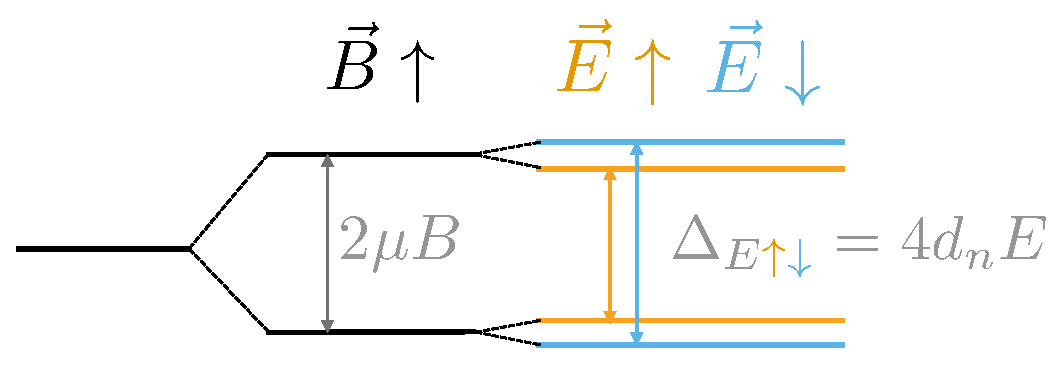
\includegraphics[width=0.7\linewidth]{gfx/introduction/measurement_principle.pdf}
  \caption{The energy states of a neutron in a combination of a magnetic and electric fields. The hamiltonian is $H = - 2 \left( \mu_\text{n} \, \bm{B} + d_\text{n} \, \bm{E} \right ) \cdot \bm{S}$. The first term causes the first splitting, $2\mu_\text{n} B$ large. The second term increases or decreases, for the electric field parallel and anti-parallel to the magnetic one respectively, the splitting by $2 d_\text{n} E$.}\label{fig:nEDM_measurement_principle}
\end{figure}

Already in 1949, before Wu's discovery of $P$-violation in the weak sector, Purcell and Ramsey performed a measurement to test $P$-violation in the strong sector using the nEDM as the probe~\cite{PhysRev.108.120}. They got a zero-consistent result $d_n = (-0.1 \pm 2.4) \times 10^{-20}\,\si{\elementarycharge\centi\meter}$.

Figure~\ref{fig:nEDM_measurement_principle} illustrates the energy of a neutron in a magnetic field $B$, where it has two energy states separated by $2 \mu_\text{n} B$. The apparatus of Purcell and Ramsey could measure this separation, as a frequency, very precisely. Additionally to the magnetic field, there was an electric one, either parallel or anti-parallel to it. If there had been an nEDM, the energy separation would have increased in one configuration and decreased in the other. The difference between the energy separations measured in the two field configurations is proportional to the nEDM $d_\text{n}$.

\begin{figure}
  \centering
  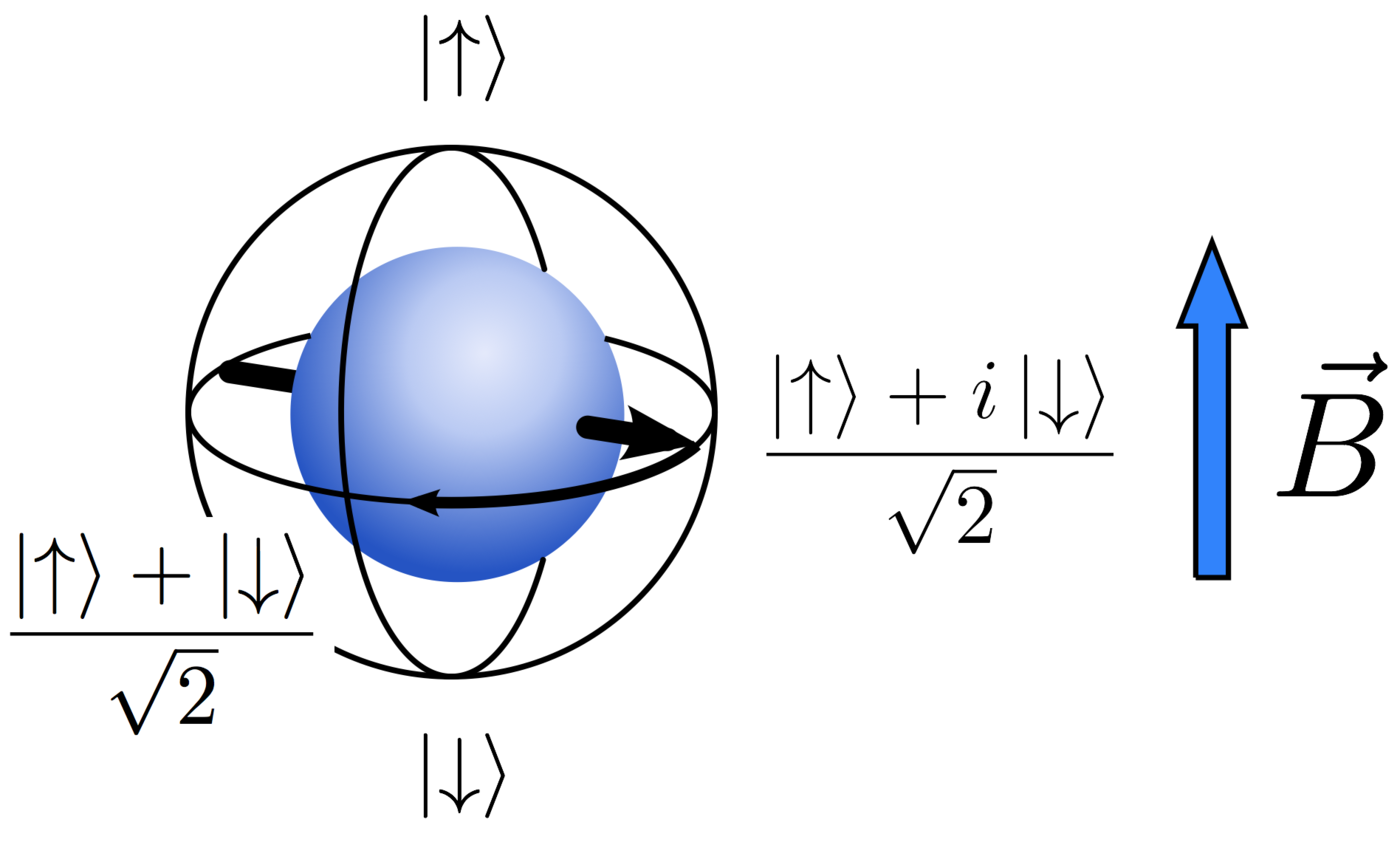
\includegraphics[width=.6\linewidth]{gfx/nEDMatPSI/bloch_sphere.png}
  \caption{A spin $\tfrac{1}{2}$ particle in a magnetic field on a Bloch sphere. The poles correspond to the pure spin-up and spin-down states. On the equator lie the states with an equal contribution of the two and the longitude corresponding to the quantum phase.}\label{fig:nEDM_bloch_sphere}
\end{figure}

To measure the energy separation between the two spin states they used what is now called the Ramsey method of separated oscillatory fields. In order to explain it, let us first consider a neutron in a magnetic field, as pictured in Fig.\,\ref{fig:nEDM_bloch_sphere}. The neutron's spin is depicted there on the Bloch sphere, where the poles correspond to the pure spin-up and spin-down states. On the equator lie the states with equal content of the two, the longitude marking the quantum phase. When the spin state is not vertical, the interaction between the magnetic moment and the magnetic field exerts a torque that sets it into rotational motion, called the Larmor precession. The frequency of the motion is proportional to the energy difference between the two states.
\note{Maybe don't mix classical and quantum pictures.}

\begin{SCfigure}
  \centering
  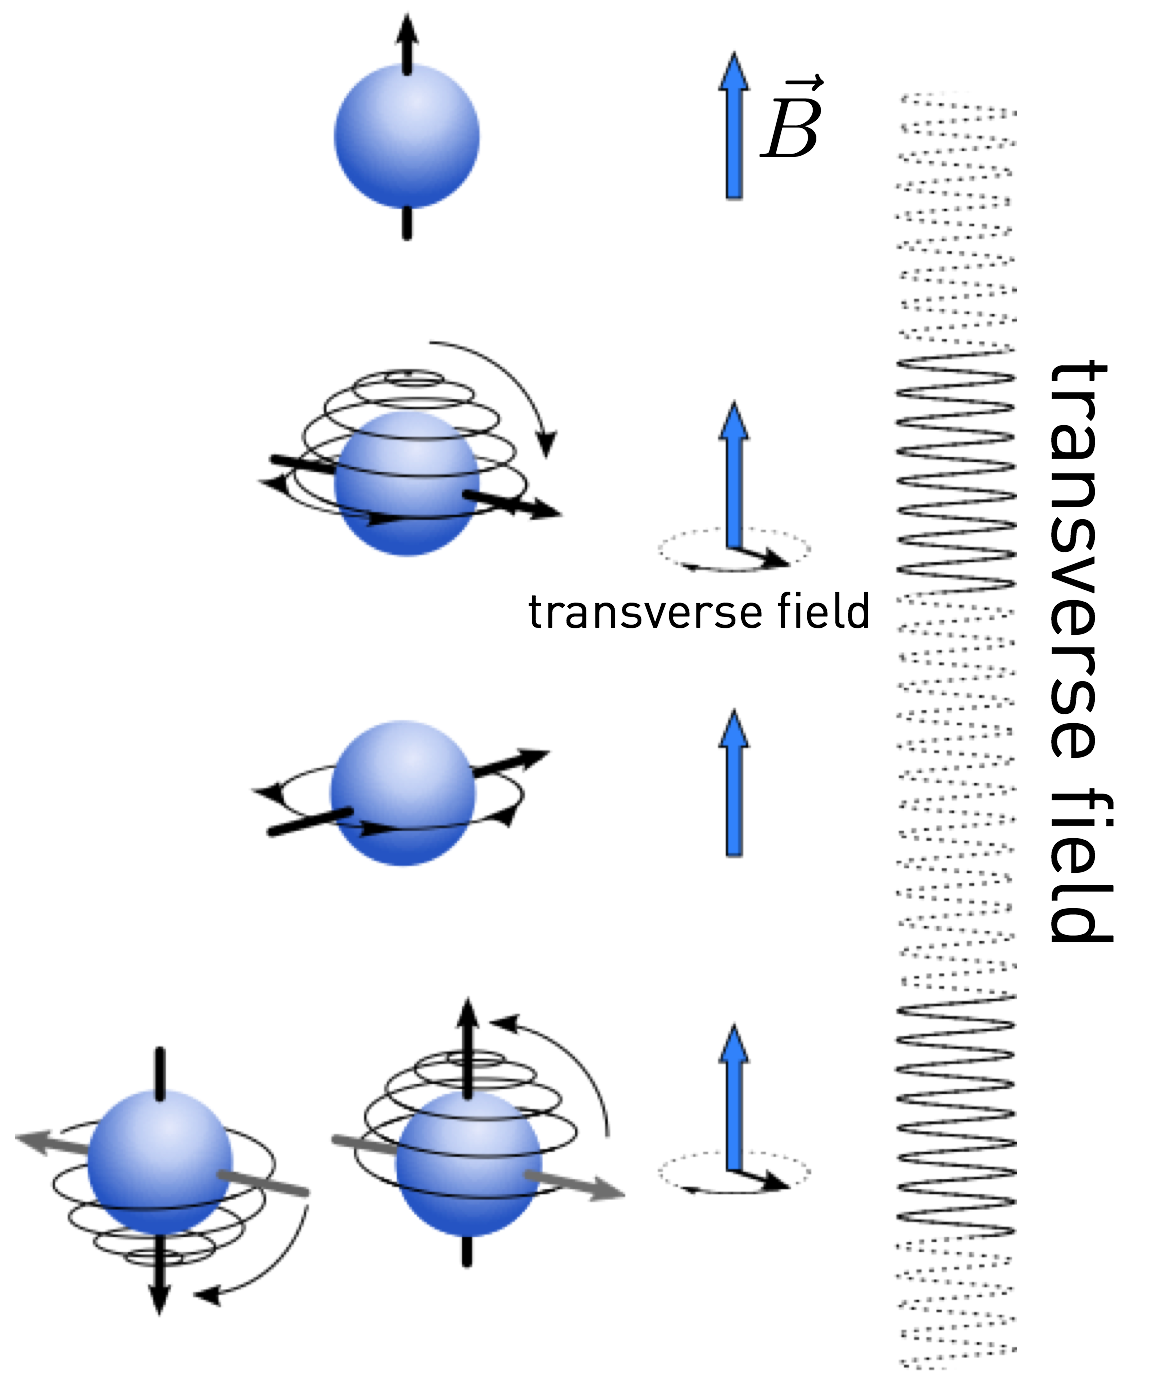
\includegraphics[width=.6\linewidth]{gfx/nEDMatPSI/Ramsey_principle.png}
  \caption{The principle of the Ramsey method, explained with the spin on the Bloch sphere. A polarised spin ensemble is in a magnetic field. A pulse of an oscillating transverse field flips the polarisation into the horizontal plane. The spin is allowed to freely precess in the field. Then, a second pulse of a transverse field is applied, in phase with the first one. The direction of the polarisation's flip depends on the relative phase between the spin and the transverse field.}\label{fig:nEDM_Ramsey_principle}
\end{SCfigure}

\begin{figure}
  \centering
  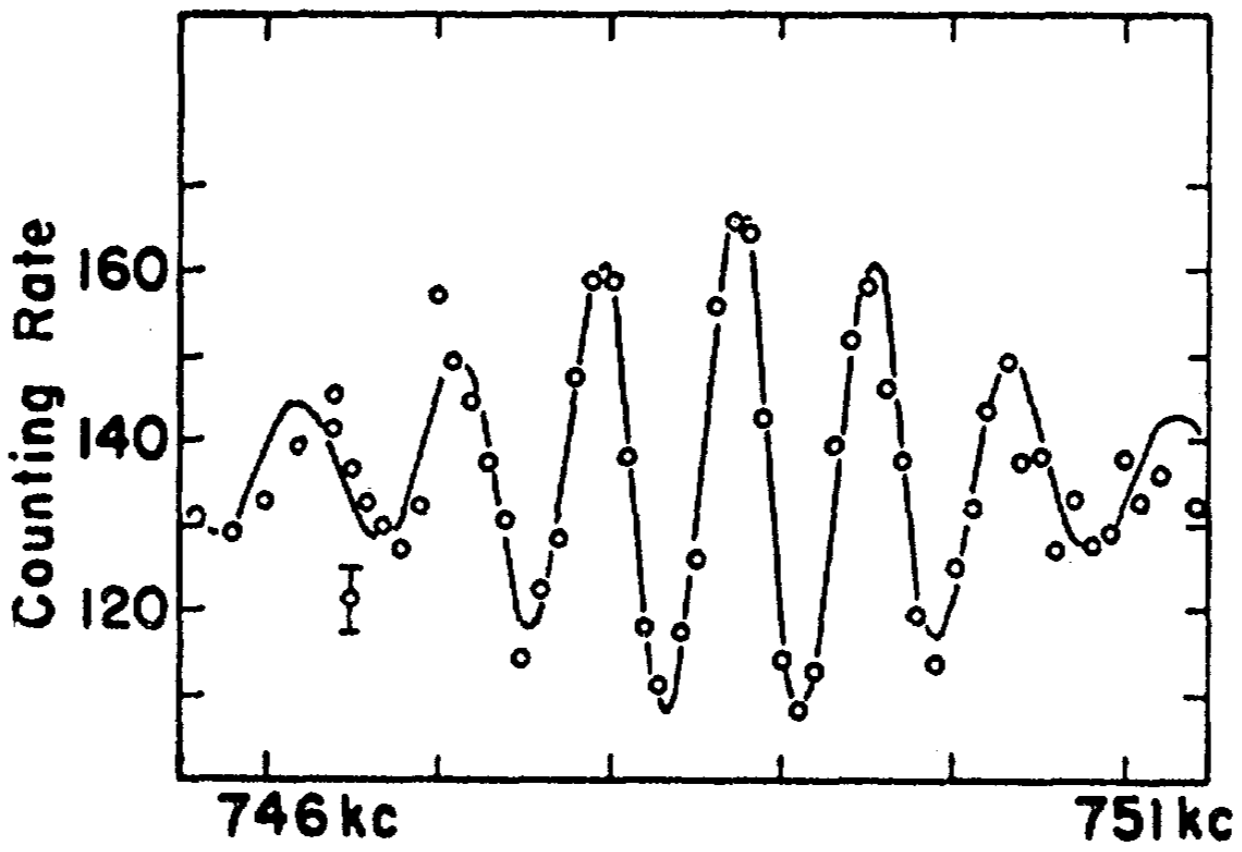
\includegraphics[width=.6\linewidth]{gfx/introduction/Ramsey_original_resonance.png}
  \caption{The original resonance curve measured by Ramsey~\cite{PhysRev.108.120}. The counting rate versus the frequency of the generator powering the spin-flipping coils. The fringes are due the interference between the precessing spins and the transverse field. Their width is the inverse duration of the free precession. The envelope arises, as at a large detuning the spins were not flipped into the horizontal plane anymore.}\label{fig:nEDM_Ramsey_original_curve}
\end{figure}

In the experiment a nearly monochromatic neutron beam passed through a polariser, a region with an electric field, an analyser, and hit a neutron counter at the end. The whole setup was in a magnetic field. At the beginning and the end of the region with the electric field, there were coils producing an oscillating magnetic field in the direction perpendicular to the main magnetic field. The spin evolution between the two coils is depicted in Fig.\,\ref{fig:nEDM_Ramsey_principle}. When a neutron precessing in a magnetic field feels an additional oscillating field, transverse to the main one and of frequency close to the Larmor one, its spin undergoes a nutation---the precession plane moves along the main field (North or South on the Bloch sphere). The direction is determined by the relative phase between the spin's precession and the transverse oscillating field. In Ramsey's experiment the length of the coils was set to flip the neutrons' spins by $\pi/2$, so that after having passed the first coil they were precessing on the Bloch sphere's equator. The direction of the nutation in the second coil, and with it the probability of passing the analyser, depended on the relative phase between the precession and the transverse field. A slight change in the frequency of the generator powering the coils caused a considerable change in the phase difference that builded up while the neutrons flew precessing between the coils. Scanning the frequency of the generator and monitoring the counting rate produced a resonance curve (Fig.\,\ref{fig:nEDM_Ramsey_original_curve}). The middle of the central fringe is the resonance frequency corresponding to the transition energy between spin-up and spin-down states. Comparing the positions of the resonance with the magnetic and electric fields parallel and anti-parallel gave the $d_n$ estimate.

\begin{figure}
  \centering
  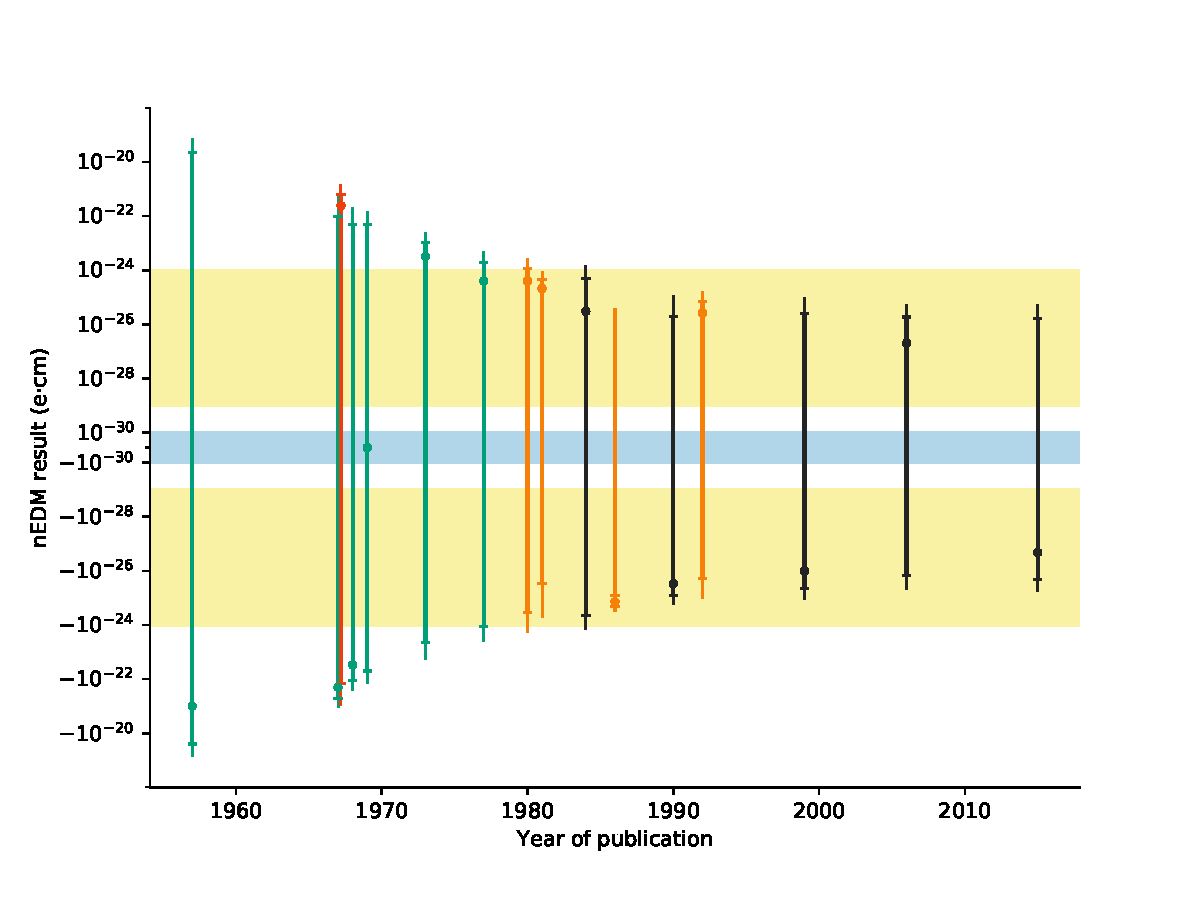
\includegraphics[width=\linewidth]{gfx/introduction/edm_limits.pdf}
  \caption{The history of the neutron electric dipole moment measurements. For each published result the vertical line corresponds to the $3\upsigma$ allowed region, horizontal bars depict the $1\upsigma$ one. The data markers are located at the central values of the measurements. The vertical scale is a combination of two logarithmic ones---one for each sign of nEDM\@. The region of the Standard Model's prediction is depicted in blue, the one of the proposed Model's extensions in yellow. The red line indicates a result obtained from a neutron scattering experiment. The sources are, in chronological order:~\cite{PhysRev.108.120,PhysRevLett.19.381,PhysRevLett.19.384,PhysRev.170.1200,PhysRev.179.1285,PhysRevD.7.3147,PhysRevD.15.9,ALTAREV1980269,ALTAREV198113,altarev1986search,ALTAREV1992242,PENDLEBURY1984327,SMITH1990191,PhysRevLett.82.904,PhysRevLett.97.131801,Pendlebury2015}}\label{fig:nEDM_limits_history}
\end{figure}

\marginpar{In the LNPI measurements slightly differ from Ramsey's technique. Instead of spin-flips, they used an adiabatic transition in inhomogeneous magnetic field, in order to account for different storage times of individual neutrons freely travelling through the bottle.}
The community uses this technique to measure the nEDM until this day, their ever-more-sensitive efforts summarised in Fig.\,\ref{fig:nEDM_limits_history}. Until 1970s the measurements were done using a beam of cold neutrons (marked in green), after then storage experiments greatly improved the time of the free precession and thereby the sensitivity. It was made possible by neutrons with kinetic energies below approximately \SI{300}{\nano\electronvolt} (referred to as ultracold), which storable in some materials, by undergoing a total internal reflection~\cite{UCNbook}. In 1980 in the Leningrad Nuclear Physics Institute (LNPI, former USSR) the first measurement was performed with the neurons being stored in a bottle~\cite{ALTAREV1980269}. The measurements in LNPI continued (orange) and in 1984 were joined by an international effort in the Institute Laue--Langevin in France (black).

In 2007 a new effort has begun in the Paul Scherrer Institute (PSI) in Villigen, Switzerland. The experiment collected data over the years 2015--17 and at the time of writing the result was still being evaluated. The author had the honor to be part of this venture, which we will take a closer look at in the next chapter. The description of the nEDM measurement at PSI serves as an introduction to the main part of this work, the original work of the author, which focuses on two aspects closely related to all nEDM measurements: stabilisation of magnetic fields and exotic physics that can be explored with those highly sensitive experiments.



\section{Magnetic stability}
The quality of the magnetic field is the main challenge in the measurements of the nEDM\@. Recall the principle of the measurement, as depicted in Fig.\,\ref{fig:nEDM_measurement_principle}. The electric dipole moment $d_\text{n}$ is proportional to the difference in the measured energy separations between the field configurations. Let us ask ourselves the following question: How big is a change in the magnetic field that causes a comparable change in the separation of the states?

The current nEDM limit is around $|d_\text{n}| < \SI{e-26}{\elementarycharge\centi\meter}$~\cite{PhysRevLett.97.131801}. Taking the electric field to be $\frac{ \SI{132}{\kilo\volt} }{ \SI{12}{\centi\meter} }$, as in the PSI experiment, this corresponds to an energy difference
\begin{equation}
  \Delta_{E\uparrow\downarrow} = 4 d_\text{n} E = \SI{4e-26}{\elementarycharge\centi\meter} \ \frac{ \SI{132}{\kilo\volt} }{ \SI{12}{\centi\meter} } = \SI{4.4e-22}{\electronvolt} \ .
\end{equation}
With the approximate neutron magnetic dipole moment~\cite{PDG2016}
\begin{equation}
  \mu_\text{n} = \SI{-9.7e-27}{\joule\per\tesla} = \SI{-6e-8}{\electronvolt\per\tesla} \ ,
\end{equation}
the size of a change in magnetic field corresponding to this energy is
\begin{equation}
  \frac{ \Delta_{E\uparrow\downarrow} }{2 \mu_n} = \SI{3.7e-15}{\tesla} = \SI{3.7}{\femto\tesla} \ .
\end{equation}
\marginpar{In reality the requirement is relaxed by a factor of 10--100, as the final measurement is an average of several thousand measurements.}
This is about the strength of the magnetic field of a car passing several kilometers away. The field needs to be controlled on this level so that the two measurement, with the magnetic and electric fields parallel and anti-parallel, can be subtracted from one another without the difference not being dominated by the instability of the magnetic field.
% Even in the most quiet of nights the magnetic field at the experimental site was not more stable than about a nanotesla, and during a day the variations reached tens of microteslas.

The nEDM experiments continue to set the world's standard in terms of stabilising and measuring magnetic fields~\cite{GREEN1998381,1748-0221-10-12-P12003,Groeger2005,Baker2014}. When it comes to stabilisation, a newcomer in the field is an active magnetic field stabilisation system. It was first used in the nEDM measurement at PSI, increasing the field stability by a factor of 5--50~\cite{Afach2014}. The second part of this work is dedicated to research in this area. A novel method of designing coils is introduced, which makes active stabilisation systems more compact and effective. It is followed by a presentation of a system constructed at the ETH Zürich, intended as a small-scale prototype of a next-generation system for the nEDM measurement at PSI\@. Finally, a survey of the magnetic field at PSI's experimental area is described, a part of research on the magnetic field compensation there.



\section{New physics}
nEDM experiments can be sensitive to, next to the electric dipole moment, other new physics. For example, a search for a short range spin-dependent interaction mediated an axion, a hypothetical new particle~\cite{Afach2015Exotic}; or testing the Lorentz invariance by looking for variations arising due to the Earth spinning in an non-isotropic Universe~\cite{Altarev2009,ALTAREV20112365}; or searching for mirror particles, proposed to restore the global $P$-symmetry, by detecting neutron to mirror-neutron oscillations with an nEDM apparatus~\cite{PhysRevD.80.032003}.

The author is proud to have taken part in starting a new area of dark matter searches with nEDM experiments. One of the candidates for dark matter are axions, extremely light particles generalising the idea of promoting the $\theta_\text{QCD}$ parameter (the same as in the strong $CP$ problem) into a field~\cite{PhysRevLett.38.1440}. An axion dark matter would form a coherently, very slowly (as slowly as days) oscillating field. This would induce coherent variations in the measured values of nEDM\@. A search for such variations is discussed in the part three.
\chapter{nEDM measurement in PSI}
\label{ch:nedm-at-psi-apparatus}

% \section{The collaboration}
The nEDM-at-the-PSI collaboration has been founded to perform an nEDM measurement in the Paul Scherrer Institute (PSI) in Villigen, Switzerland. The experiment had been planned in two stages. In the first stage, the apparatus used in the ILL experiment was moved to PSI, where it was installed to benefit from a new, highly intense source of ultracold neutrons~\cite{Lauss2014}. The first stage finished in Autumn 2017, after having collected enough statistics to set the world's best limit (Fig.\,\ref{fig:nEDM_accumulated_sensitivity}). As of Spring 2018 the analysis is still ongoing.

\begin{figure}
  \centering
  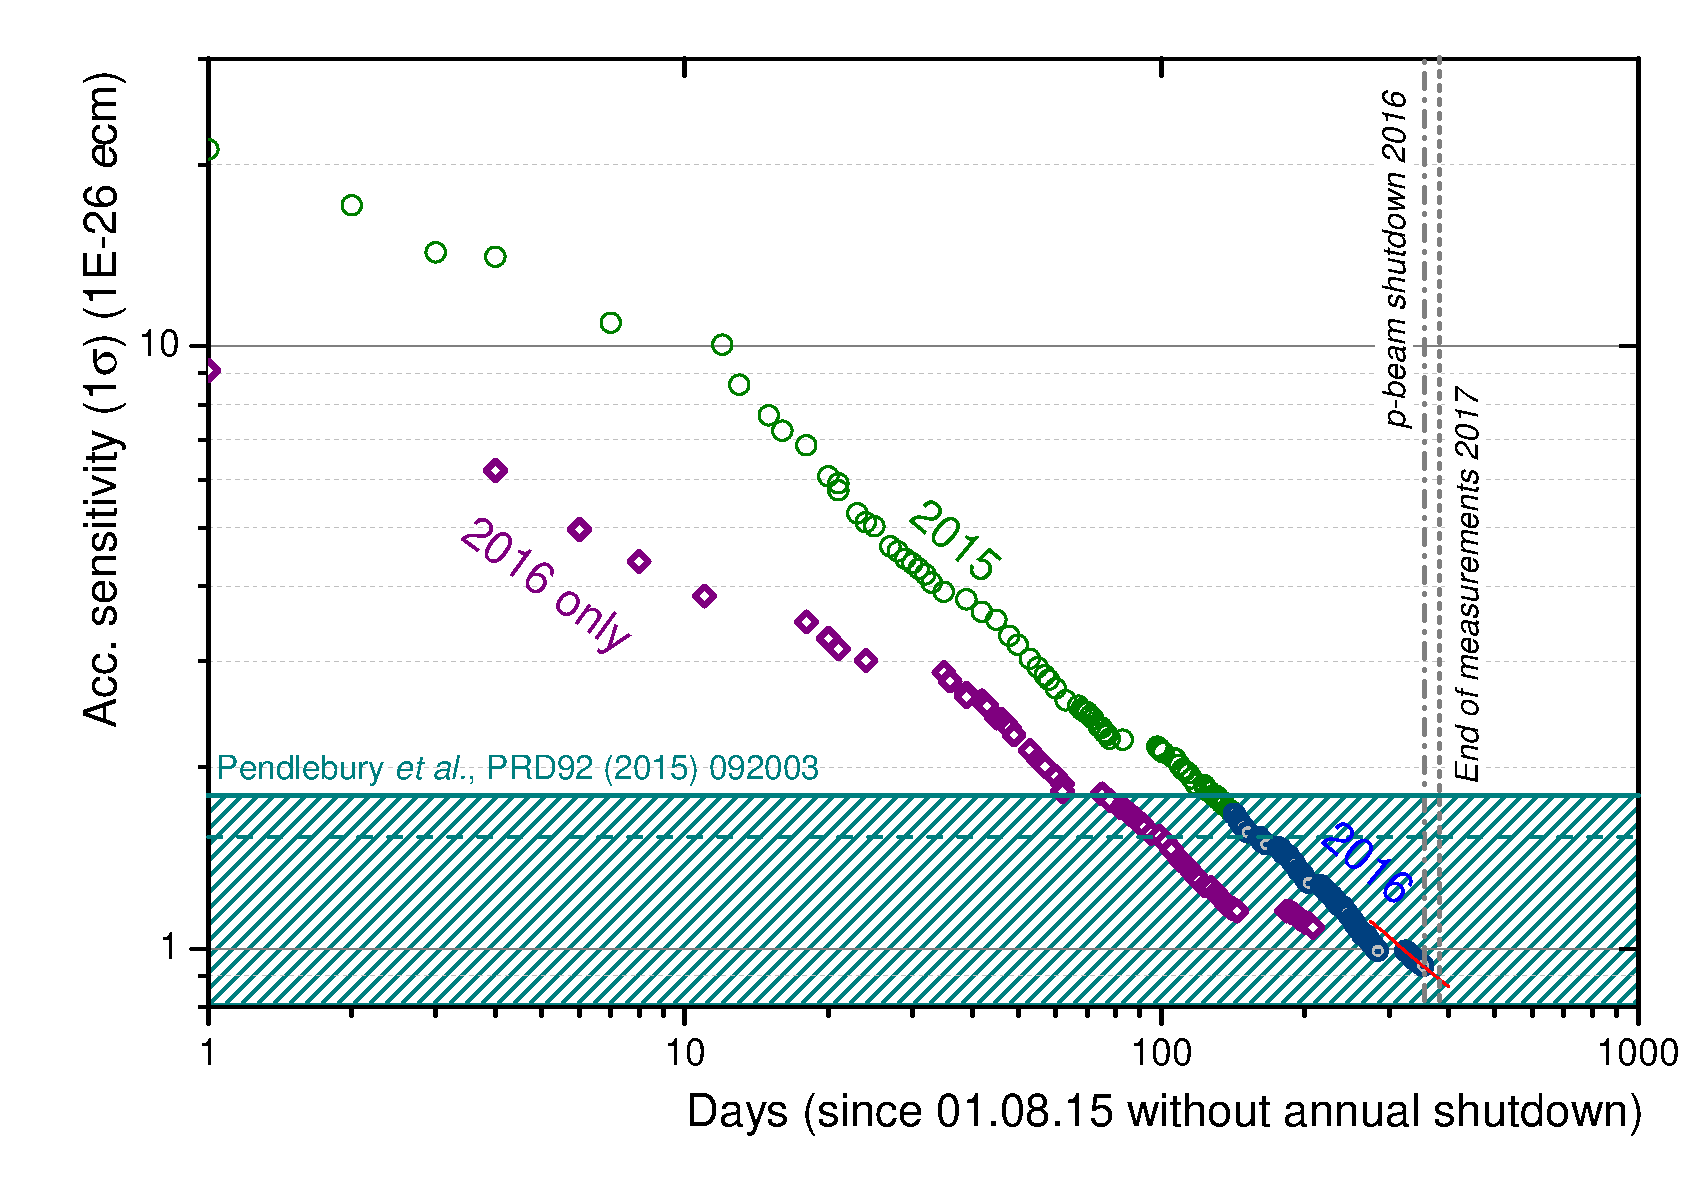
\includegraphics[width=0.8\linewidth]{gfx/nEDMatPSI/accumulated_sensitivity.pdf}
  \caption{The accumulated statistical sensitivity of the nEDM-at-PSI experiment. The sensitivity of the data collected in 2015 is shown in green, of 2015 and 2016 in blue, and only 2016 in violet. The dashed region marks the yet unexplored area below the best limit~\cite{Pendlebury2015}. Courtesy of Dr. Philipp Schmidt-Wellenburg.}
  \label{fig:nEDM_accumulated_sensitivity}
\end{figure}

Already in the first stage the apparatus underwent numerous improvements, leaving only few parts of the original. The improvements were part of the research and development plan for the second stage, a newly built apparatus called n2EDM. The new experiment, designed by the personnel experienced with running, modifying and improving the first stage, would have the goal of exploring the \SI{e-27}{\elementarycharge\centi\meter} range.


\section{The apparatus}
This work focuses on the stage-one apparatus. It employed the Ramsey method with ultracold neutrons stored for the time of the precession. The neutrons, produced in the source, were guided with a pipe system into a storage chamber, where they underwent the Ramsey procedure. The polarisation was then measured by letting the neutrons fall into a spin-state--sensitive neutron detector. A diagram of the system is shown in Fig.\,\ref{fig:nEDM_scheme}.

\begin{figure}
  \centering
  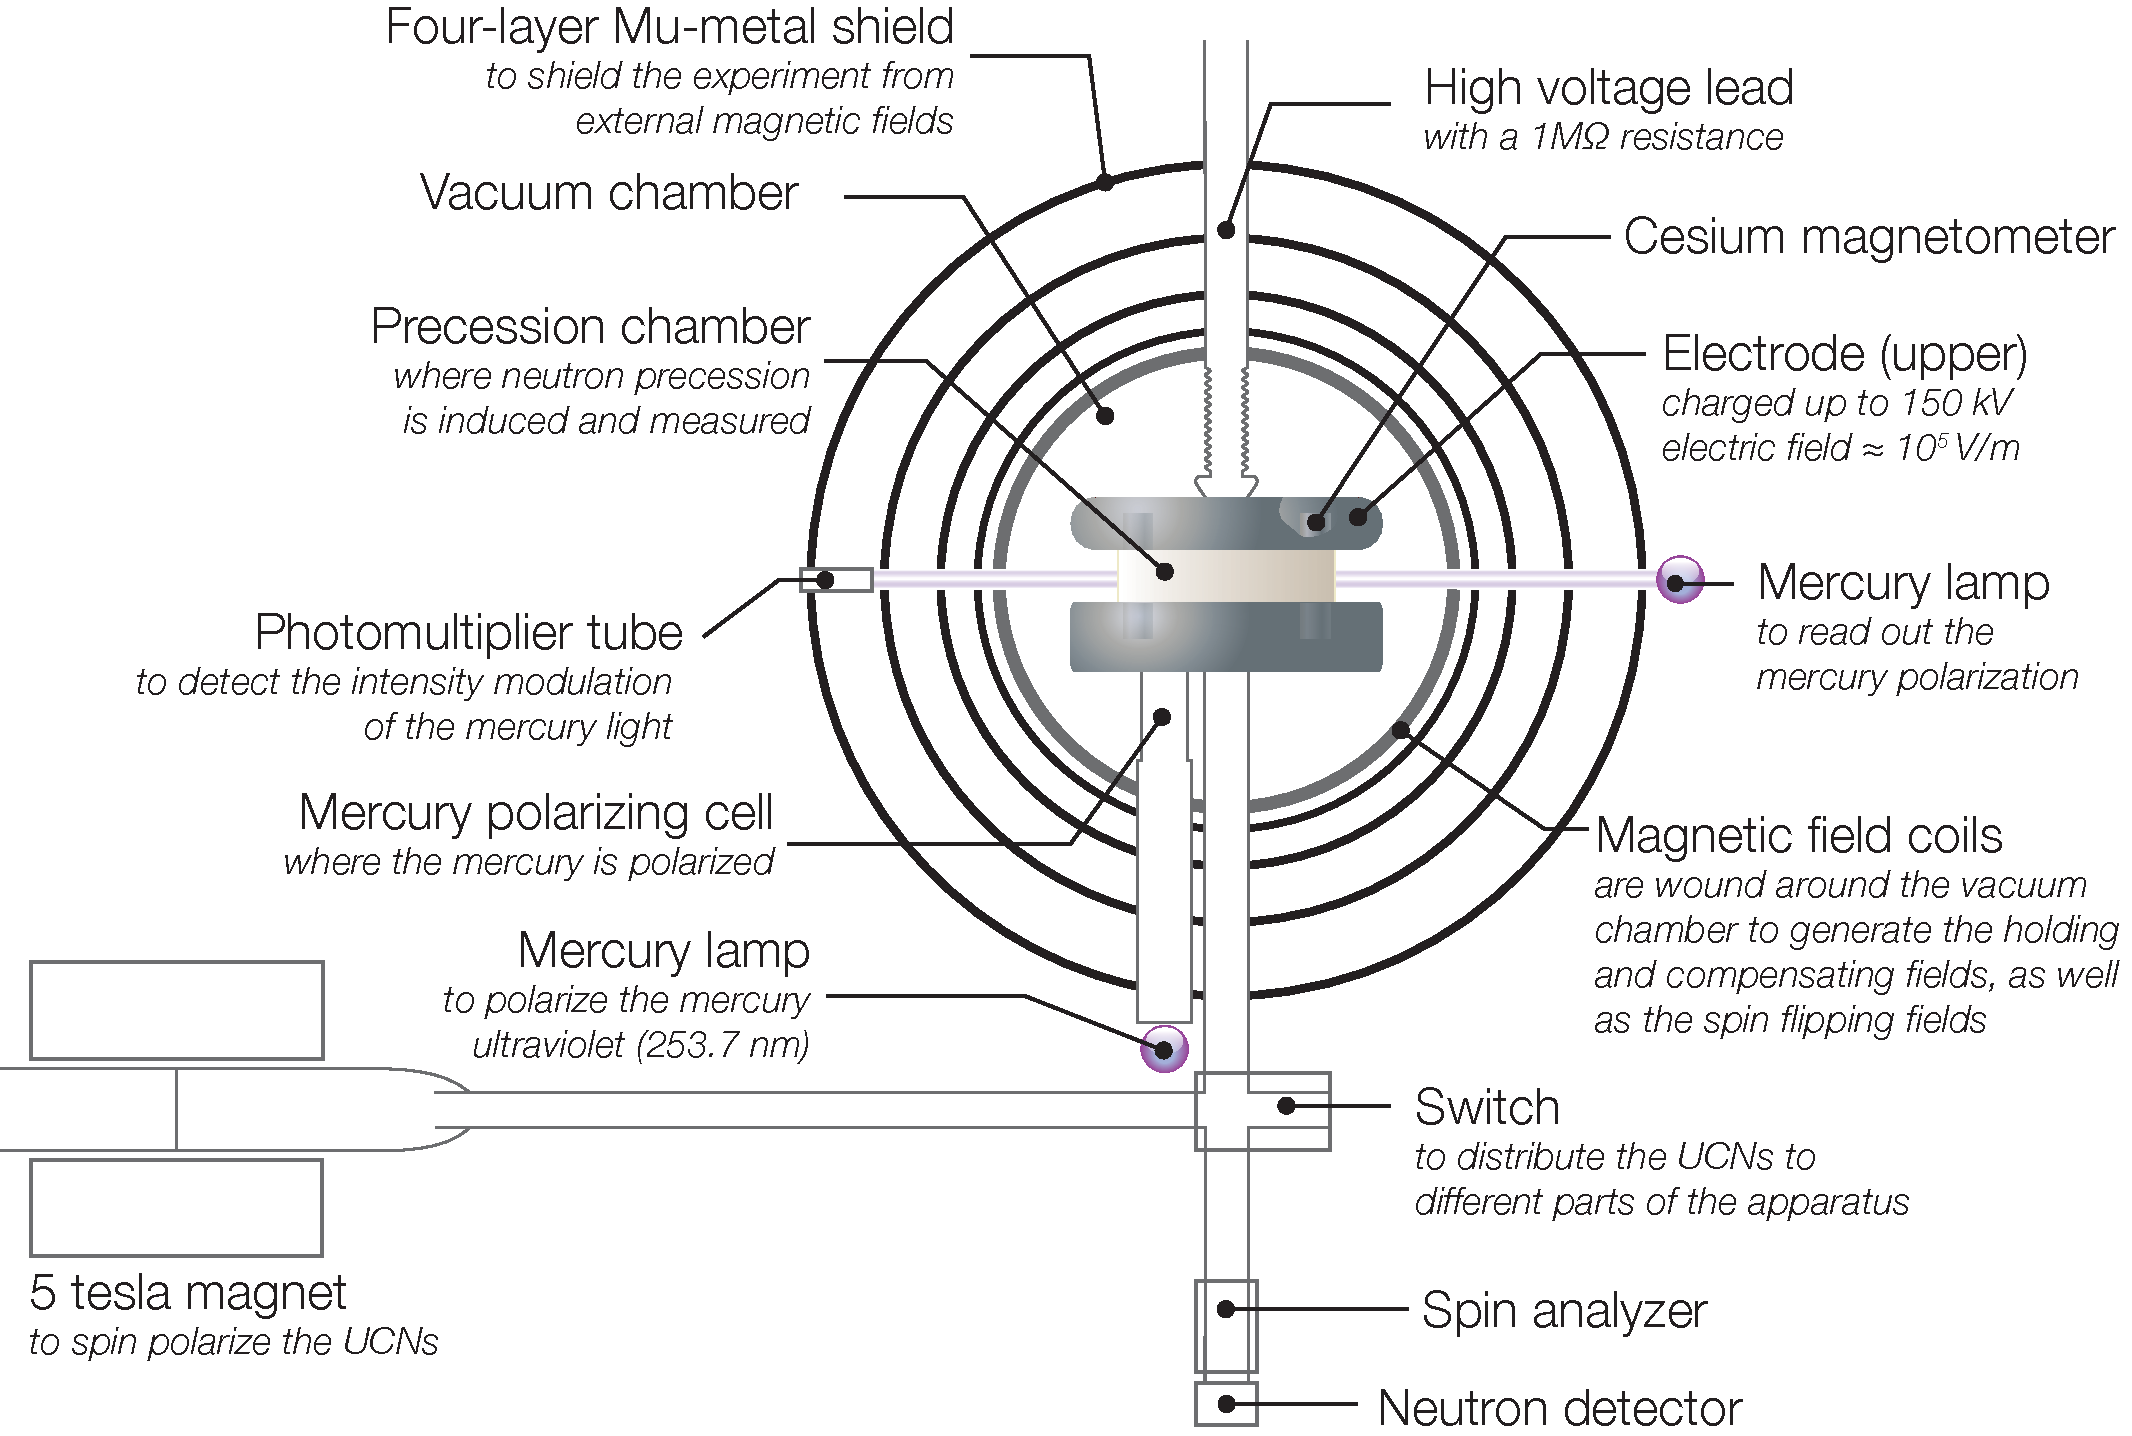
\includegraphics[width=\linewidth]{gfx/nEDMatPSI/apparatus-cartoon-main-and-sub-labels.pdf}
  \caption{The scheme of the nEDM-at-PSI apparatus. \note{Whom to credit for the image? Make my own? No\ldots}}
  \label{fig:nEDM_scheme}
\end{figure}

A single measurement cycle was triggered by a pulse of ultracold neutrons incoming from the PSI source. The neutrons were guided in metal-coated glass pipes. First, they were polarised by passing through a five-tesla magnet. Then, a rotary three-way valve, called the switch, directed the neutrons upwards into a vacuum tank, where they filled a \SI{12}{\centi\meter}-high cylindrical precession chamber. The chamber was sandwiched between high-voltage electrodes, charged to \SI{132}{\kilo\volt}, which created an electric field in the chamber. The whole stack was submerged in a \SI{1}{\micro\tesla} vertical magnetic field $B_0$. Once the neutrons filled the cylinder, the entrance was shut close and the particles were stored for around \SI{200}{\second} to undergo the Ramsey procedure.

First, a pulse of oscillating transverse field was applied, with its amplitude and length tuned, so that the the neutrons' spins flip from the vertical orientation, along the $B_0$ field, to the horizontal plane. This set the spins into a Larmor precession.
\marginpar{The nEDM-at-PSI experiment the neutrons were dropped into two-armed detector, capable of counting both spin states simultaneously~\cite{Afach2015USSA}.}
After \SI{180}{\second} a second pulse, in phase with the first one, was applied. Then the chamber's entrance was opened, and the neutrons were allowed to fall through the switch and a spin analyser into the neutron detector.


The purpose of rest of the components, in fact---the majority, is either providing a stable magnetic field environment in the precession chamber or measuring the field.




\section{Magnetic fields}
\marginpar{The exact attenuation factor of the shield depended on the direction and varied from 1600 to 13300~\cite{Komposch2017}.}
The most important measure of stabilising the magnetic field is passive shielding. The vacuum tank, with the precession chamber in it, was covered by four layers of highly permeable material, called $\upmu$-metal.
Each layer attenuated the magnetic field changes by a factor of approximately ten. The high magnetic permeability of the $\upmu$-metal makes the magnetic field much rather go inside the metal and around the volume it encloses, than to penetrate into the volume. 
%Even though $\upmu$-metal provided excellent shielding properties, as a ferromagnetic it distorts the field both outside and inside the shield. Also it had to be regularly demagnetised.

Inside the shield, on the vacuum chamber, there were a number of coils wound. The main magnetic field $B_0$ was produced by a cos-theta coil.
\marginpar{In an ensemble precessing in an inhomogenous field, members in different places precess at slightly different rates. This leads to depolarisation by the loss of coherence.}
Besides, there were numerous others, producing field of various shapes.
They were, on one hand, used to homogenise the field, which reduced the depolarisation rate of the neutrons,
and on the other, to deliberately apply vertical gradients $\partial_z B_0$ (operating in different gradients was part of the measurement procedure and is explained later in this chapter).

The stability of the field inside the shield was in the picotesla range. The remaining variations were measured and corrected for, primarily with a mercury-based magnetometer~\cite{FertlThesis,Komposch2017}. Below the precession chamber there was a cell containing a vapour of polarised $^{199}$Hg atoms, which was released into the precession chamber once it had been filled with neutrons.
\marginpar{In the \SI{1}{\micro\tesla} $B_0$ field the precession frequencies of neutrons and $^{199}$Hg atoms are approximately \SI{30}{\hertz} and \SI{8}{\hertz}, respectively. The respective spin-flip pulses affect the other spices only very slightly.}
There, a dedicated spin-flip pulse of an oscillating transverse magnetic field started their coherent precession, which was read on-line optically. A mercury discharge lamp shone a circularly polarised light through the precession chamber onto a photomultiplier tube. As the mercury atoms' photon-capture cross-section depended on the phase of the precession, the transparency of the chamber to the polarised light oscillated at the mercury's Larmor frequency. The oscillating signal of the photomultiplier was then analysed to estimate its frequency, proportional to the $B_0$ field, as averaged by the mercury atoms.

The mercury magnetometer may seem an ideal measure to correct the neutron measurement for the drifts of the magnetic field, as the two spices filled exactly the same volume (hence it is often called a \emph{comagnetometer}). Only, not exactly. The ultracold neutrons were slow enough to be affected by the gravity, which shifted their centre of mass around \SI{2.4}{\milli\meter} relative to the warm, homogeneous mercury vapour~\cite{Afach2014magmoment}. In a presence of a vertical gradient, the two spices saw different fields. A detailed discussion of additional systematic effects related to this magnetometer can be found in~\cite{Afach2014magmoment}.

A way to measure vertical gradients, as well as other high-order components of the magnetic field, was provided by an array of Caesium magnetometers~\cite{Groeger2005}. These sensors were located inside the electrodes---seven in the top one, nine in the bottom one. Each magnetometer was a cell filled with Caesium vapour, through which a circuraly polarised light, delivered with a light guide, shone at \SI{45}{\degree} inclination angle. The light simultaneously polarised the atoms and, as it met a surface of a photodiode behind the cell, probed their precession. A coil wound around the cell, axial with the light beam, was driven in a feedback loop with the diode's signal to resonantly drive the Larmor precession. Even though the magnetometers measured only the magnitude of the magnetic field, they provided information about the higher-order components of the field thanks to their distribution around the chamber. For example, one could na\"\i vely estimate the vertical gradient $\partial_z B_z$ by evaluating the average readings of the sensors in each electrode, taking the difference and dividing by the vertical separation. Actually, the high-order field terms, including the vertical gradient, were obtained by fitting a second-order parametrization of the magnetic field to the readings of the sensors~\cite{WurstenThesis}.

In the next section we describe how all these components came together to perform a measurement of the electric dipole moment of the neutron.



\section{Measurement procedure}
\label{sec:measurement_procedure}

\begin{figure}
  \centering
  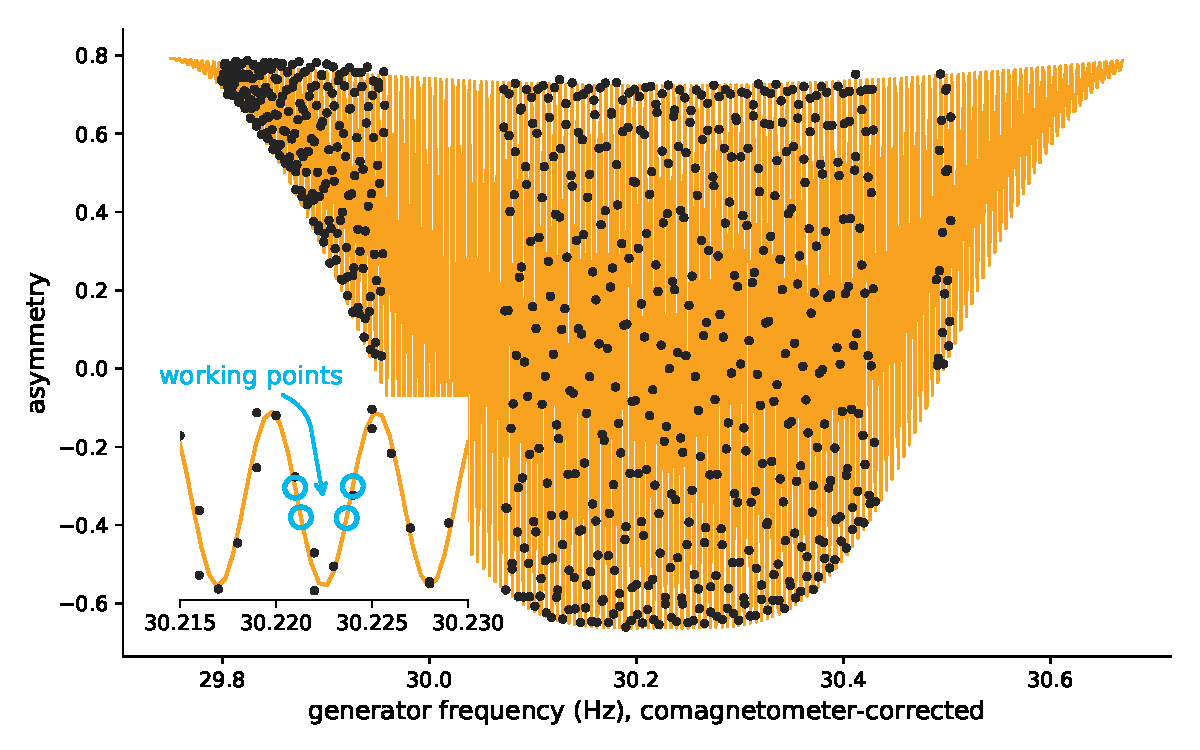
\includegraphics[width=0.8\linewidth]{gfx/nEDMatPSI/ramsey_scan.pdf}
  \caption{A scan of the Ramsey resonance curve in the nEDM experiment at the PSI---the asymmetry is measured as the function of the detuning of the spin-flip generator's frequency. The black points depict the measured points, the orange line is the fit of the theoretical model. In the inset, the central fringe is enlarged and the working points are marked, which is where the experiment took data during normal operation. The generator frequency has been corrected with the $^{199}$Hg comagnetometer using the formula $\nu_\text{generator} / \nu_\text{Hg} \times \overline{\nu_\text{Hg}}$, where $\overline{\nu_\text{Hg}}$ is the average over the scan.}
  \label{fig:ramsey_scan}
\end{figure}

Recall the Ramsey method (Fig.\,\ref{fig:nEDM_Ramsey_principle}). Two coherent pulses of a transverse oscillating field are applied to an ensemble of polarised neutrons, with a period of free precession in between. Measuring the polarisation after the second pulse as the function of the frequency of the transverse field yields a resonance curve. The curve measured in the PSI experiment is reproduced in Fig.\,\ref{fig:ramsey_scan}. Comparing it with Ramsey's original curve (Fig.\,\ref{fig:nEDM_Ramsey_original_curve}) summarises fifty years of progress in measuring the electric dipole moment of the neutron.

In the normal operation not the whole curve was sampled, but only the region most sensitive to the position of the central fringe---its steepest slope. In Fig.\,\ref{fig:ramsey_scan} the four \emph{working points} are marked, which the experiment was programmed to aim at. Assuming all the data are taken in this most sensitive region, the sensitivity for the nEDM is~\cite{FertlThesis}:
\begin{equation}
  \sigma(d_\text{n}) = \frac{\hbar}{ 2 \alpha E T \sqrt{N} } \ ,
\end{equation}
where $\alpha$ is the relative height of the curve ($\alpha = 1$ means the curve spanning from $-1$ to $1$ in asymmetry), $E$ is the strength of the electric field, $T$ is the duration of the free precession (\SI{180}{\second}, its inverse is the width of the fringes), and $N$ is the counting statistics. It is the statistical limit on the sensitivity, the value obtained from the analysis is expected be slightly worse.

Each cycle of the experiment, filling in the neutrons, performing the Ramsey procedure and counting them, sampled one of the working points on the resonance curve. Assuming that the only parameter that changed between the cycles was the position of the resonance (due to drifts of the field), one could estimate the position of the central fringe, the neutron precession frequency $\nu_\text{n}$ for each cycle. In other words, the neutrons were a very accurate magnetometer operating on a cycle basis.
% The resonance frequency $f_n^{\,0}$ is determined with a fit of the resonance curve. Because the points are probed one after another, it is only possible after a set of data points, \emph{cycles}, have been measured. In order to extract the neutron precession frequency for each individual \emph{cycle}, one assumes that the only parameter of the resonance curve that varies on a cycle--to--cycle basis is the position of the resonance. With this assumption the shape of the curve, fitted to the whole set of \emph{cycles}, is used to calculate back the resonant frequency in each \emph{cycle} of the set.

Naturally, measuring the magnetic field with the neutrons was not the goal. It was the much, much smaller, if any, effect of the electric field on the precession frequency that the experiment was after. To even out the variations in $\nu_\text{n}$, its ratio to the frequency of the comagnetometer's mercury atoms $\nu_\text{Hg}$ was used instead:
\marginpar{This correction was already included in the depiction of the resonance curve in Fig.\,\ref{fig:ramsey_scan}.}
\begin{equation}
  \label{eq:Rdefinition}
  R \equiv \frac{\nu_\text{n}}{\nu_\text{Hg}} = \frac{\mu_\text{n}}{\mu_\text{Hg}} \pm \left( d_\text{n} \mp \frac{\mu_\text{n}}{\mu_\text{Hg}} \, d_\text{Hg} \right) \frac{2 E}{ h  \nu_\text{Hg}} + \Delta \ ,
\end{equation}
where the signs correspond to the parallel and anti-parallel configuration of the magnetic and electric fields. (The derivation of the formula can be found in App.\,\ref{ch:R_derivation_appendix}.)
It is immediately visible that $R$ is sensitive to $d_\text{n}$ just as $\nu_\text{n}$, but the fluctuations due the changes of the magnetic field are suppressed.
\marginpar{$R$ is actually sensitive to $d_\text{n} - \frac{\mu_\text{n}}{\mu_\text{Hg}} \, d_\text{Hg}$, but it has been measured that $|d_\text{Hg}| < \SI{7.4e-30}{\elementarycharge\centi\meter}$~\cite{PhysRevLett.116.161601}.}
$\Delta$ encapsulates all higher-order terms and systematic effects. In particular, the already mentioned effect due to the gravitational sag of the neutrons' population, relative to the geometrical centre of the chamber, in combination with a vertical gradient of the magnetic field.
% Together with the UCNs there is a polarised $^{199}$Hg gas precessing. Its precession is monitored with light, allowing for direct determination of the $^{199}$Hg Larmor frequecy and thus the magnetic field strength. In order to cancel the first-order magnetic field changes one looks at the value:
% \begin{equation}
%   R := f_n / f_{Hg} \ .
% \end{equation}
% However, the UCNs are cold enough to have their centre of mass shifted downwards a few centimeters by the gravity. The $^{199}$Hg gas, being much hotter then the UCNs, fills the precession volume homogeneously. In a presence of a vertical magnetic field gradient this causes the two species to see different magnetic fields.

% The largest effect in $\Delta$ has to do with the gradient of the magnetic field. The neutrons and mercury did not sample exactly the same field. The mercury vapour was at room temperature and filled the precession volume homogeneously. At the same time, the ultracold neutrons had an energy of only around \SI{300}{\nano\electronvolt}, while their gravitational potential is $m_\text{n} = \SI{102}{\nano\electronvolt\per\meter}$ steep~\cite{Zenner2013}. In effect, they filled, and sampled, the bottom of the chamber more then the top. The difference between centres of masses of the mercury and the neutrons was around \SI{4}{\mili\meter}


To get the $d_n$ estimate the electric field needed to be modulated. The experiment automatically reversed the polarisation of the electric field every 72 cycles. In between the two polarisations a few cycles were measured without the electric field (a total of 10\% of the data, which are not sensitive to the nEDM). Then a linear model of  $R$ vs. $E$ yielded an estimate of the electric dipole moment, which we call $d_n^*$ (Eq.\,\ref{eq:Rdefinition}, Fig.\,\ref{fig:crossing_lines}).

\begin{figure}
  \centering
  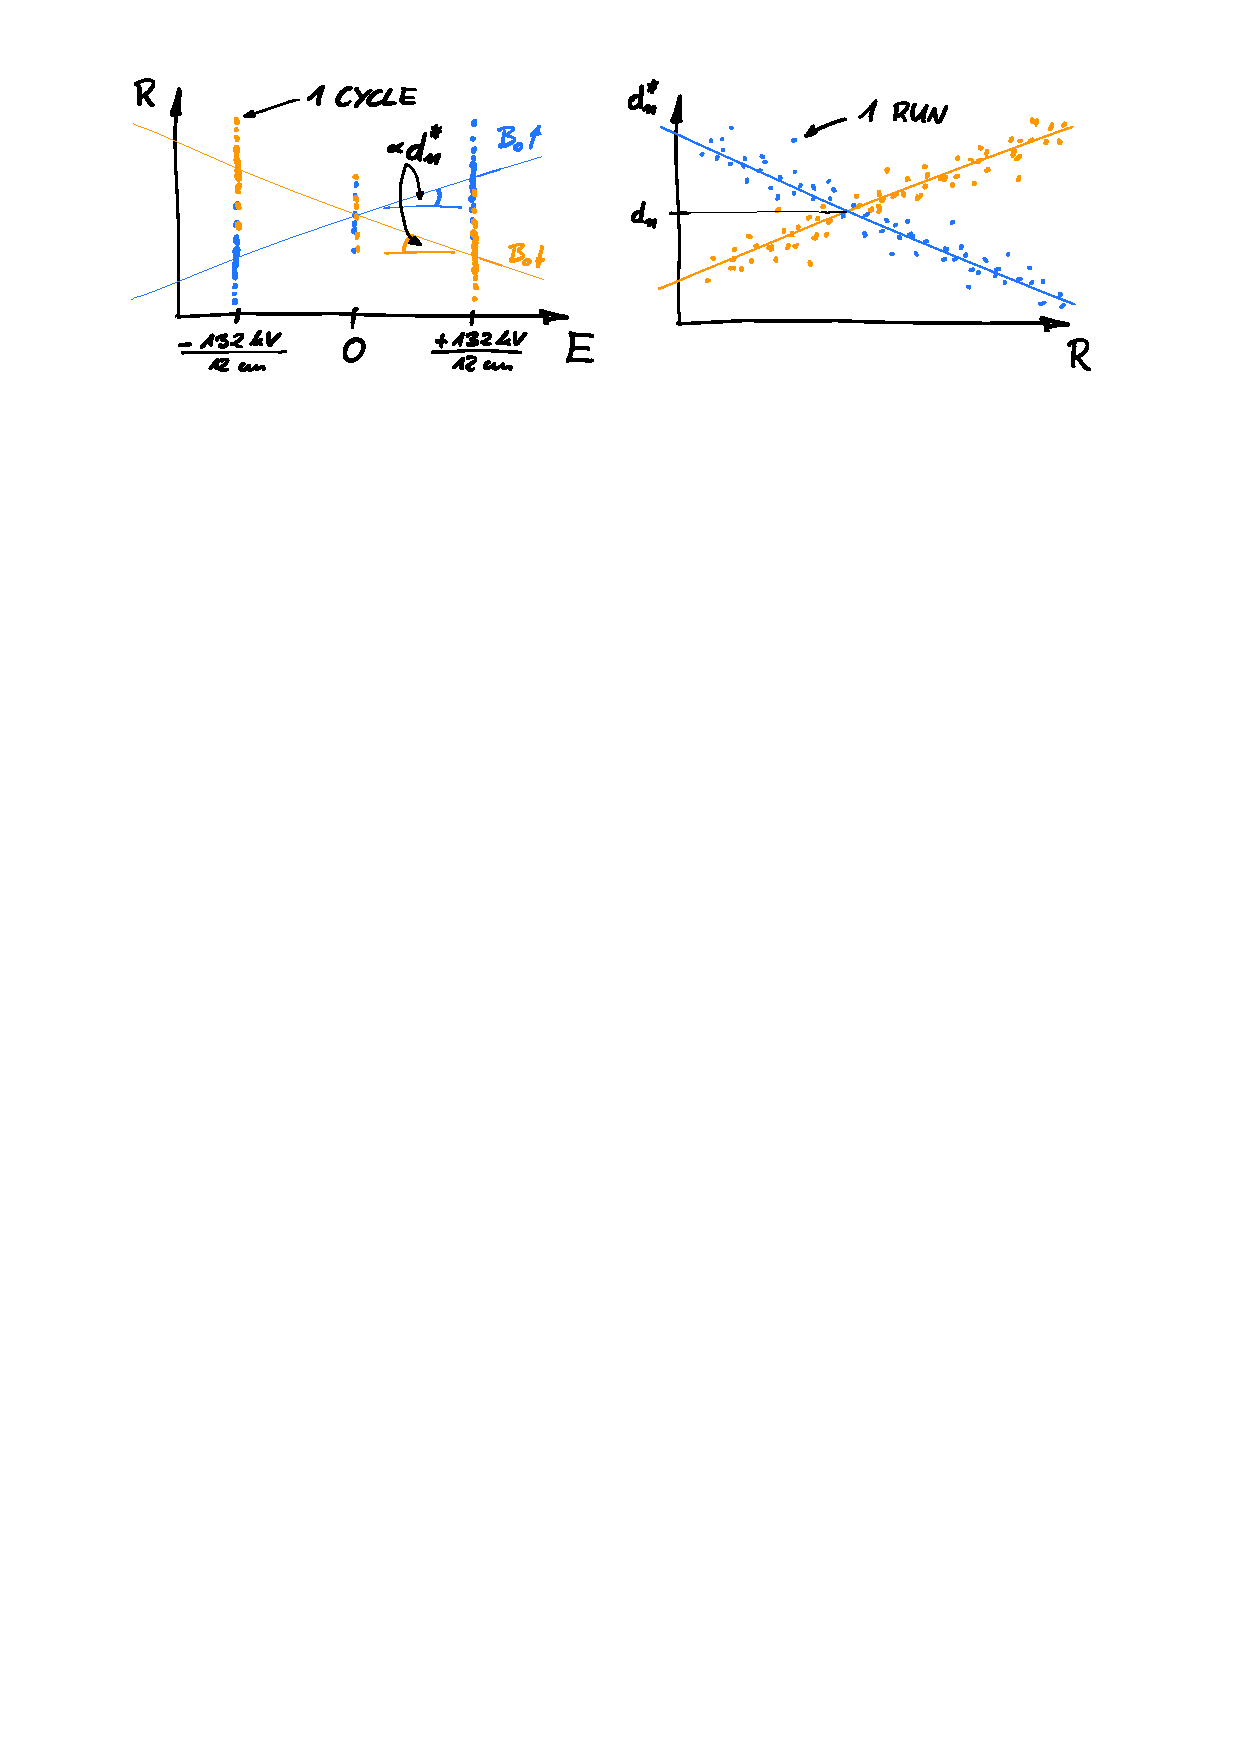
\includegraphics[width=0.9\linewidth]{gfx/nEDMatPSI/crossing_lines.pdf}
  \caption{The crossing lines in the nEDM estimation. Left: For each sequence, data taken in one magnetic field configuration, $d_n^*$ is estimated as the slope of a linear regression of $R$ vs. $E$ (Eq.\,\ref{eq:Rdefinition}). The two lines correspond to the parallel and anti-parallel configurations of the magnetic and electric fields. The $d_n^*$ are tainted by a systematic effect proportional to the gradient. Right: a linear regression is done on $d_n^*$ vs. $R$, $R$ being an estimate of the gradient. The crossing point of the two lines, one for the magnetic field pointing upwards, one for downwards, is the estimate of $d_n$ at zero gradient, so free from the gradient-proportional systematic effect.}
  \label{fig:crossing_lines}
\end{figure}

Those estimates, however, still contained a large contribution of a systematic effect (hence the star). As a result of a conspiracy between radial magnetic field components and rotating magnetic components arising from the Lorentz transformation of the large electric field into the rest frame of the mercury atoms, a frequency shift proportional to the applied electric field was observed, mimicking the effect of a non-zero electric dipole moment of the neutron, a false EDM. This effect is, however, directly proportional to the gradient of the applied vertical magnetic field $\partial_z B_z$, and reverses with the sign of the applied magnetic field. The false EDM effect has been analysed in more detail in \cite{Pendlebury2004,PhysRevA.71.032104,PhysRevA.73.014101} and a direct measurement of this effect was made in~\cite{Afach2015falseEDM}.

The solution was to operate in different gradients and then interpolate to the effect-free zero gradient. Every few hundred cycles a different gradient (up to \SI{60}{\pico\tesla\per\centi\meter}) was set.
%We set the magnetic configuration (homogenise the field, maybe mention the variometer method), apply a gradient (one of i don't remember how many), calibrate the Cs magnetometers (marginnote why) and measure continuously cycle after cycle in this configuration.
% We call a set of data taken in one configuration of the magnetic field a \emph{sequence}.
Finally, a for each direction of the magnetic field, a linear regression $d_n^*$ vs $R$, $R$ itself being an estimate of the gradient, was performed (Fig.\,\ref{fig:crossing_lines}). The vertical position of the intersection of the two lines corresponded to the $d_n$ measured at zero gradient, free from this systematic effect.

% In the nEDM experiment at PSI data taking is divided into \emph{runs}. A single \emph{run} is carried out automatically with, in most cases, no human intervention. The machine cycles through the working points by itself. Also the charging of the electrodes creating the electric field is automatised. In between \emph{runs} manual interference happens, most importantly the magnetic field vertical gradient is altered.

\marginpar{The blinding mimicked an nEDM signal by changing the logged detector mark for around one, on average, neutron count. The directon of the change depended on the electric field.}
On top of that, in order to mitigate the bias due to the human factor, the nEDM experiment implemented data blinding. The data was artificially altered in a way that mimicked a non-zero neutron electric dipole moment, big enough to be visible in the data. The exact offset value is secret and would be revealed only after the analysis was complete.

In this short description we only scratched the surface of the quite complex experiment. We discussed only those elements necessary for understanding the original work presented in the next chapters. More details can be found in the following references:~\cite{Zenner2013,Afach2015falseEDM,Afach2015,Afach2014magmoment,FertlThesis,Komposch2017}.











% Description of the experimental setup and the measurement procedure.

% \subsection{The Sussex-RAL-ILL Room Temperature Neutron Electric Dipole Moment Experiment}
% \note{NA: this subsection is still a very early draft, I know there are still formatting issues and blanks}

% \note{This first bit is paraphrased from C.A. Baker et al., Apparatus for Measurement of the Electric Dipole Moment of the Neutron using a Cohabiting Atomic-Mercury Magnetometer}

% \note{MR: This should probably be made much shorter.}

% Most experiments to measure the static electric dipole moment of the neutron use magnetic resonance techniques to observe the Larmor precession of free neutrons in parallel and antiparallel magnetic and electric fields. The Hamiltonian of an uncharged spin $1/2$ particle in an electric and a magnetic field is:
% \begin{equation}
% H = - 2\vec{S} \cdot (\mu \vec{B} + d \vec{E})
% \end{equation}
% In the case of parallel and antiparallel magnetic and electric fields, this gives a precession frequency of:
% \begin{equation}
% h\nu = -2\mu B \mp 2dE
% \end{equation}
% In the presence of a non-zero EDM, when the direction of the applied electric field is reversed relative to the magnetic field we expect a shift in the precession frequency of
% \begin{equation}
% \delta \nu _0 = −\frac{4d_n E_0}{h} .
% \end{equation}
% In the Sussex-RAL-ILL Room Temperature experiment, polarised ultracold neutrons produced at the fundamental physics beamline at the ILL high flux reactor were stored in a material bottle (a cylinder of diameter 235mm and height 120mm), wherein their precession frequency in parallel and antiparallel combinations of electric and magnetic fields was measured using the Ramsey Technique. To combat drifts in the magnitude of the applied magnetic field, a cohabiting magnetometer of atomic $^{199}$Hg was used, and analysis was done by considering the ratio of neutron and mercury precession frequencies, “$R$”.

% Each measurement sequence (“cycle”) consisted of a filling period, a first $\pi/2$ pulse to rotate the neutron spins into the horizontal plane, a 130s period of free precession, a second $\pi/2$ pulse to project the spins onto the z axis, and an emptying period where the number of spin-up and spin-down neutrons were counted. The precession of the mercury during the free precession period was measured by observing the modulation of the absorption of light from a mercury discharge lamp \note{is it actually a discharge lamp?}. Each cycle lasted in total x minutes. Many cycles were taken at each fixed magnetic field configuration over the course of between 1 and 73 hours (a “run”), while the direction of the applied electric field was reversed every 20 cycles. From each run a value of the neutron to mercury frequency ratio $R$ was extracted, as well as a value of the apparent EDM.

% As a result of a conspiracy between radial magnetic field components and rotating magnetic components arising from the Lorentz transformation of the large applied electric field into the rest frame of the mercury atoms, a frequency shift proportional to the applied electric field was observed, mimicking the effect of a non-zero electric dipole moment of the neutron --- a “false EDM”. This effect is, however, directly proportional to the gradient of the applied vertical magnetic field dBz/dz, and reverses with the sign of the applied magnetic field. The false EDM effect has been analysed in more detail in \note{cite false edm paper(s)} and a direct measurement of this effect was made in \note{cite false edm measurement}.

% As the ILL experiment had no direct measurement of the vertical gradient, the measurement of the neutron to mercury frequency ratio was instead used as a proxy. Due to the extremely low energy of the ultracold neutron population, the centre of mass of the neutron population sags a little below the centre of the precession chamber. The relatively hot population of mercury atoms does not suffer from this effect, so there is an effective height difference $\Delta h \approx 3.7 \mathrm{mm}$ between the neutron and mercury populations. Thus, the ratio of neutron to mercury frequencies depends (to first order) on the vertical gradient like: \note{MR: We might want to get rid of the stacked fraction for clarity.}
% \begin{equation}
%   R = R_0 \left( 1 + \Delta h  \frac{\frac{\mathrm{d}B_z}{\mathrm{d}z}}{B_{0}} \right).
%   \label{eq:R}
% \end{equation}
% This frequency shift does not uniformly affect the entire neutron population: the effect is much greater for the lowest energy neutrons which have a lower centre of mass. This causes a departure from the linear relation above; however, in the low vertical gradient regime ($\lesssim 30 \mathrm{pT/cm}$) in which most of the data was taken, the effect is almost exactly linear. This effect is described more thoroughly in [cite grav depol papers].

% To correct for these false EDMs in static EDM searches, the “crossing lines” procedure was adopted.  For each direction of the magnetic field, the measured EDM value was plotted against the measured neutron to mercury frequency ratio. Barring other systematic shifts, it is considered that the vertical gradient is zero where these lines cross. Other effects arising from transverse magnetic fields, the rotation of the earth and cause additional frequency shifts in the neutrons or in the cohabiting magnetometer, which can \note{PH: no it isn't -- there are still systematics from e.g. transverse fields, which can move the crossing point away from dB/dz=0, in addition to effects such as Earth's rotation that result in a vertical shift of the crossing point...]}, and therefore a measurement of the neutron electric dipole moment independent of the false EDM effect and of the neutron to mercury frequency ratio independent of the gravitational shift can be extracted. In the rest of the run-level analysis, we work with data where these false EDM effects have been subtracted. Further systematic effects shift the measured neutron to mercury frequency ratio or the measured EDM value, however these effects can be assumed to have been constant throughout the entire experimental measurement period, and so will not be further explored in this analysis. Systematic effects affecting the static analysis of the ILL experiment are explored in depth in [cite reanalysis] and [cite apparatus paper].

% \note{MR: Need to mention explicitly, that the average $d_n$ over a run is measured (though not exactly, it is only over the free precession periods), and this is how it is treated in the Monte Carlo simulations.}


% \section{nEDM @ PSI data taking scheme}
% The nEDM experiment at PSI probes the Ramsey resonance curve of ultra--cold neutrons (\emph{UCNs}). Its operation consists of subsequent \emph{cycles}, wherein an ensemble of polarised \emph{UCNs} undergoes a Ramsey cycle in a magnetic field. At the end the polarisation of the ensemble is measured. The measurement is performed in a controllable electric field, which takes up three values: parallel to the magnetic field, antiparallel to it and zero. The electric field configuration is altered every couple of tens of cycles.

% The Ramsey resonance curve of the neutrons is probed only in four \emph{working points}, as shown in Fig.\,\ref{fig:axions_working_points}. The points lie on the curve's steep slope. Thereby the resonance position is determined more precisely then it would should the curve be probed homogeneously or close to the resonance.

% \begin{figure}[bth]
%   \myfloatalign
%   \subfloat
%   [The \emph{working points} method. The plot depicts the measured neutron polarisation in function of the $pi/2$ pulses frequency. The frequencies are normalised by appropriate gyromagnetic ratios.]
%   {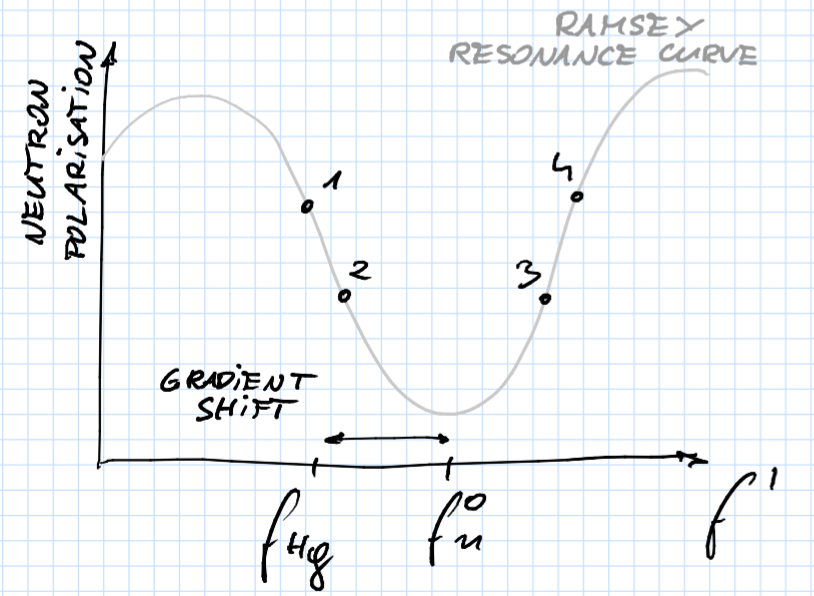
\includegraphics[width=.45\linewidth]{gfx/axions/data_taking_working_points}}
%   \quad
%   \subfloat
%   [The \emph{working points} are probed subsequently.]
%   {\label{fig:example-b}
%   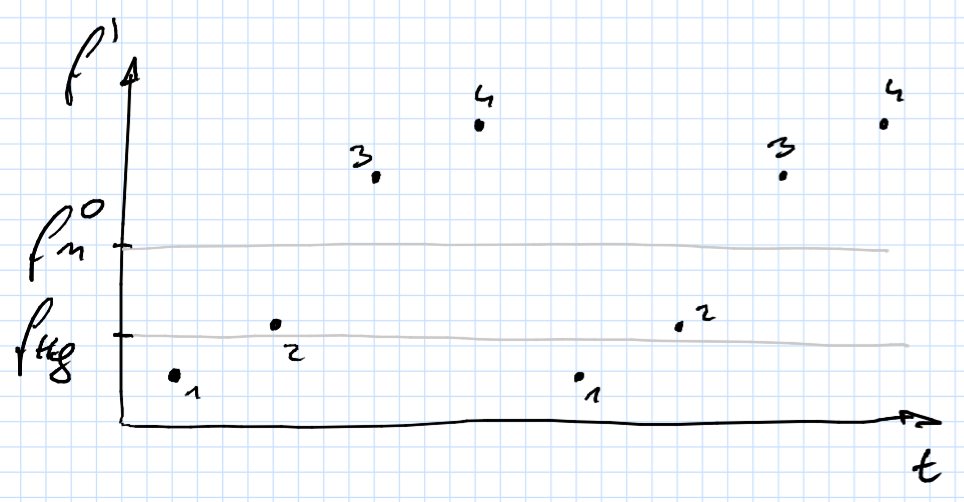
\includegraphics[width=.45\linewidth]{gfx/axions/data_taking_working_points_time}}
%   \caption{The principle of working points}
%   \label{fig:axions_working_points}
% \end{figure}

% The resonance frequency $f_n^{\,0}$ is determined with a fit of the resonance curve. Because the points are probed one after another, it is only possible after a set of data points, \emph{cycles}, have been measured. In order to extract the neutron precession frequency for each individual \emph{cycle}, one assumes that the only parameter of the resonance curve that varies on a cycle--to--cycle basis is the position of the resonance. With this assumption the shape of the curve, fitted to the whole set of \emph{cycles}, is used to calculate back the resonant frequency in each \emph{cycle} of the set.

% Together with the UCNs there is a polarised $^{199}$Hg gas precessing. Its precession is monitored with light, allowing for direct determination of the $^{199}$Hg Larmor frequecy and thus the magnetic field strength. In order to cancel the first-order magnetic field changes one looks at the value:
% \begin{equation}
%   R := f_n / f_{Hg} \ .
% \end{equation}
% However, the UCNs are cold enough to have their centre of mass shifted downwards a few centimeters by the gravity. The $^{199}$Hg gas, being much hotter then the UCNs, fills the precession volume homogeneously. In a presence of a vertical magnetic field gradient this causes the two species to see different magnetic fields.

% In the nEDM experiment at PSI data taking is divided into \emph{runs}. A single \emph{run} is carried out automatically with, in most cases, no human intervention. The machine cycles through the working points by itself. Also the charging of the electrodes creating the electric field is automatised. In between \emph{runs} manual interference happens, most importantly the magnetic field vertical gradient is altered.

% In order to mitigate the bias due to the human factor, the nEDM experiment implements \emph{data blinding}. The data is artificially altered in a way that mimics a non--zero neutron electric dipole moment, big enough to be visible in the data. The exact value is secret and will be revealed only after the analysis is complete.


% -------------------------------------------------------
% SFC DESIGN
% -------------------------------------------------------
\ctparttext{
Stability of the magnetic field is a major challenge in measurements of the electric dipole moment of the neutron.
An active magnetic shielding system had been succesfully used already in the nEDM experiment.
This part begins with a discussion of the principles of active magnetic shielding and a description of the nEDM's system.

Spatial constraints made the design of coils for an n2EDM active shield challenging.
This motivated the development of a new method of magnetic field coil design, which is part of this work.

Further, a prototype of an active magnetic shield featuring coils designed with the new method is described.
The system had an unprecedentedly large useful volume.
It constructively showed, that an active magnetic shield for the n2EDM experiment could be built.

Finally, a magnetic field mapping device is presented.
It was used to characterise the magnetic field on the n2EDM site, providing crucial input to the design of an active shield.
    
The developments described in Part II laid the foundation for an active magnetic shield for the n2EDM experiment, which would reduce the tens-of-microteslas variations down to just a few.
}
\part{Active Magnetic Shielding}
\chapter{The nEDM active magnetic shielding}

\label{ch:nedm_sfc}
In this chapter the principle of an active magnetic shielding is explained, followed by a description of the system of the PSI nEDM experiment. The matrix-based feedback algorithm and the properties of the matrix are discussed. Finally, the challenges for the design of a next-generation system for the n2EDM experiment at PSI are stated.




\section{The principle of active magnetic shielding}
Passive methods of shielding the magnetic field, like mu-metal shields, rely on magnetic properties of materials. In contrast, in active methods the disturbances are first detected, processed and then counteracted. It is not unlike the recently popular active-noise-cancellation headphones. Standard ones provide only passive damping of the ambient noise by covering the ears. Active headphones additionally feature microphones that resolve the profile of incoming sound, which is then inverted and emitted from the speakers. The two waveforms, when overlaid, cancel.

\begin{figure}
  \centering
  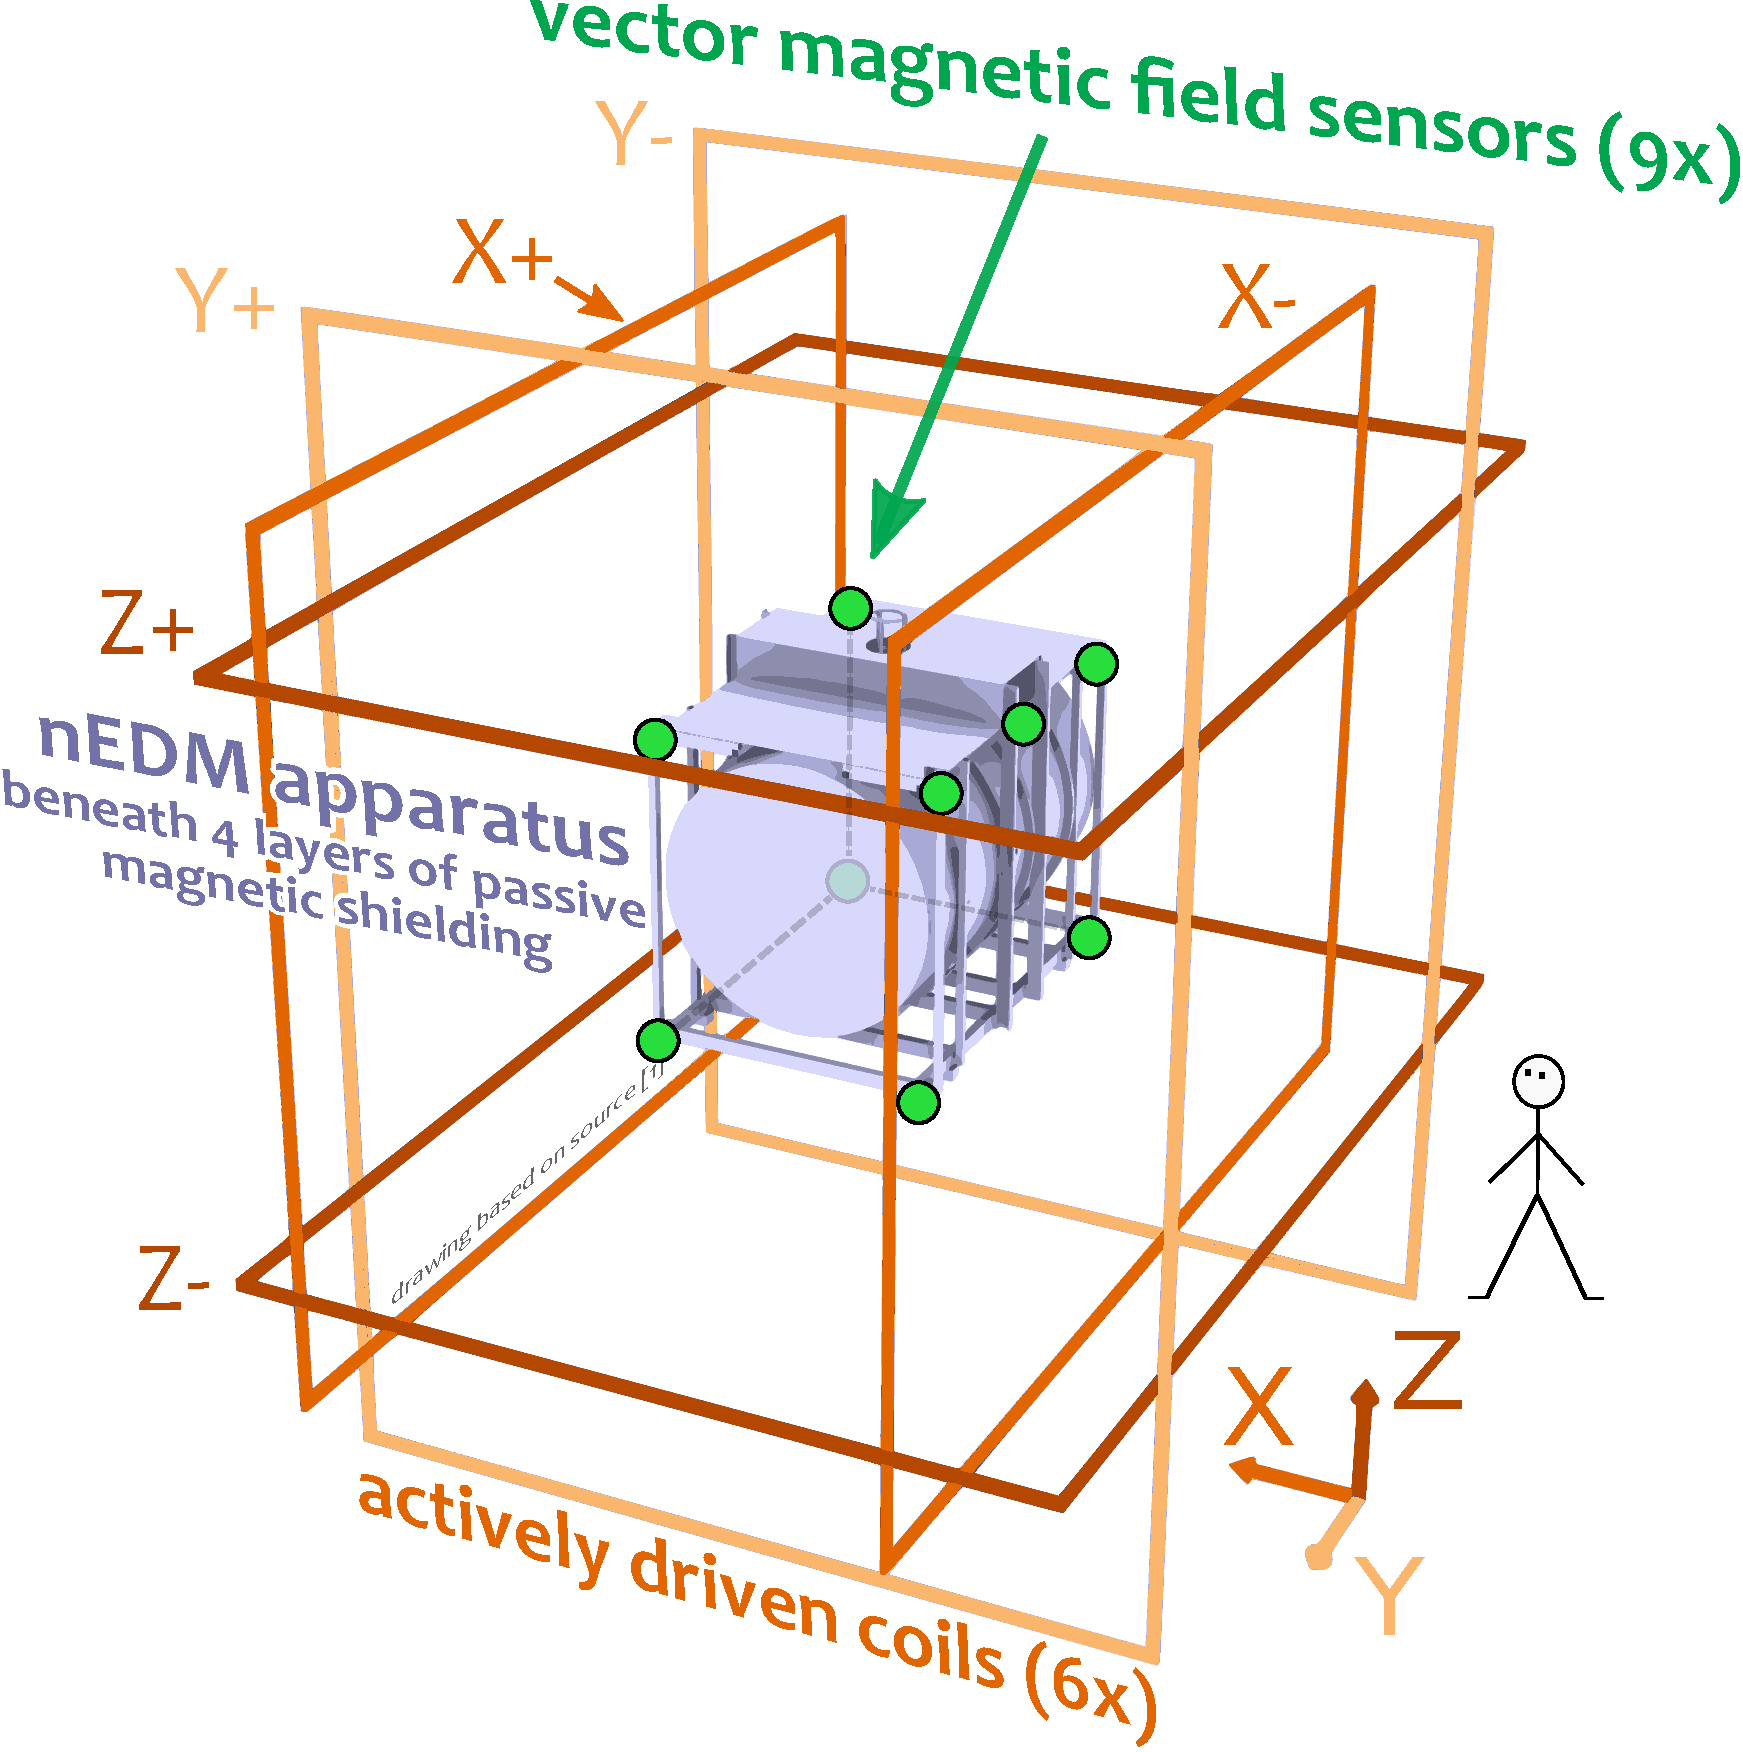
\includegraphics[width=0.8\linewidth]{gfx/nEDM_SFC/SFC_scheme.pdf}
  \caption{The nEDM at PSI active magnetic shield (SFC). The experiment, in violet, was in the middle, with nine 3-axis magnetic field sensors, depicted as green circles, attached to it. Everything was encircled by six coils (orange). Adapted from~\cite{Franke2013}.}\label{fig:sfc-scheme}
\end{figure}

Active magnetic shields follow the same principle. A volume, often called the fiducial volume, is encircled by coils. Within the volume magnetic field sensors are distributed. It is schematically presented in Fig.\,\ref{fig:sfc-scheme}, taking the PSI nEDM experiment's system as an example. The fiducial volume is filled with the violet structure in the middle (the passive shield). The green dots depict the magnetic field sensors. Around there are three orthogonal Helmholtz-like pairs of coils, depicted in shades of orange. The sensors detect the variations of the magnetic field, an appropriate counteraction is calculated and currents are applied to the coils.

\marginpar{Shielding factor, measured in \si[detect-all=true]{\decibel} is a tenth of the logarithm of the ratio of the power of the magnetic field as if it were not compensated to the compensated one.}
Active shields do not substitute passive ones.
The shielding factor of passive shields degrades for frequencies slower than \SIrange[range-phrase = --]{1}{10}{\hertz}~\cite{Brake1991,PTBroom}.
% The loss in the shielding factor can be as much as \SI{70}{\decibel} (three orders of magnitude in amplitude of the field).
At the same time active systems perform best at DC and reach up to the kilohertz regime.
The combination of the two shielding methods provides a stable magnetic field over the whole range of frequencies~\cite{Brake1991,Kelha1982,PTBroom,Voigt2013}.

Since the 1980s numerous active shields have been built~\cite{Kelha1982,Brake1991,Spemann2003,Brys2005,Kobayashi2012,Voigt2013,Afach2014}. The applications span from ion beams, through bio-magnetism, all the way to nEDM measurements, in particular the one conducted at PSI\@.

\marginpar{There was an inside joke that SFC really stands for SULTAN Field Compensation, SULTAN having been the magnet with by far the strongest influence on the magnetic field.}
\section{The nEDM at PSI SFC system}
The construction of an active shield for the nEDM measurement at PSI, called the SFC (Surrounding Field Compensation) system,
was a part of Beatrice Franke's PhD thesis~\cite{Franke2013}, later also published~\cite{Afach2014}.

% In this section the SFC system is presented, fo
% In the beginning of this chapter the most important information about the SFC system is presented, followed by a few new insights. This serves as an introduction to the original developments, to which the remaining three chapters of part II are dedicated.

The distinct feature of the PSI's SFC system was the use of a feedback matrix.
\marginpar{A matrix-based feedback was first proposed by~\cite{RetaHernandez1998}. As their proposed system did not include $\mu$-metal, they could calculate the matrix analytically.}
Consider a single coil of any shape in air. For every point in space, and for every spatial component, the magnetic field is directly proportional to the current in the coil. The SFC system had six coils and measured the field in nine points, three spatial components in each. In total there were $6 \times 27 = 162$ proportionality constants, which were gathered in the feedback matrix $M$. The matrix $M$ is a property of the active compensation system, more precisely of the geometry of the coils and sensors. It could have been calculated analytically, if not for the mu-metal shield. Ferromagnetic materials distort the magnetic field around them.
Different to similar systems~\cite{Kelha1982,Brake1991,Spemann2003,Brys2005,Kobayashi2012,Voigt2013}, which used independent feedback for each coil, the SFC system at PSI used the matrix $M$ that mixes all sensors and all coils. 
% The use of the matrix $M$ was what distinguished the PSI's SFC system from other systems~\cite{Kelha1982,Brake1991,Spemann2003,Brys2005,Kobayashi2012,Voigt2013}, which used either one component of a sensor, or a weighted combination of several components, to control one coil.

\begin{figure}
  \centering
  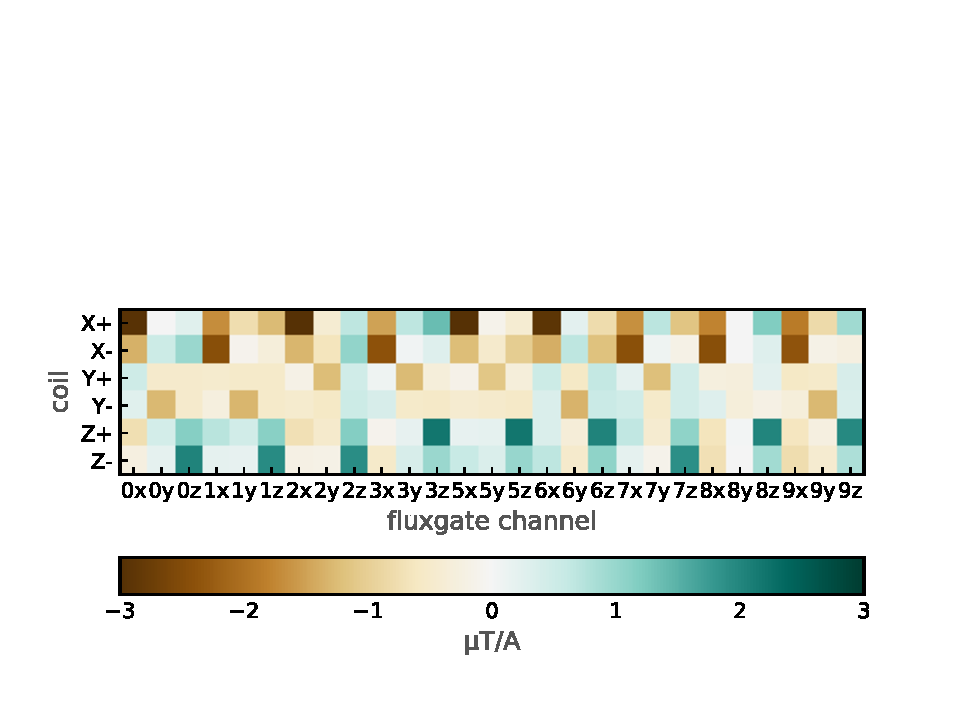
\includegraphics[width=.8\linewidth]{gfx/nEDM_SFC/nEDM_SFC_matrix.pdf}
  \caption{The SFC matrix measured by Franke on 2012--11--07~\cite{Franke2013}. For each coil (rows) and each channel of the magnetic field measurement (columns) the proportionality constant between the current in the coil and the field measured by the sensor is depicted. The coils and the sensors are labelled as in Fig.\,\ref{fig:sfc-scheme}.}\label{fig:nEDM_SFC_matrix}
\end{figure}

To measure the matrix the following procedure was used: A current in one coil was scanned in steps over the whole available range, while the field change was measured with the sensors. Then for each sensor, and each spatial component, a linear regression was performed. The slope corresponded to the proportionality constant, an element of the matrix $M$. The procedure was repeated for all coils. The matrix measured by Franke is depicted in Fig.\,\ref{fig:nEDM_SFC_matrix}.




\section{The feedback algorithm}
The PSI's SFC system followed the established norm~\cite{Kelha1982,Brake1991,Spemann2003,Brys2005} and used a PID loop to control the currents. (PI in this particular case, the derivative term was not used.) The $j$th current in the $n$th iteration was~\cite{Franke2013}:
\begin{equation}
  \label{eq:old_SFC_feedback}
  I^n_j = I^0_j +
    \underbrace{ \alpha^\mathcal{P}_j \, \Delta I^n_j }_\text{proportional term} +
    \underbrace{ \alpha^\mathcal{I}_j \, \sum_m \Delta I^m_j }_\text{integral term} \ .
\end{equation}

% $\Delta I^n_j$ is the error value in the current space. It was obtained by using the error value in the field space (the difference of the measured and target fields) and transforming it into the current space with the pseudoinverse of the matrix~\cite{Franke2013}:
$\Delta I^n_j$ is the error value. It was obtained from the deviation of the measured and target field, $\Delta B^n_{k'}$ for the $k'$th sensor, by multiplying it by the pseudoinverse of the matrix $M$, denoted $M^\dagger$~\cite{Franke2013}:
\begin{equation}
  \Delta I^n_j = \sum_{k'} M^\dagger_{jk'} \, \Delta B^n_{k'} \ .
\end{equation}

\marginpar{The SFC system, when started, was static. Then the currents could be changed manually to achieve a desired field (or chosen from a predefined set). Then the system was switched to the dynamic mode~\cite{Franke2013}.}
Besides the proportional and integral terms, the feedback formula also included the $I^0_j$ term. It may seem puzzling to give such a big of a role to particular currents that had happened to be there at the zeroth iteration. The reason behind this choice was a particular property of the SFC system: the target field was always the one measured at the moment of switching the system from the dynamic mode (feedback running) to the static one (static current output).
At that moment the error value was zero, and so was the integral term, so, according to the Eq.\,\ref{eq:old_SFC_feedback}, the output currents would immediately have switched to zero. In result the system would violently destabilise. The additional term $I^0_j$ prevented that from happening.

Here we conclude the brief description of the system and proceed to present original insights of the author.




\section{Interpretation of the feedback matrix}
There is a fundamental meaning behind the matrix $M$. The currents in the six coils can be gathered into a vector $\mathbb{I}$ in a space we call the \emph{current space}. Similarly, the 27 readouts of the magnetic field can be gathered into a vector $\mathbb{B}$ in the \emph{field space}. Then, the matrix $M$ provides the transition from the current into the field space. In particular, we have:
\begin{equation}
  \mathbb{B} = M \mathbb{I} + \mathbb{B}_\text{offset} \ .
\end{equation}
\marginpar{Finding the pseudoinverse of a matrix $A$ is equivalent to finding least-squares solution of a system of linear equations described by the matrix $A$ (although computationally more complex).}
Which is read: The measured values are a linear combination of the currents in the coils plus the ambient field.
The other direction, from the field to the current space, cannot be done exactly. Nevertheless, the optimal, in the least-squares sense, transition can be done with the use of the Moore-Penrose inverse (pseudoinverse) of the matrix $M$, denoted $M^\dagger$~\cite{penrose_1955}.
In other words, the matrix $M$ tells us what field, as measured by the sensors, a given set of currents will produce. The matrix $M^\dagger$ tells us, what currents to apply to best approximate a given field.




\section{The spectrum of the feedback matrix}
\label{sec:nedm_sfc_matrix}
The feedback matrix used during the data taking of the nEDM PSI experiment at PSI (2014--17) was the one measured by Franke (Fig.\,\ref{fig:nEDM_SFC_matrix}). The inverse of the matrix was regularised~\cite{Franke2013}. Let us now elaborate on regularisation.
% While it has been thoroughly discussed how to do the regularisation, the question of why was it needed at all was neither posed nor answered.

The feedback matrix represents coefficients in a system of linear equations that need to be solved in order to make the optimal transition from the field to the current space.
As the system of equations is over-determined, the best solution is found by the least-squares.
This is equivalent to calculating the pseudoinverse matrix. A solution can be found reliably if the system is well-defined, i.e.\ the least-squares well is steep in every direction in the parameter space.
If the well stretches, like a valley, in some directions, the solution is not globally well-defined.
Still, it may be defined up to a parameter, the one pointing along the direction of the valley.
We then speak of an ill-defined set of equations, or an ill-defined matrix.
Regularisation helps an ill-defined problem to become better defined, at the cost of the solution having larger sum of the residuals squared.

The \emph{Singular Value Decomposition} (SVD) of a real matrix $M$ is
\begin{equation}
  M = U S V^T \ , 
\end{equation}
where $U$ and $V$ are unitary, and $S$ is diagonal~\cite{Golub1965}.
The singular values lie on the diagonal of $S$, which is called the \emph{spectrum}.

\begin{figure}
  \centering
  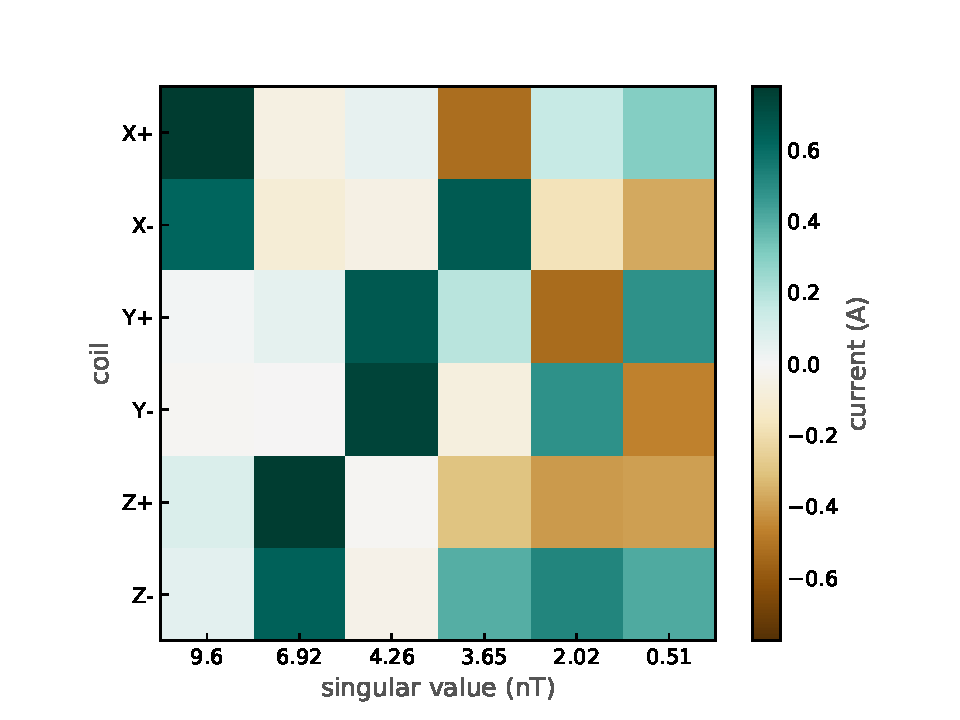
\includegraphics[width=.8\linewidth]{gfx/nEDM_SFC/coil-singular_vectors_of_the_nEDM_SFC_matrix.pdf}
  \caption{The coil-singular values of the SFC matrix.
  Columns correspond to singular combinations of the coils (labeled as in Fig.\,\ref{fig:sfc-scheme}).
  For each column the corresponding singular value is indicated.}\label{fig:nEDM_SFC_svd}
\end{figure}

The \emph{condition number} of a matrix is defined as a ratio of the extreme values of its spectrum~\cite{Regression}.
For a matrix with a flat spectrum, all singular values equal, the condition number is one.
A set of linear equations represented by such a matrix is well defined.
The more extreme values differ, the higher the condition number and the worse defined the problem is.
The effect is, that the noise in the original matrix becomes amplified by the condition number in the pseudoinverse. Figure~\ref{fig:nEDM_SFC_svd} presents the spectrum of the PSI's SFC feedback matrix.
The condition number is $9.6 / 0.51 = 18.2$.
A factor of 18 amplification of noise points to why the regularisation was necessary.

It is interesting to ask \emph{why} the system had an ill-defined feedback matrix.
A very small singular value means that there exists a coil, or a combination thereof, which has about 18 times smaller influence on the field then other ones.
In Fig.\,\ref{fig:nEDM_SFC_svd} the columns are the singular values with their corresponding coil-vectors.
The first three, starting from the left, are easiest to interpret.
Each of them is a pair of coils configured as Helmholtz-pair with roughly the same current, producing a homogeneous field in each of the spatial directions.
%The smaller singular value, or the effect on the field, in the Y direction is explained by the fact that this is the longitudinal axis of the μ-metal cylinder.
The last column has also a clear interpretation: it corresponds to all pairs configured as anti-Helmholtz---currents flowing in the opposite directions in each pair.
The magnetic field that was created by such a configuration was complicated and high-order.
The fact that this combination has so little influence on the measured field means that it hardly changes any solution for currents when added to it.
It spans a valley in the parameter space in the least-squares problem.
If not regularised, a small change in the measured field would cause a large change in the currents along the valley.
Rapid oscillations in this direction would render the system unstable.

An important observation is that the feedback matrix is defined solely by the configuration of the coils, sensors and ferromagnetic materials.
It follows that already at the design stage one can, and should, take care about the definiteness of the system.




\section{Design challenges for n2EDM}
\label{sec:n2EDM_challenges}
There was relatively a lot of space available around the passive magnetic shield of the nEDM experiment at PSI (see Fig.\,\ref{fig:sfc-scheme}).
The SFC system exploited that space by making the coils much larger than the shield.
However, the successor experiment, n2EDM, was going to have a much larger passive magnetic shield.
Spatial constraints were a major concern in the design of coils of a new active shield.

 Assume, that all there is to compensate are homogeneous fields.
 That is the zeroth order approximation concerning the space expansion of the magnetic field.
 To compensate them, a system needs to have coils that can produce a homogeneous field.
 Yet, the volume where the field of a coil system is homogeneous is limited.
 For example, in a case of a Helmholtz pair, the (linear) size of the volume where the generated field is homogeneous on a \SI{2}{\percent} level is only around \num{0.4} that of the (linear) size of the coils.
 Increasing the relative size of the homogeneous volume requires more elaborate designs~\cite{Kirschvink1992}.
 When three Helmholtz pairs are used to compensate a homogeneous change, they only do so inside this limited volume.
 Outside, the field may even be more unstable, the extreme case being right next to the coils, where the field can get arbitrarily large.
 The situation is similar for any type of field: an active shield can only stabilise the field in a limited volume.

\begin{figure}[tbh]
  \centering
  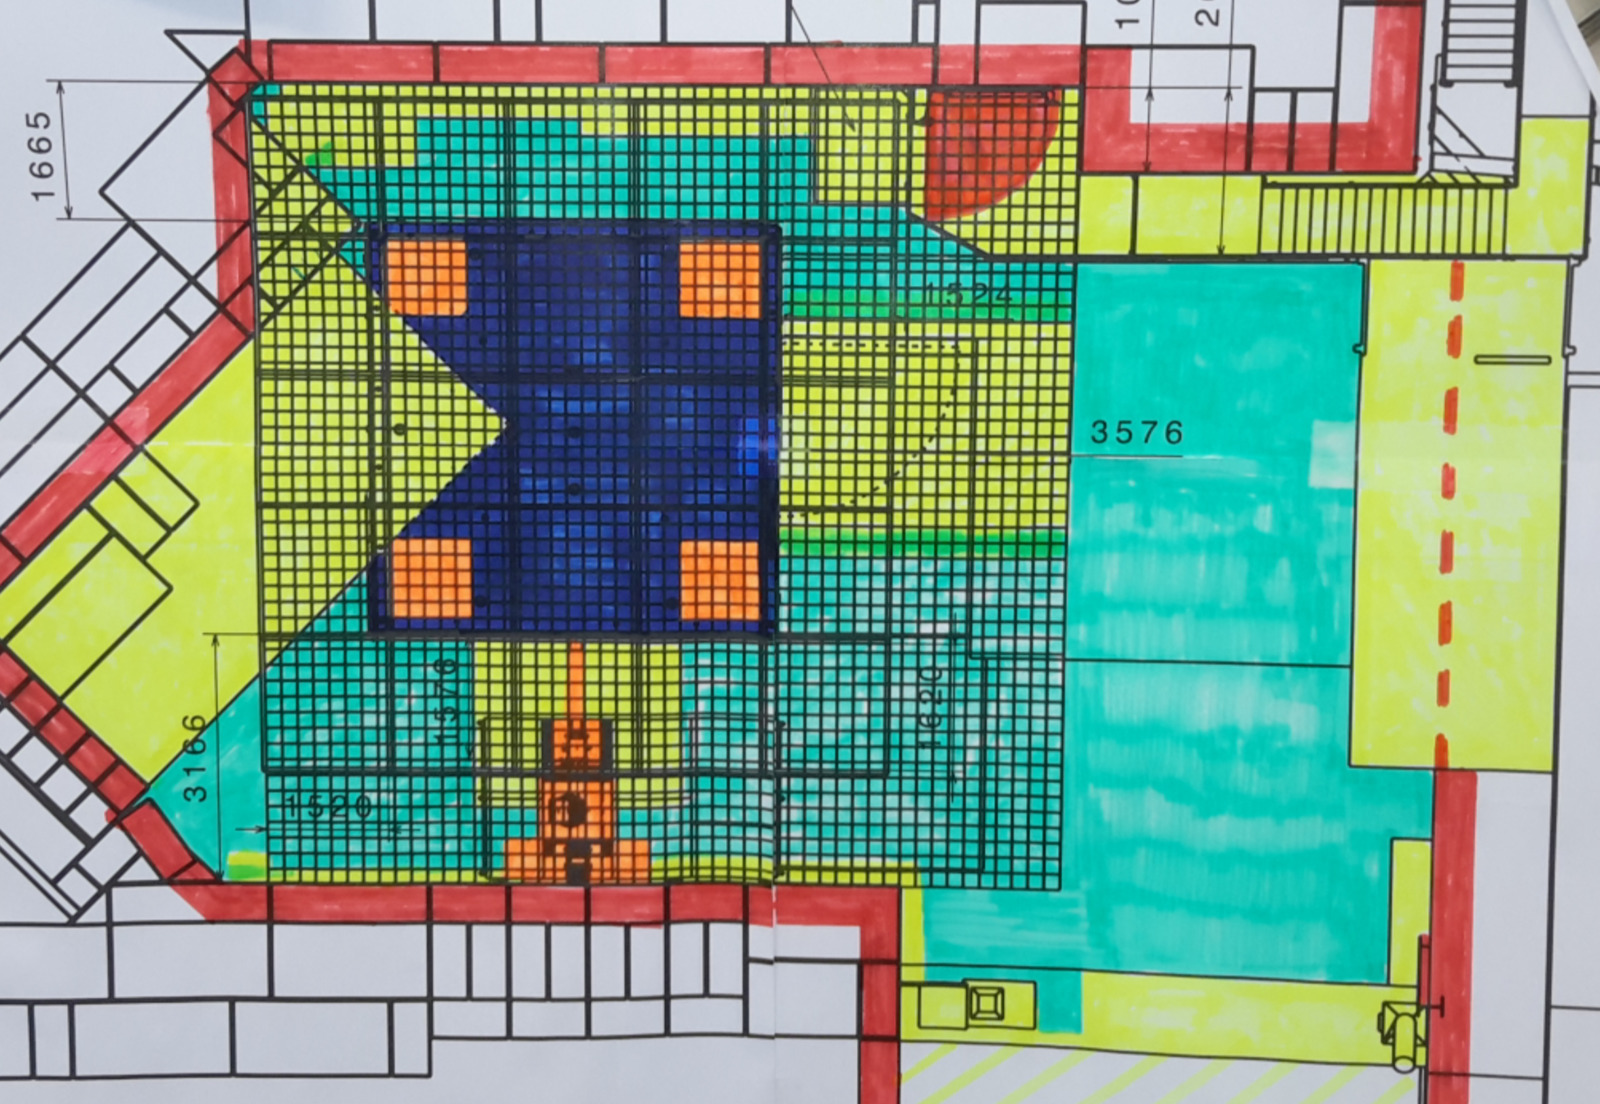
\includegraphics[width=\linewidth]{gfx/nEDM_SFC/n2EDM_SFC_situation.jpg}
  \caption{A plan by Michael Meier highlighting the potential conflicts between coils of an n2EDM active shield and other structures. The vicinity of the biological shielding (red) forced the coils to be designed relatively close to the magnetic shield (dark blue). Other bodies, like the support legs of the passive shield (orange), polarising magnet (orange) and an emergency exit from a nearby accelerator (red) gave additional constraints.}\label{fig:n2EDM_sfc_situational_plan}
\end{figure}

Figure~\ref{fig:n2EDM_sfc_situational_plan} depicts the major spatial constraints in the design of the n2EDM active shield.
Firstly, the passive shield was going to be \SI{5}{\metre} large in each direction, with the available space being $\approx \SI{7.5}{\metre}$ (a ratio of \num{0.7}).
In nEDM the shield was around \SI{2}{\meter} and the SFC coils \SIrange[range-phrase = --, range-units=single]{6}{8}{\meter} (a ratio of around \num{0.3}).
Secondly, other bodies put additional constraints (Fig.\,\ref{fig:n2EDM_sfc_situational_plan}): support legs of the passive shield, the polarising magnet and an emergency exit from a nearby cyclotron.

For the design of the n2EDM active shield it was necessary to come up with coils that could produce such a field, that they are likely to compensate, and do that in the whole volume occupied by the shield. Unfortunately, because of spatial constraints no known design could be used~\cite{Turner1986,Wong1991,Turner1993,Crozier1993,Sanchez2007,Sanchez2009}. This, together with a concern about ensuring a low condition number of the system, called for an in-depth investigation into the geometry of the future system's coils, which led to the development of a new approach to magnetic field coils design---the topic of the next chapter.

% Some came from the experimental hall itself. For example an emergency exit from a nearby accelerator and a staircase leading to it (see Fig.\,\ref{fig:n2EDM_sfc_situational_plan}). Other constraints were due to higher-priority components of the experiment itself: legs on which the shield stands, the magnet used to polarise the neutrons, the neutron detection system, and the door of the magnetic shield.

% !TEX root = ../rawlik-phd-thesis.tex
\chapter{Coil design}
\label{ch:coil_design}

In this chapter we present a new method to design a coil producing an arbitrarily shaped magnetic field. We achieve that by restricting the path of the coil's wires to a regular grid. The solution is then found by a simple least squares minimum. We discuss practical applications, in particular in an active magnetic shielding.




\section{Introduction}
\marginpar{This chapter is largely adapted from the author's publication CITE WHEN AVAILABLE}
How to design a coil, or more generally, an arrangement of coils, producing a desired magnetic field? In its simplest form this is a textbook problem (e.g.\ ex. 6.55 and 6.62 in Ref.\,\cite{Purcell}). Yet, in a general setting it is surprisingly hard and the solutions, how the wires making up the coils should be laid, complicated. The most widespread application of high-performance coils is Magnetic Resonance Imaging (MRI), where gradient coils give the possibility to produce spatial images. Already in the 1980's elaborate methods of MRI coil design have been developed. They range from optimizing positions of discrete windings, where the use is made of symmetries specific to MRI, to analytical methods yielding surface current density, which is then discretised. A general overview can be found in Ref.\,\cite{Turner1993}. Another field known for complex, precise coils is plasma confinement, in particular stellarators~\cite{Beidler1990}. There analytical solutions for the surface current density find their use, too.

Here, a new method is presented, that may not be competitive in terms of precision, but is distinct in its simplicity. Also when it comes to construction of its designs. It relies on an algebraic representation of the problem, where coil design is simplified to a simple linear least squares problem. In the method the coils are restricted to a user-defined mesh, making it easy to deal with spatial constraints.

The discussion is based on textbook linear algebra techniques, notably solving an over-determined system of linear equations, thoroughly discussed e.g.\ in Ref.\,\cite{Anton}. The main physics problem, calculating the magnetic field of coils composed of straight wire segments, is briefly discussed here. More in-depth discussions can be found, for example, in Ref.\,\cite{Griffith}. Furthermore, the implementation of the discussed problems, including examples, has been published and open-sourced~\cite{Coilsjlcode}.

We begin with a description of our model for a restricted two-dimensional case and generalize it to three dimensions. We then present how the model is used to design a coil, based on an example. Further we discuss possibilities of simplifying the solution. Another section is devoted to practical considerations, significant for the eventual construction. Finally, the application to active magnetic field shielding is considered.




\section{Coils as a linear space}
Consider all possible coils that can be constructed by laying a wire on a surface of a square. The possibilities are endless. Speaking more precisely, as the wires may be shifted by arbitrarily small distances, as they overlap and cross, the problem has inherently an infinite number of degrees of freedom. Here, an algebraic representation that reduces the number of degrees of freedom to just a few is proposed.

Start with a straight, finite wire segment spanned between points $\mathbf{x}_1$ and $\mathbf{x}_2$ (represented by vectors in an arbitrary coordinate system) and carrying current $I$, as depicted in Fig.\,\ref{fig:biot-savart}. The magnetic field it produces in the point $\mathbf{p}$ can be calculated with the use of the Biot-Savart law. Consider the vector normal to the wire through the point $\mathbf{p}$:
\begin{equation}
  \boldsymbol{\uprho} = (\mathbf{x}_1 - \mathbf{p}) - \left( \left( \mathbf{x}_1 - \mathbf{p} \right) \cdot \mathbf{n} \right)\mathbf{n} \ ,
\end{equation}
where $\mathbf{n}$ is a unit vector in the direction $\mathbf{x}_2 -\mathbf{x}_1$. The magnitude of the magnetic field in point $\mathbf{p}$ is then~\cite{Griffith}:
\begin{equation}
  \label{eq:biot_savart}
  B = \frac{\mu_0 I}{4 \pi \rho} \, \left| \sin \alpha_2 + s\, \sin \alpha_1 \right| \ ,
\end{equation}
where the angles $\alpha_i$ are not directed
\begin{equation}
  \sin \alpha_i = \frac{ \left\lVert \left( \mathbf{x}_i - \mathbf{p} \right) \times \boldsymbol{\uprho} \right\rVert }{ (x_i  - p) \rho } \ ,
\end{equation}
and $s$ is $+1$ if $\boldsymbol{\uprho}$ points onto the wire segment (between points $\mathbf{x}_1$ and $\mathbf{x}_2$) and $-1$ otherwise:
\begin{equation}
  s = \mathrm{sgn}\left( \tfrac{1}{2} \left\lVert \mathbf{x}_2 - \mathbf{x}_1 \right\rVert -
  \left\lVert \mathbf{p} + \boldsymbol{\uprho} - \tfrac{1}{2} \left( \mathbf{x}_1 + \mathbf{x}_2 \right) \right\rVert \right)
\end{equation}
\marginpar{Another formulation, with better numerical properties close to the axis of the wire, can be found in Ref.\,\cite{Hanson2002}.}
The direction of the field is given by the right-hand principle:
\begin{equation}
  \mathbf{B} = \frac{B}{\rho} \boldsymbol{\rho} \times \mathbf{n}
\end{equation}
This formulation is independent of the coordinate system (coordinate-system dependent solutions can be found e.g.\ in Ref.\,\cite{Grivich2000}).

\begin{figure}
  \centering
  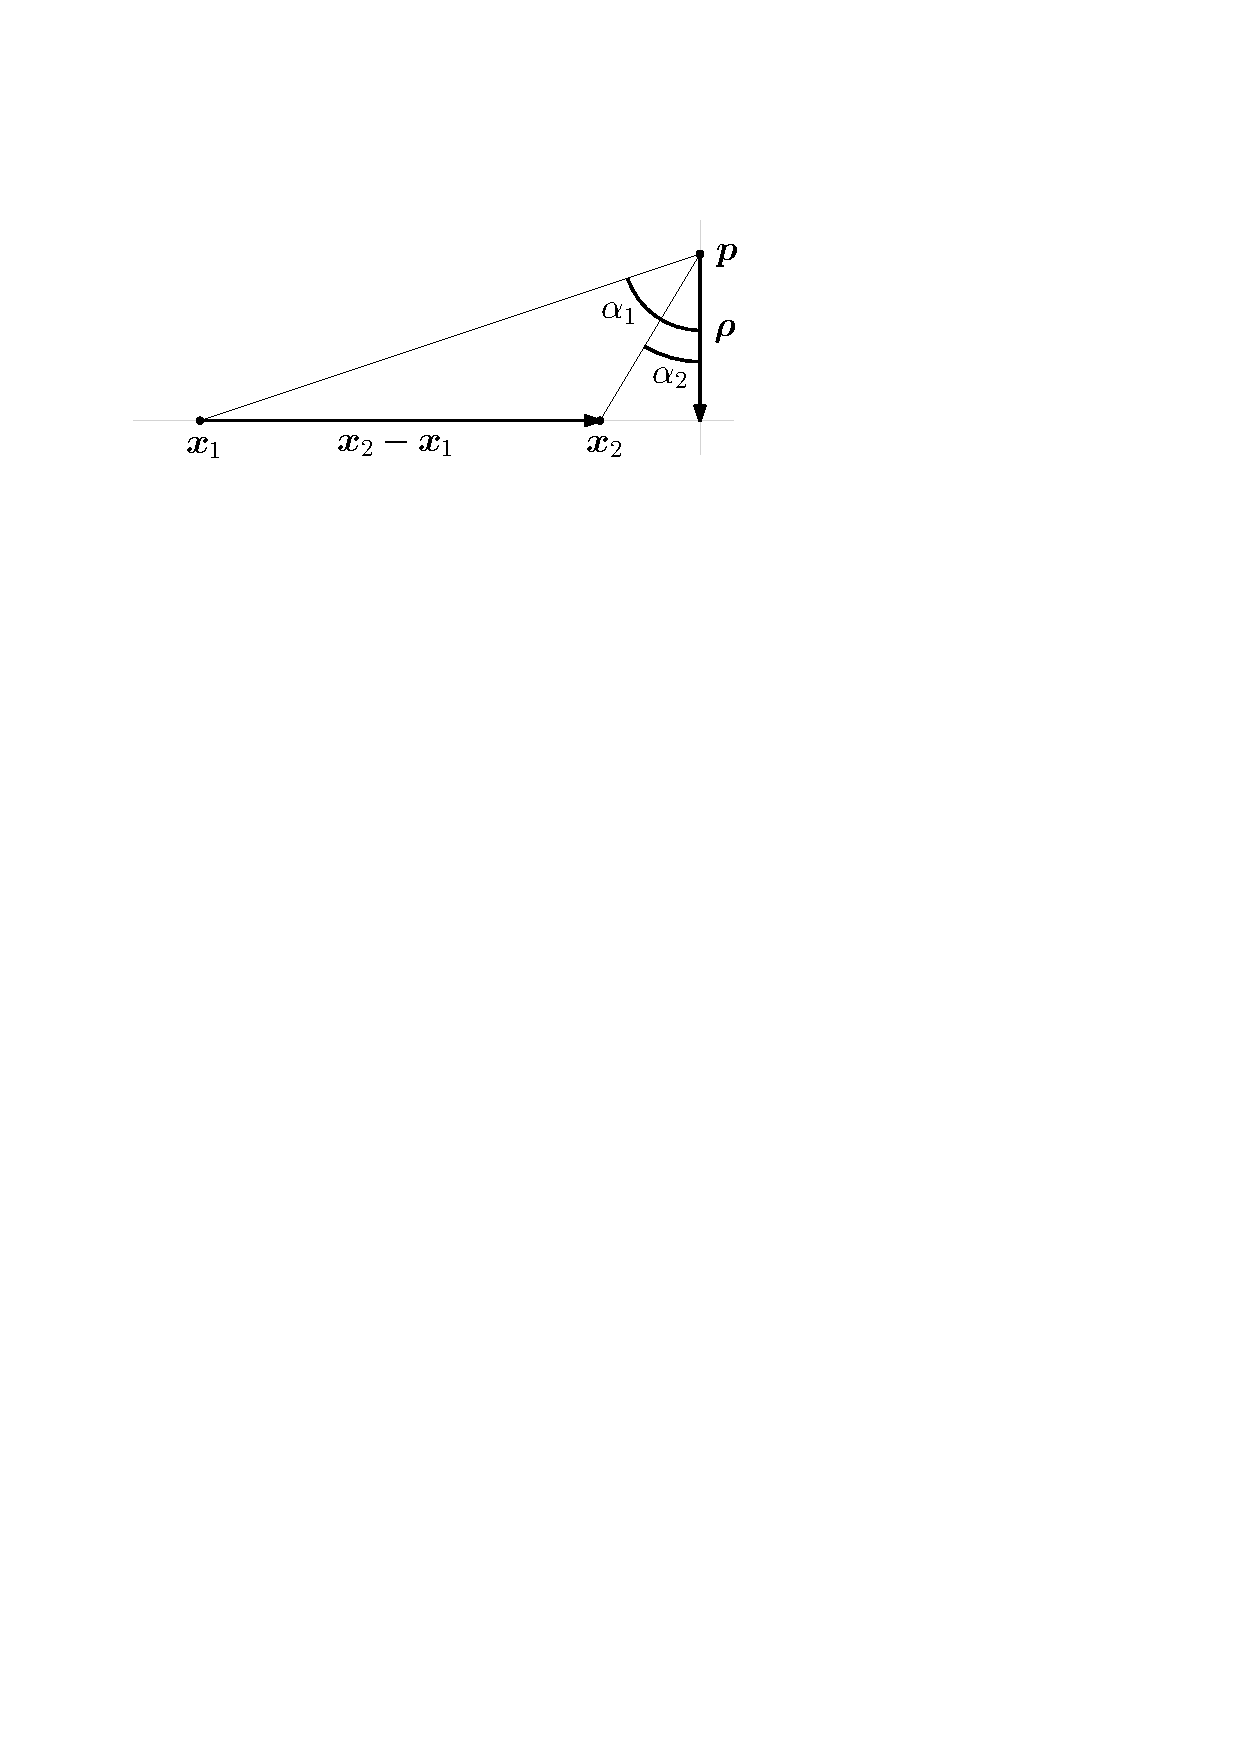
\includegraphics[width=0.6\linewidth]{gfx/coils/biot_savart.pdf}
  \caption{The setting for calculating the magnetic field produced in point $\mathbf{p}$ by a straight wire segment from $\mathbf{x}_1$ to $\mathbf{x}_2$.}\label{fig:biot-savart}
\end{figure}

Imagine four wire segments making up a square loop---a coil. It produces a certain magnetic field in the entire space $\mathbf{B}(\mathbf{x})$, given, following the superposition principle, by a sum of the fields produced by each segment of the coil.
With changing the current in the coil only one parameter of the magnetic field is altered---the magnitude, but not its shape. It can, therefore, be said that one coil spans a one-dimensional space of magnetic fields it can produce. Adding a second, different coil creates a system spanning a two-dimensional space of fields, as the magnetic field is additive. Going a step further, four square coils tiled to form a larger square form a four-dimensional space, as shown in Fig.\,\ref{fig:coils_tile_basis}. Any coil restricted to the $2 \times 2$ grid can be represented in the base of the four tile-coils.

The range of magnetic field reachable by coils restricted to a grid is a subset of all possible fields that can be created with coils constructed on the square's surface. The size of the subset is controlled by $N$, the number of tile-coils forming the grid.
In this system a coil is fully described by a vector of $N$ currents, one in each of the tile-coils, denoted by $\mathbb{I}$. The problem of coil design is thereby simplified to finding a vector $\mathbb{I}$.

\begin{figure}
  \centering
  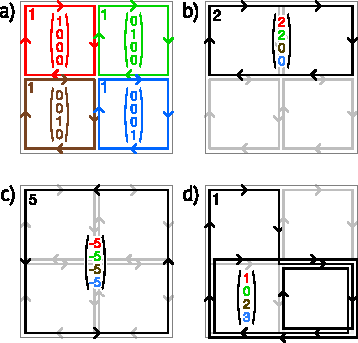
\includegraphics[width=0.6\linewidth]{gfx/coils/tile_basis.pdf}
  \caption{a) A basis of four tile coils on a flat square. Any coil which has its wires restricted to lie on the $2 \times 2$ grid can be represented as a linear combination of the four base tile coils. b, c, d) Three coils are presented together with their explicit coordinates in the basis.}\label{fig:coils_tile_basis}
\end{figure}

Generalisation onto a cube is simple. A cube is made up of six square faces. Interestingly, for the assembly in the three-dimensional space one degree of freedom is lost.  Figure~\ref{fig:coils_tile_kernel} illustrates, in the simplest case $N = 6$, a configuration in which finite currents in all six coils cancel and no magnetic field is produced. Such a combination of currents can be added to any solution with no effect on the produced field. Effectively, the space of the fields they can produce has dimension five (i.e.\ $N-1$). In other words, the mapping of $\mathbb{I}$ onto fields $\mathbf{B}(\mathbf{x})$ has in this case a one-dimensional kernel. This fact is of importance when it comes to numerically solving the system.

\begin{figure}
  \centering
  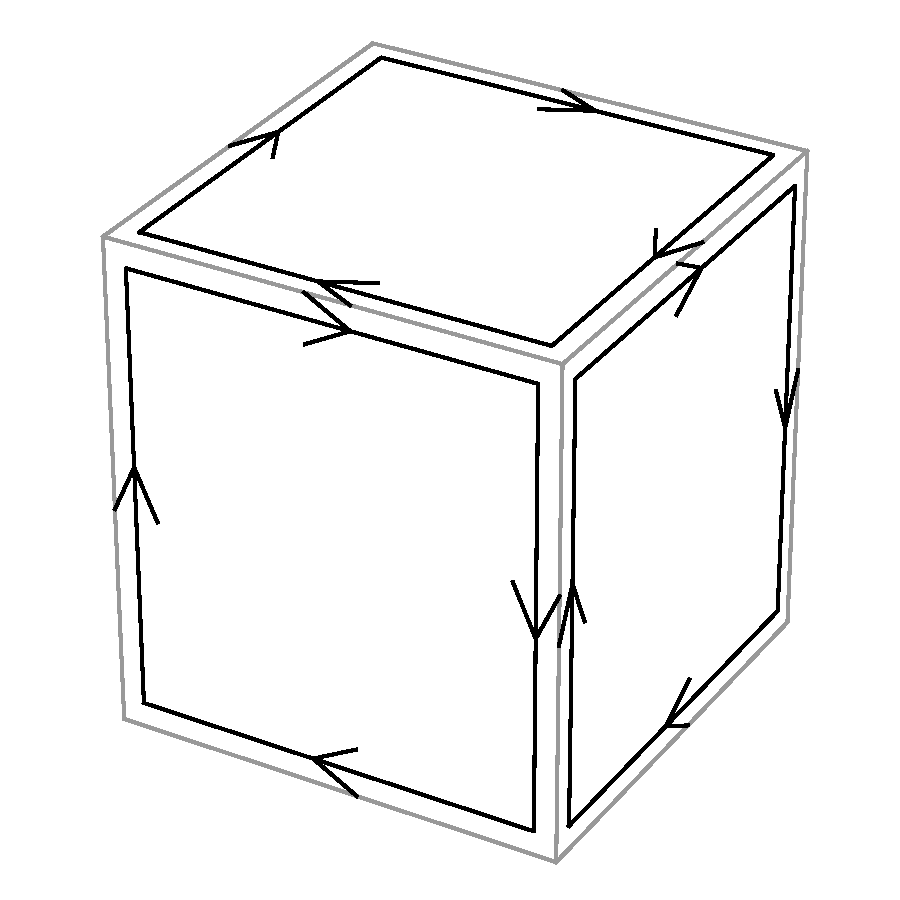
\includegraphics[width=0.5\linewidth]{gfx/coils/tile_kernel2.pdf}
  \caption{An arrangement of $N = 6$ tile coils on a cube which produces no magnetic field. The currents in the tiles are equal and flow in the directions as indicated. The currents on the invisible faces are analogous to the ones seen in front. For clarity, the coils are depicted slightly smaller; in the model the currents are identical with the edges of the cube.}\label{fig:coils_tile_kernel}
\end{figure}

This is the foundation of the method. The restriction to a grid on a cuboid enables all coils in the restricted space to be described by a vector of $N$ numbers.




\section{Coil design}
In the problem of coil design a coil is sought, or an arrangement of coils, which best approximates a given field in a certain volume. The volume we shall call \emph{the volume of interest}. Rather than considering the whole volume, an ensemble of $m$ points of interest on its surface is picked (the surface is sufficient because $\nabla \cdot \mathbf{B} = 0$). Henceforth, the magnetic field $\mathbf{B}(\mathbf{x})$ only at these points is considered. The values $\mathbf{B}(\mathbf{x}_i)$ for $i = 1 .. m$ are gathered into a vector of dimension $3m$ ($B_x$, $B_y$ and $B_z$ in each point), which we shall denote $\mathbb{B}$.

As mentioned before, the magnetic field produced by a coil at any given point in space is proportional to the current in this coil. With many coils present it is a linear combination of the currents of all coils in the system. In an absence of an external magnetic field the system of $N$ tiles and $m$ points of interest is thus described by a simple linear equation:
\begin{equation}
  \label{eq:matrix}
  \mathbb{B} = M \, \mathbb{I}\ ,
\end{equation}
where $M \in \mathbb{R}^{3 m} \times \mathbb{R}^{N}$ is a matrix of proportionality constants. For example, the element $M_{(5, 2)}$ is the proportionality constant between the current in the second of $N$ coils and the magnetic field in the $y$ direction in the second of $m$ points of interest, $B_y(\mathbf{x}_2)$. The matrix $M$ can be calculated analytically using the Biot-Savart law.

Equation~\ref{eq:matrix}, for $3m > N - 1$, is an over-determined system of linear equations, $\mathbb{I}$ being the vector of unknowns. The optimal least-squares solution $\mathbb{I}_0$ to produce a $\mathbf{B}_0(\mathbf{x})$ in the volume of interest is
\begin{equation}
  \label{eq:requirement}
  % M \, \mathbb{I} \stackrel{!}{=} \mathbb{B}_0
  \mathbb{I}_0 = \arg\,\min_{\mathbb{I}} {\left( M \mathbb{I} - \mathbb{B}_0 \right)}^2 \ .
\end{equation}
The optimal solution can be calculated with the normal equation~\cite{Anton}:
\begin{equation}
  \mathbb{I}_0 = {\left( M^\mathrm{T} M \right)}^{-1} M^\mathrm{T} \mathbb{B}_0 \ ,
\end{equation}
\marginpar{Least-squares is solved with a backslash operator in MATLAB-like languages:\\
\texttt{I0 = M \textbackslash{} B0.}}
but the problem is typically solved numerically. The majority of numerical software packages use the QR decomposition (a product of an orthogonal and upper-triangular matrix) of the matrix $M$, which is more numerically stable when compared to the normal equation.

Depending on the properties of $M$ the optimum may be multidimensional. In particular, as already mentioned, an arrangement of coils on a cube has a one-dimensional kernel, which will always cause the optimum to be at least one-dimensional. In these cases, we will call $\mathbb{I}_0$ the unique least-norm solution, which minimizes the total current in the system. $\mathbb{I}_0$ is the vector of the optimal currents in the tile arrangement of coils for approximating $\mathbf{B}_0(\mathbf{x})$ in the volume of interest.

\begin{figure}
  \centering
  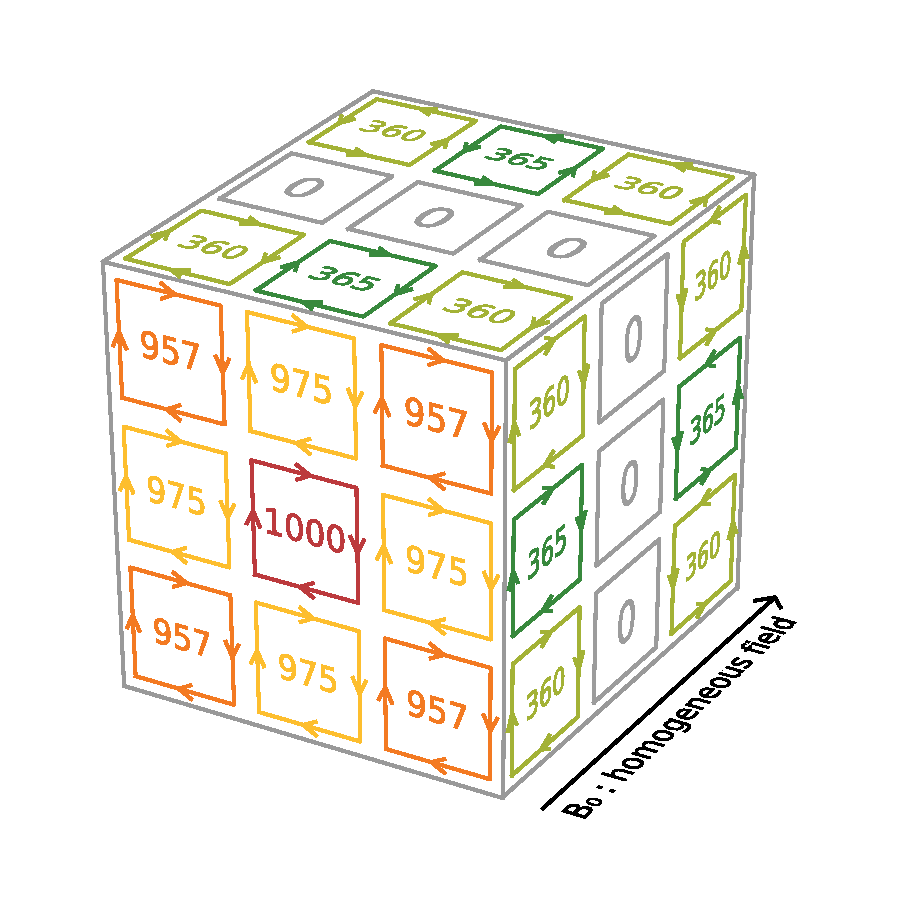
\includegraphics[width=\linewidth]{gfx/coils/homogeneous_tiles_norm_1000.pdf}
  \caption{A solution of a tile system with $N = 6 \times (3 \times 3)$ tiles on a unit cube for a homogeneous field. The volume of interest is a cube with side length \num{0.75}, centered inside the unit cube. Numbers indicate currents in the tile coils in arbitrary units. The currents are normalized so that the highest is \num{1000}. For clarity, the coils are depicted slightly smaller; in the model their edges overlap. The currents on the three invisible faces are by symmetry analogous to the visible ones.}\label{fig:homogeneous_tiles}
\end{figure}

\begin{figure*}
  \centering
  \subfloat{\label{fig:homogeneous_performance_a}
    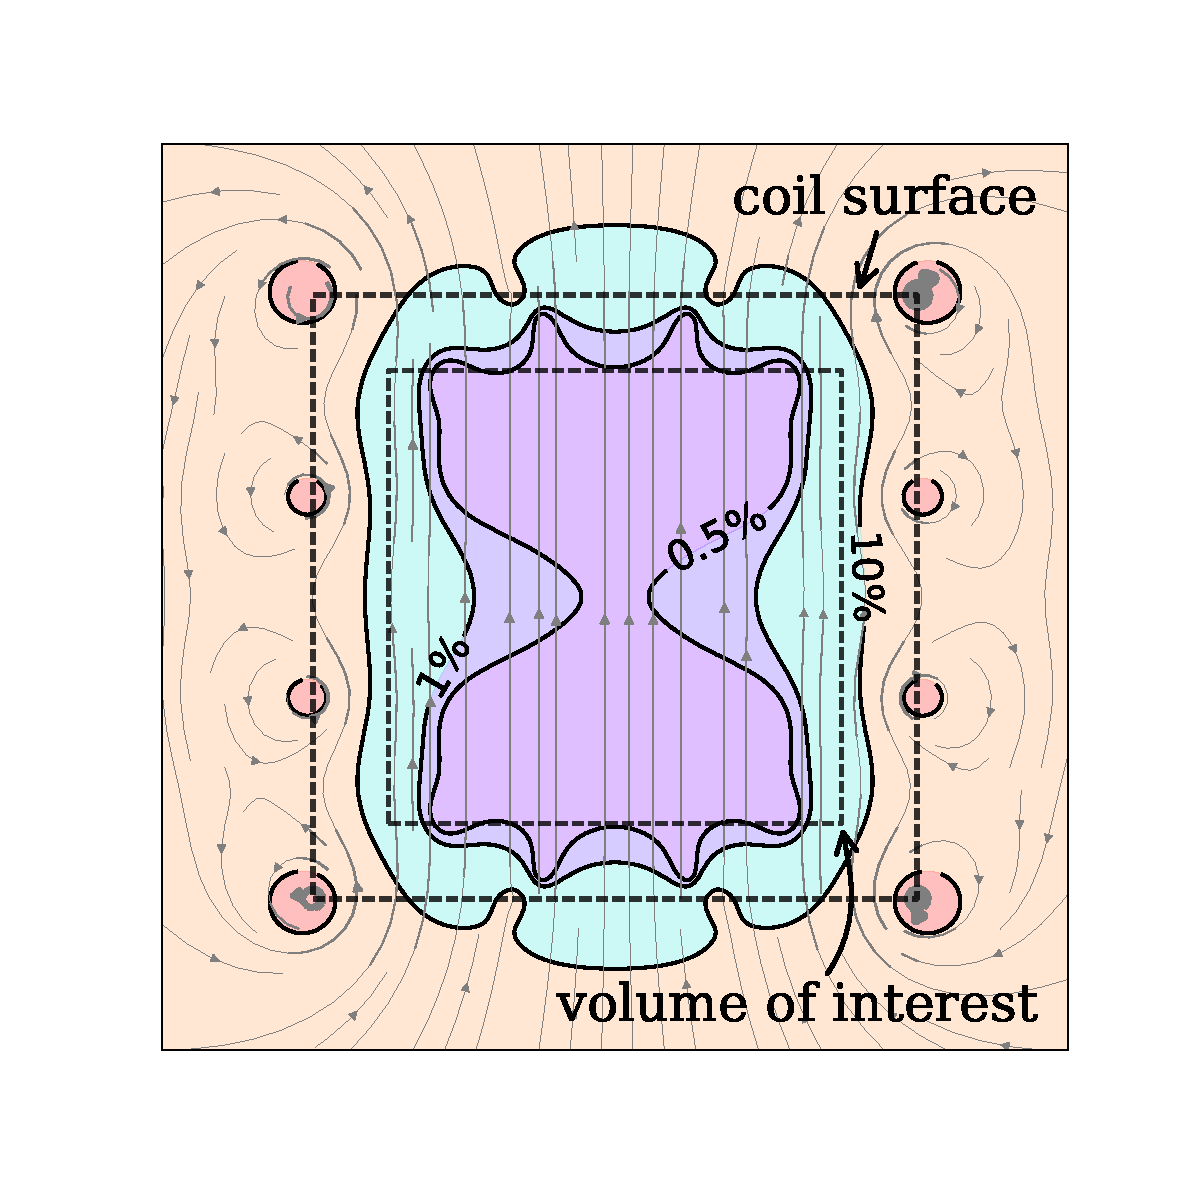
\includegraphics[width=.49\linewidth]{gfx/coils/homogeneous_performance.pdf}}
  \subfloat{\label{fig:homogeneous_performance_b}
    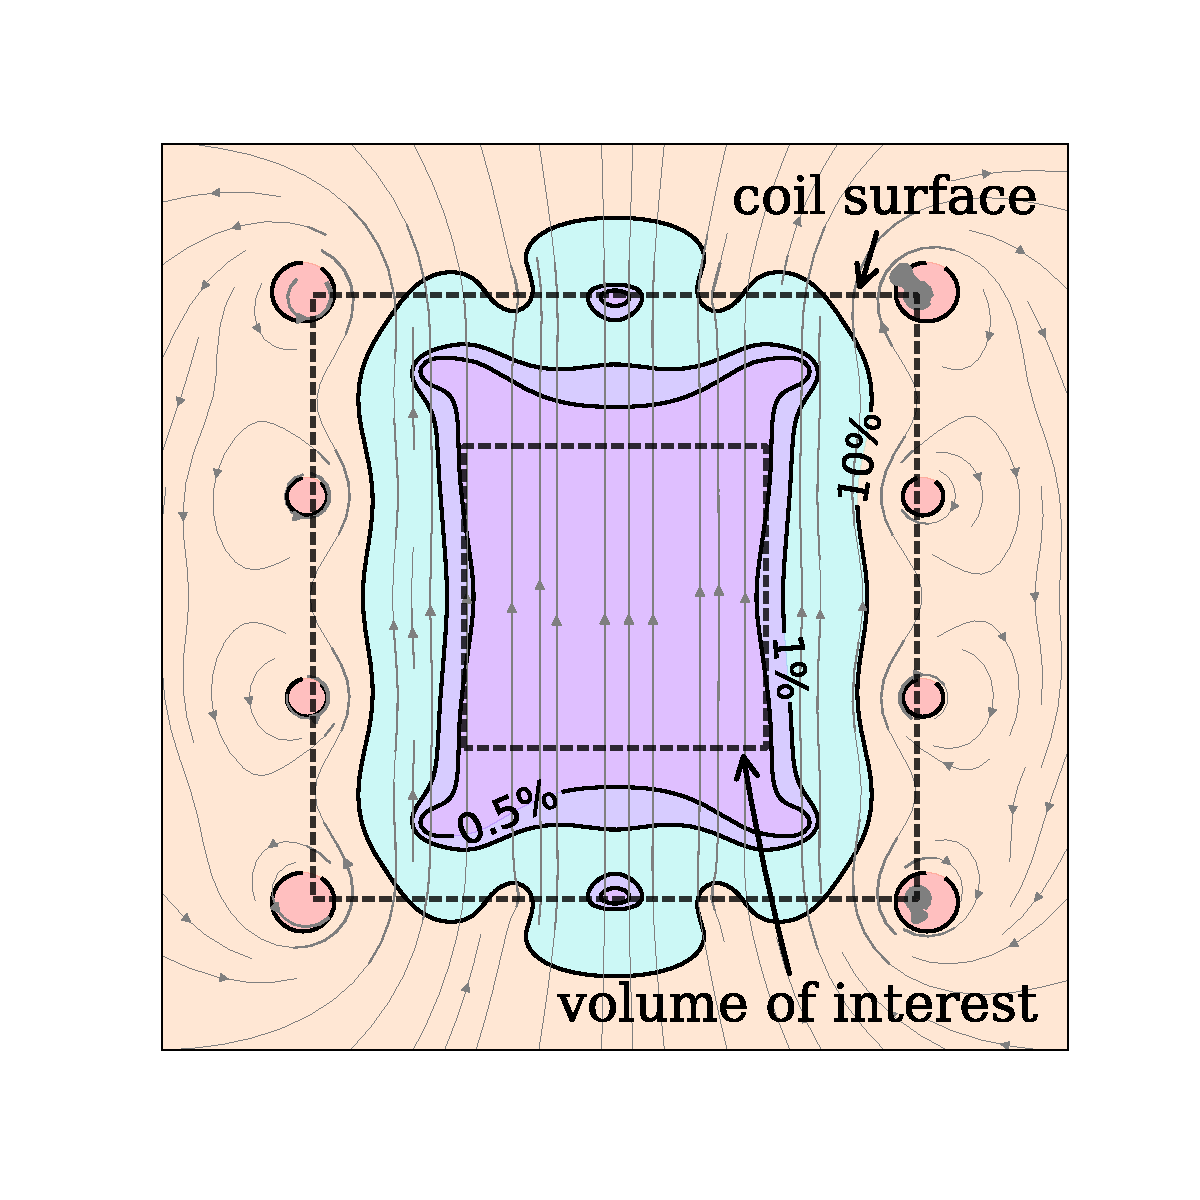
\includegraphics[width=.49\linewidth]{gfx/coils/homogeneous_performance_smaller_volume.pdf}}
  \caption{Magnetic field produced by a coil designed for a homogeneous field, with $N = 6 \times (3 \times 3)$ tiles on a unit cube. The field lines are depicted in grey. Contours show boundaries of \num{0.5}, \num{1} and \SI{10}{\percent} magnitude deviation from an ideal homogeneous field. Horizontal cross sections in the middle-height plane are shown. Two designs are presented. Left-hand side: the volume of interest is a cube with side length \num{0.75} (the individual tile coil currents are depicted in Fig.\,\ref{fig:homogeneous_tiles}), right-hand side: the size of volume of interest is reduced to \num{0.5}.}\label{fig:homogeneous_performance}
\end{figure*}

Let us consider an example of a coil design on a unit cube with the number of tiles $N = 6 \times (3 \times 3)$ (see Fig.\,\ref{fig:homogeneous_tiles}). As the volume of interest we pick a cube, centered with the unit one, with side length \num{0.75} (with a regular mesh of $10 \times 10$ points on each face, a total of $m = 488$ points of interest). For the sake of simplicity we design a coil for a homogeneous field along an axis of the cube. The solution of Eq.\,\ref{eq:requirement}, $\mathbb{I}_0$, directly gives the currents in each tile. They are graphically depicted in Fig.\,\ref{fig:homogeneous_tiles}. Note, that many currents almost cancel each other, in particular those along horizontal edges. The magnetic field produced by the solution is shown on the left-hand side in Fig.\,\ref{fig:homogeneous_performance}, as a horizontal cut along the central plane. Contours show the relative deviation from the homogeneous field. Inside the volume of interest (dashed line), the design goal of a homogeneous field is reproduced with few per cent accuracy. The solution, and thus the contours too, depend on the choice of the volume of interest. In general, the further away the volume of interest is from the coils, the better the accuracy. If the side length of the volume of interest is decreased to \num{0.5}, the accuracy improves to \SI{1}{\percent}, as shown on the right-hand side in Fig.\,\ref{fig:homogeneous_performance}. The optimal solution, and thereby the shape of the precision contours, change. Naturally, the accuracy of the field reproduction can also be improved by increasing the number of tiles.




\section{Simplification of the tile system}
The tile system may find an interesting practical application. Once independently controllable tiles have been built, it can be used to produce an arbitrary field. However, building many independently driven coils is a high price to pay for producing only one field. Additionally, each edge is shared between two tiles, and the effective current is the sum of two. They may add either constructively or destructively. If the given solution is dominated by subtraction of large currents, a lot of power is unnecessarily dissipated in the system. It turns out, that both problems can be solved by simplifying the tile solution.

\begin{figure*}
  \centering
  \subfloat{\label{fig:coils_dipole_3d_1}
    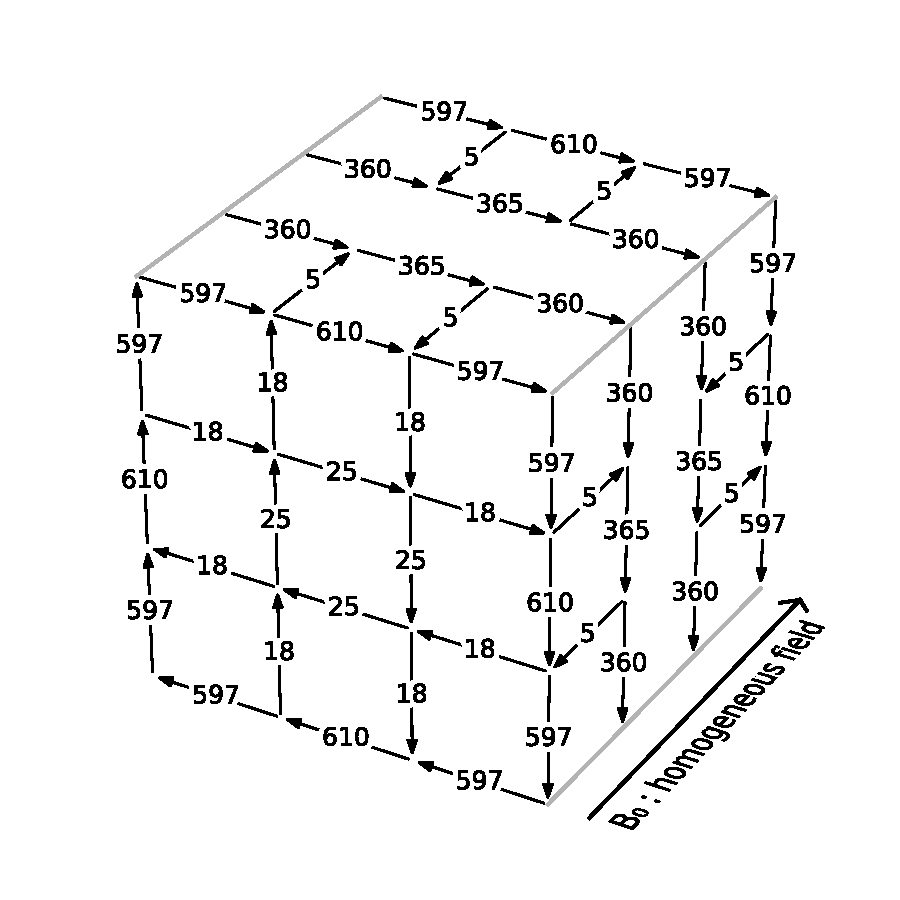
\includegraphics[width=.49\linewidth]{gfx/coils/algorithm_net_1.pdf}}
  \subfloat{\label{fig:coils_dipole_section_0}
    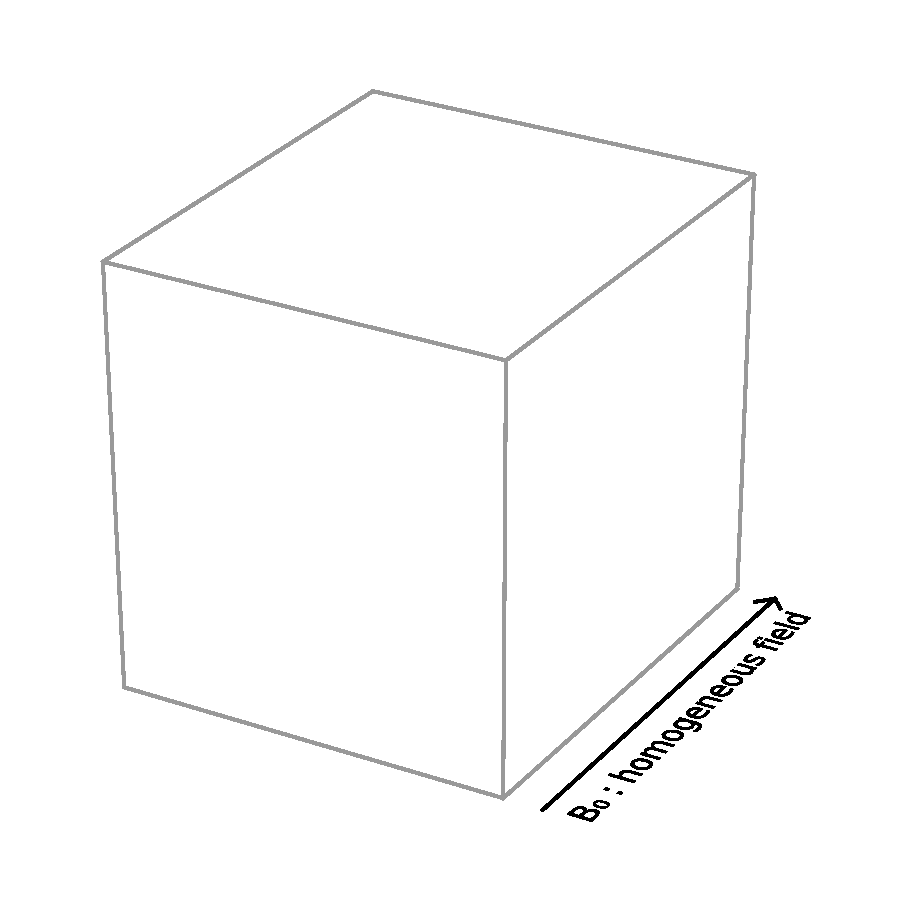
\includegraphics[width=.49\linewidth]{gfx/coils/algorithm_simplified_0.pdf}}
  \\
  \subfloat{\label{fig:coils_dipole_3d_3}
    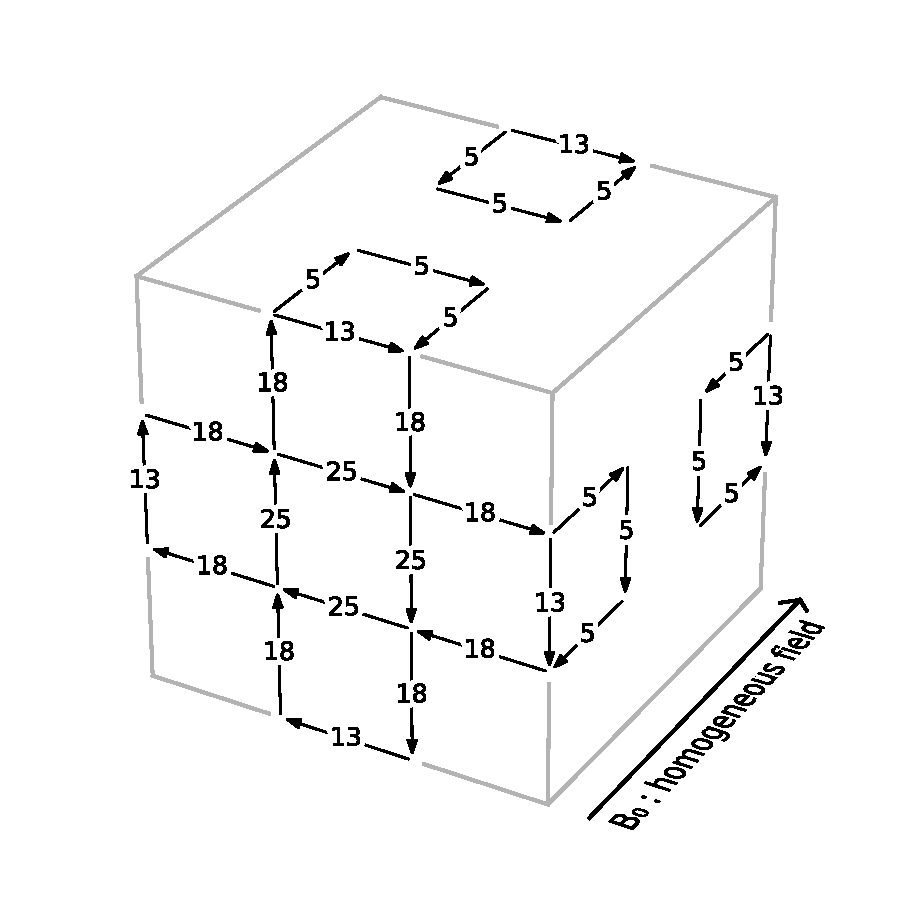
\includegraphics[width=.49\linewidth]{gfx/coils/algorithm_net_3.pdf}}
  \subfloat{\label{fig:coils_dipole_section_2}
    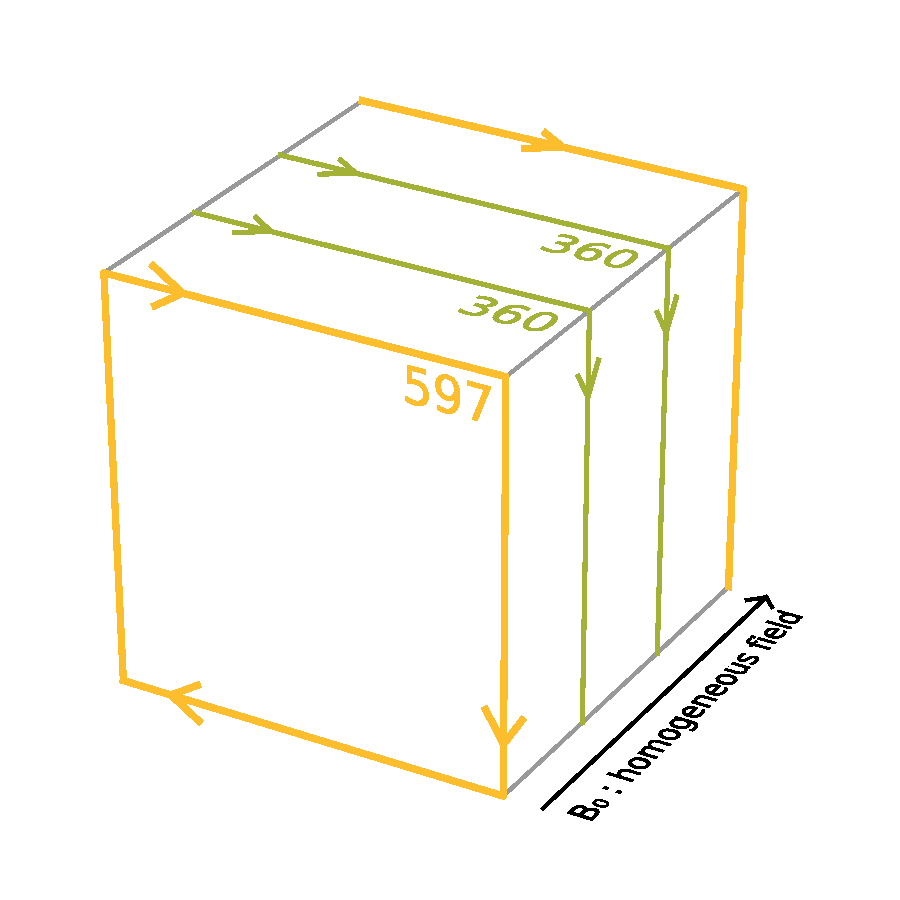
\includegraphics[width=.49\linewidth]{gfx/coils/algorithm_simplified_2.pdf}}
  \\
  \subfloat{\label{fig:coils_dipole_3d_5}
    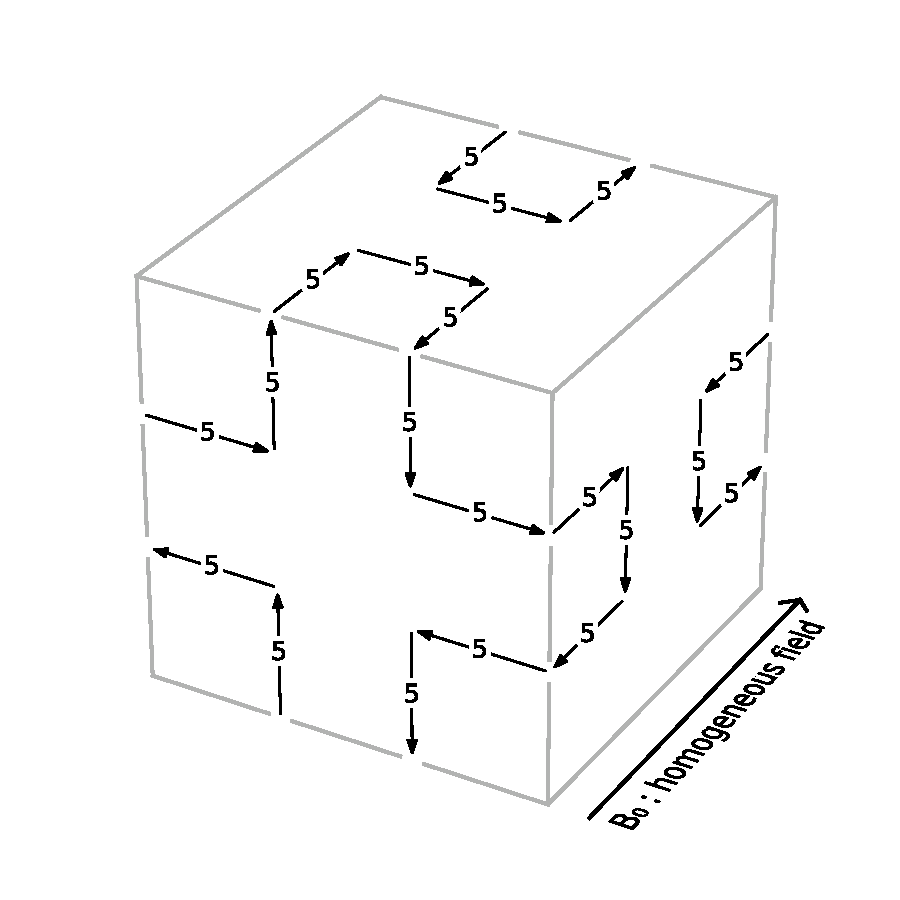
\includegraphics[width=.49\linewidth]{gfx/coils/algorithm_net_5.pdf}}
  \subfloat{\label{fig:coils_dipole_section_4}
    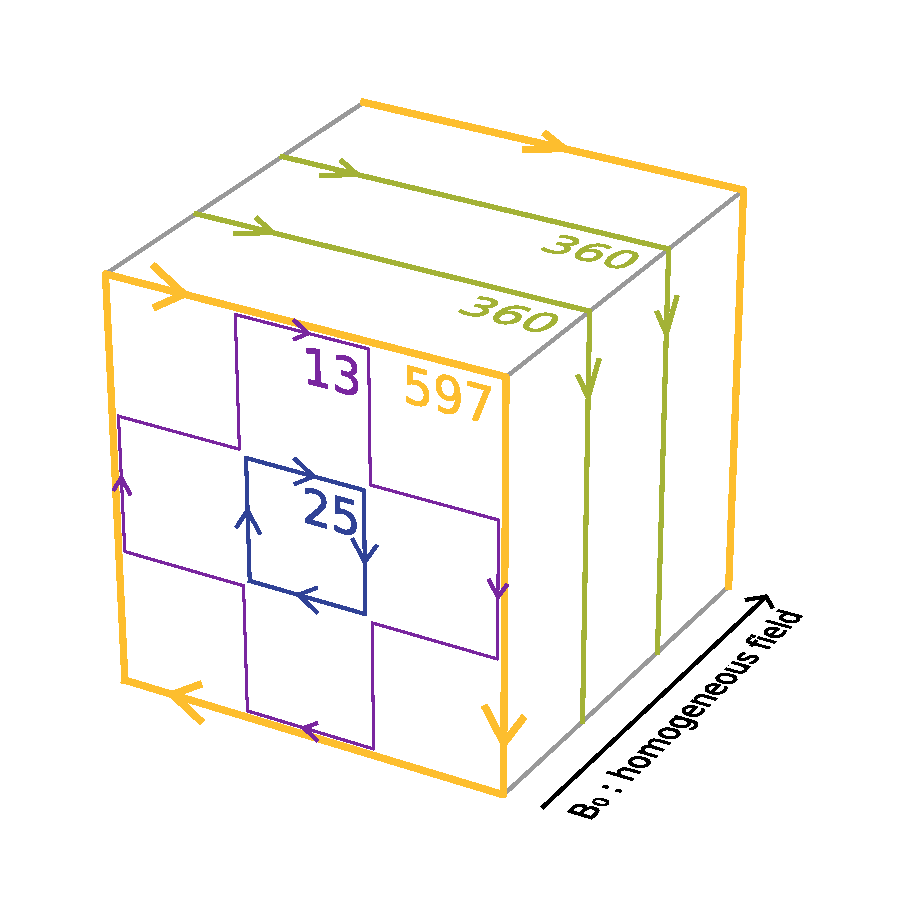
\includegraphics[width=.49\linewidth]{gfx/coils/algorithm_simplified_4.pdf}}
  \caption{Following the algorithm to simplify a coil. The left column shows the net of a current with the total current along edges of tiles. In each iteration the loop with the highest current is found and transferred onto the simplified solution, shown in the right column. We show iterations, from top: zeroth, fourth and eighth.}\label{fig:simplification_algorithm}
\end{figure*}

\begin{figure}
  \centering
  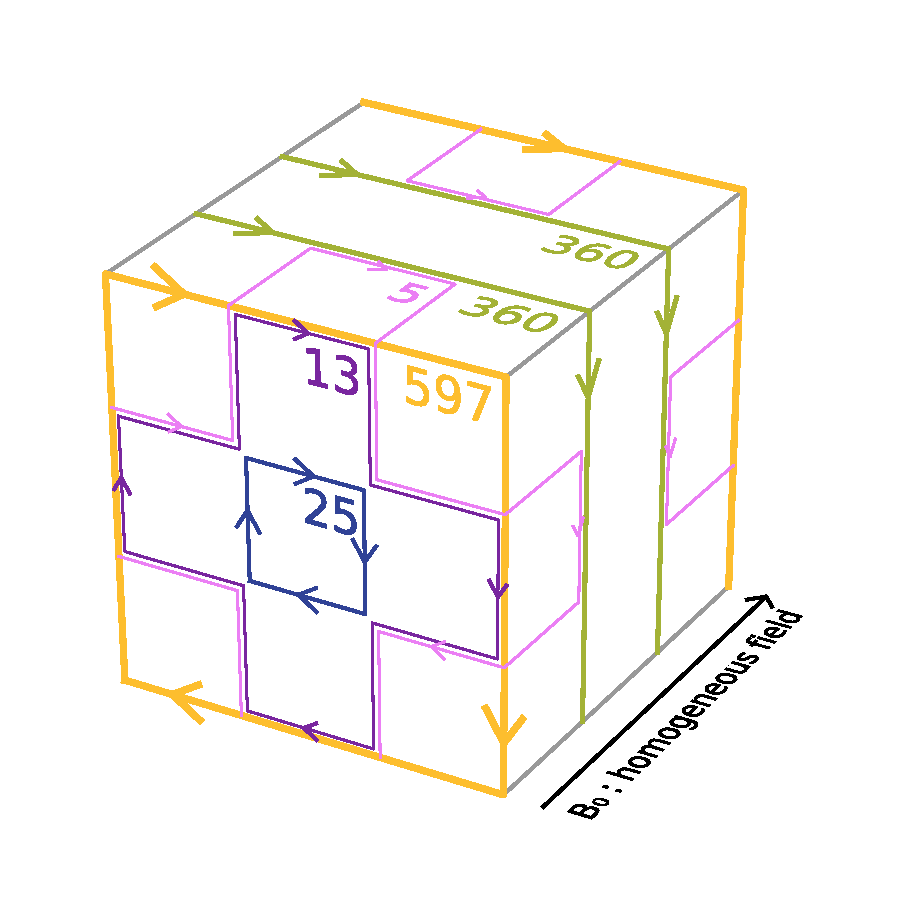
\includegraphics[width=\linewidth]{gfx/coils/algorithm_simplified_5.pdf}
  \caption{The coil designed for a homogeneous field, with $N = 6 \times (3 \times 3)$ tiles (Fig.\,\ref{fig:homogeneous_tiles}), simplified by adding the currents along each edge and decomposing into current loops.}\label{fig:homogeneous_coils}
\end{figure}

One starts by adding the currents of the adjacent tiles and assigning the sum to each common edge. The result is a complicated net of currents (upper left corner of Fig.\,\ref{fig:simplification_algorithm}). Still, each node fulfills Kirchhoff's laws. The net can then be decomposed into simple current loops by following the algorithm: First find in the net the loop with the highest current. In the example it is either of the ``\num{597}'' loops on the front and back faces. This loop will make the first one in the simplified solution (it can be seen in the middle of the right column in Fig.\,\ref{fig:simplification_algorithm}, together with the next three loops). Then subtract from the net the current of the first loop along its edges (the net that remains after subtracting the first four loops is depicted in the middle of the left column in Fig.\,\ref{fig:simplification_algorithm}). Finally, continue to find the loop with the highest current in the modified net, which will give the next loop and repeat until the current net is empty. The net remaining after eight loops are found is depicted in the bottom row of Fig.\,\ref{fig:simplification_algorithm}, next to the first eight loops. The final simplified solution is shown in Fig.\,\ref{fig:homogeneous_coils}. The currents in the simplified coil system are much smaller, the highest being \num{597} instead of \num{1000} and they always add constructively. Also, the number of separate loops is decreased from \num{42} to \num{10}. Still, the total current along each edge of a tile is exactly the same as in the tile configuration.

We conclude here our method of coil design. The simplified arrangement of coils is the optimal one, given the grid restriction, for approximating the magnetic field in the volume of interest. We continue to consider practical aspects, relevant for constructing the designs of the new method.




\section{Practical considerations}
The primary practical advantage of the new design method is that the coils are constrained to a predefined grid. This is contrary to other methods of coil design, where the position of the wires is the output of the procedure~\cite{Turner1993, Beidler1990}. This may prove useful in applications with spatial constraints. Typically, coils need to be incorporated into a setup in which other components penetrate the surface on which the wires are laid. In the new method it is possible to simply define the grid so that no collisions occur. Although the simple examples presented before used regular grids, we have not used symmetries to solve the problem. When many coils are designed and built, for instance to produce homogeneous magnetic fields in each of the three dimensions, they can all share the same grid. The grid can, for example, be constructed out of cable channels into which the wires are laid.

A limitation associated with the finite size of the channels is the strength of the magnetic field that can be created, which, for given available power, is limited by the thickness of the wire. At the same time, the finite size of the cable channels can be neglected in the calculations only as long as it is small compared to the distance between the coils and the volume of interest. Using an enameled wire, rather than a standard, PVC-insulated cable, can reduce the overall thickness.

In the proposed solution in order to produce the desired field one still needs a system of several coils, even in the simplified solution. The more complicated the goal field, and the more tiles, the more different currents are needed across the individual loops, which quickly becomes impractical. There are several ways to tackle the problem.

The first way is to use only one current and adjust by varying the number of windings. In the example, when one decides for \num{60} windings as the maximum, then the nominal current that would flow through the wire is $\mathrm{round}(597 / 60) = 10$. The \num{597}, \num{360}, \num{25}, \num{13} and \num{5} would be created with \num{60}, \num{36}, \num{3}, \num{1} and \num{1} windings, respectively. A discretisation error of $10 / 597 = \SI{1.7}{\percent}$ is of the same order as the accuracy of the solution in representing the field (see Fig.\,\ref{fig:homogeneous_performance}). For more precise designs the numbers of windings get larger, which is troublesome to construct and causes the coils to have larger inductances.

A second way is to use a current divider. That is to connect the different loops in parallel, each with an appropriately chosen resistance in series. This way the ratios between the currents in each loop can be tuned precisely. However, a practical realization will most likely involve routing all loops out of the system where the current divider is installed. For more complicated coil systems with tens of different currents this may be impractical.

Yet another way is to split the loops into decades of currents.
In the coil we use as an example, the currents \num{597}, \num{360}, \num{13}, \num{7}, \num{5} (in arbitrary units) may be constructed from a set of wires with three relative currents of \num{100}, \num{10} and \num{1}:
\marginpar{A base different than 10 can be used, too.}
\begin{align*}
  597 & = 5 \times 100 + 9 \times 10 + 7 \times 1 \\
  360 & = 3 \times 100 + 6 \times 10 + 0 \times 1 \\
  13 & = 0 \times 100 + 1 \times 10 + 3 \times 1 \\
  7 & = 0 \times 100 + 0 \times 10 + 7 \times 1 \\
  5 & = 0 \times 100 + 0 \times 10 + 5 \times 1 \ .
\end{align*}
In this way accuracy better than \SI{1}{\percent} in reproducing the solution can be reached with only three different currents to control, even for complicated designs. Those can be either separately controlled or split with a current divider.

No claim is made as to superiority of one of the three above solutions over the other two. It is up to the particular application which is the best suited one.




\section{Application to active magnetic field shielding}
Using the method presented here to design coils of an active magnetic shield  offers improvements in two areas. Firstly, the size of the coils could be decreased, or the size of the experimental set-up increased, without loss of performance. Better homogeneity in a given volume can always be achieved by choosing a denser gird. Given the tight spatial constraints this was a crucial development for the design of the n2EDM's active shield.

\begin{table}
  \centering
  \begin{tabular}{c|ccc}
    n & $\mathbf{P}_n^x(\mathbf{r})$ & $P_n^y(\mathbf{r})$ & $P_n^y(\mathbf{r})$ \\ \midrule
    1 & 1 & 0 & 0 \\
    2 & 0 & 1 & 0 \\
    3 & 0 & 0 & 1 \\
    \midrule
    4 & $x$ &  0  & $-z$ \\
    5 & $y$ & $x$ &   0  \\
    6 &  0  & $y$ & $-z$ \\
    7 & $z$ &  0  & $ x$ \\
    8 &  0  & $z$ & $-y$ \\
  \end{tabular}
  \caption{Cartesian harmonic polynomials.}\label{tab:coils_cartesian_harmonics}
\end{table}

Secondly, the method allows to construct a coil for any field. In particular, one may choose to construct coils that produce fields orthogonal to one another. 
% (as $\mathbb{R}^3 \rightarrow \mathbb{R}^3$ functions).
This makes an active shielding system significantly easier to control~\cite{MRM:MRM1910010107} and avoids a potential problem of the high condition number due to very-high-order fields produced by pathological combinations of coils (recall the discussion in Sec.\,\ref{sec:nedm_sfc_matrix}). One of the possible orthogonal decompositions of the field is the one into \emph{cartesian harmonic polynomials}~\cite{Franke2013}:
\begin{equation}
  \mathbf{B}(\mathbf{r}) = \sum_{n}\,H_n \mathbf{P}_n(\mathbf{r}) \ ,
\end{equation}
where $H_n$ are the expansion coefficients, and $\mathbf{P}_n(\mathbf{r})$ are the cartesian harmonic polynomials, the first eight of which are listed in Table~\ref{tab:coils_cartesian_harmonics}. Each term satisfies by itself the Maxwell's equations. The first three terms are homogeneous fields, the next five are the five independent linear gradients. Further ones correspond to higher-order gradients.

\begin{figure*}
  \centering
  \subfloat{\label{fig:coils_dipole_3d}
    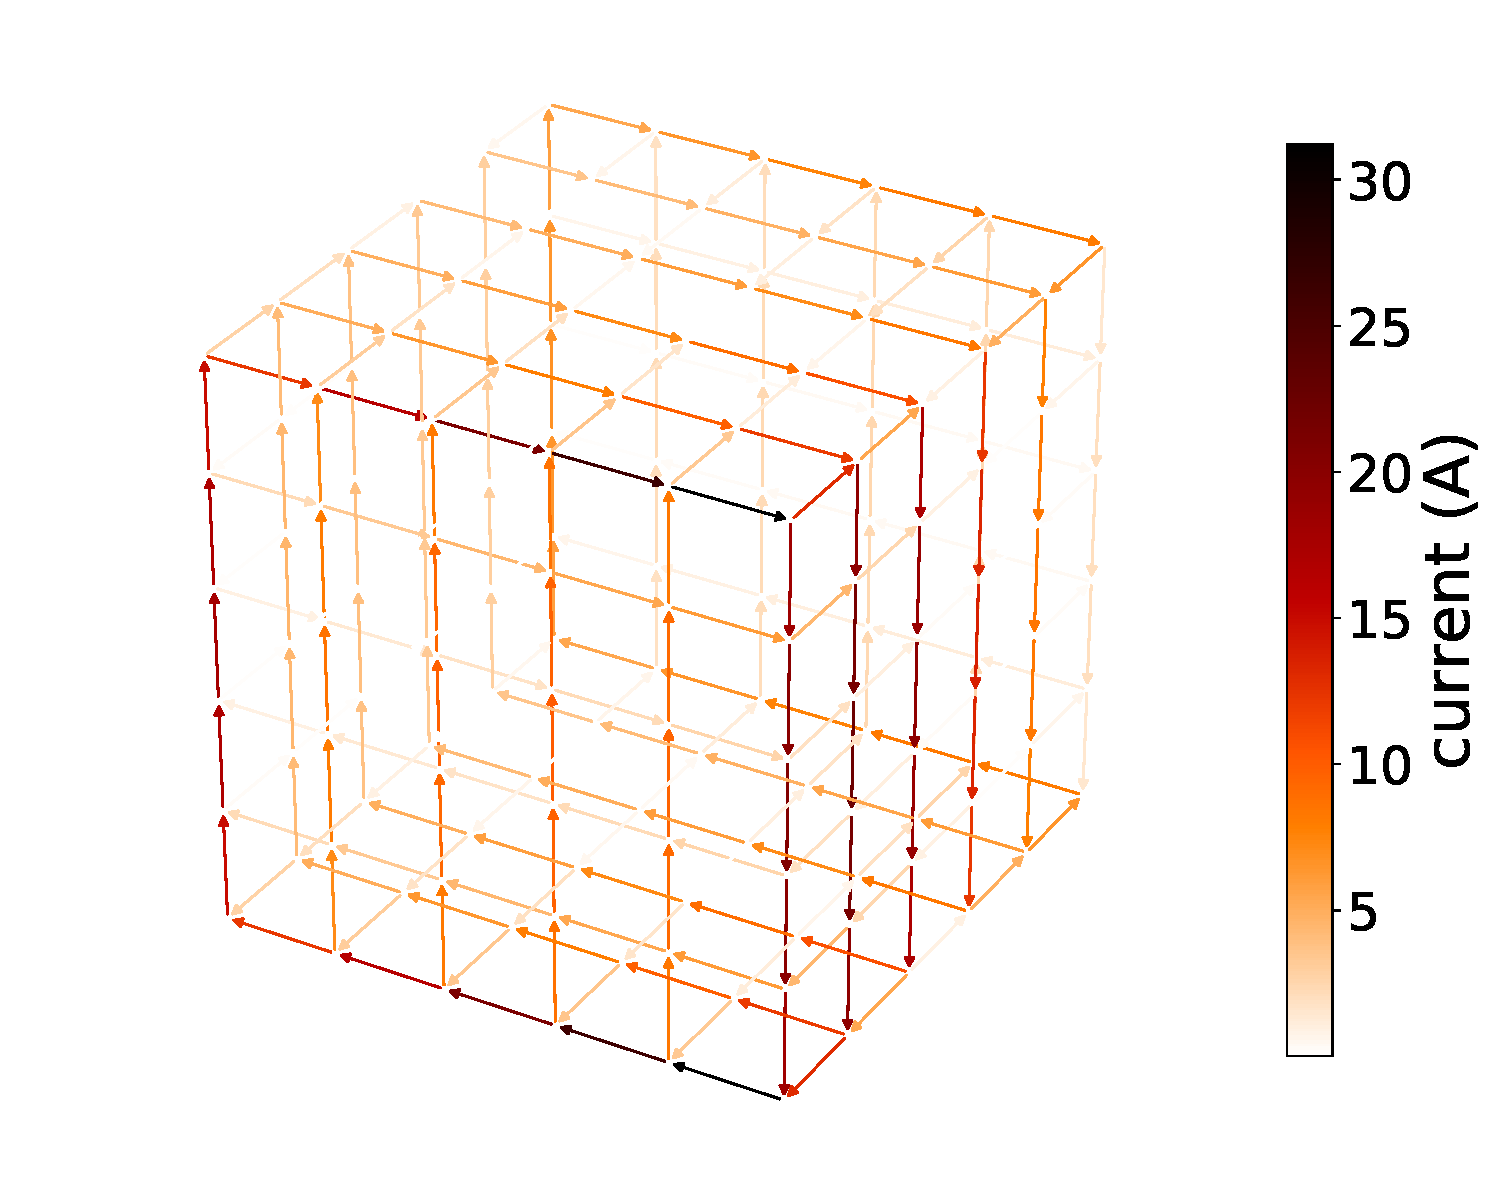
\includegraphics[width=.39\linewidth]{gfx/coils/coil_dipole.pdf}}
  \subfloat{\label{fig:coils_dipole_section}
    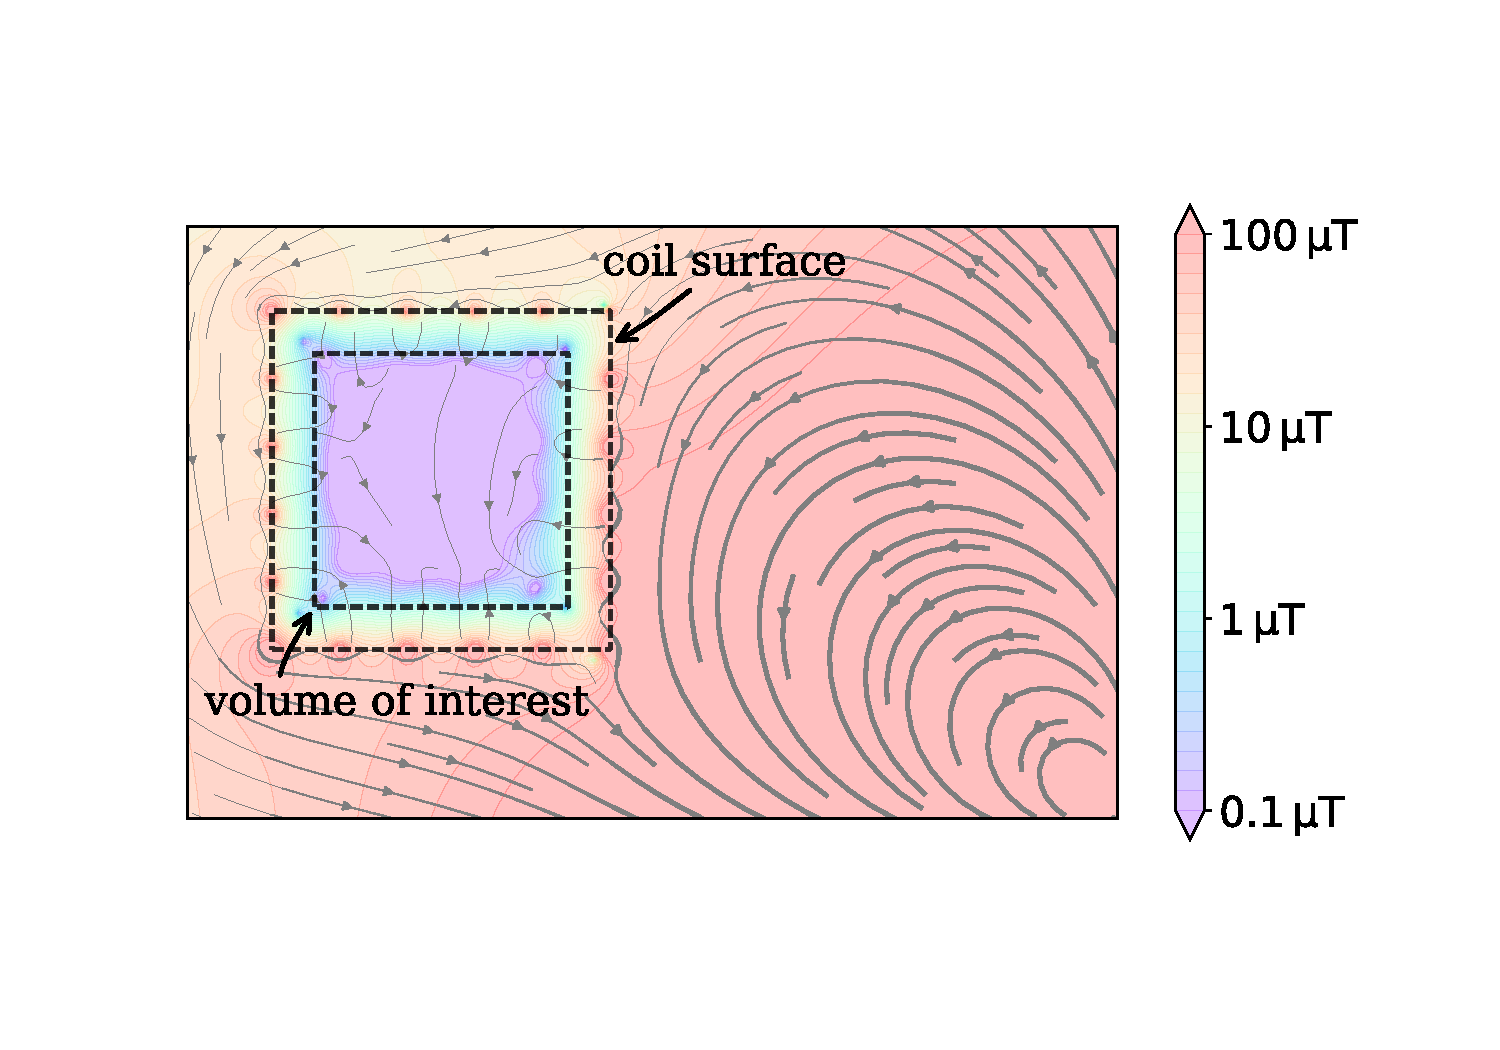
\includegraphics[width=.59\linewidth]{gfx/coils/coil_dipole_section_with_dipole.pdf}}
  \caption{A coil designed on a unit cube with $5 \times 5$ tiles per face to shield against a dipole disturbance. The dipole is located, relative to the center of the unit cube, two units to the right and one unit to the front. It is located in the middle height of the cube. The volume of interest has a side length of \num{0.75}. On the left-hand side the total current along each edge of the dipole compensation coil is depicted. On the right-hand side the magnetic field is shown. The magnetic field lines are shown in grey, the volume of interest and the coil surface with dashed lines. The colors depict the magnitude of the magnetic field (capped at \num{0.1} and \SI{100}{\micro\tesla}). A horizontal cross section in the middle height is shown. The dipole source is located in the lower right corner of the plot and points parallel to the plane of the plot. The magnitude of the field in the volume of interest is reduced from tens of microteslas down to below one.}\label{fig:showcase}
\end{figure*}

Additionally, one can consider constructing dedicated coils to counteract a particular known disturbance. In Fig.\,\ref{fig:showcase}, a showcase design with $N = 6 \times (5 \times 5) = 150$ tiles for compensating a nearby dipole source is presented.

Last, but not least, the method's unique property of designing on a predefined grid makes a large-scale construction particularly feasible. It makes it easy to be incorporated into the existing structures, by defining the grid in a conflict-free way.




\section*{Coil design -- conclusion}
Coil design is a complicated and very technical problem, especially when high accuracy is required. This work presents a method that is simple in terms of both underlying math and computational effort. The design method could find its niche in practical applications, where spatial constraints play a significant role and a percent level in accuracy of the produced field is acceptable. The method has particular advantages when used to design coils of an active magnetic field compensation system. In the next chapter, its application to construction of a compensation system at the ETH Zürich is described.

The software implementation of the coil design, including examples, has been published as open-source~\cite{Coilsjlcode}.

% !TEX root = ../rawlik-phd-thesis.tex
\chapter{Next generation active magnetic field compensation}
\label{ch:sfc-prototype}

The coil design method described in the previous chapter opened the door to a next generation of active magnetic field compensation systems. Ones where the coil system is not much larger than the fiducial volume and where high-order terms of the magnetic field can be compensated, all while retaining a low number of controlled degrees of freedom.

% The large fiducial volume is of particular importance for the n2EDM experiment at PSI. The available area\ldots

In the laboratory at ETH Zürich an active magnetic field compensation system was constructed, based on the coil design. The goal was do demonstrate the feasibility of construction of the coils, develop and test the electronic and software parts of the feedback algorithm, and test system as the whole.

\note{Schwammig, work on it!}


\section{The first iteration --- coil structure}
In the discussion of the coil design method a possible way to realise it in practice was indicated---to construct a grid out of cable channels. The system, pictured in Fig.\,\ref{fig:prototype_photo}, was built as $5 \times 9 \times 5$ grid of square tiles. Each tile had side length \SI{262}{\milli\meter}, the total size was $1310 \times 1310 \times \SI{2358}{\milli\meter}$. The vertical axis we refer to as $z$, the long horizontal one as $y$, and the remaining as $x$. The support frame was made of aluminum construction profiles. To support the cable channels, on each side there was a large, one-piece aluminum sheet with square cut-outs leaving the material only directly below the cable channels. The plastic cable channels were glued onto the aluminum.

\begin{sidewaysfigure}
  \centering
  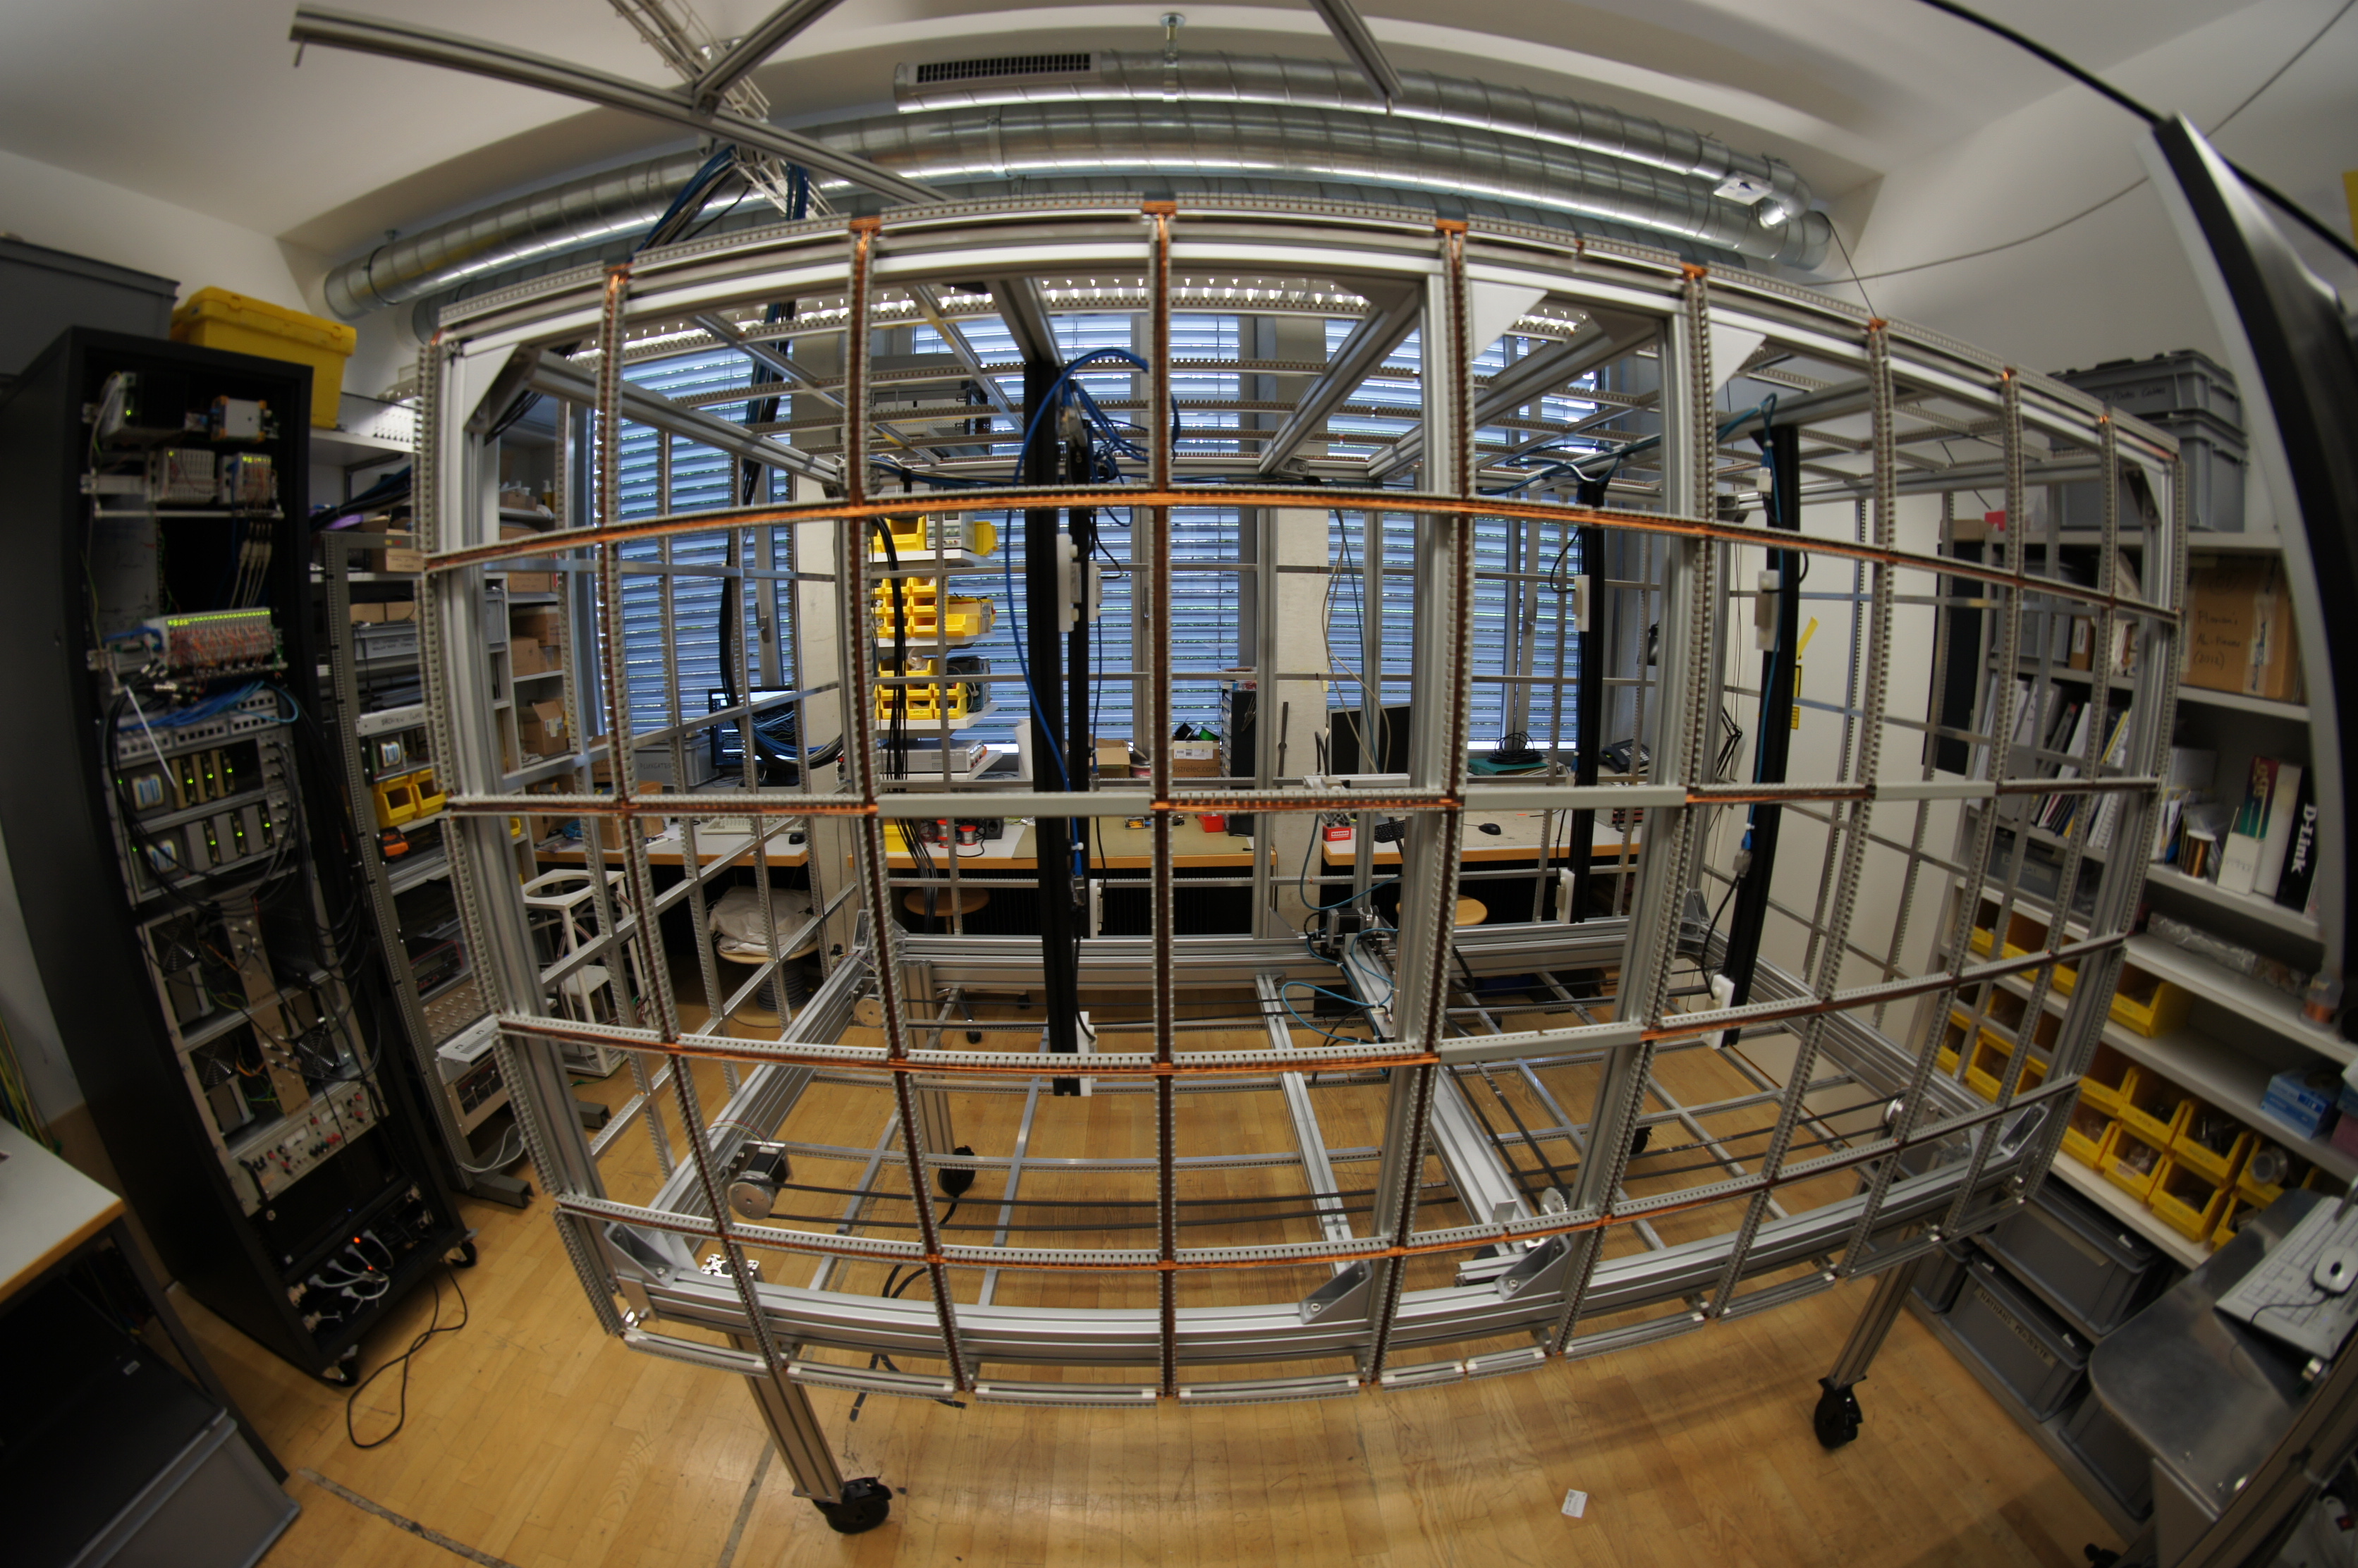
\includegraphics[width=0.75\linewidth]{gfx/prototype/DSC03472.JPG}
  \caption{The active magnetic compensation system in the laboratory at ETH Zürich. It consists cable channels mounted on an aluminum support structure. In the channels copper wires making up the coils can be seen. On the left-hand side the control cabinet of the system is visible.}\label{fig:prototype_photo}
\end{sidewaysfigure}

\begin{figure}
  \centering
  % 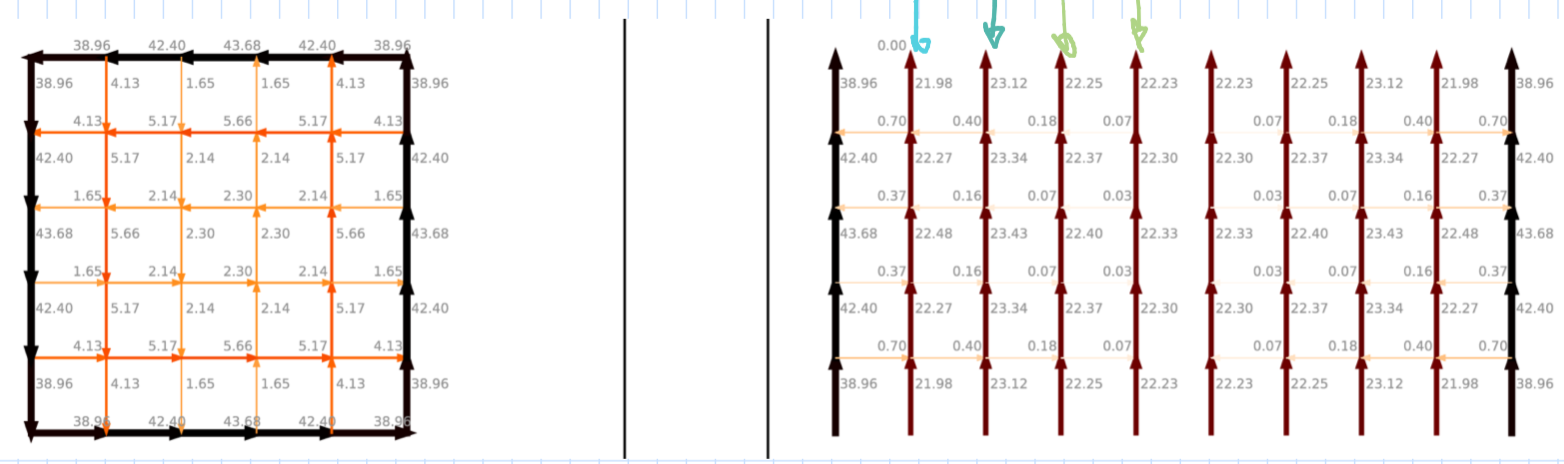
\includegraphics[width=0.9\linewidth]{gfx/prototype/coil_y_currents.png}
  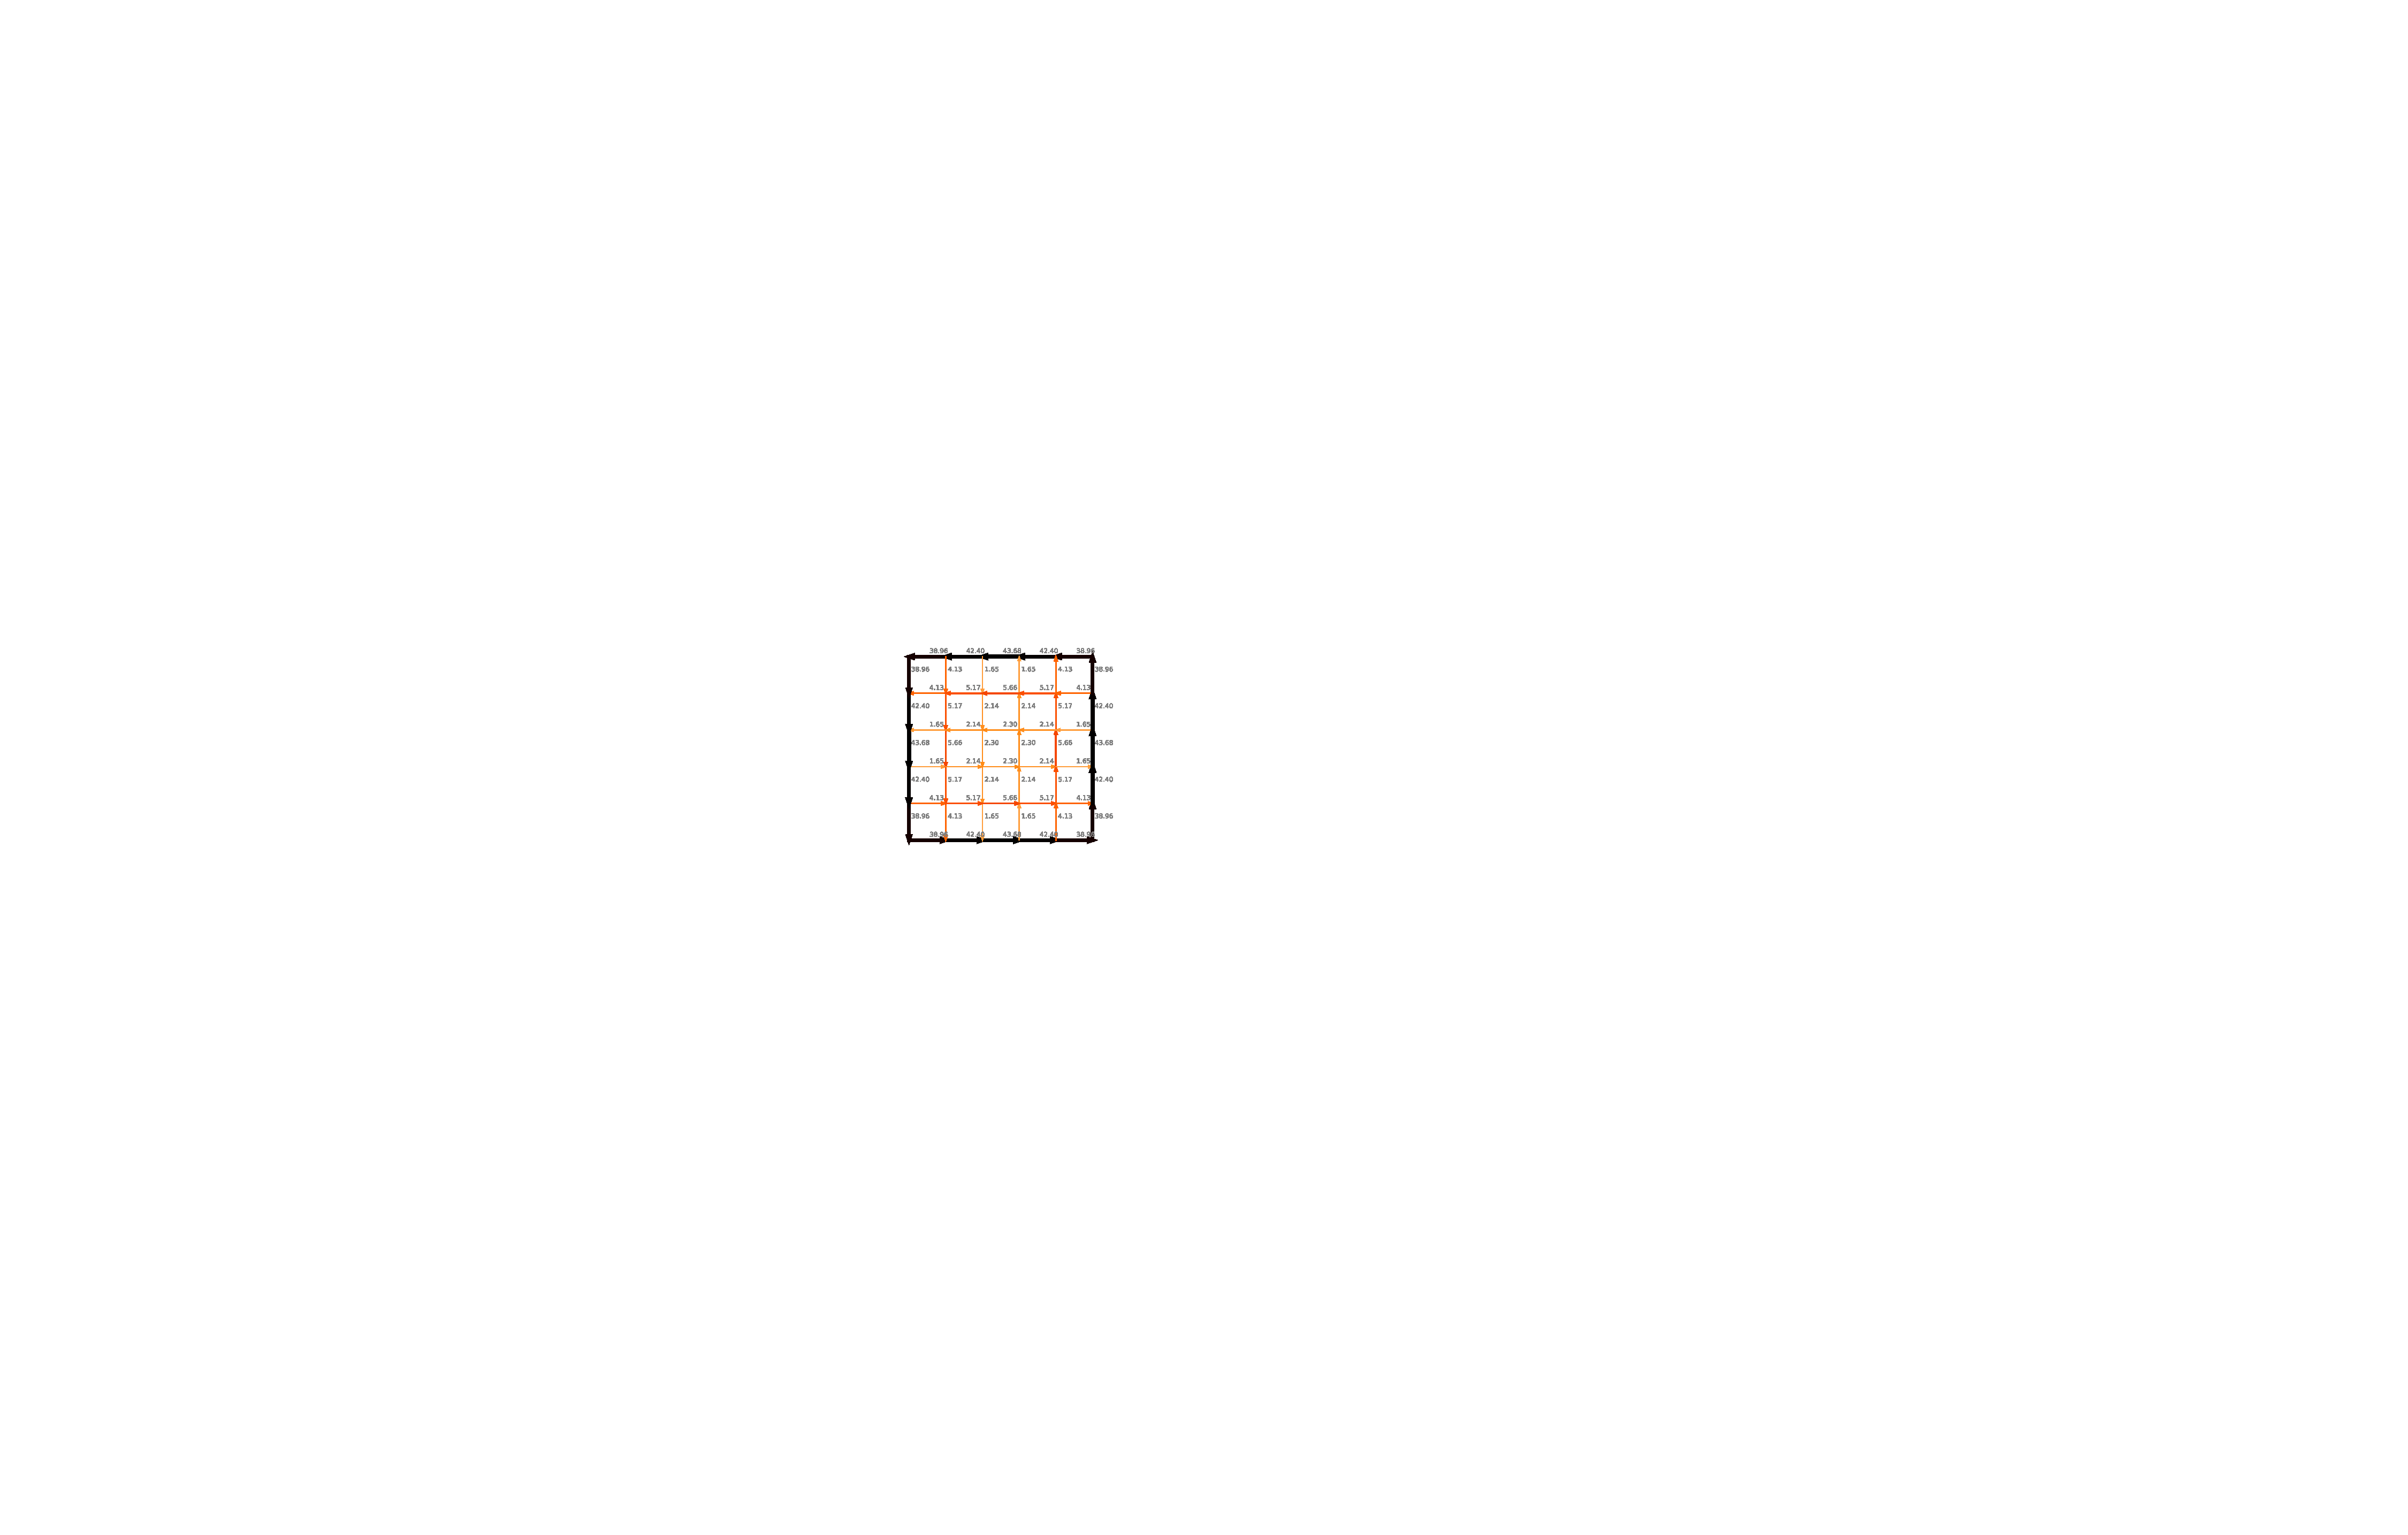
\includegraphics[height=0.3\linewidth]{gfx/prototype/coil_design_y_100uT_1.pdf}
  \quad\quad
  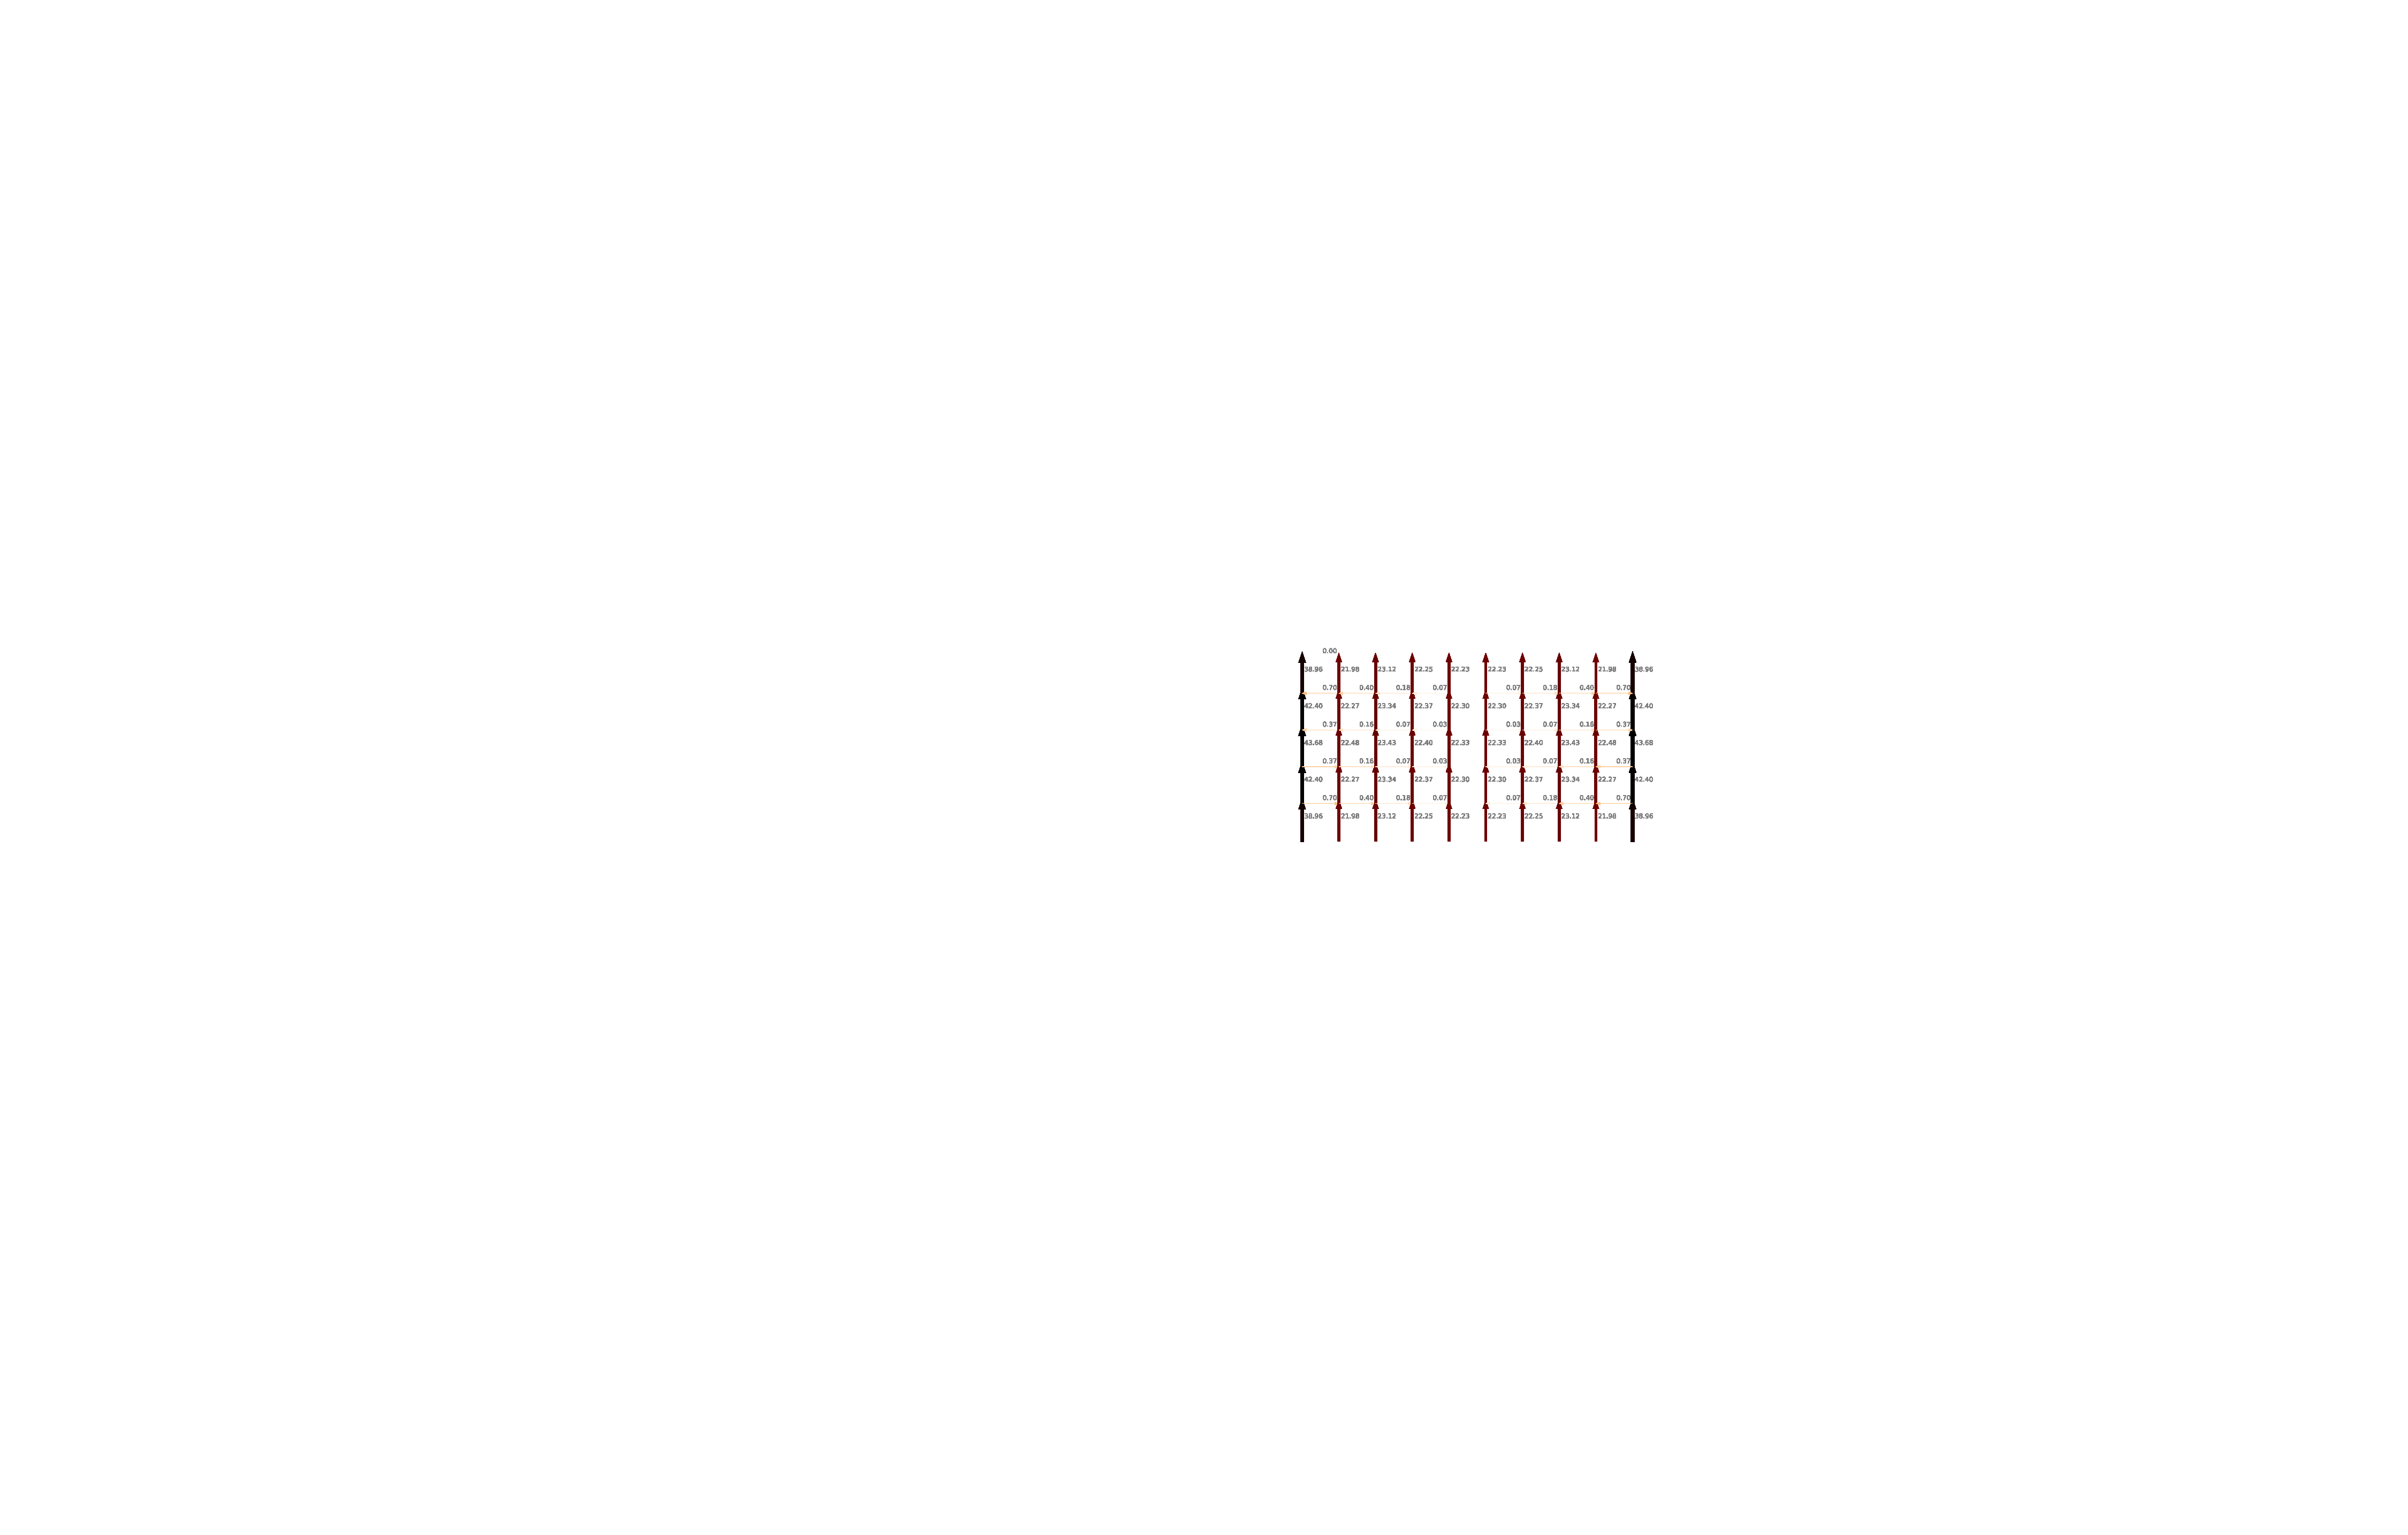
\includegraphics[height=0.3\linewidth]{gfx/prototype/coil_design_y_100uT_2.pdf}
  \caption{The optimal current net for the $y$-coil of the ETH active magnetic field compensation system. Both $5 \times 5$ faces ($y = \mathrm{const}$ planes) are identical and are depicted on the left-hand side. The rectangular faces are all identical, and are depicted on the right-hand side. For each segment the current per \SI{100}{\micro\tesla} of generated field is indicated upwards and to the right from its centre.}\label{fig:prototype_coil_y_currents}
\end{figure}

In its first version the system featured three coils for the homogeneous components of the magnetic field (the first three cartesian harmonics). The coils were designed following the method described in the previous chapter, but excluding the, not ready at the time, simplification algorithm. The simplification was carried out manually instead. The fiducial volume was chosen to be a cuboid centred in the system, with each of its face \SI{155}{\milli\meter} away from the surface of the coils. The optimal current net for the $y$-coil (producing a homogeneous field in the $y$ direction) is depicted in Fig.\,\ref{fig:prototype_coil_y_currents} and its manual decomposition into loops in Fig.\,\ref{fig:prototype_coil_y_decomposition}. The design promised a 2\% homogeneity inside the fiducial volume. The current net for $x$- and $z$-coils, identical to each other on symmetry grounds, is depicted in Fig.\,\ref{fig:prototype_coil_x_z_currents}.
Finally, the individual loops were discretised into \SI{10}{\ampere}, \SI{2}{\ampere} and \SI{0.2}{\ampere}, per nominal \SI{100}{\micro\tesla}. For example, the \SI{38.96}{\ampere} current, indicated in black in Fig.\,\ref{fig:prototype_coil_y_decomposition}, was realised as three windings of the \SI{10}{\ampere} wire, four of the \SI{2}{\ampere} one and five of the \SI{0.2}{\ampere} one.
% and the decomposition in Fig.\,\ref{fig:prototype_coil_x_z_decomposition}.

\begin{figure}
  \centering
  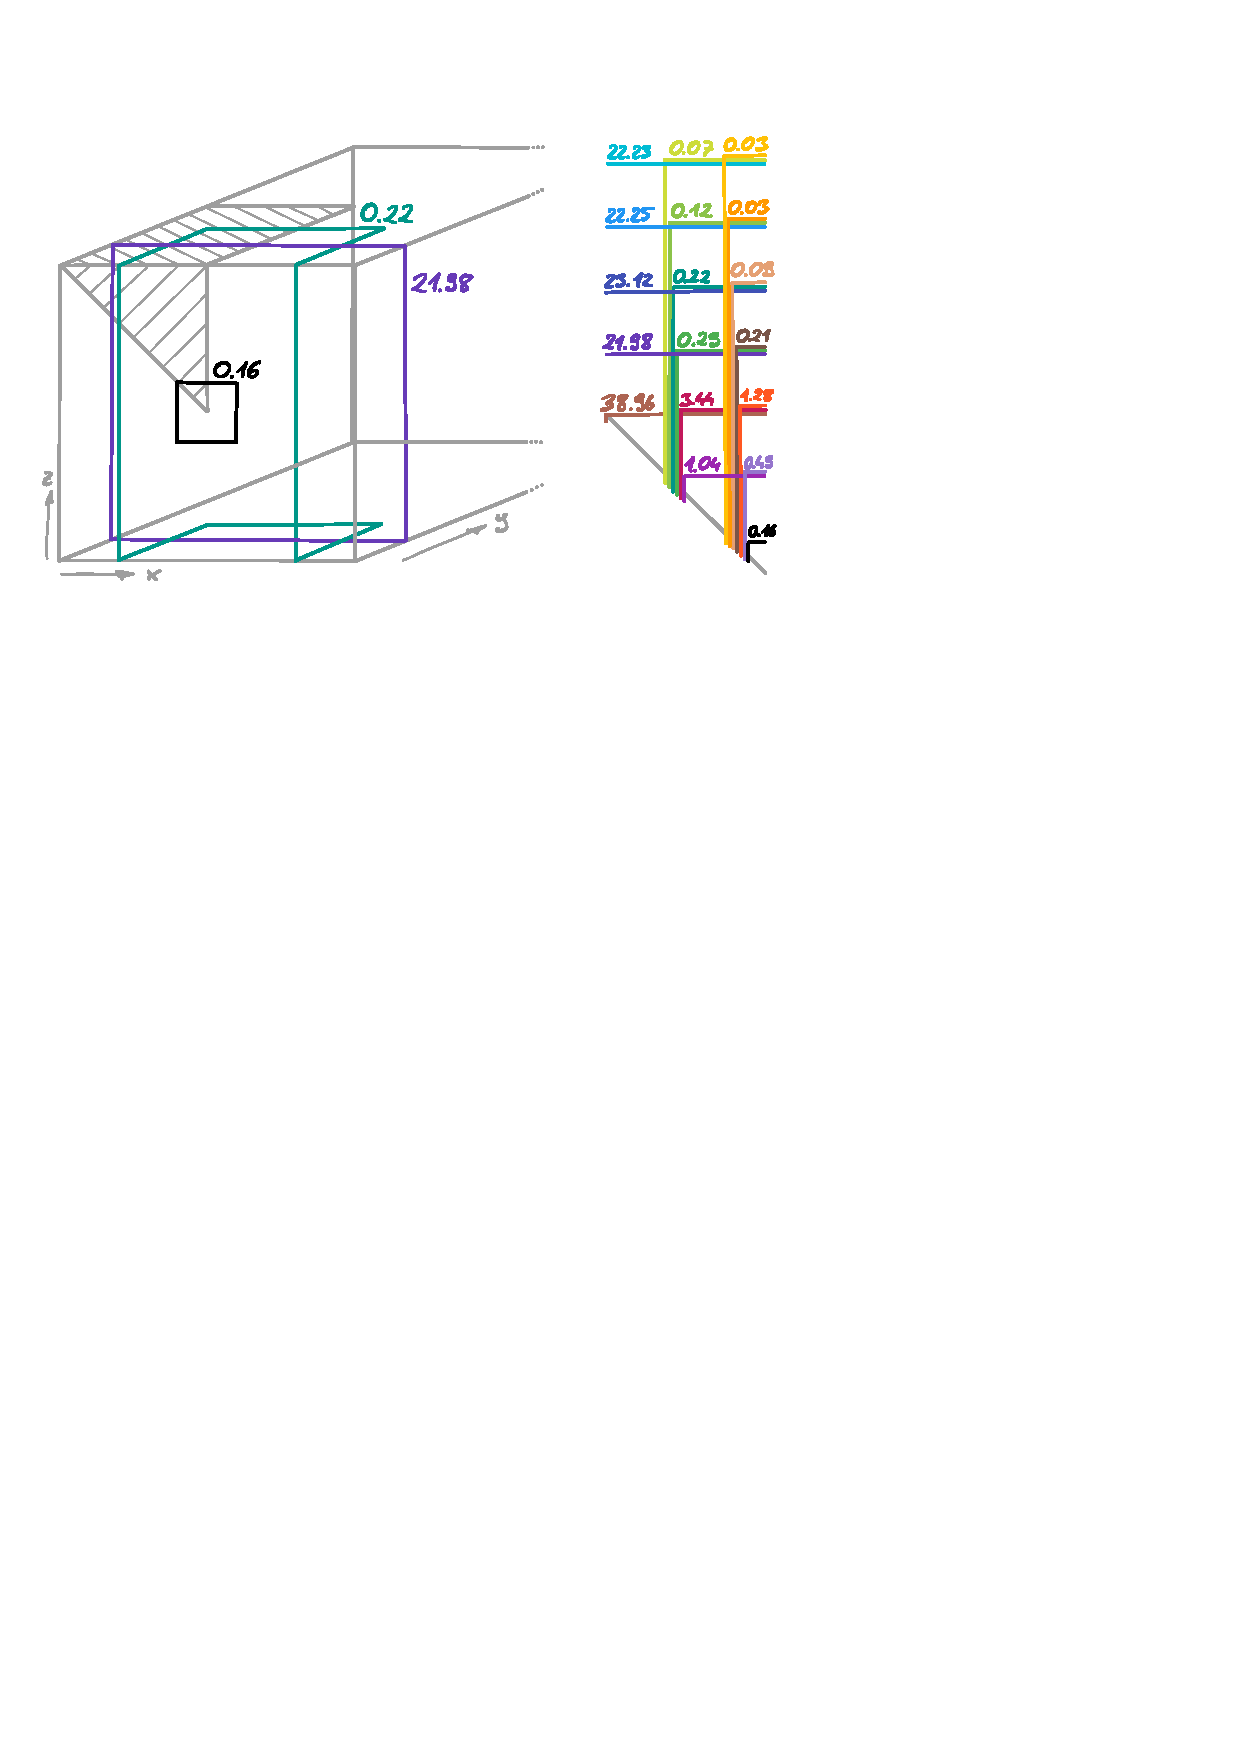
\includegraphics[width=0.9\linewidth]{gfx/prototype/coil_y_decomposition.pdf}
  \caption{The decomposition of the current net of the $y$-coil (Fig.\,\ref{fig:prototype_coil_y_currents}) into current loops. For clarity only a sixteenth part of the system is depicted, all others being identical on the grounds of symmetry. Each loop is indicated with a different colour. The currents are given per \SI{50}{\micro\tesla} of generated field. SHOW WHICH PART IS DEPICTED ON A SMALL 3D DRAWING}\label{fig:prototype_coil_y_decomposition}
\end{figure}

\begin{figure}
  \centering
  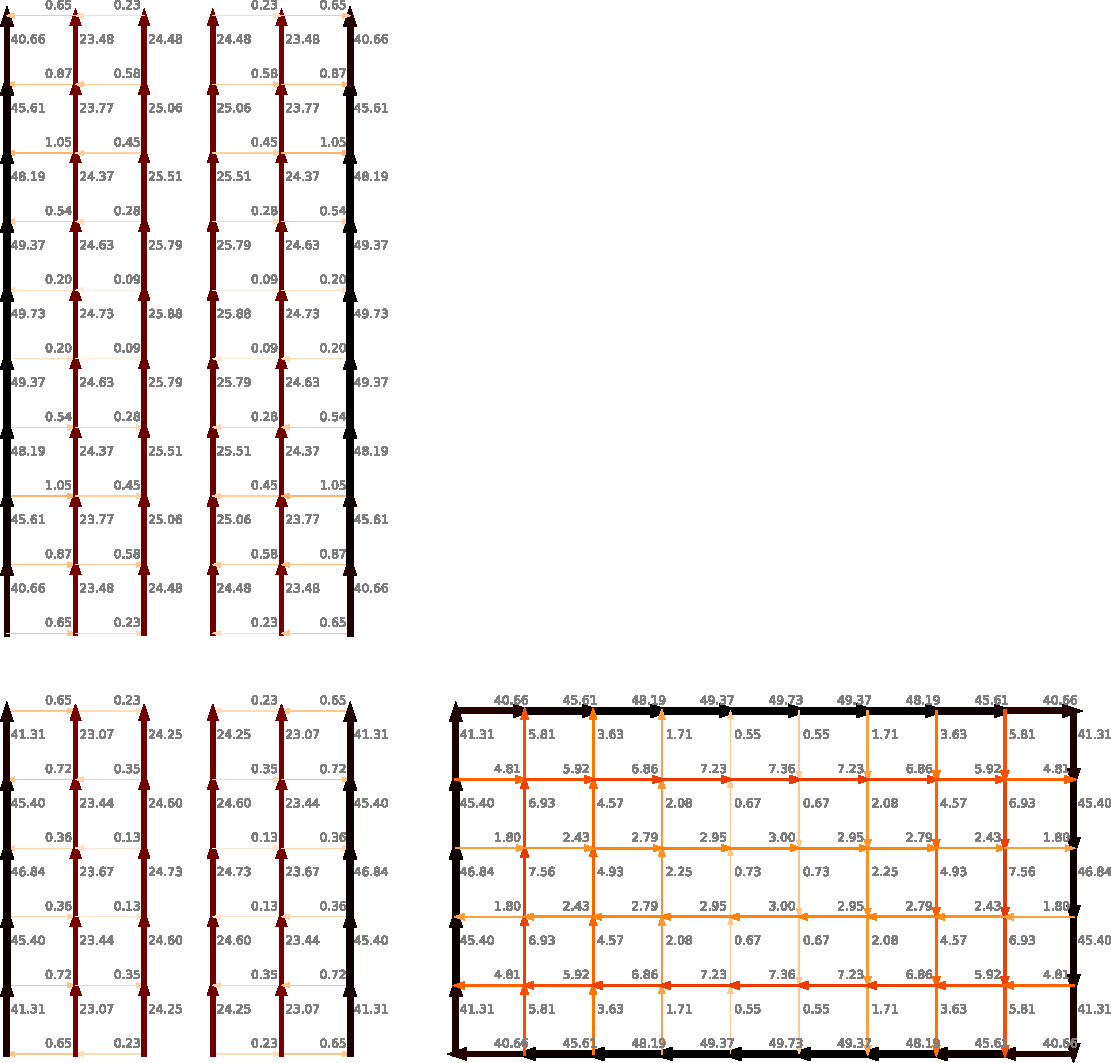
\includegraphics[width=0.9\linewidth]{gfx/prototype/coil_design_x_100uT.pdf}
  \caption{The optimal current net for the $x$ and $z$-coils of the ETH active magnetic field compensation system. Both $5 \times 5$ faces ($y = \mathrm{const}$ planes) are identical and are depicted in the lower-left corner. The rectangular faces perpendicular to the field are depicted to the right, and the ones parallel to it on top. For each segment the current per \SI{100}{\micro\tesla} of generated field is indicated upwards and to the right from its centre.}\label{fig:prototype_coil_x_z_currents}
\end{figure}

% up to the point of the simplification algorithm. Here, The decomposition into loops was done by exploiting symmetries of the system. It is suboptimal in the sense, that there are more windings than there could be.

% Then describe how the coils were designed. The optimized current net is shown in Fig\,\ref{fig:prototype_coil_y_currents} (for the y-coil) and \ref{fig:prototype_coil_x_z_currents} (the x- and z-coils).

% It follows the already described coil design method, up to the point of the simplification algorithm. Here, The decomposition into loops was done by exploiting symmetries of the system. It is suboptimal in the sense, that there are more windings than there could be. The decompositions are depicted in Figs.\,\ref{fig:prototype_coil_y_decomposition} (the y-coil) and \ref{fig:prototype_coil_x_z_decomposition} (the x- and z-coils).

% \begin{figure}
%   \centering
%   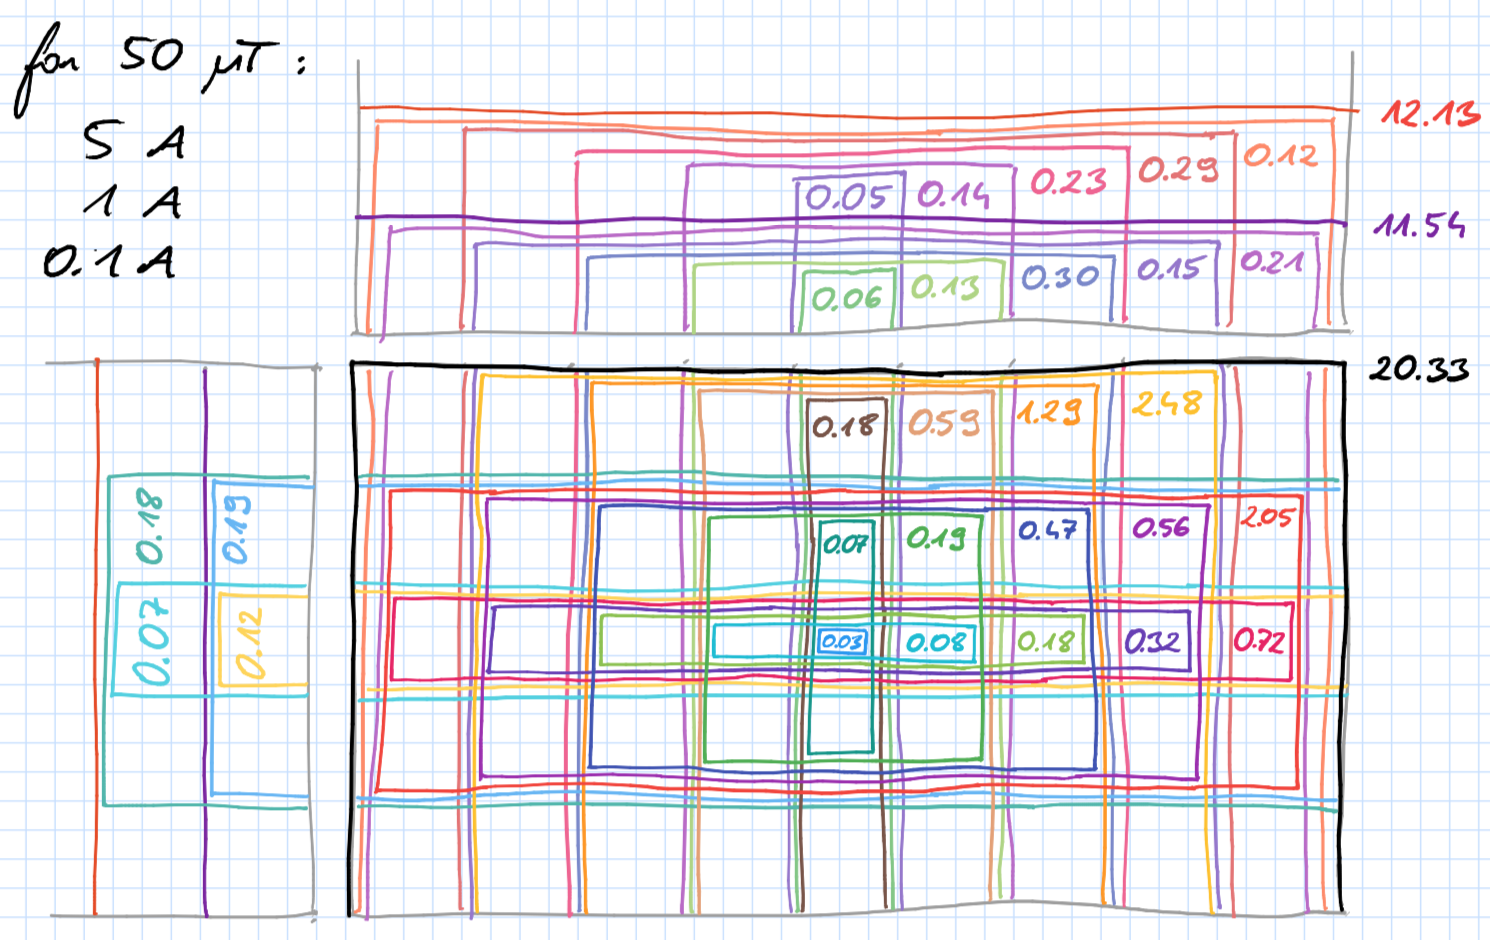
\includegraphics[width=0.9\linewidth]{gfx/prototype/coil_x_z_decomposition.png}
%   \caption{Mention, that it shows\ldots}
%   \label{fig:prototype_coil_x_z_decomposition}
% \end{figure}

\begin{figure}
  \centering
  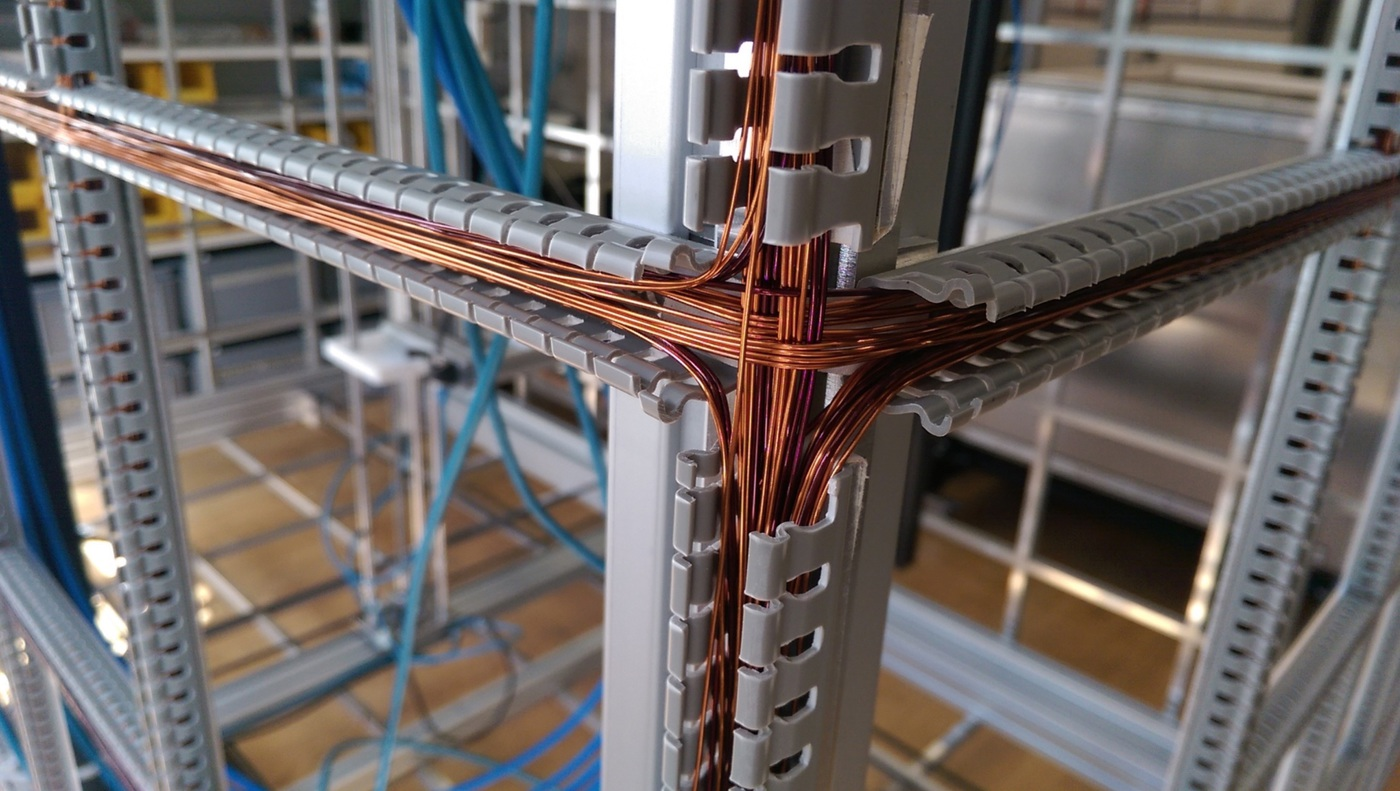
\includegraphics[width=0.9\linewidth]{gfx/prototype/wires_close_up.jpg}
  \caption{A close-up of the wires in the cable channels. Here all three coils for generating the homogeneous fields ($x$, $y$ and $z$) were laid.}\label{fig:prototype_coil_wire_close-up}
\end{figure}

Enameled wire was then laid in the cable channels according to the discretised design. For one current component of a coil, e.g.\ \SI[detect-all = true]{10}{\ampere} in the $x$-coil, a single, long piece of wire was laid, making up all the windings of all loops. For the three coils, each with three components, nine longs wires were laid, in total.
\marginpar{The wire diameter was \SI[detect-all = true]{1}{\milli\meter} for the \num[detect-all = true]{10} and \SI[detect-all = true]{2}{\ampere} wires, and \SI[detect-all = true]{0.8}{\milli\meter} for the \SI[detect-all = true]{0.2}{\ampere} one. The wires were prolonged, when needed.}
A close-up of the wires in the cable channels, for all three coils, is shown in Fig.\,\ref{fig:prototype_coil_wire_close-up}.




\section{Mapping}
\label{sec:prototype_mapping}
The coils were mapped in order to verify that they really produce a field of the required homogeneity. For that purpose a robot has been built: a fluxgate on an xyz-table, controlled with stepper motors. The robot, called a \emph{mapper}, is pictured in Fig.\,\ref{fig:prototype_photo_inside}.

\begin{sidewaysfigure}
  \centering
  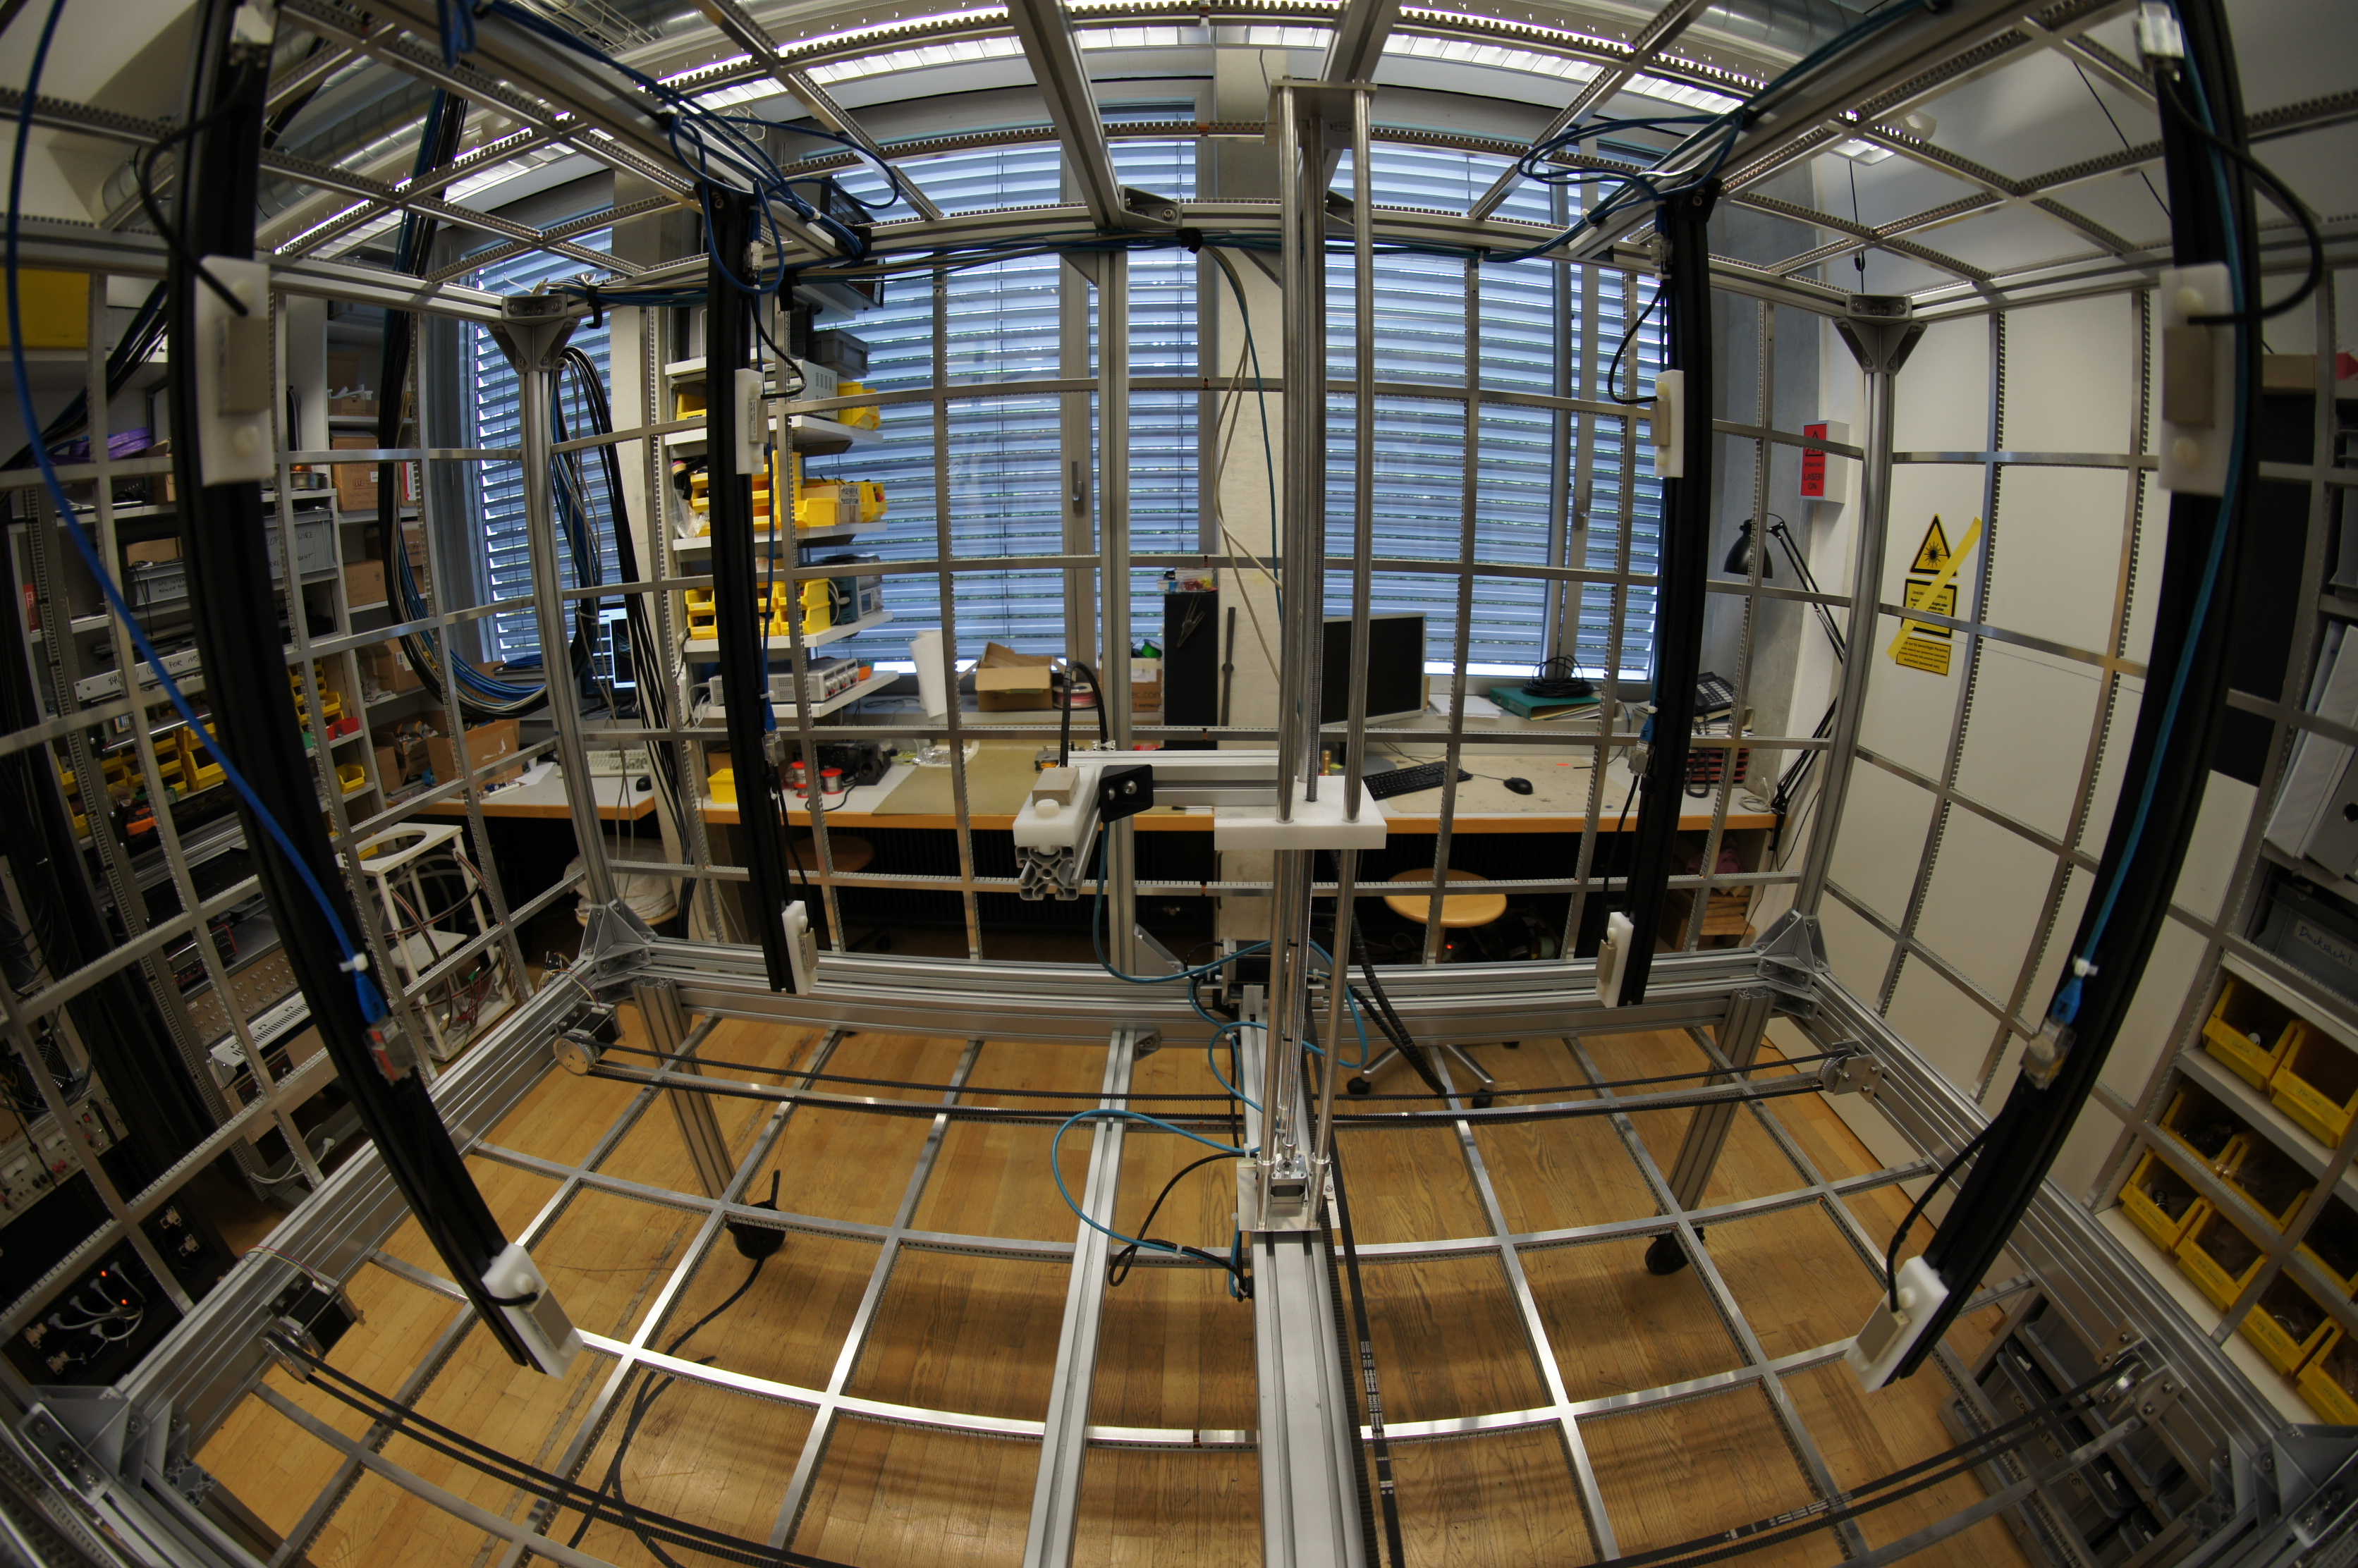
\includegraphics[width=0.75\linewidth]{gfx/prototype/DSC03476.JPG}
  \caption{The inside of the active magnetic field compensation system. In the centre the mapping robot (\emph{mapper}) is visible, with a fluxgate magnetic field sensor mounted to a movable platform. Mounted on black, vertical beams there are eight fluxgates for the active feedback.}\label{fig:prototype_photo_inside}
\end{sidewaysfigure}

A beam seen in the middle of Fig.\,\ref{fig:prototype_photo_inside} could move along the $y$ direction, pulled by two timing belts. The belts were wound around pulleys attached to stepper motors, visible to the left. Along the beam, the $x$ direction, a cart was moved in the same way: a timing belt and a stepper motor. On the cart three vertical rods were attached, with a plastic (POM) platform tightly threaded on them. On the platform there was a fluxgate magnetic field sensor.
\marginpar{In a fluxgate a ferromagnetic core is periodically driven into saturation. When it is not saturated, it is highly permeable and sucks the external magnetic flux in. When saturated, it does not occur. A pickup coil detects the changes in the external flux as it is alternately sucked in and out of the core.}
In the centre of the platform there was an aluminum threaded rod, passing through a threaded hole in it, and mounted to a stepper motor on the cart. As the motor spun the threaded rod, the platform moved vertically, along the $z$ direction.

A simple kind of map was a linear one, whereby the fluxgate was moved along one direction only. A map of the $y$-coil along the $y$ direction, in the middle of $x$ and $z$, is shown in the top part of Fig.\,\ref{fig:prototype_linear_map}. Only the $y$-component of the magnetic field is plotted, the coil was set to produce \SI{50}{\micro\tesla}, and the background field was also mapped and it has been subtracted in the plotted map. The field stayed in a $\SI{\pm 0.2}{\micro\tesla}$ range around the average value.
In the bottom part of Fig.\,\ref{fig:prototype_linear_map} additionally the maps with only the \SI{10}{\ampere} component coil, and with \SI{10}{\ampere} and \SI{2}{\ampere} components coil are shown (for \SI{50}{\micro\tesla} the currents were \SI{5}{\ampere}, \SI{1}{\ampere} and \SI{0.1}{\ampere}). It is interesting to note how much of the field is produced by each of the components. In the middle region the \SI{5}{\ampere}, \SI{1}{\ampere} and \SI{0.1}{\ampere} components produced \SI{86}{\percent}, \SI{11}{\percent} and \SI{3}{\percent} of the \SI{50}{\micro\tesla} field, respectively. At the edge the shares change to \SI{70}{\percent}, \SI{16}{\percent} and \SI{14}{\percent}.

\begin{figure}
  \centering
  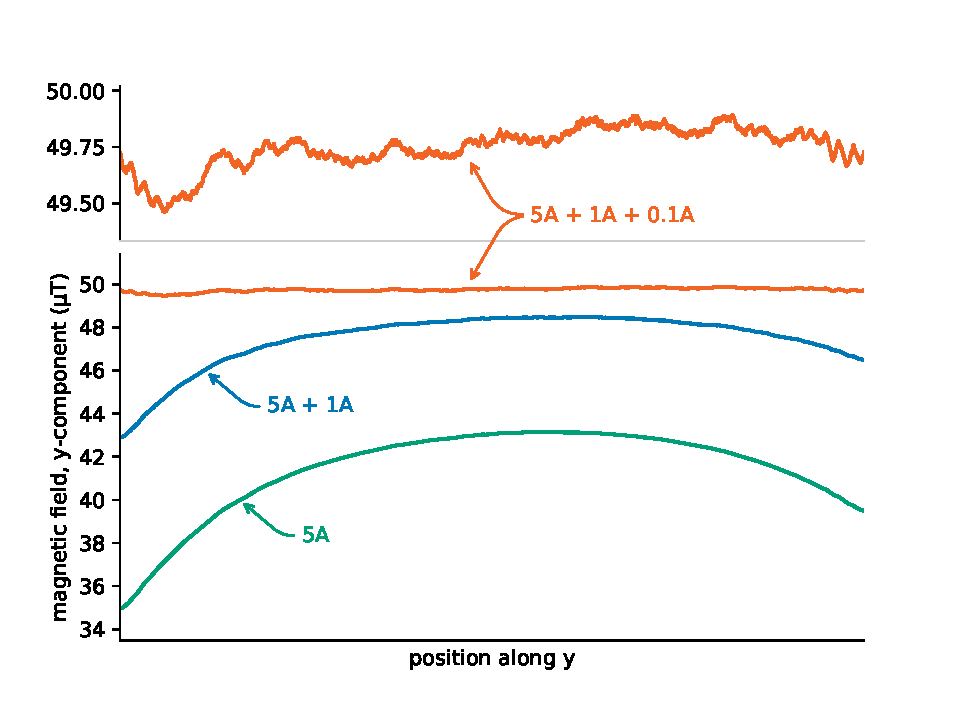
\includegraphics[width=0.8\linewidth]{gfx/prototype/y_scan_all_double.pdf}
  \caption{Linear map of the homogeneous field $y$-coil. The map is along the $y$-direction, in the middle of $x$ and $z$. The $y$-component of the magnetic field is plotted. The green curve depicts the field with only the \SI{5}{\ampere}/\SI{50}{\micro\tesla} wire, the blue with additionally the \SI{1}{\ampere}/\SI{50}{\micro\tesla} one, and the orange, also zoomed in at the very top, all three wires together.}\label{fig:prototype_linear_map}
\end{figure}


%\note{These numbers give also the relative requirements for the components. Five times less stable? Makes no sense\ldots What would the requirements really be? Linearity, for example! Could use worse power supplies.}

\begin{figure}
  \centering
  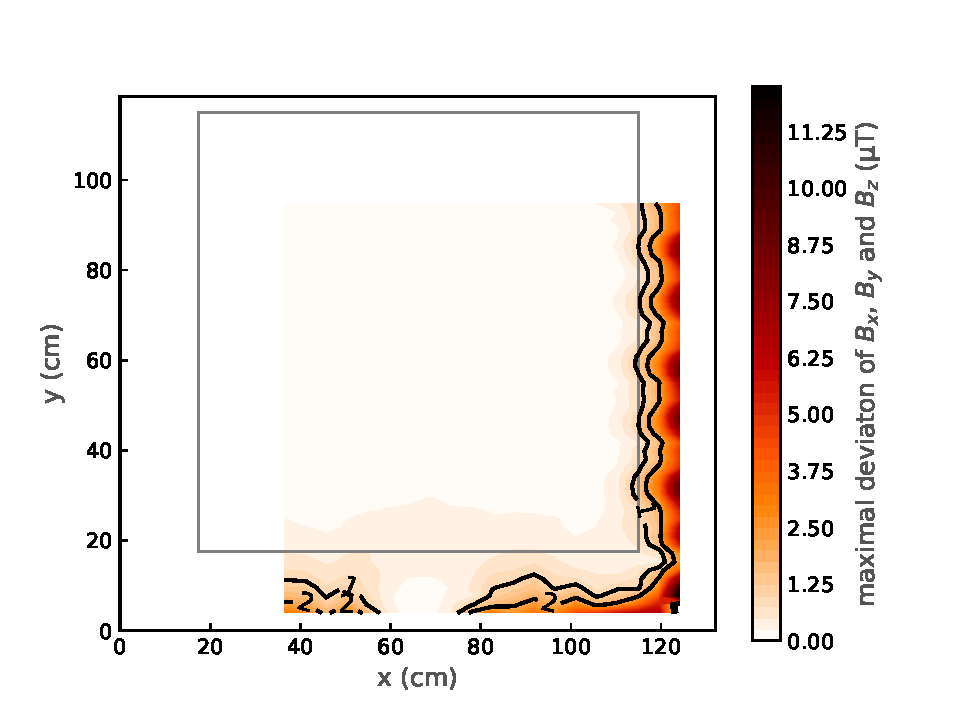
\includegraphics[width=\linewidth]{gfx/prototype/planar_map_Y_max_deviation.pdf}
  \caption{A horizontal map of the $y$-coil, a cut along the middle $xy$-plane. The maximum deviation among all three components of the magnetic field is plotted, i.e.\ in the area enclosed by the \SI{1}{\micro\tesla}~isocountour all components of the field are within \SI{1}{\micro\tesla} from the nominal field (zero for $x$ and $z$, \SI{50}{\micro\tesla} for $y$). Only part of the coil was mapped. The border of the plot corresponds to planes where the wires of the coils are. The border of the fiducial volume is marked with grey lines.}\label{fig:prototype_plane_map}
\end{figure}

Another type of map that was measured was a planar one. A horizontal map, in the middle $xy$-plane, of the $y$-coil is presented in Fig.\,\ref{fig:prototype_plane_map}. The plot shows the maximum deviation among all three components of the magnetic field, i.e.\ in the area enclosed by the \SI{1}{\micro\tesla}~isocountour all components of the field are within \SI{1}{\micro\tesla} from the reference field. The reference field would ideally be zero for $x$ and $z$, and \SI{50}{\micro\tesla} for $y$. In reality the sensor's axis were not perfectly aligned with the ones of the system, causing the $x$ and $z$ components to be non-zero, and $y$ to be smaller. The reference field was set as the average field in the area of the highest homogeneity in the middle of the map. Within the fiducial volume the field deviated by no more than \SI{2}{\percent} or \SI{1}{\micro\tesla} for a \SI{50}{\micro\tesla} field, as expected. Maps of the other coils gave similar results.
%\mnote{Need to be clear about the specification---it wasn't supposed to be 2\% EVERYWHERE! Maybe bring forward the specification plot that decided on the grid size?}




\section{Control System}
In this section the hardware stack used to measure and control the magnetic fields is described.
% Before proceeding to discuss the active stabilisation system, we devote a section to the hardware. These are technical details, but for the more tech-savvy of the readers having the hardware setting given first may ease following the discussion.
In an active magnetic field stabilisation system a change in the magnetic field is detected with an array of sensors, an appropriate response is calculated and applied by driving a change in currents flowing in the coils. The feedback loop is closed through the air when the sensors detect the change in the field caused by the coils.

In the system at ETH the field was measured with eight fluxgates, visible in Fig.\,\ref{fig:prototype_photo_inside}. They were mounted in a way that they make up corners of a cube of approximately \SI{90}{\centi\meter} side length.
The sensors were Stefan Mayer Instruments FLC3--70 three-axis fluxgates, $\SI{\pm 200}{\micro\tesla}$ range, \SI{1}{\kilo\hertz} bandwidth, $\pm \SI{1}{\percent} \pm \SI{0.5}{\micro\tesla}$ accurate.
They were powered with an in-house--built $\SI{\pm 5}{\volt}$ power supply. The outputs of the fluxgates were $\SI{\pm 5}{\volt}$ signals proportional to the magnetic field.
The analogue signals were directly digitised with Beckhoff EL3602 24-bit differential analogue-to-digital converters (ADCs). The digital information was collected in software running on a PC computer.

\marginpar{The main julia program published the data on a \texttt{ZMQ} \texttt{PUB} socket. The data were stored with a separate \texttt{julia} program, collecting the data on a \texttt{ZMQ} \texttt{SUB} socket. Similarly, the plotting program was separate, written in \texttt{Python}.}
The software stack, running under OpenSUSE Linux, consisted of a low-level Ethercat driver~\cite{etherlabcode} on top of which a custom program, written in \texttt{julia}~\cite{julia}, was running.
This setup was optimised for high flexibility and close-to-zero turnaround time in development. In particular, it was possible to develop the software interactively \emph{while} the system was running. The main task of the program was to keep evaluating the optimal response for the measured magnetic field changes. The optimal response, the new currents to be applied to the coils, was sent to the digital-to-analogue converters (DACs). Besides, the data were recorded and plotted on-line. 

The DACs were 16-bit Beckhoff EL4134. The signals were then amplified with an array of four-quadrant SERVOWATT amplifiers, configured to amplify the $\SI{\pm 10}{\volt}$ input to a current output. For each coil the three stages were: DCP260/30A configured with a $\SI{\pm 10}{\ampere}$ output, DCE50/30A with $\SI{\pm 2}{\ampere}$ one and DCE10/30A with $\SI{\pm 0.4}{\ampere}$ one. The currents were then directly fed into the coils.

\begin{SCfigure}
  \centering
  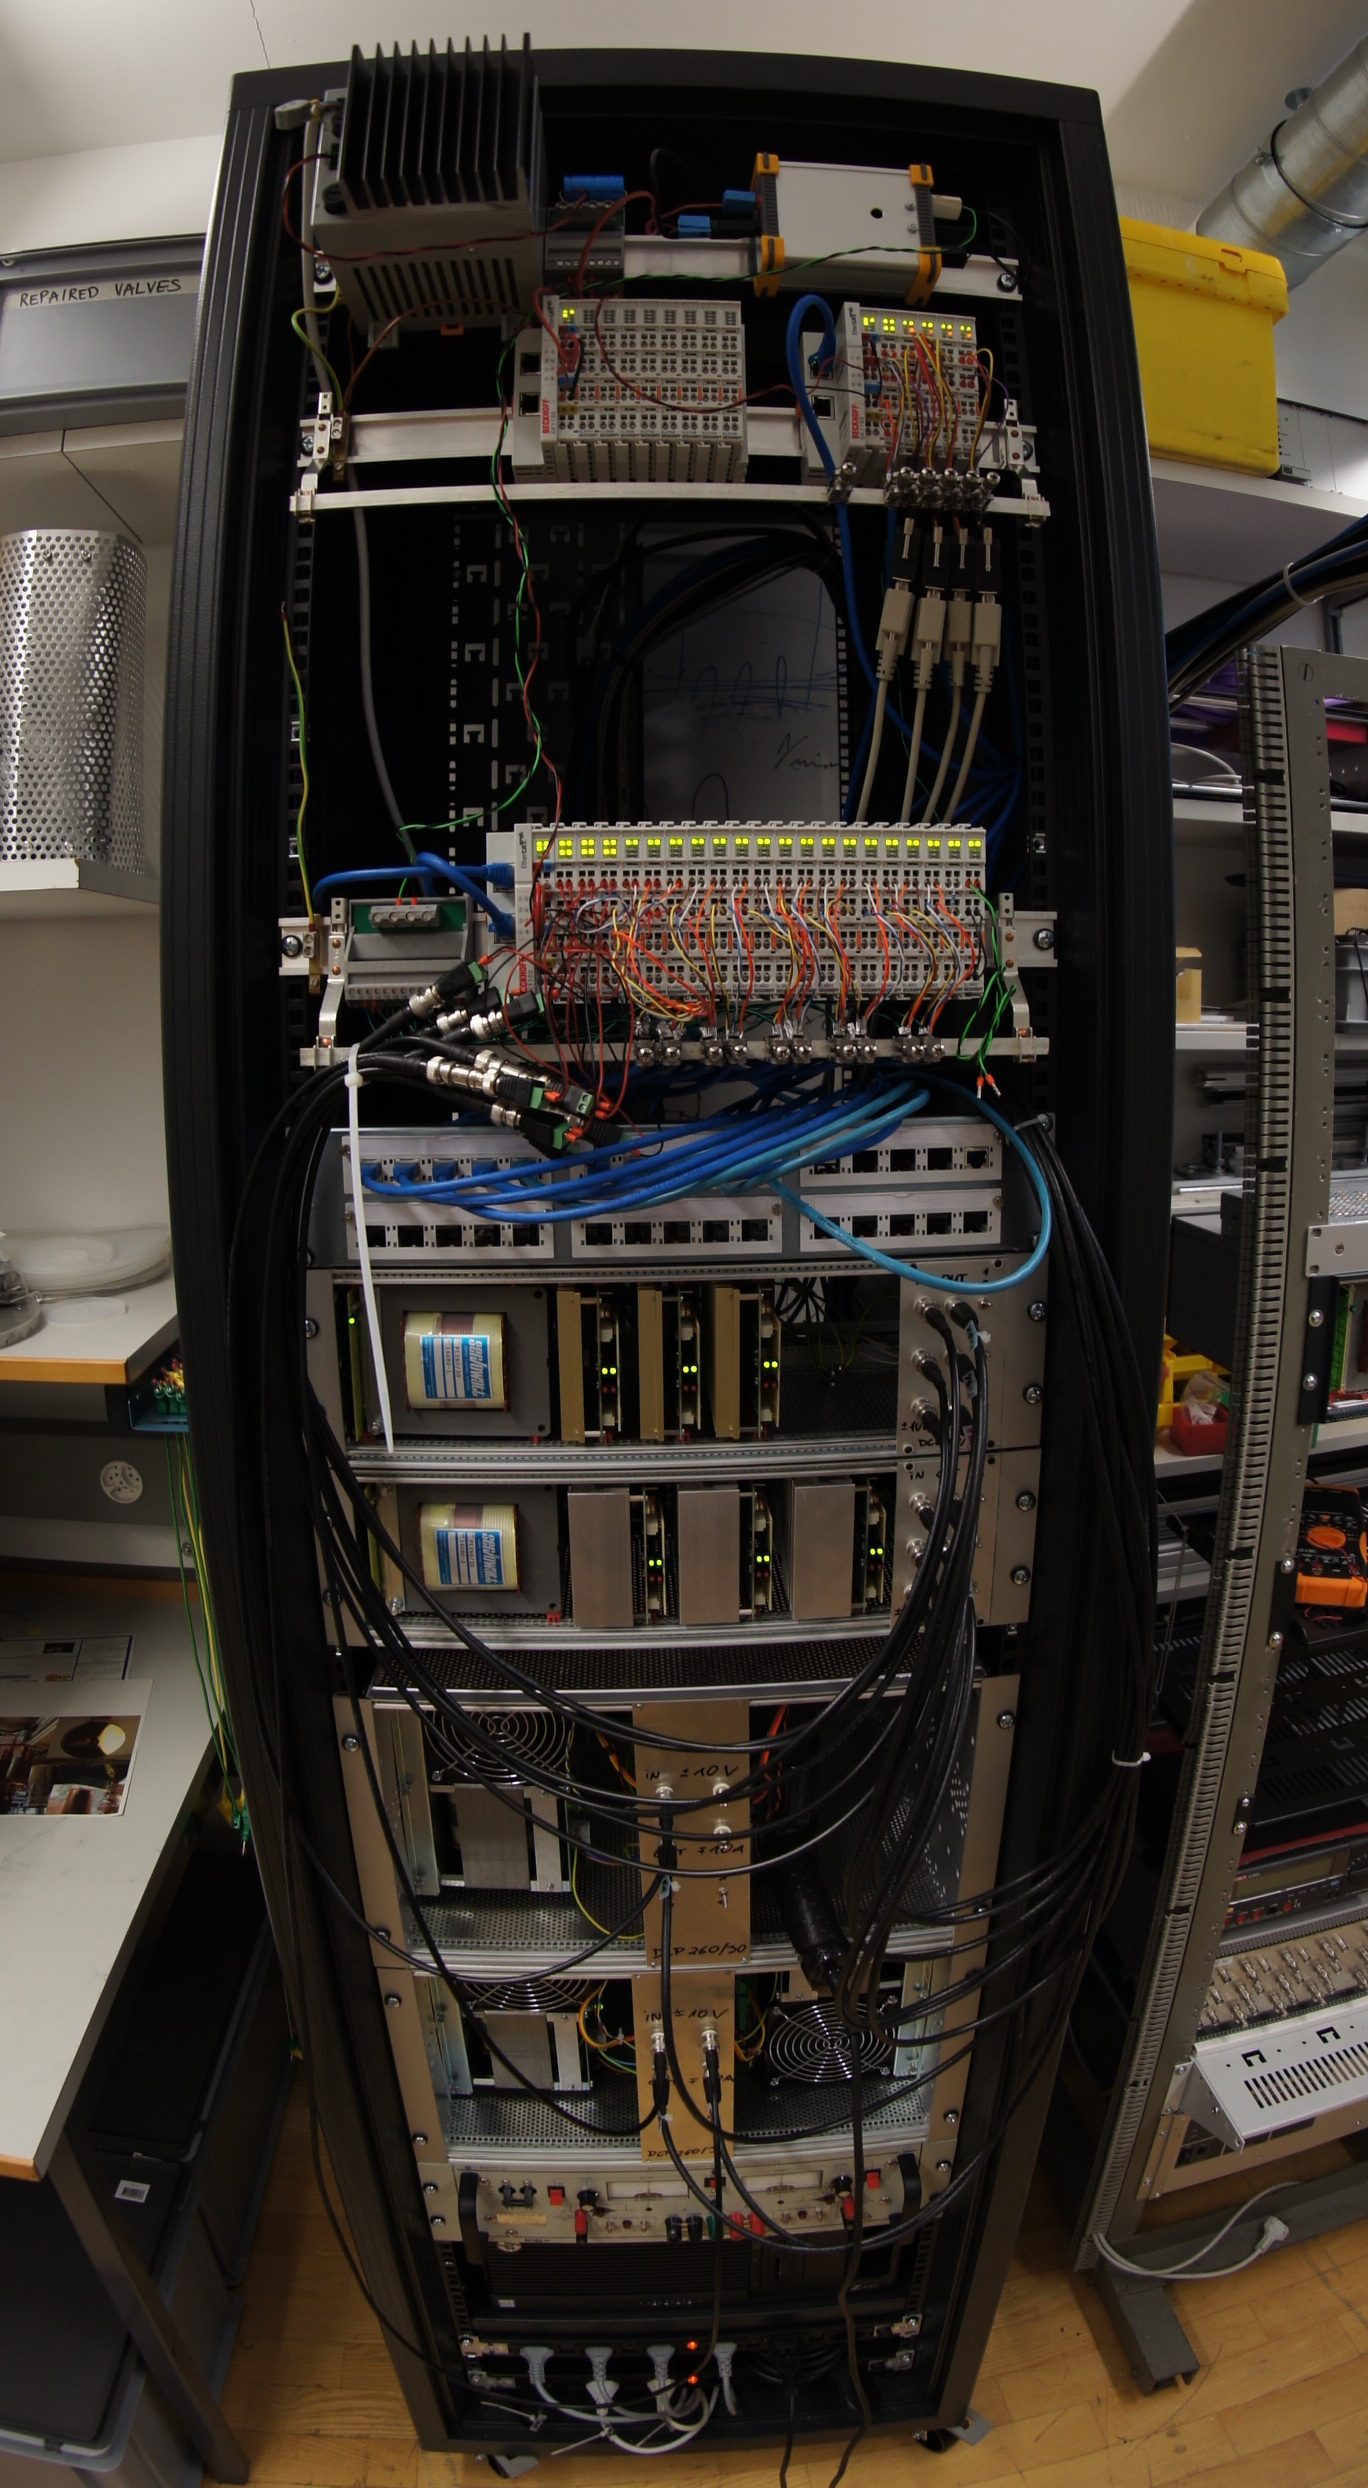
\includegraphics[width=0.6\linewidth]{gfx/prototype/DSC03477_cropped.jpeg}
  \caption{The 19-inch cabinet hosting the electronics for the active magnetic field stabilisation system. From top: a \SI{24}{V} power supply for the Beckhoff EtherCAT clamps and in-house--built $\SI{\pm 5}{\volt}$ power supply for the fluxgates; spare EtherCAT clamps and control system for the mapper; a large array of EtherCAT DACs and ADCs for the active stabilisation system; breakout panel for the fluxgate cables (RJ-45 plugs); subrack with $\SI{\pm 0.4}{\ampere}$ amplifiers; subrack with $\SI{\pm 2}{\ampere}$ amplifiers; two subracks with $\SI{\pm 10}{\ampere}$ amplifiers; a general-purpose Kepco $\SI{\pm 20}{\volt}$ $\SI{\pm 20}{\ampere}$ four-quadrant amplifier; the PC.}\label{fig:prototype_photo_daq}
\end{SCfigure}

The hardware was hosted in a 19-inch cabinet, pictured in Fig.\,\ref{fig:prototype_photo_daq}. A detailed list of the components can be found in the Figure's caption. All these components, additionally to the coils themselves, were used to run the active magnetic field compensation.




\section{The feedback matrix}
The system utilises the feedback matrix, as described in Ch.\,\ref{ch:nedm_sfc}. The magnetic field measured by each of the 24 sensors is linear with the currents in the three coils. All readouts, gathered in a vector $\mathbb{B}$ (dimension~24) can be written as a linear combination of the currents in the coils $\mathbb{I}$ (dimension~3):
\marginpar{We use the symbol $\mathbb{B}$ for the values measured by the sensors to distinguish it from $\bm{B}$, which is used to denote the magnetic field in the whole space.}
\begin{equation}
  \label{eq:SFC_matrix_model}
  \mathbb{B} = M \mathbb{I} + \mathbb{B}_0 \ ,
\end{equation}
where $\mathbb{B}_0$ is the free offset. The matrix of proportionality constants $M$, dimension $24 \times 3$, is the central element of the active magnetic field compensation.

Let us recall the discussion of the PSI system's matrix in Sec.\,\ref{fig:nEDM_SFC_matrix}. There, we pointed out that its high condition number, and the need for regularisation, was due to the geometry of the system. In particular, some linear combinations of the coils created high-order fields which, despite high currents, had little influence on the sensors' readout.
% The matrix of the PSI system and its properties were thoroughly discussed in Sec.\,\ref{fig:nEDM_SFC_matrix}.
There is a fundamental difference between the matrix of the PSI's system and the one of the next generation's one. The PSI matrix was not known a priori. The system was constructed and the matrix was measured as the system's property.
% This could be considered as the reason that the matrix was ill-conditioned and the system required regularisation and PI control to be stable.
Conversely, the new system takes the matrix into account already at the design phase. The coils are designed to produce magnetic field corresponding to the terms of the cartesian harmonic expansion of the field.
This ensures that they are orthogonal to one another. We expect, by design, the matrix to have the condition number equal to \num{1}. It has been measured to be \num{1.064} with the three coils for the homogeneous components.

% \note{Put a figure about the measurement of the matrix?}

The active magnetic field compensation system constructed at ETH implemented a new way of measuring the matrix. The procedure changed currents in all the coils simultaneously, shortening the duration of the procedure, and could measure in close-to-zero field conditions. To measure the matrix, the space spanned by all the coils was considered. In this case it was three-dimensional: the current in the $x$-coil, in the $y$-coil and in the $z$ one. A point in this space corresponded to one configuration of the currents in the coils. A set of points on an n-sphere in this space was picked and all currents were changed simultaneously, making their way from one point to another. As the currents were changed, the measurements of the sensors were recorded. Then, for each readout channel, 24 in total, a linear model was fitted to estimate the proportionality constants between the readout and the currents in the coils:
\begin{equation}
  \label{eq:SFC_matrix_linear_fits}
  B_i = B_i^0 + \sum_{j=x,y,z} M_{i,j} \, I_j \ ,
\end{equation}
where $B_i$ is the readout channel ($i$ going from 1 to 24), $I_j$ are the currents in the coils ($j$ going over $x$, $y$ and $z$) and $M_{i,j}$ is the matrix of proportionality constants---the feedback matrix. $B_i^0$ is the free offset vector---the background field.
% \note{Sort out the indexes, which is which.}

If the system is perfectly linear it does not matter where in the current-space the n-sphere is located, nor how large it is (though larger ones give more precise estimates per point). We expect, however, non-linearities to appear in the presence of a mu-metal shield inside the system.
\marginpar{It is possible to fit the linear model and estimate the uncertainty of the matrix elements \emph{while} measuring; the measurement can be stopped when the uncertainty drops below a threshold.}
In that case it is preferable to measure the matrix in the vicinity of the point where the system is later operated. Motivated by this, the following procedure of the matrix measurement was employed: First an n-sphere centred at n-zero and a radius of \SI{50}{\micro\tesla} was chosen. Then the system walked over ten random points on the sphere, taking two seconds to go from one to the next (\SI{20}{\second} in total).
This gave the first estimate of the matrix. The next sphere was chosen to be centred around the zero field. This is the optimal, in the least-squares sense, solution of Eq.\,\ref{eq:SFC_matrix_model} with $\mathbb{B} = 0$:
\begin{equation}
  \label{eq:SFC_zero_field_requirement}
  \mathbb{I}_\text{zero-field} = - M^\dagger \, \mathbb{B}_0 \ ,
\end{equation}
where $\mathbb{B}_0$ is the free offset from Eq.\,\ref{eq:SFC_matrix_linear_fits} and $M^\dagger$ is the Moore-Penrose pseudoinverse of the matrix $M$. This gave the second estimate of the matrix. Finally, the measurement was repeated with a sphere again centred at zero, but with a smaller radius of \SI{1}{\micro\tesla}. The procedure was developed for a system with mu-metal. In the case of a linear air system all consecutive estimates of the matrix were almost the same.
% \note{Hopefully I still do get to measure the matrix with the $\upmu$-metal cube inside. Then I will describe it here.}

\begin{figure}
  \centering
  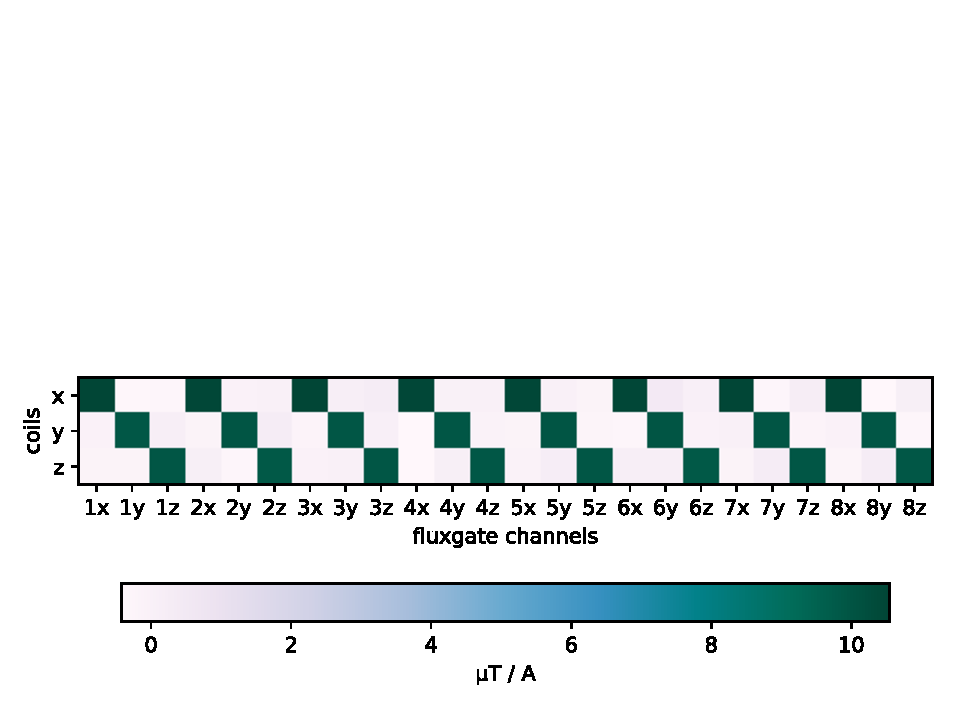
\includegraphics[width=.9\linewidth]{gfx/prototype/SFC_matrix_green.pdf}
  \caption{The measured feedback matrix of the active magnetic field compesnation system. The sensors were mounted $\approx\SI{20}{\centi\meter}$ away from the coil surface. The values are microteslas of field per \SI{1}{\ampere} in the strongest coil (\SI{1}{\ampere} and \SI{0.1}{\ampere}) in the others.}\label{fig:prototype_feedback_matrix}
\end{figure}

The matrix measured with the sensors mounted $\approx\SI{20}{\centi\meter}$ away from the coil surface is presented in Fig.\,\ref{fig:prototype_feedback_matrix}. The differences between the non-zero elements of different fluxgates are under 1\%, as expected from the design and the field map (Fig.\,\ref{fig:prototype_plane_map}). The condition number of the matrix is \num{1.064}.
% A typical measured matrix is\ldots Estimate the field inhomogeneity right away from it! Give two at two distances, maybe? The one I looked at has around 0.5\% std homogeneity at the sensors' positions.

% Then continue to analyse the matrix. Discuss the SVD decomposition and its singular values. Or is it the right place to do it here?



\section{The feedback algorithm}
The feedback was based on calculating the optimal solution of the Eq.\,\ref{eq:SFC_matrix_model} in each step. In the $n$th iteration (the iteration index marked on top) the equation is:
\begin{equation}
  \mathbb{B}^n = M \mathbb{I}^n + \mathbb{B}_0^n \ .
\end{equation}
In the next iteration we want the field to be equal to the target field (which we allow to be any): $\mathbb{B}^{n+1} \overset{!}{=} \mathbb{B}_\text{target}$, which leads to the following requirement for the next currents:
\begin{align}
  \mathbb{I}^{n+1} &=
    M^\dagger \left( \mathbb{B}_\text{target} - \mathbb{B}_0^{n+1} \right) \nonumber \\
    &\approx M^\dagger \left( \mathbb{B}_\text{target} - \mathbb{B}_0^{n} \right) \nonumber \\
    &= M^\dagger \left( \mathbb{B}_\text{target} - \mathbb{B}^n + M \mathbb{I}^n \right) \nonumber \\
    &= M^\dagger \left( \mathbb{B}_\text{target} - \mathbb{B}^n \right) + M^\dagger M \mathbb{I}^n \nonumber \\
    &= M^\dagger \left( \mathbb{B}_\text{target} - \mathbb{B}^n \right) + \mathbb{I}^n \ . \label{eq:current_update}
\end{align}
By defining $\Delta\mathbb{I}^n := \mathbb{I}^{n+1} - \mathbb{I}^{n}$ and $\Delta\mathbb{B}^n = \mathbb{B}^n - \mathbb{B}_\text{target}$ we obtain the intuitive rule for the current update:
\begin{equation}
  \Delta\mathbb{I}^n = - M^\dagger \Delta\mathbb{B}^n \ .
\end{equation}
A careful reader may be alarmed by the approximation $\mathbb{B}_0^{n+1} \approx \mathbb{B}_0^{n}$. It is an unfortunate necessity, for the calculation needed to be performed just before the iteration $n+1$, when $\mathbb{B}_0^{n+1}$ is not yet known. In other words, the correction was delayed by one iteration. This introduced a lag in the system and motivated high feedback frequencies.

\begin{figure}
  \centering
  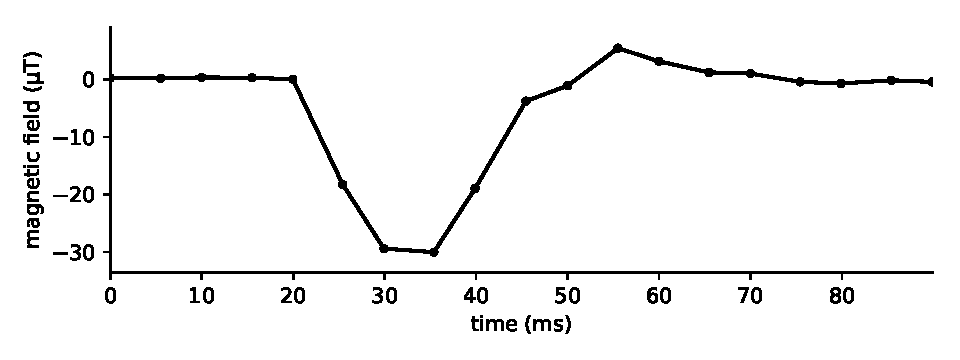
\includegraphics[width=.9\linewidth]{gfx/prototype/SFC_step_response.pdf}
  \caption{The reaction of the active magnetic field compensation to a step change in the magnetic field ($\approx \SI{30}{\micro\tesla}$ in \SI{5}{\milli\second}). The system was running at a rate of \SI{200}{\hertz}. Each dot marks one iteration.}\label{fig:prototype_step_response}
\end{figure}

In practice, the system had a delay of more than one iteration. Although the system was operated at \SI{200}{\hertz}, the quickest turnaround was three cycles, \SI{15}{\milli\second}. This was tested by applying a pulse on an DAC channel and observing the response on a directly connected ADC channel. Knowing that the magnetic field information is delayed, it was crucial to delay the current information, too, so that Eq.\,\ref{eq:current_update} became:
\begin{equation}
  \mathbb{I}^{n+1} = M^\dagger \left( \mathbb{B}_\text{target} - \mathbb{B}^{n-2} \right) + \mathbb{I}^{n-2} \ .
\end{equation}
Without accounting for the delay the system would spontaneously destabilise. In Fig.\,\ref{fig:prototype_step_response} a response of the the system to a step-like change of the magnetic field is plotted. Note, how the system's reaction is delayed by three iterations.

% \note{A paragraph (or a margin note) comparing the feedback algorithm to the old one. Requires no parameters, any field may be the target field.}

% \note{Has been tested with the big system, but it did not outperform in terms of stability (do I have a plot to prove that?). Nick Schwegler's project report! I could just cite it here, it was inconclusive. But for sure I can say it.}




\section{Dynamic stabilisation}
The dynamic stabilisation was tested with a strong permanent magnetic dipole. It was build out of two extremely strong neodymium magnets (\SI{200}{\kilo\gram} force when attached to iron) connected with an iron rod. The dipole was moved by hand several meters from the system causing a magnetic field disturbance.

% \mnote{Need to put the details of the geometry of the fluxgates here. Eight fluxgates on the corners of a cube of \ldots size.}

\begin{figure}
  \centering
  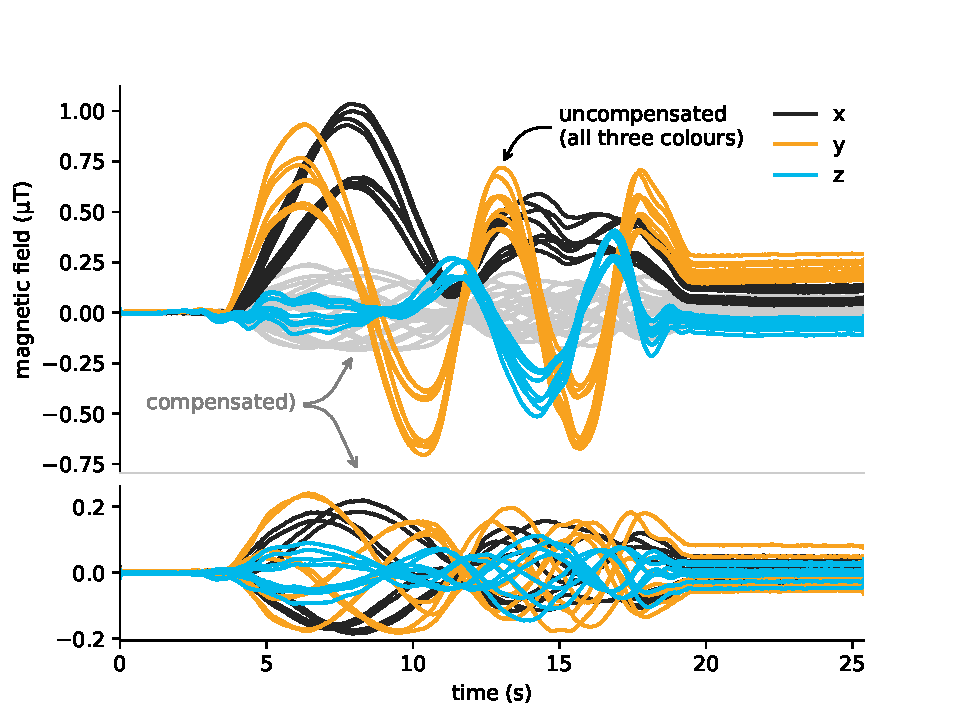
\includegraphics[width=.8\linewidth]{gfx/prototype/compensated_7_5m_double.pdf}
  \caption{Field variations caused by a rotating dipole \SI{7.5}{\meter} away.
  The upper part shows in colours corresponding to the spatial directions the uncompensated field $\mathbb{B}_0$ for all eight sensors, calculated according to Eq.\,\ref{eq:uncompensated_field}. Each line is one sensor. The compensated field $\mathbb{B}$ is depicted in grey in the upper part and is enlarged in the lower part of the plot, in colour. The curves have been smoothed for clarity.}\label{fig:prototype_compensation_time}
\end{figure}

The result of the compensation of the dipole being rotated \SI{7.5}{\meter} away from the system's centre are plotted in Fig.\,\ref{fig:prototype_compensation_time}. The upper part of the plot shows the field as it would be registered without compensation $\mathbb{B}_0$, calculated according to Eq.\,\ref{eq:SFC_matrix_model}:
\begin{equation}
  \label{eq:uncompensated_field}
  \mathbb{B}_0 = \mathbb{B} - \mathbb{M} \mathbb{I} \ .
\end{equation}
% The three colours correspond to the three spatial components ($x$, $y$, $z$). Each line is one sensor.
In the bottom part the actually measured field $\mathbb{B}$ is depicted. The amplitude of the changes was reduced from around \SI{1.75}{\micro\tesla} to \SI{0.4}{\micro\tesla} (factor four). Yet, the variation is not mitigated completely and the reason in quite fundamental.

Take a look on the orange lines in the upper part of Fig.\,\ref{fig:prototype_compensation_time}, each representing the readout of a different sensor in the $y$ direction. They do not overlap, which means that the field change was not homogeneous (which, of course, would be the same everywhere). The coils of the system, being able to generate only homogeneous fields, can only compensate the homogeneous part. Graphically it may be explained in the following way: each of the coils coil can keep all lines in one of the colours (one spatial component) steady, but it cannot bring them closer together (homogenise the field). This is what can be observed on the right-hand side of Fig.\,\ref{fig:prototype_compensation_time}. There lines are centred around zero, but their spread within one colour (spatial component) is not reduced. In order to do that, coils producing higher-order fields would be required.
% After all, the active compensation can compensate only as much as it can.

\begin{figure}
  \centering
  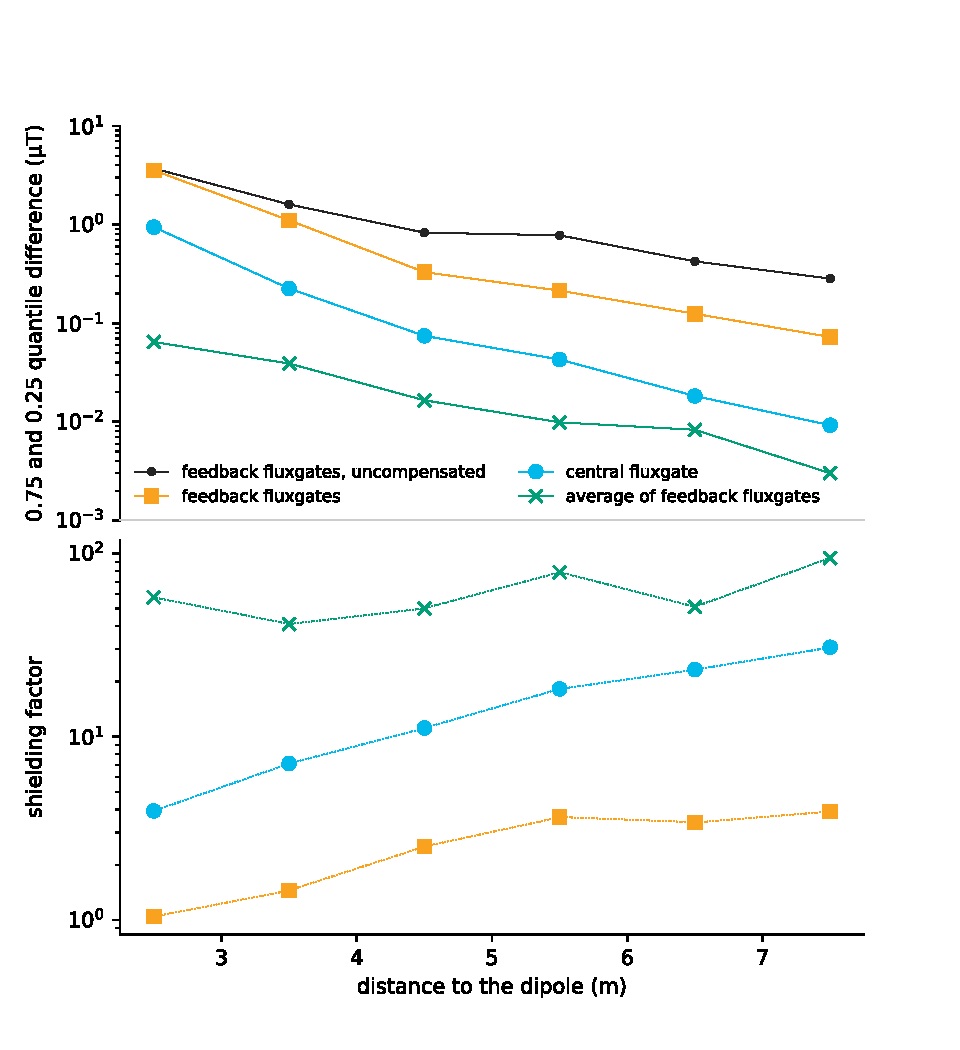
\includegraphics[width=0.85\linewidth]{gfx/prototype/big_magnet_performance_shielding_factor.pdf}
  \caption{Performance of the active compensation system shielding a dipole disturbance, as a function of the distance to it. Upper part: the amplitude of the field variations, measured as the difference between the 75th and 25th quantiles, as uncompensated (black), compensated seen by the feedback sensors (orange), a non-feedback sensor in the centre (blue) and the numerical average of the feedback sensors (green). Lower part: the shielding factor, defined as the ratio of the curves in the plot to the left to the uncompensated variation.}\label{fig:prototype_compensation}
\end{figure}

The amplitude of the variations seen in Fig.\,\ref{fig:prototype_compensation_time} can be quantified as the difference between 75th and 25th quantiles of the readouts. This measure is plotted in the upper part of Fig.\,\ref{fig:prototype_compensation} as the function of the distance between the dipole disturbance and the centre of the system. The uppermost curve, black, is the uncompensated field $\mathbb{B}_0$. The orange one below is the compensated field seen by the feedback sensors $\mathbb{B}$ (the bottom part of Fig.\,\ref{fig:prototype_compensation_time}). We observe that the compensation improved with the distance to the dipole, as the field became weaker and more homogeneous. In the bottom of the figure the ratio of the two curves, called the \emph{shielding factor}, is plotted in orange.

The next curve, blue, corresponds to the field measured by a sensor placed in the middle of the system. There the system compensates 1st-order changes (because they are anti-symmetric with respect to the centre). It suggests that the difference to the shielding factor for the feedback sensors, a factor three, can be attributed to the uncompensated variations of 1st-order gradients. Furthermore, it suggests that if the system would be extended by a addition of 1st-order coils the shielding factor for the feedback sensors (in the whole volume) would be as good as for the centre.

The last, red, curve depicts the variations seen in the average readout of the feedback fluxgates. An ideal system should compensate it perfectly, regardless of the shape of the field changes. Yet, the shielding factor for this measure was around 50. It also did not depend on the distance to the dipole (homogeneity of the field), suggesting that it is a property of the compensation system itself. The dominant factors are probably the finite reaction time and the inhomogeneity of the field created by the compensation coils (the inhomogeneity is around 1\%). Even if the changes of the field were similar in magnitude and pace to the ones discussed, but perfectly homogeneous, this system is not likely to compensate them better then by a factor of 50.




\section{Long-term Stability}
\marginpar{In the PSI environment periods of strong magnetic field changes, tens of microteslas over an hour when nearby magnets ramp, were interleaved with ones of high stability---\SI[detect-all = true]{10}{\nano\tesla} at \SI[detect-all = true]{10}{\second} at night (Fig.\,5.3 in Ref.\,\cite{Franke2013}).}
We have just discussed how the active magnetic field compensation system can stabilise the field in the case of strong variations. However, the system's internal stability was inevitably finite. In conditions, where the environmental magnetic field would be more stable than than, the system would effectively destabilise the field. In this section we will discuss where the limit of the stability was.

As the measure of stability we use the \emph{Allan deviation}, a special case of the M-sample variance, defined originally by the Eq.\,11 in Ref.\,\cite{Allan1966}, with $N=2$ and $T = \tau$.
It has a simple interpretation: for a given integration time $\tau$ it gives the RMS variation from one integrated sample to the next.

\begin{figure}
  \centering
  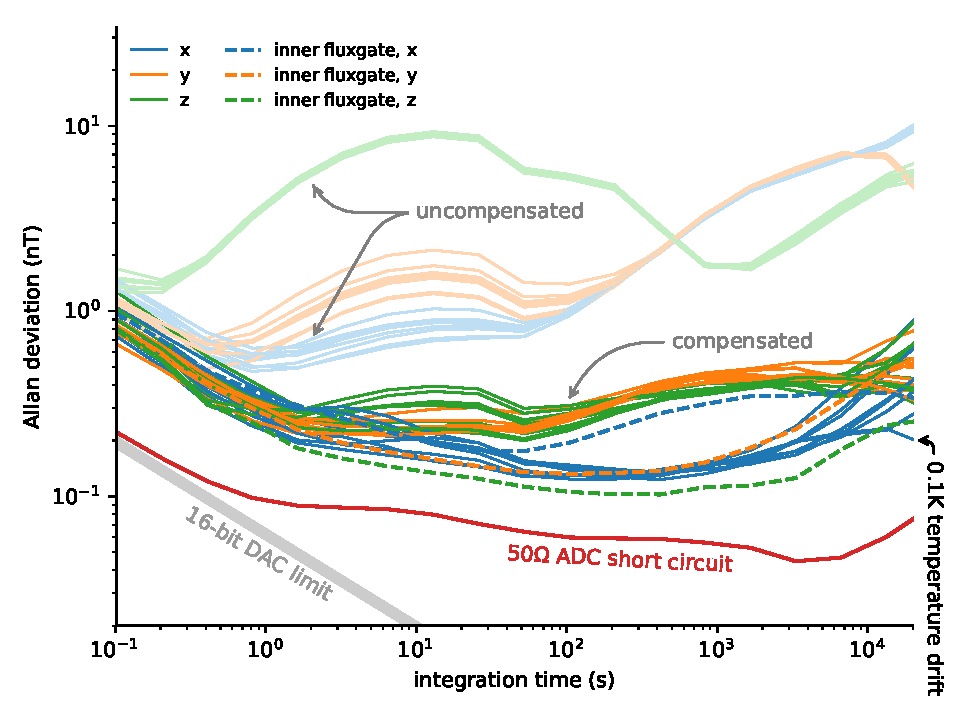
\includegraphics[width=\linewidth]{gfx/prototype/run8_field_stability.pdf}
  \caption{The stability of the active magnetic field compensation. The Allan deviation is plotted as the function of integration time. The three colours depict the three spatial directions. The uppermost three groups of thin, solid lines depict the uncompensated field $\mathbb{B}_0$ measured by the feedback sensors. In the dense group of lines below, around \SI{20}{\nano\tesla} (corresponding to a temperature stability of \SI{0.1}{\kelvin}, as specified for the fluxgates), are: the compensated field measured by the feedback sensors $\mathbb{B}$ (solid) and the compensated field measured by a non-feedback fluxgate in the centre of the system (dashed).
  % field measured inside a two layer $\upmu$-metal shield (dotted).
  Below that depicted are: the stability of the readout of a short-cut ADC channel (red) and the limit set by the quantisation noise of the 16-bit DACs (grey).}\label{fig:prototype_stability}
\end{figure}

To assess the stability, the system run during a night, with no known activity in the immediate surrounding of the laboratory. The registered Allan deviation is plotted in Fig.\,\ref{fig:prototype_stability}.
% The colour convention follows the one of Fig.\,\ref{fig:prototype_compensation_time}---the three spatial components are depicted with blue, orange and yellow and each line corresponds to one sensor.
The three uppermost groups of curves depict the stability of the uncompensated field $\mathbb{B}_0$ (as calculated with Eq.\,\ref{eq:uncompensated_field}). That the stability differed between the spatial components is not a concern---there is no reason to expect the disturbance to be anisotropic. Below, at around \SI{20}{\nano\tesla} over a wide range of integration time, is large group of curves. Among them are the thick, solid ones depicting the compensated field $\mathbb{B}$. Even in the most quiet of the conditions in the laboratory the system improved the stability of the field by a factor of two~($x$) to thirty~($z$).

In the previous section we indicated, that the case of high-order variations the field in the centre of the system was stabilised better then the one measured by the feedback sensors. In the plot the stability of the sensor in the centre is depicted with dashed lines. They lie in the large group around \SI{20}{\nano\tesla},
% although rather on its lower side,
suggesting that the variations during the measurement were homogeneous.

% Why was the improvement not better? In the plot there seems to be a fixed limit for the stability. Another set of curves, the dotted ones, provide a hint. They depict the stability of the field observed with an additional sensor mounted inside a two-layer $\upmu$-metal shield, which should provide a factor of a hundred in shielding (the second layer was a cylinder without end caps aligned with the $z$-axis of the sensor, hence the worse performance in this direction). Yet, the registered stability is no better than that of the active stabilisation system.

Why was the improvement not better? The limit came most likely from the temperature drifts. According to the specification of the Stefan Mayer Instruments FLC3--70 sensor it drifts \SI{2}{\nano\tesla\per\kelvin}, so the observed stability corresponds to temperature stability as small as \SI{0.1}{\kelvin}. Even at night the temperature in a not temperature-stabilised laboratory cannot be expected to be more stable that that. This limit can be pushed a factor twenty lower with higher-quality (and more expensive) sensors. Commercially available Stefan Mayer Instruments FL1--100 and Bartington Mag-03 are specified to drift \SI{0.1}{\nano\tesla\per\kelvin} with a $\SI{\pm 100}{\micro\tesla}$ measuring range.

However, below is another limitation. Figure\,\ref{fig:prototype_stability} features also a red line labeled ``\SI{50}{\ohm} ADC shortcut''. This is the stability of the readout of an ADC channel with the terminals connected with a \SI{50}{\ohm} resistor. Even if the magnetic field sensors would have output a perfectly stable voltage, the digitised information would be only this stable. A higher class digitisers could perform better.

Interestingly, the stability was fully defined by the measurement chain: the sensors and the digitisers. Instabilities of the output chain, DACs and amplifiers, indistinguishable from changes in the magnetic field, were corrected by the system itself. One exception is the discrete nature of the currents that can be applied. The lowest curve on the plot is the limit on the stability due to the bit depth of the DACs. A quantisation resolution $\Delta$ corresponds, on average, to a white noise with RMS amplitude $\Delta / \sqrt{12}$ (derived for example in Sec.\,IV.A in~\cite{Gray1998}). This noise scales then down as $\tau^{-1/2}$ with the integration time. The system's 16-bit DACs had $2^{16}$ levels mapped onto a $\SI{\pm 100}{\micro\tesla}$ range. This defines the quantisation at the feedback time of inverse $\SI{200}{\hertz}$. In total the limit from the quantisation at the integration time $\tau$ is:
\begin{equation}
  \frac{ \SI{200}{\micro\tesla} }{ 2^{16} \ \sqrt{12} \ \sqrt{ \SI{200}{\hertz}\ \tau}, . }
\end{equation}
Aside from the obvious---increasing the bit depth of the DACs---this limit can be pushed further by increasing the feedback frequency or decreasing the range of the operation.



% \note{Maybe a paragraph comparing this stability to the PSI system}
% It should be noted that at PSI the stability registered was \ldots more stable than the ETH laboratory. Better sensors

% \note{The process of winding a coil? Should be described!}


% \section{Testing the new feedback with the big system}
% Not sure where to put it, but somewhere in this chapter.

% Does not outperform, but is for example completely parameter-free (no I parameters), any field can be used as the target field.


\section{Open-design cage}
The disadvantage of the first-iteration design, pictured in Fig.\,\ref{fig:prototype_photo_inside}, was that the cage was fully closed, making putting anything inside, or taking outside, essentially impossible. In particular, one of the areas the active magnetic field compensation system prototype could be used to investigate is the effects of a $\upmu$-metal shield, which would need to be inserted into it.

% \note{Do I really find it necessary to describe the three possibilities that I considered?}

% Three designs with the inside accessible were considered.
% \marginpar{D-subminiature connectors with soldering contact were considered for this purpose. Two per edge.} The process of winding a coil would be much to much.
% In the first, connectors could be built in along edges of one of the faces (twenty, if the face is one of the small ones). To access the inside the connectors would have to be disconnected and then the face removed. The connectors would have to have as much as 30 pins, each connected to at least \SI{1}{\milli\meter} thick wire. The main disadvantage of this solution would have been considerable effort in terms of soldering.
% % Adding more coils would mean exchanging all connectors.
% The second design would feature a removable face without the need for connectors. The wires laid on one face would be separate from those on the rest of the structure. Along the edge where the face would be separated two cable channels would run in parallel next to each other, one belonging to the removable face. This would inevitably lead to some effective current cancellation along the edges of the removable face. \note{Explain why}.

% The third way was to design a system with out wires on one face at all. This solution had the immediate advantage of demonstrating the power of the coil design method. The next iteration is designed with one face (rectangular one, $Y-$) left open. Designed fully following the algorithm.

The solution was to modify a system in way, that on one of the faces there would be no wires at all. As neither the coil design method (Ch.\,\ref{ch:coil_design}) nor its implementation are restricted to regular grids, it could be fully realised within the framework. In the scope of this work coils corresponding to Cartesian harmonic polynomials $n = 1, \ldots, 8$ (Tab.\,\ref{tab:coils_cartesian_harmonics}) were designed and the $y$-coil ($n = 2$) was wound and mapped. The face that was left open is a square one, the one to the left in Fig.\,\ref{fig:prototype_photo}.

% This solution had the immediate advantage of demonstrating the power of the coil design method. The next iteration is designed with one face (rectangular one, $Y-$) left open. Designed fully following the algorithm.

\begin{figure}
  \centering
  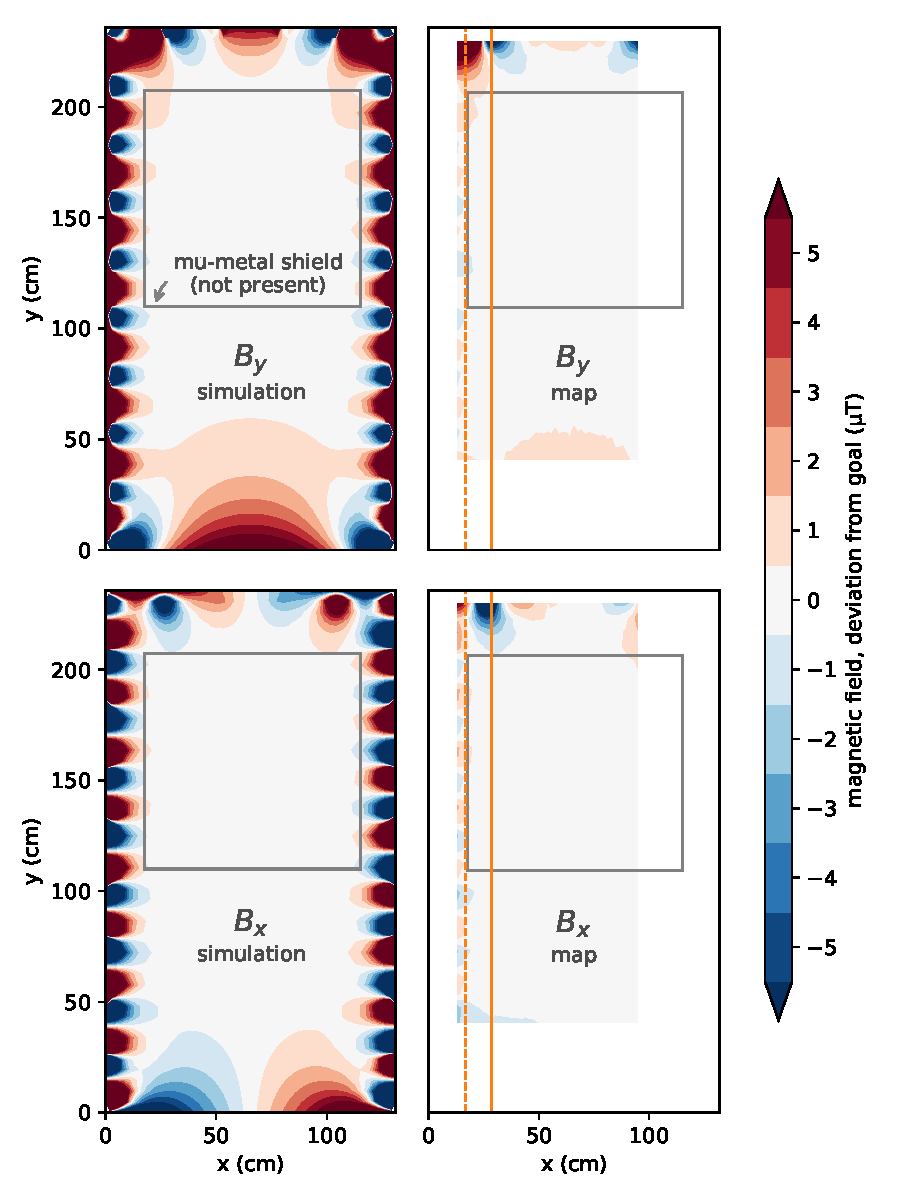
\includegraphics[width=\linewidth]{gfx/prototype/open_planar_map_comparison.pdf}
  % 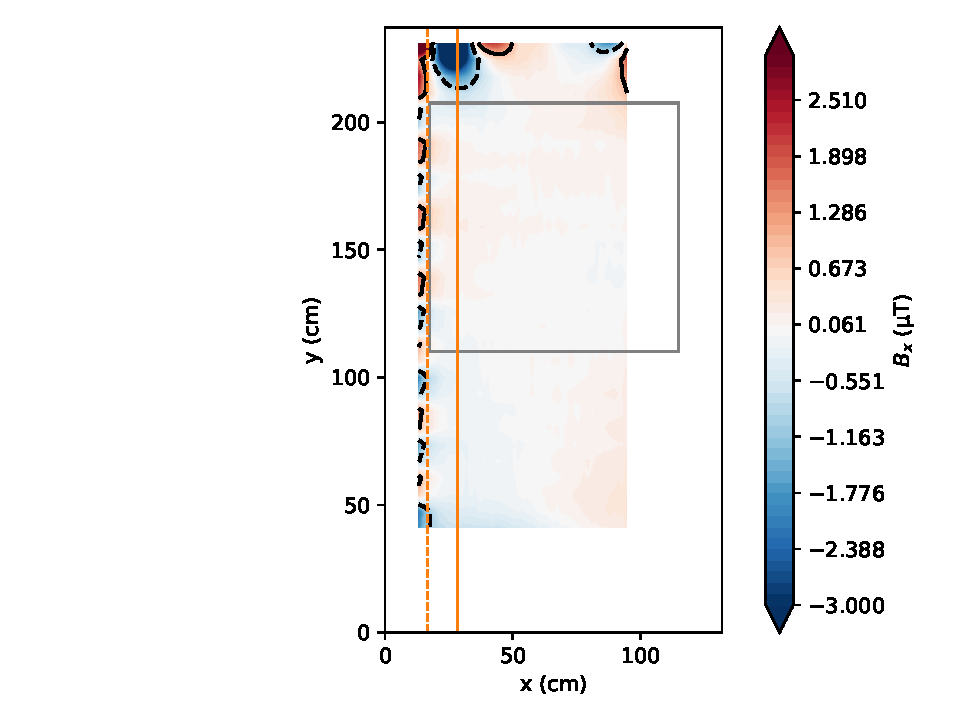
\includegraphics[width=0.45\linewidth,trim={5cm 0 0 0},clip]{gfx/prototype/open_planar_map_Y_Bx.pdf}\quad
  % 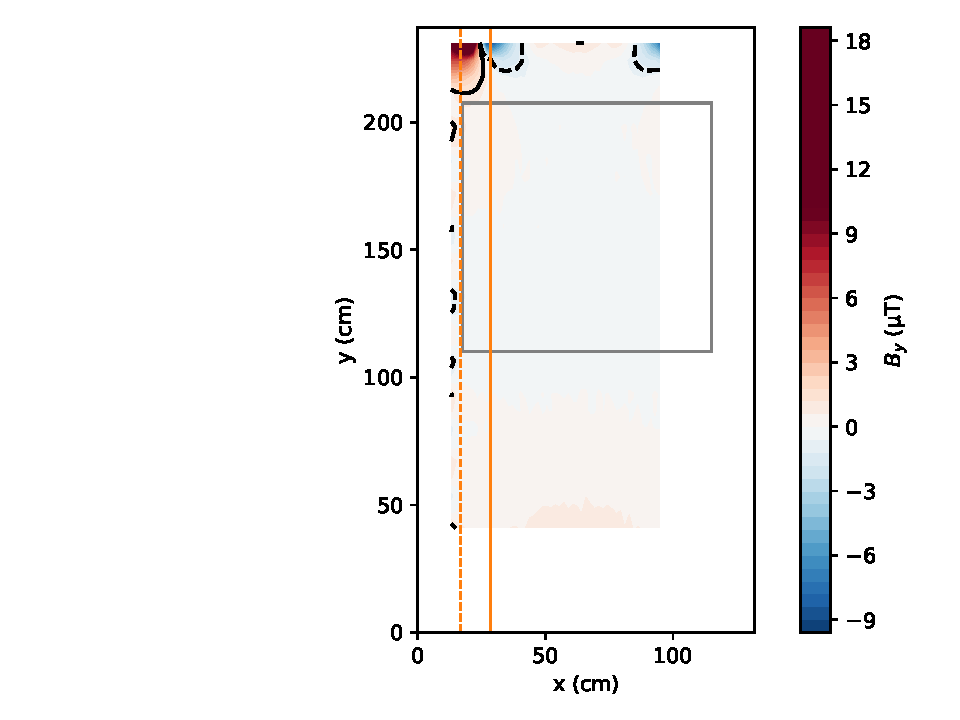
\includegraphics[width=0.45\linewidth,trim={5cm 0 0 0},clip]{gfx/prototype/open_planar_map_Y_By.pdf}
  \caption{The simulations (left column) and maps (right column) of the field of the $y$-coil. In the bottom row the $x$ component of the field is shown, in the top one: the $y$ component, the latter relative to the goal value of \SI{50}{\micro\tesla}. The contour of a $\upmu$-metal shield intended to be put in the system is depicted. To account for misalignments of the sensor the map has been normalised to the average field measured in the middle region of highest homogeneity. The mapped field along the vertical orange lines is plotted in Fig.\,\ref{fig:prototype_open_design_Ycoil_map_section}.}\label{fig:prototype_open_design_Ycoil_maps}
\end{figure}

\begin{figure}
  \centering
  \includegraphics[width=\linewidth]{gfx/prototype/open_planar_map_Y_By_section.pdf}
  \caption{The measured field of the $y$-coil along the solid and dashed lines depicted in Fig.\,\ref{fig:prototype_open_design_Ycoil_maps}. The thin, dashed lines depict the field \SI{16.6}{\centi\metre} away from the the surface of the coils in the $x$ direction (the fiducial volume was \SI{15.5}{\centi\metre} away). The thick, solid lines correspond to a distance of \SI{28.5}{\centi\metre}. The vertical line on the right depicts the surface of the coils along $y$.}\label{fig:prototype_open_design_Ycoil_map_section}
\end{figure}

In Fig.\,\ref{fig:prototype_open_design_Ycoil_maps} both simulations and maps of the field of the $y$ coil are shown.
\marginpar{In the whole fiducial volume the homogeneity was predicted to be stricly better than \SI[detect-all=true]{4}{\percent}.}
In the simulations the homogeneity was predicted to be \SI{2}{\percent} (\SI{1}{\micro\tesla} in the \SI{50}{\micro\tesla} field in the figure) in the $97.5 \times 97.5 \times \SI{97.5}{\centi\metre}$ volume (depicted in grey the figure) that would be occupied by a $\upmu$-metal cube intended to be put in the system. The measured field, mapped as described in Sec.\,\ref{sec:prototype_mapping}, confirms that the homogeneity could be achieved in practice. All three components of the field along the orange lines are detailed in Fig.\,\ref{fig:prototype_open_design_Ycoil_map_section}.

% The simulation of the field produced by the optimal design of the $y$-coil is presented in the upper part of Fig.\,\ref{fig:prototype_open_design_Ycoil_maps}. On the left-hand side the deviation of the $x$ component from zero is shown, on the right-hand side: one of the $y$ component from \SI{50}{\micro\tesla}. In the bottom of the figure a map of the two components is plotted. Additionally, two sections of the map, along the vertical lines depicted in orange, are presented in Fig.\,\ref{fig:prototype_open_design_Ycoil_map_section}. The dashed line is xxx away from the surface of the coils and corresponds to the edge of the fiducial volume. The design fully meets the specification of \SI{2}{\percent} homogeneity in the fiducial volume.

% and the map of the $y$-coil are presented in Fig.\,\ref{fig:prototype_open_design_Ycoil_maps}. In Fig.\,\ref{fig:prototype_open_design_Ycoil_map_section} the section along the $y$ direction is plotted.
% Now some thoughts about it. We see, that it behaves exactly as expected. For now the colours are inverted.

% \note{It is now a bit weird, that I have a detailed wiring plan for the $x$-coil, but I write more about the $y$-coil (the one I have)}.

\begin{figure}
  \centering
  \includegraphics[width=\linewidth]{gfx/prototype/open_design_Xcoil_field_XY_z0_33.png}
  \includegraphics[width=\linewidth]{gfx/prototype/open_design_n5coil_field_XY_z0_33.png}
  \caption{Simulation of the open-design cage. The colour represents the deviation from the target field, for the $x$, $y$ and $z$ components of the field. Section in the XY plane at height $z=\SI{33}{\centi\meter}$ is shown. The open face is on the bottom of the plots. Top: coil designed to produce a homogeneous field along $x$ (left-to-right on the plot). Bottom: $n=5$ gradient (see some table somewhere)\ldots}\label{fig:prototype_open_design_simulation}
\end{figure}

\begin{figure}
  \centering
  \includegraphics[width=\linewidth]{gfx/prototype/open_design_Xcoil_coils.pdf}
  \caption{The first 22 (out of 64) loops of the $x$-coil in the open-design cage. For each loop the the digits indicate the number of \SI{5}{\ampere}, \SI{1}{\ampere} and \SI{0.1}{\ampere} windings (per \SI{50}{\micro\tesla} field, leading zeros are omitted). A half of the cage is flattened out, the other being identical on symmetry grounds. The open face is located to the left. The faces have been coloured to help in orientation.}\label{fig:prototype_open_design_Xcoil_coils}
\end{figure}

The remaining seven coils of were designed. Winding them, however, was beyond the scope of this work.
The simulated field produced by the optimal designs for the $x$-coil and $n = 5$ (Tab.\,\ref{tab:coils_cartesian_harmonics}) are presented in Fig.\,\ref{fig:prototype_open_design_simulation}.
Despite lack of one face in the grid the field is reproduced in a volume large enough to fit the $\upmu$-metal cube, even in the case of the linear-gradient coil. In Fig.\,\ref{fig:prototype_open_design_Xcoil_coils} the first 22 (out of 64) loops of the $x$-coil are depicted.
Note in particular the high density of the cables along the edges of the open face.
% Except the part near the open face (at the bottom of the plots) the field in the volume is reproduced in the whole fiducial volume down to \SI{2}{\percent} (\SI{1}{\micro\tesla} on a \SI{50}{\micro\tesla} field), even for the gradient coil.
% Fig.\,\ref{fig:prototype_open_design_Xcoil_coils} shows the first 22 (out of 64) current loops of the $x$ coil.
%\note{All with 1A wires? not much more} The numbers show the number of windings in the 5A, 1A and 0.1A scheme.

% \note{Here I could mention how inhomogeneous was the field in the lab. I.e.\ how much field was still left when running the homogeneous compensation. This would motivate the need for the linear gradient coils.}

% The calculation with the fiducial volume of\ldots done for homogenous and 1st gradient coils. Fig.\,\ref{fig:prototype_open_design_simulation} presents the sections for\ldots Fig.\,\ref{fig:prototype_open_design_Xcoil_coils} shows the first 22 (out of 64) current loops. \note{All with 1A wires? not much more} The numbers show the number of windings in the 5A, 1A and 0.1A scheme.

The open-design $y$-coil was a significant step forward in comparison to the closed-cage design. It has been demonstrated, that the coil design framework is capable of handling irregular grids, and the designs can be successfully realised in practice. While the prototype at ETH could be further extended by winding the remaining seven coils, the positive results of the $y$-coil can already support the case for designing a system for the n2EDM experiment.



\section{n2EDM design}
Let us recall the discussion in Sec.\,\ref{sec:n2EDM_challenges} on the design challenges of an active magnetic field compensation system for the n2EDM experiment. The main point of concern were the spatial constraints. Firstly, there would not be much space available around the $\upmu$-metal shield, calling for a coil system with a large fiducial volume. Secondly, a cage that would avoid collisions with other components of the experiment and facilities in the hall the would need to be irregular.

\begin{figure}
  \centering
  \includegraphics[width=\linewidth]{gfx/prototype/n2EDM_system_top.png}
  \caption{Replace with a better figure showing the design\ldots The best show the front face, too.}\label{fig:n2EDM_design_top}
\end{figure}

A cage for the compensation coils was incorporated in an existing CAD model of the experiment. It was composed out of rectangles maximally around \SI{1.5}{\metre} large. Care has been taken to avoid conflicts with other parts of the apparatus.
The cage, depicted in Fig.\,\ref{fig:n2EDM_design_top}, was then implemented in the coil-design framework.

\begin{figure}
  \centering
  \includegraphics[width=\linewidth]{gfx/prototype/n2EDM_field_Xcoil_XY_z6_4.png}
  \includegraphics[width=\linewidth]{gfx/prototype/n2EDM_field_n6coil_XY_z6_4.png}
  \caption{Simulation of the n2EDM design. The colour represents the deviation from the target field, for the $x$, $y$ and $z$ components of the field. Section in the XY plane at height $z=\SI{6.4}{\meter}$ is shown. The open face is on the bottom of the plots. Top: coil designed to produce a homogeneous field along $x$ (left-to-right on the plot). Bottom: $n=6$ gradient (see some table somewhere)\ldots}\label{fig:n2EDM_design_fields}
\end{figure}

\begin{figure}
  \centering
  \includegraphics[width=0.9\linewidth]{gfx/prototype/n2EDM_coils_field.pdf}
  \caption{The quality of the field produced by the coils designed for the n2EDM experiment, quantified by the histogram of the deviation of the design's simulated field from the target one, as measured on the surface of the $\upmu$-metal shield. One entry is a difference in one spatial direction. The designs for the homogeneous coils, similar to one another, have been averaged. The ones for the linear gradients were as well.}\label{fig:n2EDM_design_deviation}
\end{figure}

A set of coils has been designed for the first eight Cartesian harmonics (Tab.\,\ref{tab:coils_cartesian_harmonics}). The field simulated for an $x$-coil and a $n = 6$ linear gradient are depicted in Fig.\,\ref{fig:n2EDM_design_fields}, with the contour of the $\upmu$-metal shield depicted in grey. \note{Still need to mark the shield contour there}. The quality of the field, as simulated on the surface of the $\upmu$-metal shield, is plotted in Fig.\,\ref{fig:n2EDM_design_deviation}. The deviation from the pure harmonics is shown for roughly the fields expected to be in the experimental site. \note{Need to refer to the mapping campaign here, blocked by Solange at the moment.} When compensating a perfectly homogeneous \SI{50}{\micro\tesla} field, the remnant is expected to be $< \SI{1}{\micro\tesla}$ (which corresponds to \SI{2}{\percent}). In the case of a \SI{20}{\micro\tesla\per\meter} linear gradient it would be $< \SI{6}{\micro\tesla}$ (\SI{6}{\percent} for the \SI{5}{\metre} large shield).

\note{A paragraph linking all that to mapping---what kind of fields will we expect? Need to talk to Klaus to clarify, what I can put in my thesis and what should I leave for Solange.}



\section{Conclusion}
What is new about the next-generation active magnetic field compensation?
Predefined grid, can deal with spatial constrained. Shared between different coils - can built many ones. In particular, it is possible to construct coils for the mutually orthogonal terms of the Cartesian harmonic expansion of the field. This simplifies the control of the system, by making it well defined, there is no need for regularisation.

What have I done, how successful was it?
A laboratory-sized prototype has been constructed on a closed, regular grid. feasibility of building. The practical advantages of using cable channels as the support structure for the coils. Working stabilisation has been demonstrated for homogeneous fields.
In the second iteration, one face of the grid was left open, making the coils designs significantly more complex. A coil for one homogeneous component has been wound and characterised.

It can find specially when the volume is large and the spatial constraints are tight. Should I mention G-bar experiment, for example?

What is it good for and what is the outlook?



% The fields stays within \SI{1}{\percent} of the target in the fiducial volume for the homogeneous coils.
% Around 80 loops for each of the homogeneous coils.

% Important question: how well is the field reproduced in the volume occupied by the shield?


% Repeat a bit what it was about.

% Maybe present some coils, too! Why not, but time-consuming.




% The volume is cubic.

% The SFC system is going to be very large --- $\unit[6x6x6]{m^3}$. Elaborate designs, such as wires of variable length, or arbitrarily bended wires would be complicated to realise in such scale.

% Moreover, the system is going to enclose the whole apparatus.
% Super crucial --- many coils on the same surface 3 for the first order compensation, but then 9 for gradients. That is already 12 coils. If one only restrict oneself to a surface, it is guaranteed to end up with it densely covered with wires. In this approach the geometry is limited by design.

% Mention, that the \micro-metal presence does not disturb much, as it is already placed in a small field.


% Design goals / challenges:
% \begin{enumerate}
%   \item Better shielding factor. Attenuation by a factor of 50 in the whole volume of the shield. The design goal has been set to reach at most 2\% of the ambient magnetic field in the
%   whole volume of the experiment. In \SI{50}{\micro\tesla} this corresponds to a nice value of \SI{1}{\micro\tesla}.
%   \item Very large fiducial volume --- due to spatial constrains of the experimental site --- biological shielding. PUT IMAGE!!! Not only is the compensation expected to be better, but also provide a much larger volume. Next version of the experiment --- much larger.
%   \item As is nEDM --- many coil system. But orthogonal, or at least close to one. Three coils for compensating the three homogeneous components of the magnetic field. Then 9 for gradients. The strongest fields are low-order, and only these require strong compensation coils (thick wires, big and expensive power supplies). The higher-order coils may be constructed with thinner wires and cheaper power supplies.
%   Additionally, this makes the control of the system simpler.
%   This also states the problem better. One has to design and construct coils that create homogeneous field in the volume occupied by the shield. Maybe elaborate more on the field decomposition!
%   \item Coil tailored for the specific magnetic environment of the n2EDM site. Coils tailored for nearby magnets.
% \end{enumerate}

\chapter{Mapping}
A mapping campaign is planned in the experimental hall, where the n2EDM experiment is going to be located. There are numerous magnetic sources in the vicinity of the site, causing the magnetic environment to be unusually complex. Taking a number of magnetic field maps will provide knowledge necessary to make sure, that the n2EDM compensation system will be able to cope with the environment. A 2.5m high mobile tower with 10 3-axis magnetic field sensors has been constructed. The position and orientation of the tower is measured with cable extension transducers, which makes the mapping process as simple as sweeping an area with the tower. Reproducibility of the maps measured with the device was proven to be better than \SI{0.5}{\micro\tesla}.


\section{The idea}
The precision is not crucial, but the time it takes to measure a map is. The shorter it takes to make a map, the less it is influenced by external conditions. It cannot always be mapped during ,,quiet periods''. We want to have maps of magnetic fields that occur only during busy day-times. For example the crane, or SULTAN or other magnets.

For these reasons it has been decided, that the mapping would consist of a tower. The tower would be moved manually (don't use the future tense here), the position and orientation measured along the magnetic field. Then describe the setup here, briefely. The scalar information is enough to localise sources of magnetic field.

Vector information is useful if the data are to be used for example to calculate dedicated compensation coils for some sources of disturbance.

The setup is shown\ldots The mapper was a tower this and that high, with ten fluxgate magnetometers mounted on it.
The three analogue string potentiometers were mounted on a rigid L-piece. The base element is the string potentiometer. It consists of a wire wound on a spring-loaded spool, the spool attached to a potentiometer. For maximal linearity it is constructed in a way, that the string is wound one in layer only. The string string potentiometers give an analogue signal proportional to the extension of the wire. This information was used to determine the position and orientation of the tower.
\marginpar{Other names for a string potentiometers include: cable-extension transducer, draw-wire sensor and string pot.}
\mnote{The terms like the tower need to be clear by here.}


Let us start with a two-dimensional problem. Span two strings between a magnetic field sensor, each to a fixed position in the room. Based on trilateration. With two strings there are two solutions, but we are always able to detect the correct one.

To get the vector information about the field, also the orientation of the sensors needs to be known. For that an arm can attached to the sensor and a third string spanned to the arm's end.

Now is the time for the nice drawing of the geometry solution.



\section{Principle of a string-potentiometer--based mapper}
For a given signal of a calibrated string potentiometer the points where the free end of the string can be make up a circle. The centre at the location of the body of the sensor, the radius equal to the extension of the wire. In the mapper setup there are two string potentiometers mounted on the fixed L-piece, both extended to a single point on the tower. This points lies on the intersection of the two circles. The problem of determining the location based on the measurement of the distances to a set of fixed points is called \emph{trilateration}.

\marginpar{Other position determination methods include triangulation (measurement of angles between lines connecting a set of fixed points) and multilateration (measurement of the differences of distances between a set of fixed points).}

\begin{figure}
  \centering
  \includegraphics[width=0.9\linewidth]{gfx/mapping/geometry.png}
  \caption{\ldots}
  \label{fig:mapping_geometry}
\end{figure}

The geometry is presented in Fig.\,\ref{fig:mapping_geometry}.The two string potentiometers used to determine the position are located is points $(x, y) = (0, y_0)$ and $(x_0, 0)$ (in the L-piece coordinate system, orange in the figure).
The tower, here point-like, is at $(x,y)$.
The wire extensions are $r$ and $\rho$. For the sake of simplicity, we first give the solution in the coordinate system depicted in green \note{maybe use the A B and C names here already}, where the first string potentiometer is in $(0,0)$ and the second in $(d, 0)$ (with $d = \sqrt{x_0^2 + y_0^2}$). In this coordinate system the tower is in $(\xi, \nu)$. From simple geometry the solution for the position of the tower is:
\begin{align}
  \xi & = \frac{1}{2d} \left( d^2 - \rho^2 + r^2 \right) \\
  \nu & = \frac{1}{2d} \sqrt{ (-d + \rho - r) (-d - \rho + r) (-d + \rho + r) (d + \rho + r) }
\end{align}
The transformation to the L-piece, orange, coordinate system is rotation by the angle $\alpha = \mathrm{ctan} \frac{y_0}{x_0}$ followed by a translation:
\begin{equation}
  \begin{pmatrix}
    x \\
    y
  \end{pmatrix}
  =
  \begin{pmatrix}
    \cos \alpha & -\sin \alpha \\
    \sin \alpha & \cos \alpha
  \end{pmatrix}
  \begin{pmatrix}
    \xi \\
    \nu
  \end{pmatrix}
  +
  \begin{pmatrix}
    0 \\
    y_0
  \end{pmatrix}
\end{equation}

\note{Give here a general formula for an intersection of two circles. Need to check the LabVIEW code?}

With two circles there are two solutions, symmetric around the line connecting the centres of the circles. However, during the mapping the tower stays in the area inside the positive quarter of the L-piece coordinate system.
We assume never to be in the small triangle to the left and down from the line connecting the two string potentiometers.

The problem of determining the orientation of the tower is, in fact, the same as the one of the position. The setup includes a third string potentiometer, with the string attached to \note{there are two $d$s in the picture!} an arm of the tower (depicted in violet in Fig.\,\ref{fig:mapping_geometry}) of the length $a$. The end of the arm lies on the intersection of two circles: the one centred in the centre of the tower and radius $a$, and the one centred at the sensor end of the third potentiometer with the length equal to the wire extension.



\section{LPSC campaign}
First the setting. Magnetic characterisation of a new laboratory room, designated for Hg-199 magnetometry research.
A picture of the room (and the mapper, too?).

The setup is shown\ldots The mapper was a tower this and that high, with ten fluxgate magnetometers mounted on it.
The three analogue string potentiometers were mounted on a rigid L-piece (give the positions).
\marginpar{A string potentiometer has a spring-loaded spool attached to a potentiometer. For maximal linearity it is constructed in a way, that the string is wound one layer only.}
\marginpar{Technical details of the setup: fluxgate -- Stefan-Mayer FLC3-70, readout frequency -- xxx, ADC -- aoethu, string potentiometers -- Micro-Eplison xxx}

Then about the reproducibility.

The subject of this report is a mapping of the magnetic field performed in Laboratoire de Physique Subatomique & Cosmologie (LPSC) in Grenoble, France in the days 6.-10.03.2017 by Michał Rawlik, with the much appreciated help of Rémi Faure, Guillaume Pignol and Dominique Rebreyend.

The goal was to map two rooms, Bastille and Chalet, considered to host a test setup for Hg-199 magnetometry. The setup is sensitive to ambient magnetic fields. In particular, gradients above roughly 10 nT/cm cause an increase in the depolarisation rate of the mercury atoms.

To map the field a device called simply the mapper was used, described below.

This report is bundled with photographs documenting the measurement process, the datafiles taken and plots produced in the analysis. All the analysis code is part of this report. The report is a jupyter notebook using python3 code.


The picture above shows the two main parts of the mapper. The first is the movable tower equipped with 10 3-axis Stefan Mayer FLC3-70 fluxgates. The second is the stationary coordinate sytem onto which three WDS-15000-P115-SA-P string extension transducers (also called string pots) are attached. The string pots are equipped with a custom made attachments that allow the string to come at an angle out of the device. The strings are attached to the tower, two to a point where the vertical beam with fluxgates are, one to one of the arms with wheels. This allows for determination of both position and orientation of the tower.

The data acquisition system is located on a cart. It consists of a power supply used to put a constant current through the string potentiometers, custom-built crate for the fluxgates, which supplies them with power and conditions the incoming signals, and a National Instruments PXI crate, reading the analogue voltage signals from the fluxgates and the stringpots. The digitisation of all signals is simultaneous.

The picture below shows a panoramic view of the room.

The coordinate system is visible in the lower-left corner. To the right are the entrance door, in the middle a power outlet box is visible. Behind the wall with the power outlet box there is a pump, which has been at some point removed. The room is a wooden structure built in a hall. The hall is made of steel beams and sheets. The room's wall with the power outlet is located close, less than 1 metre, to the steel wall of the hall. The hall features a gantry crane, several metres above the roof of the room. On the roof of the room there are air conditioning devices, standing about a metre above the roof on steel legs. The legs have rather large feet, possibly with a steel plate inside.



\section{PSI campaign}

Acknowledge that it is a joint work with Solange Emmenegger.

Describe the changes to the setup: now the geometry is like this and this. Need probably a detailed picture of the geometry of the setup and the mapper.

About the method to fit the calibration parameters to the fixed points.

% -------------------------------------------------------
% AXION SEARCH
% -------------------------------------------------------
\ctparttext{Most of the universe's matter content, an estimated \SI{84}{\percent}, is dark matter.
Among the candidates for its constituents is an ultra-low-mass axion.
In this part a search for a signature of an axion dark matter in the data of the nEDM experiment at PSI is described.
The ratio of the spin-precession frequencies of stored ultracold neutrons and ${}^{199}$Hg atoms was analysed for an axion-induced oscillating electric dipole moment of the neutron and an axion-wind spin-precession effect.
No signal consistent with dark matter was observed for the axion mass range $\SI{e-24}{\electronvolt} \leq m_a \leq \SI{e-17}{\electronvolt}$.
The null result set the first laboratory constraints on the coupling of axion dark matter to gluons, which improved on astrophysical limits by up to three orders of magnitude.
It also improved on previous laboratory constraints on the axion coupling to nucleons by up to a factor of 40.

The first section in this part introduces the subject of axion-like dark matter.
In the second the method of choice for the analysis, the least-squares periodogram, is discussed.
The methodology developed there is then applied to the PSI nEDM dataset in the third section.
The part concludes with a proposal for a resonant search for an oscillating electric dipole moment.}
\part{Axion-Dark-Matter Search}
% \chapter{Axion--Like Particles search with ultracold neutrons}
%
% \label{ch:axions}

\chapter{Introduction}
\label{ch:axions-intro}





% \section{Motivation}
% \begin{figure}
%   \centering
%   \includegraphics[width=0.5\linewidth]{gfx/axions/Standard_Model_of_Elementary_Particles.pdf}
%   \caption{Standard Model particles - known matter.}
%   \label{fig:axions_SM_particles}
% \end{figure}
% The twentieth century is a success story of the Standard Model of Particle Physics, whtested in laboratories with extraordinary precision \note{cite something cool}.

% ost of them falling into two categories: Weakly Interacting Massive Particles (WIMPs) and axions. Axions, in contrast to WIMPs, would be very light, but abundant. And could be 

% As early as 1884 Lord Kelvin has estimated the number of bodies in our Milky Way galaxy based on the velocity distribution and noted that most of them we do not see. \note{cite}

% Over the next hundred years this approach, pioneered by Zwicky (ref) has been extended. Measuring the \emph{rotation curves} of the galaxies, the relation between the velocity of the stars in their motion around the galactic centre and the distance from it, provided a way to estimate the distribution of the mass. Gravitational lensing is another method.

% It is the fundamental curiosity that drives the desire to understand what is Dark Matter made of.

% Axions and WIMP are searched for with fundamentally different techniques. WIMP detectors, like XENON (ref) try to detect a single interaction signature of a WIMP particle with the mass of the detector. The detectors are massive, many tons, and almost background-free. In attempts to detect axions one looks for very weak signals coming from the omnipresent bulk axion matter.

% We will focus on axions.


% This part is concerned with a search for a signature of an axion dark matter in the data measured by the nEDM experiment at PSI\@. The signature would be an oscillation in the array of the measured ratios of the precession frequencies of the neutrons and ${}^{199}$Hg atoms, as measured during normal nEDM data taking.

% The method of choice to quantify oscillations in the unevenly sampled array is the least-squares periodogram~\cite{Scargle1982}. In the next chapters we introduce the periodogram, discuss its properties and develop statistical methods for an oscillation search.

% % Then, the analysis itself is presented. 

% % methodology is developed, then the data.

% Here say, that we first develop the methods on a simple example in the next chapter. A search for an oscillating nEDM~\ref{eq:nEDM_axion} is presented.

% Then the next chapter is\ldots


% \section{Theoretical background}
\marginpar{This section is largely based on Ref.\,\cite{PhysRevX.7.041034}.}
Based on astrophysical and cosmological observations an estimated \SI{26}{\percent} of the total energy density of the Universe and \SI{84}{\percent} of its mass content is dark matter (DM)~\cite{Planck2015}. The observations give hints about the amount and distribution of DM, for example via rotational curves or gravitational lensing~\cite{ApJ1990}, but the micro-scale properties of DM, in particular its constituents, remain unknown.

Among the candidates for DM is an axion, a new scalar particle, initially proposed to solve the strong QCD problem (the strong sector in the Standard Model appears to be fine-tuned to be $CP$-even)~\cite{PhysRevLett.38.1440,PQ1977B,Weinberg1978,Wilczek1978,Kim1979,Zakharov1980,Zhitnitsky1980B,Srednicki1981}. 
It has been later generalised to axion-like particles, or simply axions~\cite{Witten1984,Conlon2006,Witten2006,Arvanitaki2010,Arias2012,Marsh2015Review}. Light ($m_a \lesssim \SI[per-mode=symbol]{0.1}{\electronvolt\per\clight\squared}$) axions can be produced efficiently via non-thermal production mechanisms, such as vacuum misalignment in the early Universe~\cite{Preskill1983cosmo,Sikivie1983cosmo,Dine1983cosmo}. They fill the universe as almost stationary particles and through gravity participate in the galaxy formation. As they fall, they gain speed ($\approx \SI[per-mode=symbol]{300}{\kilo\metre\per\second}$) and, as bosons, condensate into a coherent oscillating field ($\Delta\omega / \omega \sim \num{e-6}$)~\cite{Marsh2015Review}, with he frequency of the oscillation is set by the mass of the axion $m_a$:
\begin{equation}
  a = a_0 \, \cos\left(\frac{ m_a c^2 }{\hbar} \ t\right) \ .
\end{equation}

Due to its effects on structure formation~\cite{Khlopov1985}, ultra-low-mass axion DM in the mass range $\SI{e-24}{\electronvolt} \lesssim m_a \lesssim \SI{e-20}{eV}$ has been proposed as a DM candidate that is observationally distinct from, and possibly favourable to, archetypal cold DM~\cite{Hu2000,Marsh2014,Schive2014,Marsh2015Review,Hui2017}.
The requirement that the axion de Broglie wavelength does not exceed the DM size of the smallest dwarf galaxies and consistency with observed structure formation~\cite{Marsh2015B,Schive2015,Marsh2017} give the lower axion mass bound $m_a \gtrsim \SI{e-22}{eV}$, if axions comprise all of the DM\@. However, axions with smaller masses can still constitute a sub-dominant fraction of DM~\cite{Hlozek15}.

It is reasonable to expect that axions interact non-gravitationally with standard-model particles.
Direct searches for axions have thus far focused mainly on their coupling to the photon (see the review~\cite{Axion-Review2015} and references therein).
\marginpar{Axions are hoped to convert into photons in a strong magnetic field. Helioscopes look for energetic axions produced in the sun. Haloscopes are sensitive to a relict axion dark matter.}
% **WHY WAS THIS HERE?  (MALCOLM)** coherently oscillating spin-dependent effects due to the
%\note{BL: We should cite: The here described experiment obtained a new limit on axion-like particles using ultracold neutrons \cite{Afach2015Exotic}.}
%\note{YS: In the earlier (long) version of this paper, we actually had a reference to this paper and several other papers on related applications of ultracold neutrons to look for new physics. In the process of shortening the paper, the paragraph containing these references was cut out, but perhaps we could restore the references somewhere in the paper.}
Recently, however, it has been proposed to search for the interactions of the coherently oscillating axion DM field with gluons and fermions, which can induce oscillating electric dipole moments (EDMs) of nucleons~\cite{Graham2011} and atoms~\cite{Stadnik2014A,Roberts2014A,Roberts2014B}, and anomalous spin-precession effects~\cite{Flambaum2013Patras,Stadnik2014A,Graham2013}.
The frequency of these oscillating effects is dictated by the axion mass, and more importantly, these effects scale linearly in a small interaction constant~\cite{Graham2011,Stadnik2014A,Roberts2014A,Roberts2014B,Flambaum2013Patras,Graham2013}, whereas in previous axion searches, the sought effects scaled quadratically or quartically in the interaction constant~\cite{Axion-Review2015}.

In this part two axion couplings are considered: the one to gluons and the one to nucleons:
\begin{align}
\label{Axion_couplings}
\mathcal{L}_{\textrm{int}} = \frac{C_G}{f_a} \frac{g^2}{32\pi^2} a G^{b}_{\mu \nu} \tilde{G}^{b \mu \nu}  - \frac{C_N}{2f_a} \partial_\mu a ~ \bar{N} \gamma^\mu \gamma^5 N \, ,
\end{align}
where $G$ and $\tilde{G}$ are the gluonic field tensor and its dual, $b=1,2,\ldots,8$ is the  color index, $g^2 / 4 \pi$ is the color coupling constant, {\color{black}$N$ and $\bar{N} = N^\dagger \gamma^0$ are the nucleon field and its Dirac adjoint,} $f_a$ is the axion decay constant, and $C_G$ and {\color{black}$C_N$} are model-dependent dimensionless parameters.
Astrophysical constraints on the axion-gluon coupling come from Big Bang nucleosynthesis~\cite{Blum2014,StadnikThesis,Stadnik2015D}:~$m_a^{1/4} f_a / C_G \gtrsim 10^{10}~\textrm{GeV}^{5/4}$ for $m_a \ll \SI{e-16}{eV}$ and $m_a f_a / C_G \gtrsim \SI{e-9}{GeV^2}$ for $m_a \gg \SI{e-16}{eV}$, assuming that axions saturate the present-day DM energy density,
and from supernova energy-loss bounds~\cite{Graham2013,Raffelt1990Review}:~$f_a / C_G \gtrsim \SI{e6}{GeV}$ for $m_a \lesssim 3 \times \SI{e7}{eV}$.
{\color{black}Astrophysical constraints on the axion-nucleon coupling come from supernova energy-loss bounds~\cite{Raffelt1990Review,Raffelt2008LNP}:~$f_a / C_N \gtrsim \SI{e9}{GeV}$ for $m_a \lesssim 3 \times \SI{e7}{eV}$, while existing laboratory constraints come from magnetometry searches for new spin-dependent forces mediated by axion exchange~\cite{Romalis2009_NF}:~$f_a / C_N \gtrsim 1 \times \SI{e4}{GeV}$ for $m_a \lesssim \SI{e-7}{eV}$. }

The axion-gluon coupling in Eq.\,\ref{Axion_couplings} induces the following oscillating EDM of the neutron via a chirally-enhanced 1-loop process~%\footnote{Interaction (\ref{Axion_couplings}) also non-perturbatively induces a mass $m_a \approx 6C_G\,\mu\text{eV} \cdot (10^{12}\text{ GeV}/f_a)$.
%Axions with masses much smaller than this are theoretically fine-tuned.}
\cite{tuningfootnote,Witten1979,Witten1979B,Pospelov1999}:
%\note{KK: merge to [42-44]}
\begin{equation}
\label{eq:nEDM_axion}
d_\mathrm{n}(t) \approx +2.4 \times 10^{-16} ~ \frac{C_G a_0}{f_a} \cos(m_a t) ~ \si{\elementarycharge\centi\metre} \, .
\end{equation}
The axion-gluon coupling also induces oscillating EDMs of atoms via the 1-loop-level oscillating nucleon EDMs and tree-level oscillating P,~T-violating intra-nuclear forces (which give the dominant contribution)~\cite{Stadnik2014A,Flambaum1984EDM,Flambaum1984EDMB}.
In the case of $^{199}$Hg, the oscillating atomic EDM is~\cite{Stadnik2014A,StadnikThesis,Flambaum1985EDM,Flambaum1985EDMB,Flambaum2002EDM,Dmitriev2003A,Dmitriev2003B,Dmitriev2005,Engel2005,Engel2010}
\begin{equation}
\label{199Hg-EDM_axion}
d_{\textrm{Hg}}(t) \approx +1.3 \times 10^{-19} ~ \frac{C_G a_0}{f_a} \cos(m_a t) ~ \si{\elementarycharge\centi\metre} \, ,
\end{equation}
which is suppressed compared to the value for a free neutron (Eq.\,\ref{eq:nEDM_axion}), as a consequence of the Schiff screening theorem for neutral atoms~\cite{Schiff1963}.
%\note{KK: a question to our theory friends: Eqns. (2) and (3) suggest that $d_n$ and $d_\textrm{Hg}$ would have the same sign. Is this intended or are we rather talking about the modulus?}
%\note{YS: Yes, the same signs for $d_n$ and $d_\textrm{Hg}$ are intended here.}
%\note{MR: Should we explicitly point that out then?}
%\note{YS: I think this would be a good idea. We could explicitly add "+" signs in both Eqs. (2) and (3) to remove any ambiguity.}
%\note{CG: Might be good to comment that the Hg contribution is quite safely assumed to be negligible compared to the neutron for the purposes of this paper.}
The amplitude of the axion DM field, $a_0$, is fixed by the relation $\rho_a \approx m_a^2 a_0^2 /2$.
In this work is it assumed that axions saturate the local cold DM energy density $\rho_{\mathrm{DM}}^{\mathrm{local}} \approx \SI[per-mode=symbol]{0.4}{\giga\electronvolt\per\centi\metre\cubed}$~\cite{Catena2010}.




%Crucially, the constant amplitude of the axion DM field, $a_0$, is fixed by the known DM density at the location of the Earth, $\rho_{\mathrm{DM}}=\approx 0.4~\textrm{GeV/cm}^3$ \cite{Catena2010} (when reporting constraints on the couplings we assume axions make up all the local DM).


% Our experiment is also sensitive to the time-dependent energy shifts induced by the derivative coupling of an oscillating galactic axion DM field, $a = a_0 \cos(m_a t - \vtr{p}_a \cdot \vtr{r})$, with spin-polarised nucleons in (\ref{Axion_couplings}):
The derivative coupling of an oscillating galactic axion DM field, $a = a_0 \cos(m_a t - \vtr{p}_a \cdot \vtr{r})$, with spin-polarized nucleons in (\ref{Axion_couplings}) induces time-dependent energy shifts according to:
\begin{equation}
\label{potential_axion-wind}
H_{\textrm{int}} (t) = \frac{C_N a_0}{2 f_a} \sin(m_a t) ~ \vtr{\sigma}_N \cdot \vtr{p}_a \, .
\end{equation}
The term $\vtr{\sigma}_N \cdot \vtr{p}_a$ is conveniently expressed by transforming to a non-rotating celestial coordinate system (see, e.g.,~\cite{Kostelecky1999}):
\begin{align}
\label{sigma-p_a_2}
\vtr{\sigma}_N \cdot \vtr{p}_a  &= \hat{m}_F f(\sigma_N) m_a |\vtr{v}_a|  \notag \\
& \times \left[\cos(\chi) \sin(\delta) + \sin(\chi) \cos(\delta) \cos(\Omega_{\textrm{sid}} t - \eta) \right] \, ,
\end{align}
where $\chi$ is the angle between Earth's axis of rotation and the spin quantization axis ($\chi = \ang{42.5}$ at the location of the PSI), $\delta \approx - \ang{48}$ and $\eta \approx \ang{138}$ are the declination and right ascension of the galactic axion DM flux relative to the Solar System~\cite{NASA2014web}, $\Omega_{\textrm{sid}} \approx \SI{7.29e-5}{\per\second}$ is the daily sidereal angular frequency, $\hat{m}_F = m_F / F$ is the normalized projection of the total angular momentum onto the quantization axis, and $f(\sigma_N) = +1$ for the free neutron, while $f(\sigma_N) = -1/3$ for the $^{199}$Hg atom in the Schmidt (single-particle) model.

The scalar axion-gluon coupling and the vector axion-nucleon coupling would induce harmonic oscillations in the measurements of the nEDM experiment at PSI\@. In the scope of this analysis the time series of the ratio of precession frequencies of polarised neutrons and ${}^{199}$Hg atoms was tested for statistically significant oscillations. In the next chapter the methodology for this quantitative search is introduced.



% A transition paragraph about why we need a method to look in the frequency space and need to calculate the periodograms.
\chapter{Periodograms}
\label{ch:axions-periodograms}
The space of possible axion-induced signals is spanned by their amplitude (the strength of the coupling) and their frequency (the axion mass). The problem is, therefore, naturally set in the frequency domain. The analysis was performed in two steps. First, the measurements were transformed from the time domain into the frequency one by evaluating the periodogram of the time series. In the second step the periodogram was checked for statistically significant signals.

In this chapter we introduce the statistical methods used in the analysis. We start by defining the periodogram, which serves as a transition from time to the frequency space, natural for looking for oscillations. Next, we proceed to discuss the statistical properties of the periodogram.

% For the sake of pedagogy we will discuss the methodology on a simple example.



\section{Definition of the periodogram}
A \emph{periodogram} is an estimator of the power spectrum. It has been proposed as the preferred way to treat periodic signals as early as 1898~\cite{Schuster1898}. In its simplest form it is the squared magnitude of the discrete Fourier transform, which, however, is only possible for evenly sampled series. Lomb and Scargle have independently described a method to construct a statistically well-behaving periodogram for non-uniformly sampled data with unequal error-bars: the Least Squares Spectral Analysis (LSSA)~\cite{Scargle1982}. It is also known as the Lomb-Scargle periodogram.

% Many packages readily offer procedures to evaluate Lomb--Scargle periodograms~\cite{scipy,astropy}. They could not, however, be used directly as the analysis deviated in details from the standard procedure. We had to take a low--level approach, instead.

\begin{figure}
  \centering \includegraphics[width=\linewidth]{gfx/axions/LSSA}
  \caption{The construction of an LSSA periodogram. The estimate of the LSSA power at the frequency $f$ is the amplitude of the least-squares fit of a harmonic oscillation of that frequency to the time-series (with a normalisation factor). The LSSA periodogram, an estimate of the power spectrum, is the LSSA power evaluated for a number of frequencies.}\label{fig:LSSA_overview}
\end{figure}

In order to evaluate the LSSA periodogram at a circular frequency $\omega$, one performs a linear least-squares fit (hence the name) to the data with a function
\marginpar{LSSA, in contrast to the fast Fourier transform (FFT), does not require windowing, because it is explicitly phase-aware.}
\begin{equation}
  A\,\cos(\omega t) + B\,\sin(\omega t) + C \ ,
\end{equation}
where $A$, $B$ and $C$ are free parameters. The estimator of power $P(\omega)$ is then defined as
\begin{equation}
  P(\omega) := \frac{N}{4} \, \left( A^2 + B^2 \right) \ ,
\end{equation}
where $N$ is the number of data points. Different normalisations may be used.
\marginpar{The noise bed is flat part of periodogram due to random noise. If there is a signal, it is said to ``rise out of the noise bed''.}
We use the one of~\cite{Scargle1982}, where the height of $\sqrt{P(\omega)}$ at the noise bed corresponds numerically to the size of the error-bars squared, if they are all equal. A graphical overview of the method is shown in Fig.\,\ref{fig:LSSA_overview}. Throughout the analysis the figure of merit is either the power $P(\omega)$ or, interchangeably, its square root---amplitude. The latter has conveniently the same unit as the time series.

\begin{figure}
  \centering \includegraphics[width=0.8\linewidth]{gfx/axions/basic_signal.pdf}
  \caption{A simple signal generated just for the purpose for explaining the general scheme of periodogram analysis. A harmonic signal (blue) was used to generate unevenly spaced data points (black) with unequal error bars. Each point was drawn from a normal distribution centred at the blue curve and width corresponding to its error bar.}\label{fig:basic_signal}
\end{figure}

We will now follow an analysis of a toy time series, shown in Fig.\,\ref{fig:basic_signal}. The time series are simulated measurements of an oscillating signal of the frequency \SI{0.17}{\hertz}. The series has already some properties of the actual dataset. The measurements are not equally spaced. They are randomly grouped in 10--second long bunches, around 20 seconds apart. Inside a bunch a ``measurement'' is taken every 2~seconds with a \SI{0.3}{\second} jitter. The length of each measurement is 1~second with a \SI{0.1}{\second} jitter. The error-bars are all size one in the arbitrary unit. An oscillating signal with an amplitude 0.7 and frequency \SI{0.17}{\hertz}. Each measurement averages the signal over its duration.

The immediate question arising when evaluating the LSSA periodogram is: for which frequencies to evaluate the power? In case of evenly-spaced series the upper limit is the Nyquist frequency, equal to the half of the sampling rate~\cite{Shannon1949}. It is not the case when the sampling is not uniform. In practice, we can expect little sensitivity to oscillations faster than the period over which each signal is averaged, \SI{1}{\second} in the example. On the low side the limit is zero, which corresponds to the constant offset (a least-squares fit of a horizontal line, which is equivalent to calculating the average of the points). The value of the periodogram at zero is often not plotted.

\begin{figure}
  \centering \includegraphics[width=0.8\linewidth]{gfx/axions/basic_periodogram.pdf}
  \caption{Two periodograms of the time series in Fig.\,\ref{fig:basic_signal}. One evaluated at frequencies a spectral resolution apart (black dots), and one evaluated a thousand times more densely (the orange line). As no structure on a scale finer the spectral resolution can be accessed, the orange line simply ``connects'' the black dots.}\label{fig:basic_periodogram}
\end{figure}

When choosing the spacing between the frequencies, the \emph{spectral resolution} is considered, defined as the inverse span of the dataset. It roughly defines the minimal frequency difference between two signals that is distinguishable. In Fig.\,\ref{fig:basic_periodogram} there are two periodograms: evaluated at frequencies a spectral resolution apart (black dots), and one evaluated a thousand times more densely (the orange line). As no structure on a scale finer the spectral resolution can be accessed, the orange line simply ``connects'' the black dots smoothly.

\begin{figure}
  \centering \includegraphics[width=0.8\linewidth]{gfx/axions/basic_periodogram_loglog.pdf}
  \caption{The two periodograms as in Fig.\,\ref{fig:basic_periodogram} plotted on a log-log scale. The range of frequencies where the periodogram is evaluated is extended. The amplitude of the noise appears to be increasing with frequency, but it is not true. Only the density of the evaluated points increases, making the extreme deviations more pronounce.}\label{fig:basic_periodogram_loglog}
\end{figure}

Figure~\ref{fig:basic_periodogram_loglog} shows the same two periodograms in a log-log scale. Additionally, the range of frequencies where the periodogram is evaluated has been extended to show its behaviour in the extremes. The logarithmic scale, albeit useful when the potential signals span orders of magnitude in both frequency and amplitude, can lead to misunderstandings. Specifically, the noise appears to increase in amplitude with frequency, but the effect is purely cognitive. The spacing of the points is linear, so on a logarithmic scale the density of points increases for high amplitudes, making the extreme deviations more likely to appear in the same plot area, despite the noise amplitude being the same.

An oscillation in the time series produces a peak in the periodogram. The position of the peak is the frequency of the oscillation, the width corresponds to the coherence of the signal. However, there are the periodogram many peaks besides the one corresponding to the oscillation used when generating the data. Some are even bigger and there are many smaller ones. In the next section we will consider what, besides an oscillating signal, may give rise to a peak. Most importantly a way of determining whether a peak is caused by an oscillation is presented.




\section{A null hypothesis test}
Once the periodogram of a time series is calculated, one would like to know whether it contains a signal signature. For a periodic signal this would be a peak. In our case, the really interesting statement is the answer to the question:

\begin{center}
  \emph{How likely is it that the highest peak in the periodogram is not only a random fluctuation?}
\end{center}

% We are, in fact, interested in the \emph{least likely} peak, which may not be the same as the highest one. For clarity we are going to be first considering the highest peak, and explain the difference later.

This question has already been stated by Scargle~\cite{Scargle1982}. In this section we will be largely following the reasoning he presented, with few important differences.

To describe the question mathematically, let us denote the time series under consideration by $D$. The periodogram is then a set of $P^D(\omega_i)$, depicted with a black line in Fig.\,\ref{fig:basic_detection}. In a uniformly sampled case with equal error bars $P^D(\omega_i)$ is equally exponentially distributed, for those frequencies where no signal is present~\cite{Scargle1982}. In our, more complicated, case the distribution can be generated by a Monte Carlo (MC) simulation in the following way: a new signal is generated, keeping the time position and the size of the error bars, but with no underlying signal present (the null hypothesis $H_0$). The value for each simulated measurement is simply drawn from a gaussian distribution with the width corresponding to the size of the error bar. Then, the periodogram of the generated time series is calculated. This is repeated, yielding a set of periodograms, which are used to estimate the probability density function (PDF) of $P(\omega_i)$ for each $i$. The PDF for $\omega = \SI{0.17}{\hertz}$ is depicted is the right-hand side of~Fig.\,\ref{fig:basic_detection}. In the left-hand side of this figure the 1-, 2- and 3$\upsigma$ bands of the $P(\omega_i)$ PDFs are depicted in shades of green. For uniformly sampled data with equal error bars all PDFs would be the same and the $\upsigma$ bands flat~\cite{Scargle1982}. In our case structures appear, despite absolutely no signal being present in the generated time series.

\begin{figure}
  \centering \includegraphics[width=\linewidth]{gfx/axions/basic_detection.pdf}
  \caption{Left-hand side: Juxtaposition of the periodogram of the toy time series (black) and the periodogram PDF under the null hypothesis. For the latter the average and 1-, 2- and 3$\upsigma$ bands are depicted. Right-hand side: Aligned with the plot to the left, two PDFs are depicted: the one of the power at \SI{0.17}{\hertz} (the frequency of the signal put into the toy time-series) and the one of the globally least-probable power (across all frequencies).}\label{fig:basic_detection}
\end{figure}

The structures in the $P(\omega_i)$ PDFs are caused solely by the non-uniformity in sampling and in the sizes of the error bars. In particular, we can identify a very large expected rise in power at \SI{0.05}{\hertz}, corresponding exactly to the inverse spacing between the bunching $1 / \SI{20}{\hertz}$ introduced in the toy measurement. A peak is expected in the periodogram to appear at this point, even when there is no significant oscillation of this frequency. This is the reason why the most significant peak should be sought, rather than simply the highest. This conclusion makes the presented reasoning different from the one of Scargle~\cite{Scargle1982}.

%We will be using the Cumulative Density Function (CDF) formalism.
We denote the cumulative density function (CDF) of the power estimator at the $i$th frequency as $F_i(z)$ ($z$ would be the power estimated at frequency $\omega_i$). In an evenly sampled, signal-free case it has a functional form
\begin{equation}
  F_i(z) = 1 - e^{-z} \ .
\end{equation}
In our case it can be estimated from the MC simulations. Then the $i$th p-value is directly
\begin{equation} \label{eq:local_p_value}
  p_i = 1 - F_i\left( P^D(\omega_i) \right) \ .
\end{equation}
\marginpar{P-value is the the probability that at least this much power would arise only as a result of a random fluctuation.}
The most significant peak is the one with the lowest p-value. Yet, in the example signal there are 15 peaks with p-values on a 2$\upsigma$ level, much more than expected (a 2$\upsigma$ event is a five-in-a-hundred one). This is due to the so-called \emph{look-elsewhere effect}, best explained as follows: one-in-a-thousand event in a system is not a surprise, if it occurs in one of a thousand different systems. By looking at the Fig.\,\ref{fig:basic_detection} and comparing the periodogram of the signal with the $\upsigma$ bands, one essentially performs many, as many as the number of frequencies, largely independent statistical tests, cherry-picking among them the most significant peaks. The p-values $p_i$ are called \emph{local}, because they only measure the local significance at $\omega_i$.

There is an another way of understanding this phenomenon. The height of the most significant peak is a statistic itself. Its distribution can also be estimated from the MC-generated null hypothesis signals. The distribution is depicted on the right-hand size in Fig.\,\ref{fig:basic_detection}. Even when no signal is present, the most significant peak will most of the times have a height placing it between 2- and 3$\upsigma$ local significance bands.

% The highest peak is then:
% \begin{align}
%   P_{max}^D &:= \mathrm{max}_i\,P^D(\omega_i) \\
%   \omega_{max}^D &:= \mathrm{arg\,max}_{\omega_i}\,P^D(\omega_i)
% \end{align}
% The height of the maximum, $P_{max}^D$, is a statistic itself. We refer to it as \emph{global}, in contrast with the \emph{local} set of statistics $P^D(\omega_i)$. We consider the distribution of $P_{max}^{H_0}$ given the null hypothesis $H_0$, where the time array is an array of normally distributed random variables, with widths equal to the corresponding error--bars. The probability that a peak at least as high as the one observed arises as a random fluctuation is:
% \begin{equation}
%   % \mathrm{Pr}\left( P_{max}^{H_0} > P_{max}^D\ |\, H_0 \right) \ .
%   \mathrm{Pr}\left( P_{max}^{H_0} > P_{max}^D \right) \ .
% \end{equation}
% This value is called the \emph{false alarm probability} (see eg. \cite{Pandola2004}). It can be numerically calculated with the Monte Carlo method by generating random data according to the null hypothesis (Fig.\,\ref{fig:generating_null_hypothesis_periodogram}) and counting the relative number of cases when $P_{max}^{H_0} > P_{max}^D$. To claim a discovery, the \emph{false alarm probability} has to be at most in the range of $2.87\,\cdot\,10^{-7}$ (so--called 5--sigma) \cite{PDG2014}.



% \begin{figure}
%   \centering
%   \subfloat
%   % [The not--yet--real data tested against hypothetical signals. Each pixel is one signal hypothesis. The white line connects points of 95\% C.L., surrounding an exclusion region. Note how deep into low amplitudes the line goes for couple of frequencies. See the text for the explanation.]
%   {%\label{fig:axions_exclusion}
%   \includegraphics[width=.45\linewidth]{gfx/axions/basic_detection.pdf}}
%   \quad
%   \subfloat
%   % [The not--yet--real data tested against hypothetical signals using the \emph{CLs method}, in which hypotheses to which the experiment is not sensitive to get a statistical penalty. ]
%   {%\label{fig:basic_detection}
%   \includegraphics[width=.45\linewidth]{gfx/axions/basic_detection_histogram.pdf}}
%   \caption{Exclusion region --- signals that can be excluded at 95\% confidence level.}
%   \label{fig:basic_detection}
% \end{figure}

% It should be stressed that the distribution of $P_{max}$ is very different from the one of $P(\omega_{max})$. By looking for the highest peak, we check a big number of random variables $P(\omega_i)$ and pick a very special one --- the one that does lie the furthest in the tail of the distribution. The distribution of $P_{max}$ thus is centred around much higher values, as shown in Fig.\,\ref{fig:max_power_distribution}.

Let us now consider the local p-value of the most significant peak: $p_\text{min} \, | H_0$. If the points of the periodogram were perfectly uncorrelated, this would be a simple case of many hypothesis testing~\cite{Algeri2016}. The CDF of the maximum of a set of uncorrelated variables is a product of their CDFs~\cite{Papoulis2002} and the local p-values $p_i$ are, by definition, uniformly distributed. So in this case we have
\begin{align}\label{eq:Fpmin}
  F_p(p) &= p \\
  F_{p_\text{max}}(p) &= p^N \\
  &\text{with}\ p' := 1 - p :\\
  F_{p_\text{min}}(p) &= 1 - F_{p'_\text{max}}(p') = 1 - {(1 - p)}^N \ ,
\end{align}
where $N$ is the number of frequencies tested.
% We Correlations in the periodogram, for example due to non-uniform sampling of the time-series, effectively lower $N$. If three dice are rolled in a way that two always give the same result, this is the same as rolling two dice when minimum roll is concerned.
The CDF of $p_\text{min} \, | H_0$, which we call $F^g$, can be estimated from the MC-generated data. Then the \emph{global} p-value is given by
\begin{equation}
  p^g = F^g(p_\text{min}^D) \ .
\end{equation}

We can further determine the global false-alarm thresholds. Traditionally, they are chosen to be at p-values of the normal distribution at integer multiples of its width $\upsigma$. The \emph{global} threshold p-value we call $p^g_{f.a.}$. The \emph{local} threshold p-value is:
\begin{equation}
  p_{f.a.} = {\left( F^g \right)}^{-1}(p^g_{f.a.}) \ .
\end{equation}
For each frequency the threshold power can be calculated according to the formula
\begin{equation}
  P^{f.a}_i = F_{P_i}^{-1}(1 - p_{f.a.}) \ .
\end{equation}
To claim a discovery of a significant oscillating signal, the false alarm probability has to be at most in the range of \num{2.87e-7}, the so-called 5$\upsigma$~\cite{PDG2016}. The false-alarm thresholds for toy time-series are depicted in Fig\,\ref{fig:basic_detection} in orange. They convey the intuitive massage: a single penetration of the 5$\upsigma$ false-alarm threshold anywhere would mean a 5$\upsigma$ confidence, that there is a statistically significant signal in the time-series.

In order to resolve the the tail of the CDF all the way down to 5$\upsigma$ false-alarm threshold, generating at least $10^8$ samples is necessary. Generic solutions of this problem are known (see for example section 39.3.2.2 \emph{The look-elsewhere effect} in~\cite{PDG2016}). Here, a more specific approach is taken. We assume, that even though the CDF will deviate from the strictly derived equations in~\cite{Scargle1982}, the functional form of the tails will be preserved. Under the null hypothesis $F_{P_i}$ has the form $1 - e^{-P}$~\cite{Scargle1982}. For $F^g$ we assume a form of Eq.\,(\ref{eq:Fpmin}), where $N$ is a parameter that we have to fit to account for correlations in the periodogram. Those functional forms can be used to extrapolate tails of CDF estimated with much fewer MC samples.


% In Fig.\,\ref{fig:ILL_detection} we present the periodogram of a fake ILL dataset (generated with the same run timings and uncertainties as in the real dataset, with run EDM values generated according to gaussian distribution with mean of $0$ and standard deviation equal to that run's uncertainty). We decided not to analyse the real data set until we are fully happy with the method.
%
% \begin{figure}[h!]
%   \begin{center}
%     \includegraphics[width=\columnwidth]{gfx/axions/ILL_detection_Periodogram.png}
%     \caption{Periodogram of a fake ILL dataset. The green bands represent the distribution of the periodogram given the null hypothesis. The orange lines are 1-, 2-, 3-, 4-, 5--sigma false--alarm thresholds.}
%     \label{fig:ILL_detection}
%   \end{center}
% \end{figure}





\section{Signal hypotheses tests}
Should no claim for a discovery be possible, the next question to ask is:
\begin{center}
  \emph{Which oscillations would produce a visible peak, but did not, and can be thus excluded?}
\end{center}
In order to answer this question, the data need to be tested against being compatible with a number of model signal hypotheses. As an oscillation is characterised by its amplitude and frequency, the space of the hypotheses to test is two-dimensional.

\begin{figure}
  \centering \includegraphics[width=\linewidth]{gfx/axions/exclusion_region.png}
  \caption{The general scheme for the determination of the exclusion region. First, a hypothesis about a signal, parametrised by its amplitude and frequency $f_H$, is assumed. Then, the distribution of the LSSA power at the freqeuncy $f_H$ is estimated under this assumption. The p-value of the time series' power, evaluated against the estimated distribution, is the measure of the confidence level on which the signal hypothesis can be rejected. This is repeated to cover the space of possible signals.}\label{fig:exclusion_region}
\end{figure}

The probability that a hypothetical oscillation of amplitude $A$ and frequency $\omega$ would produce less power at frequency $\omega$ then observed is
\begin{equation}
  % \mathrm{Pr}\left( P(\omega) < P^D(\omega)\ |\, H(\omega, A) \right) \ .
  \Pr\left( P^{H(\omega, A)}(\omega) < P^D(\omega)\ \right) \ .
\end{equation}
This probability is the p-value for the hypothesis $H(\omega, A)$ rejection. The distribution of $P^{H(\omega, A)}(\omega)$ is obtained with the Monte Carlo method. Here also the CDF's tail is extrapolated; this time, however, the one on the low-power side. We assume a functional form as eq.\,(15) in~\cite{Scargle1982}. This test is repeated for different $\omega$ and $A$, each time covering a pixel of the space of possible hypotheses, as schematically shown in Fig.\,\ref{fig:exclusion_region}. The set of hypotheses excluded at most at certain p-value forms an exclusion region. We take the threshold p-value to be 5\%, which corresponds to the traditional confidence level of 95\%.

The frequency spectrum is covered much less densely than is the case in the null hypothesis test. This procedure is essentially evaluating the sensitivity of the measurement, which is solely determined by the timing and precision of the measurement points. No highly resonant structures are expected to appear therein. Also, a broader frequency range is covered, logarithmically spaced \SIrange[range-phrase=--,range-units=single]{e-3}{10}{\hertz}, in comparison to linearly spaced \SIrange[range-phrase=--,range-units=single]{5e-3}{1}{\hertz} in the test of the null hypothesis, in order to illustrate the behaviour of sensitivity of the method for extreme frequencies.

\marginpar{During the Monte Carlo simulations a perfectly coherent signal is assumed. The width of a real axion-induced peak is not resolvable by the nEDM experiment.}

% \begin{figure}
%   \myfloatalign
%   \includegraphics[width=.8\linewidth]{gfx/axions/axionMC_signal_hypothesis_rejection}
%   \caption
%   [...]
%   {
% \textsc{Left:} A periodogram of not--yet--real data on top of distribution of a periodogram of a hypothetical signal (green). \textsc{Right:} The distribution of power of the hypothetical signal at its model frequency.}
%   \label{fig:axions_signal_rejection}
% \end{figure}

\begin{figure}
  %FIXME directly copied from Elise's presentation on the 2015 PSI collaboration meeting
  \centering
  \subfloat[The test without the use of the CLs method.]
  % The white line connects points of 95\% C.L., surrounding an exclusion region. Note how deep into low amplitudes the line goes for couple of frequencies. See the text for the explanation. \note{Put a white line for the 95\% C.L. exclusion.}]
  {\label{fig:axions_exclusion_noCLs}
  \includegraphics[width=.45\linewidth]{gfx/axions/basic_exclusion_noCls.pdf}}
  \quad
  \subfloat[The test with the use of the CLs method. Those hypotheses to which the measurement is not sensitive to get a statistical penalty.]
  {\label{fig:axions_exclusion_CLs}
  \includegraphics[width=.45\linewidth]{gfx/axions/basic_exclusion.pdf}}
  \caption{The toy time series tested against hypothetical signals. The signal space is spanned by their frequency and amplitude. The colour depicts the confidence level with which the signal can be rejected. The black region is excluded with a high confidence.}\label{fig:axions_exclusions}
\end{figure}

The result of this procedure applied to the toy time series (Fig.\,\ref{fig:basic_signal}) is presented on the left-hand side in Fig.\,\ref{fig:axions_exclusion_noCLs}. In the space of possible signals, the colour depicts the confidence level for rejecting the signals. The black region, corresponding to high confidence, is excluded. The region goes down to small amplitudes only in the region between \SI{e-2}{\hertz} (the time series is around \SI{200}{\second} long) and \SI{1}{\hertz} (a toy measurement was taken every 2 seconds).

\begin{figure}
  \centering \includegraphics[width=0.8\linewidth]{gfx/axions/basic_exclusion_sensitivity.pdf}
  \caption{For each frequency, the LSSA power of a simulated signal of that frequency is plotted. Different colours correspond to different amplitudes of the signal, in particular no signal, the null hypothesis, is depicted in green. The lines has the interpretation of the height of a peak for different frequencies (the $x$ axis) and amplitudes (colours). The thin lines represent the different simulation outcomes, the thick ones---their average. The black line is the periodogram of the toy time series.}\label{fig:sensitivity}
\end{figure}

Why is the sensitivity constrained to this region can be understood by looking at Fig.\,\ref{fig:sensitivity}, where the average power obtained for various hypotheses is plotted together with the signal periodogram. Each coloured line depicts how high a signal peak would be, as the function of the frequency of the signal.
% For hypotheses with the same assumed amplitude of oscillation, the amplitude in the periodogram is constant for periods between the separation of the data points and the total length of the data set.
The signal peaks rise distinctly over the null hypothesis' periodogram only in a limited frequency range. Periods significantly longer than the length of the time series (below \SI{e-2}{\hertz}) are difficult to exclude, as it is always possible that the time series is located in an anti-node of an extremely slow oscillation. This manifests itself as a high amplitude seen even when the null hypothesis is assumed. On the other end, the power for frequencies above \SI{1}{\hertz} is suppressed, because the the measurements are not point-like, but rather the oscillation is averaged over a period of \SI{1}{\second}. There only little power arises, even for very large amplitudes of the signal.

% In particular, it is interesting to consider the difference between the 0 (offset) and the next frequency. Oscillations with a period longer than the span of the time series  appear in the series as a linear drift, if the measurements were taken in the linear part of the sine, or a quadratic change, if taken in the apex. Fitting such an oscillation is then equivalent to looking for a up--to--second--order drift in the data. Naturally, we expect the sensitivity to quickly worsen for these very long oscillations.

\begin{figure}
  \centering \includegraphics[width=0.7\linewidth]{gfx/axions/CLs.png}
  \caption{A graphical explanation of the motivation behind the CLs method. At the top: when the distributions of power for the null hypothesis $H_0$ and an alternative hypothesis $H_1$ are well separated, the probability of rejecting $H_1$ given $H_0$ is close to one. However, when we consider a signal of an arbitrarily small amplitude $H_2$, it still has roughly 5\% chance to be rejected, on a 95\% confidence level. If many of those are tested, 5\% will be unjustifiably rejected. In the CLs method one considers, rather then the p-value of an alternative hypothesis, the ratio of it to the p-value of the null hypothesis. This imposes a statistical penalty to the hypotheses not well separated from the null one.}\label{fig:CLs}
\end{figure}

The black exclusion region in Fig.\,\ref{fig:axions_exclusion_noCLs} exhibits a number of thin peaks going down to very low amplitudes. Seemingly, for some frequencies, even tiny signals can be confidently excluded. This is rightfully disturbing. Consider, however, that as the power was evaluated for many frequencies, inevitably at some of them, roughly 5\%, the power is low enough to be rejected at 95\% confidence level, even when tested against the distribution of power given the null hypothesis itself. It is completely fine from the statistical point of view, yet physicists prefer not to allow a situation, where a hypothesis is rejected based on a measurement which was not sensitive to it. One possible solution is called the \emph{CLs method}. The method is defined, as well as the problem itself discussed, in the booklet of the Particle Data Group~\citep{PDG2016}. A short graphical explanation can be found in Fig.\,\ref{fig:CLs}. With use of the CLs method the exclusion is suppressed in the region of low sensitivity, as shown on the right-hand side in Fig.\,\ref{fig:axions_exclusion_CLs}.

Calculating each pixel of the alternative hypotheses space may be considered as largely a waste of resources. Rather than covering the whole space, one may resolve only only the 95\% C.L. threshold. This can be done, for example with the bisection algorithm run at each frequency. In this case only 10 steps gave a relative precision below 0.01 on the threshold's position.



\section{Conclusion}
In this chapter the least squares spectral analysis, LSSA, has been introduced as a method to look for oscillations in unevenly sampled time series with unequal error bars. The test of the null hypothesis, no signal present, gives the estimate of the level of confidence, on which a discovery of an oscillating signal can be claimed. Then, a space possible signals is explored to determine, which ones can be excluded on the ground of not having been detected. In the next chapter this methodology is applied to the time series of the neutron electric dipole moment measurements performed in PSI\@. An oscillation there would be a hint for an axion dark matter.

% !TEX root = ../rawlik-phd-thesis.tex
\chapter{Axion analysis}
\label{ch:axion-analysis}

Now that the foundation of the analysis has been introduced, we describe how it was applied to look for oscillations in the neutron EDM data taken at the PSI in the years 2015--17.

First we considered the scalar coupling, acting like an oscillating nEDM signal. We analysed directly the time series of $R$, measured with every cycle of the experiment. This allowed us to consider frequencies up to inverse \SI{300}{\second}, but, on the other hand, required a careful consideration of the effect that on oscillating nEDM would would have on the $R$ time series. Not having found a signal, we could interpret this analysis as the first laboratory limits on the axion coupling to gluons.

The work described in this chapter was a joint effort with Nicholas Ayres, who analysed the data of the Grenoble-based nEDM measurement~\cite{AyresThesis} in search for the scalar coupling. Rather than the raw $R$ time series, he considered the one of the nEDM estimates as obtained on a run basis. The two analyses were complimentary, each covering a different range of oscillation frequencies.

Then we discuss a different coupling, a vector one, acting like on oscillating magnetic field. No significant discovery could be claimed here, which led to exclusions for the axion-nucleon coupling.

Finally, we considered a particular frequency of \num{23.934}~hours, the sidereal frequency.
\marginpar{The sidereal frequency is the one of the Earth spinning in the celestial coordinates.}
Oscillations of that periodicity can be interpreted a hint of a \emph{cosmic spin anisotropy field}~\cite{Altarev2009}.



\section{How a signal would look like}
We start by considering, how an oscillating electric dipole moment would have come up in the $R$ time series, as measured by the PSI experiment.

The main purpose of the experiment was to measure the static neutron electric dipole moment. This would appear as a shift in $R$ dependent on direction of the electric field relative to the magnetic one. In a zero electric field there would be no shift, while the parallel and anti-parallel configurations of the magnetic and electric fields would shift $R$ in opposite directions. Due to the data blinding
% \footnote{In order to reduce bias the data were modified upon being taken in a way, that a secret nEDM was injected into them. This additional offset is only revealed as the very last step, once the measurement and analysis have been completed. The data were still blinded at the time of writing.}
we expect a pronounce shift corresponding to an nEDM of \SI{e-25}{\elementarycharge\centi\meter}.

Should the neutron electric dipole moment oscillate, $R$ would oscillate as well, even if the electric field is kept constant. A reversal of the electric field polarity would reverse the phase of the oscillations. At zero electric field no oscillations would be visible. In the PSI experiment the field was automatically changed according to the looped pattern: 48 cycles in one polarity, 8 cycles without the field, 48 cycles in the other, 8 without the field. In Fig.\,\ref{fig:axions_data_taking_one_run} we depict an $R$ time series with the combined effect of a large nEDM oscillation and the blinding offset.

\begin{figure}
  \centering
  \subfloat[An oscillating neutron electric dipole moment signal in the nEDM @ PSI apparatus. The colours indicate different electric field states: parallel to the magnetic field, antiparallel to it and zero]
  {\label{fig:axions_data_taking_one_run}
  \includegraphics[width=.34\linewidth]{gfx/axions/cycle-level_blinding_offset.png}}
  \quad
  \subfloat[An oscillating neutron electric dipole moment signal in the nEDM @ PSI apparatus across many runs. The colours indicate different electric field states: parallel to the magnetic field, antiparallel to it and zero. Different runs have different magnetic field gradients, which causes each run to have a different shift in $R = f_n / f_{Hg}$.]
  {\label{fig:axions_data_taking_runs}
  \includegraphics[width=.56\linewidth]{gfx/axions/cycle-level_gradient_jump.png}}
  \caption{The data taking scheme in the nEDM experiment at PSI.}
\end{figure}

Of course, the least-squares spectral analysis could not be applied directly to the complicated $R$ time series. Note, that the time series is still a part of a harmonic oscillation, when only one electric field polarity is considered. Or, to be exact, one relative configuration of the electric and magnetic fields. In the analysis the $R$ time series was split according to this condition into three: one without the electric field (not sensitive to an oscillation of nEDM), one with the electric and magnetic fields parallel and one with anti-parallel. The last having the hypothetical oscillation in the opposite phase then the parallel one. We will refer to the three data sets as $E=0$, $E \uparrow \uparrow B$ and $E \uparrow \downarrow B$, respectively. Each of those was treated separately.

% \begin{figure}[bth]
%   %FIXME directly copied from Elise's presentation on the 2015 PSI collaboration meeting
%   \myfloatalign
%   \subfloat
%   [Another time series of $R$ in the nEDM experiment. The colours depict electric field states, black being no electric field. A drift is clearly visible.]
%   {\label{fig:axions_gradient_drift_not_corrected}
%   \includegraphics[width=.45\linewidth]{gfx/axions/gradient_drift_elise}}
%   \quad
%   \subfloat
%   [The data as on Fig.\,\ref{fig:axions_gradient_drift_not_corrected} corrected for gradient fluctuations.]
%   {\label{fig:axions_gradient_drift_corrected}
%   \includegraphics[width=.45\linewidth]{gfx/axions/gradient_drift_elise_corrected}}
%   \caption{Correcting the $R$ time series for fluctuations of the vertical magnetic field gradient.}
%   \label{fig:axions_gradient_drift_correction}
% \end{figure}

There are other effects in the $R$ time series. A part of the measurement procedure was to deliberately work in a magnetic field gradient, as discussed in Sec.\,\ref{sec:measurement_procedure}. The vertical magnetic field gradient changed substantially between sequences. Thereby $R$ was affected by a big value, changing the DC level of the oscillating nEDM signal, as illustrated in Fig.\,\ref{fig:axions_data_taking_runs}.

The problem of inter-sequence jumps was solved by allowing the DC offset in the LSSA fit to be different in each sequence:
\begin{equation}
  \label{eq:axions_LSSA}
  A\sin(2 \pi f t) + B\cos(2 \pi f t) + \sum_i C_i\,\Pi_i(t) \ ,
\end{equation}
where $C_i$ is the free offset in the $i$th sequence and $\Pi_i(t)$ is a gate function equal to one in the $i$th sequence and zero elsewhere. In this way the model explicitly assumed coherence of the oscillation across sequences. However, the downside was a reduced sensitivity to oscillations slower than a sequence (2--3 days), as they could be absorbed into the different free offsets. This, together with the split into three series, reduced the problem to one described in the previous chapter.

% It may be tempting to think about demodulating the $R$ time-series into what would be expected to be an oscillation. This would require subtracting the DC offset for each electric field configuration, in each run separately, then flipping the signal around the DC level for one configuration. \mnote{The offsets are measured with Cs, mention that.} The disadvantage is that uncertainty in such a demodulation would become a systematic effect and would need to be tightly controlled.

% , as clearly visible in Fig.\,\ref{fig:axions_gradient_drift_correction}.
% The nEDM team spares no effort to measure the gradient. Nevertheless, the achieved precision (\SI[per-mode=symbol]{\approx 1}{\pico\tesla\per\centi\meter}) is only comparable to the one of $f_n$ (in the order of \SI{1}{\pico\tesla}). The exact way how the gradient should determined is highly non--trivial and there is ongoing research in this respect. \mnote{Mention here the exact way the gradient drift correction is done. And cite Elise's thesis.} Actually, even the height difference between the neturons and $^{199}$Hg centres of mass (a few milimeters) is still discussed. \mnote{Know how exactly was $\Delta h$ determined in the end. Also, mention the definition of a sequence here (as in the paper).}
% \cite{Afach2014magmoment}

% Assuming a constant gradient during a \emph{run} one can determine it much more precise. This assumption, however, is known not to be exactly true.

% One should note, that any, including an oscillating one, nEDM effect affects only the position of the neutrons' resonance. The shape of the resonance curve is unaffected. Therefore, the method to extract neutron Larmor frequency $f_n$, and thereby $R$, for each \emph{cycle} is valid also in case of an oscillating nEDM.



\section{Systematic Effects}
In the analysis the compatibility of the periodogram of the $R$ time series with the one of pure noise, the null hypothesis, was tested. Variations in $R$, harmonic in particular, but not only, would have resulted in an additional power in the periodogram and could, therefore, be considered a systematic effect.

Most prominently, $R$ followed the changes in the vertical gradient of the magnetic field. Because of the centre of height difference between the neutron and mercury atom ensembles they saw, on average, a different field in a presence of the vertical gradient.  Luckily, it could be corrected for with the use of the cesium magnetometers. On a cycle basis, a second-order parametrisation of the field was fitted to their readouts, giving an estimate of the gradient~\cite{Afach2014magmoment,WurstenThesis}. Due to unknown random offsets in the magnetometers' readings the correction was only relative---correcting for the variations of the gradient. In between runs the caesium magnetometers were calibrated, which altered the offsets. For this reason the correction could not extend across a run boundary. 
% , which changed in between runs which changing after this correction could only be relative in a run.
% \marginpar{STILL CHANGE RUN TO SEQUENCE!!!}

There could have been, potentially, other effects causing the time series of $R$ not to be fully random. An important decision had to be taken on how to treat those. Two possibilities were considered.

A detail study of time-dependent systematic effect could be performed.
Here any excess in power, in any dataset ($E \uparrow \uparrow B$, $E \uparrow \downarrow B$ and $E=0$) would be treated as a signature of some kind of a signal. All effects that could potentially result in that would have to be identified before the analysis was performed and corrected for. This would have required a long and careful systematic study. Moreover, the full-fledged systematic studies for the constant nEDM analysis of the PSI data were still ongoing at the time. This approach was considered to be, albeit careful, not necessary for this analysis.

% \paragraph{Determine delicate frequencies and cut them out.}
% The experiment run 
% Looking at periodograms of raw data one sees that there are several typical frequencies where peaks appear. Typically at inverse specific time constants at which the experiment operates: cycle separation, day, week, , HV-reversal, B0-reversal. We may decide that all systematic effects are constrained to these frequencies and do not perform the analysis there at all.

% \paragraph{Assume there are no systematic effects.}
Instead, an easier approach was taken. An axion would produce a very specific signal, in particular:
\begin{enumerate}
  \item There would be no signal in the $E=0$ dataset.
  \item The signal would appear in both $E \uparrow \uparrow B$ and $E \uparrow \downarrow B$ datasets, with equal amplitude.
  \item The signals in $E \uparrow \uparrow B$ and $E \uparrow \downarrow B$ data sets would be shifted in phase by \ang{180}.
  \item The signals would have to have a high coherence of $\delta f / f = 10^{-6}$.
\end{enumerate}
In a case when an excess in the power would be observed, it would only be called a candidate for an axion signal, if the three above conditions would have been met. Otherwise, it would be attributed to a, potentially unknown, systematic effect.

Naturally, this made the systematic study dependent of the fact of having found a signal, opening a line of attack on the analysis. The analysis might be claimed not to have the right to exclude signals, because there might have been a systematic effect that cancelled a real signal out, but was never found nor even looked for. Nevertheless, such an event was highly improbable due to the high coherence of the axion field. In order to cancel the axion signal, a systematic effect would have not only needed to be as coherent as the axion field, but additionally fine-tuned over at least 5 orders of magnitude magnitude of tested frequencies. With the coherence of $\delta f / f = \num{e-6}$ this is a tuning of \num{e-30}. It would also have needed to be fine-tuned in amplitude over $\sim 20$ orders of magnitude, which gives a rough estimate of the cancellation probability of \num{e-50}. As the exclusions are anyway probabilistic in nature, in this case a 95\% C.L. threshold is claimed, we consider this approach to be justified.




\section{The PSI 2015--16 data set}
\note{uniform spelling of data set}

% What is it that I really want to communicate here? First introduce the time series and point to the plot. Then explain the structure by walking the reader through the plot!

\begin{figure}
  \centering
  \includegraphics[width=0.9\linewidth]{gfx/axions/deltah4mm_time_domain_inset_no_yerr.pdf}
  \caption{The complete PSI data set used in the analysis. It spans from July 2015 to December 2016. Two sequences are enlarged. Due to high density of the measurements individual points cannot be resolved. Each point is plotted with its error bar. The colours depict the relative orientation of the magnetic and electric fields: $E \uparrow \uparrow B$ (orange), $E \uparrow \downarrow B$ (blue) and $E=0$ (black). The $R$ time series has been corrected for gradient drifts.}
  \label{fig:PSI_dataset_time_domain}
\end{figure}

The data used in the analysis were collected in PSI between 2015--07--03, 14:21:30 and 2016--12--18, 19:51:23. The measurements were performed primarily to obtain the estimate of the constant nEDM\@. The time series of the ratio of the precession frequencies of the neutrons and mercury atoms $R = \nu_\text{n} / \nu_\text{Hg}$ is presented in Fig.\,\ref{fig:PSI_dataset_time_domain}.

\marginpar{A technical term for uninterupted operation was a run. Sometimes a run was stopped due to technical reasons a new started afterwards. A sequence combines those consecutive runs, that could be one run if not for the interruption.}
Take a look first at the inset in the lower-right corner. It zooms into data collected within one \emph{sequence}, typically 1--3 days long.
During a sequence the apparatus completed one cycle after another, one every \SI{300}{\second}, each yielding an estimate of $R$.
The electric field was automatically changed between three states: pointing upwards, being zero and pointing downwards. The different relative orientations of the electric and magnetic fields are depicted in colour in the figure. Sometimes there were technical breaks in the data taking during a sequence, as in the case of the one shown in the lower-left corner of Fig.\,\ref{fig:PSI_dataset_time_domain}.

% Here what it is and what's done Sometimes the automatic process was interrupted, but the sequence still continued, as seen in the other inset.

% REFER TO WHAT WAS IN HOW THE SIGNAL WOULD LOOK LIKE! But, repeating a bit will not hurt. The reader should already be prepared, now just reiterate.

% \mnote{Idea: present a scheme of the timing structure of the nEDM data taking, where a cycle, sequence are defined, and HV and B field reversals are shown.}
% The time structure ias follows: The atomic measurement is called a cycle, which gives an estimate of the average precession frequency of the neutrons $f_\mathrm{n}$ and mercury $f_\mathrm{Hg}$. Their ratio $R = f_\mathrm{n} / f_\mathrm{Hg}$ is show in Fig.\,\ref{fig:PSI_dataset_time_domain}. An automatic system executes one cycle after another (triggered on a signal from the UCN source). A series of automatically executed cycles is called a \emph{run}. The $R$ time series of a typical run, 1-3 days long, is shown in the lower-right corner. During a run the electric field automatically changes polarity every \ldots \mnote{Find out how many cycles for one HV cycle} cycles. In between \ldots cycles with no electric field are measured. These have no sensitivity to the electric dipole moment, but provide a control data set.

A sequence was taken always in one magnetic field configuration. The in-sequence variations of the vertical gradient of the magnetic field $\partial_z B_z$ were corrected for using the field model fits to the readings of the Caesium magnetometers. In between the sequences the vertical gradient was changed in \SI{10}{\pico\tesla} steps, up to \SI{60}{\pico\tesla}, so that those systematic effects, which scale linearly with the gradient, could be extrapolated to zero (see Sec.\,\ref{sec:measurement_procedure}). These large changes in the vertical gradient caused the large shifts in $R$ from sequence to sequence.

The $R$ time series was sliced into three separate based on the relative direction of the magnetic and electric fields: $E \uparrow \uparrow B$, $E \uparrow \downarrow B$ and $E=0$. In each a search for a harmonic oscillation was performed.

% During a single run the magnetic field is kept as stable as the team can manage. The drifts of the homogeneous part of the field are cancelled in $R$, but the gradients are not. So drifts of the gradient directly cause changes in $R$. These, however, can be corrected for using the Cs magnetometers. They are mounted on the top and bottom electrode and they can be used to correct for the in-run gradient drifts. They do not provide an accurate measure of the gradient. \mnote{Remember the reasoning why the cross-run gradient-drift correction can't be done: to large a change and the calibration issues}.

% Sometimes for technical reasons there is a pause in the measurements. Then the collected data may still belong to one run One such sequence is shown in the lower-right inset in Fig.\,\ref{fig:PSI_dataset_time_domain}.

% Typically... Sometimes stopped... Define a sequence



% Really, really first, show some example runs. 



\section{The analysis itself}
\begin{figure}
  \centering
  \includegraphics[width=0.9\linewidth]{gfx/axions/detection_psi_inset_gc.pdf}
  \caption{Periodogram of the $R$ time array of the PSI experiment data, sensitive to oscillations in the quantity $d_\mathrm{n} - \left( \mu_\mathrm{n} / \mu_\mathrm{Hg} \right) \, d_\mathrm{Hg}$, taken with the $\boldsymbol{E}$ and $\boldsymbol{B}$ fields parallel (black line).
  The mean of MC--generated periodograms, assuming no signal, is depicted in green. MC is used to calculate $1,2,…,5\,\sigma$ false--alarm thresholds, depicted in light orange.
  For clarity, we also plot the smoothed version in orange.
  There are two regions where a rise in the amplitude is expected, namely around \SI{28}{\micro\hertz} (inverse of 10 hours) and \SI{3.3}{\milli\hertz} (inverse of 300 seconds), due to the time structure of the data taking (see the main text for more details). The periodogram of non-gradient-drift-corrected data is shown in pink.}
  \label{fig:axions_PSI_detection}
\end{figure}

The periodogram of the subset of data with the electric and magnetic field parallel $E \uparrow \uparrow B$ is presented in Fig.\,\ref{fig:axions_PSI_detection} in black. The average null-hypothesis periodogram is depicted in green and the false-alarm thresholds in orange. An inset details the region around inverse \SI{300}{\second}, the cycle frequency.

There are two regions of expected rise in the oscillation amplitude due to the time structure of the data collection.
\marginpar{Recall the discussion in Sec.\,\ref{sec:a_null_hypothesis_test} about the peaks in the periodogram solely due to the time structure of the series.}
The one around \SI{28}{\micro\hertz} (the inverse of 10 hours) corresponds to the period of the reversal of the electric field.
The other, around \SI{3.3}{\mili\hertz}, the inverse of \SI{300}{\second}, corresponds to the cycle repetition rate.
There are five
%\note{NA does anybody know what style guide says about when numbers should be written in words i.e. seven vs 7? I personally think small numbers without units should be words but this comes down to preference} ***I THINK LESS THAN TEN IT IS IN WORDS - MALCOLM ***
trial frequencies for which the $3\upsigma$ false-alarm threshold is exceeded,
%\note{PMM: use words like 'surpassed', or 'exceeded' instead of penetrated}
two of which, including the largest excess with a $6\upsigma$ significance, occur in a \SI{100}{\micro\hertz} region around the inverse of \SI{300}{\second}, while the other three are in the low-frequency region, longer than an inverse length of a sequence.
% \note{FP: Can you maybe also explicitly state the positions of these three lines in Hz or inverse time?}
 The periodograms for the other two datasets, very similar to this one, can be found in App.\,\ref{ch:alp_appendix}.
In the other sensitive set, there are three excesses of the $3\upsigma$ threshold (the highest is $5\upsigma$), all constrained to the same two regions. In the control dataset, only the $1\upsigma$ threshold is exceeded.
%\note{MR: We may consider not discussing the false--alarm threshold penetrations, and just state in the next paragraph that we do not find a signal which meets our criteria.}
The periodogram of the $R$ time array without the gradient-drift correction is shown in pink in Fig.\,\ref{fig:axions_PSI_detection}. The correction has an effect only for frequencies slower than the period of the reversal of the electric field. It is not a 
It is not by chance. The period of the high voltage was chosen to be when the field is stable.  that  to visualize the frequencies where the correction has an effect.

\mnote{Here a brief discussion about the Cs-gradient-drift correction.}
It is interesting to observe, that the periodograms with and without the gradient drift correction diverge only for frequencies below \SI{6e-5}{\hertz}, the period of the high-voltage reversal (the disagreement around inverse \SI{300}{\second} is folded from the low frequencies). This is not a coincidence. The period of the high-voltage reversal has been deliberately chosen, so that\ldots\mnote{Was the period really chosen such?}

No signals fulfilling the detection criteria are found.

Having observed no significant signal, we could place limits on the coupling strength as the function of axion mass.
The result are presented in Fig.\,\ref{fig:axions_limits_coupling} and are labeled \emph{short time-base} (the next paragraph is devoted to the \emph{long time-base} limits).
The limits we evaluated using Monte Carlo techniques, as described \ldots.
The results are presented in the landscape of already existing limits: axions with a mass below \ldots have their Compton wavelength larger than the size of the smallest dwarf \emph{galaxies} and, therefore, could not be the sole constituent of dark matter; the influence of axions in the red-shaded area on the \emph{Big Bang nucleosynthesis} would result in an underproduction of\ldots
\mnote{Need to research and explain all those.}

\begin{figure}
  \centering
  \includegraphics[width=0.9\linewidth]{gfx/axions/psi_ill_axion_limits_v7.pdf}
  \caption{Mention, that it shows\ldots}
  \label{fig:axions_limits_coupling}
\end{figure}

The Fig.\,\ref{fig:axions_limits_coupling} features the \emph{short time-base} limits, the ones described in this work, as well as \emph{long time-base} ones.
This work was performed with close collaboration with Nicholas Ayres of the University of Sussex. The Sussex group was part of the collaboration running the predecesor of the nEDM experiment at PSI --- the measurement performed in the Institute Laue-Langevin in Grenoble, France, in the years 1998--2002~\cite{Pendlebury2015}.
An analysis analogous to this work was performed on those data, with an important difference, which made it sensitive to lower frequencies (or lighter axions)~\cite{AyresThesis}.
Namely, the time series consisted of one point per run, in contrast to one per cycle in the short time-base analysis.
On one hand it limits the sensitivity to oscillation periods corresponding to one run (1--2 days).
On the other, the sensitivity to low frequencies is not deteriorated, as there is no need to use multiple free offsets in the LSSA fit (Eq.\,(\ref{eq:axions_LSSA})). In fact the free offset is assumed to be zero on the ground that the experiment delivered a zero-compatible result.
% in the process of calculating the per-run nEDM estimate the gradient fluctuations are averaged out, so there is 
\mnote{What about the gradient-related systematics (nEDM vs R' curve)? Was it corrected for? Wrote an email to Nick.}

Despite close collaboration the two analyses shared no common code. As a mean of cross-check, the two codes were compared on artifical datasets, more on that in the appendix.




\section{False-alarm thresholds}
\mnote{In this section we will dive in more deeply into statistics associated with the data.}

Remind: for each of the three data sets we have a periodogram, one value for the power estimate for each frequency. Then we have a collection of simulated periodograms, many power estimates for each frequency, generated assuming the null hypothesis --- only white noise in the data.

First how the local p-values were obtained. In Fig.\,\ref{fig:P_best_signal_candidate} the cumulative distribution function (CDF) \mnote{define CDF somewhere and then just continue to use it. Maybe even a table of abbreviations at the end?} of the power at one frequency (a special one, where the least probable peak is). CDF has this advantage over the PDF, that it does not require binning to be estimated. To estimate the CDF all the MC-generated power estimates are sorted into an array. Then the discrete CDF estimate is plotted by putting the power on the x-axis and the place in the sorted array, normalised to one, on the y-axis. Fig.\,\ref{fig:P_best_signal_candidate} actually shows $1 - \mathrm{CDF}$, so that the logarithmic y-scale can be leveraged to resolve the high-power tail. The plot also includes a extrapolating fit line and false--alarm thresholds, which we now proceed to explain.

\begin{figure}
  \centering
  \includegraphics[width=0.9\linewidth]{gfx/axions/P_best_signal_candidate.png}
  \caption{1 - CDF for the parallel data set. This provides the power to local p-value transition, for each frequency separately. The extrapolation based on Eq.\ldots is shown.}
  \label{fig:P_best_signal_candidate}
\end{figure}

Once every MC-generated power estimate has a local p-value associated with it, we find for each generated periodogram the minimal local p-value and treat it as a statistic in itself. We estimate the CDF of the minimal local p-value. The result is plotted in Fig.\,\ref{fig:P_look-elsewhere}. The plot can be understood in the following way: it states how probable it is (y-axis) for a peak of a given local significance (x-axis) to occur anywhere in a periodogram. In other words, the y-axis corresponds to the \emph{global} p-value. The global p-value for an $n\,\sigma$ level is given by:
\begin{equation}
  \mathrm{erfc}\left( \frac{n}{\sqrt{2}} \right)\ ,
\end{equation}
where $\mathrm{erfc}$ is the complementary error function (intuitively understood as ``one minus the integral of the gaussion distribution''). We mark the global p-values corresponding to $1,\ldots,5\sigma$ levels and via the CDF find the corresponding local p-value thresholds.

\begin{figure}
  \centering
  \includegraphics[width=0.9\linewidth]{gfx/axions/P_look-elsewhere.png}
  \caption{Accounting for the look-elsewhere effect for the parallel dataset. It provides the minimal local p-value---global p-value transition. The fit with the model \dots gives the number of frequencies.}
  \label{fig:P_look-elsewhere}
\end{figure}

We see, that the discrete estimate from the MC simulation can only go down to the $2\sigma$ false-alarm threshold. To go lower would require many more MC samples. To observe a single $5\sigma$ event, roughly one-in-a-million, needs typically a million samples. To reduce the computational effort we exploit the fact, that we know the expected functional form of the CDF\@:
\begin{equation}
  F(p) = 1 - (1-p)^N\ ,
\end{equation}
\mnote{Ref.\,for the formula? PDF statistics? Scargle?}
where $N$ is the total number of frequencies. This corresponds to $N$ \emph{independent} statistical tests. We refrain from using for $N$ the actual number of frequencies, \num{156198}, because we cannot guarantee that the power estimates at different frequencies are independent\footnote{They are in a case of periodograms of evenly sampled series}. Instead, we fit $N$ to the observed CDF obtaining \num{177844}. CDFs corresponding to both values of $N$ are depicted in Fig.\,\ref{fig:P_look-elsewhere} and are almost overlapping.

Now for each frequency the local p-values corresponding the the false-alarm thresholds are known. They are depicted in Fig.\,\ref{fig:P_best_signal_candidate}. There, the power CDF (at this frequency) can be used to express the thresholds in power or evaluate the global significance of an arbitrary power. Here, too, the problem is that the discretely estimated CDF does not reach far enough in the tails, and, again, we exploit the functional form to extrapolate the CDF. We expect the power to be exponentially distributed in a no-signal case \cite{Scargle1982}, which corresponds to a straight line on the CDF plot with a logarithmic y-scale.

The thresholds powers are different for each frequency and are depicted in orange in Fig.\,\ref{fig:axions_PSI_detection}. They provide an intuitive interpretation of the plot: the most significant signal candidate is the one piercing furthest into the false-alarm thresholds. Its statistical significance is equal to the last threshold it crossed.



\section{Further discussion}
\mnote{In this paragraph discuss the the distribution of the p-values and plot the filtered p-values.}
\mnote{Now, proceed to discuss the distribution of p-values. Then, proceed to plot the filtered p-values as the function of frequency.}
There are a number of frequencies where statistically significant (put the $\sigma$ level here) excesses are observed in the EB parallel and EB anti-parallel datasets. 
Even though they are not compatible with an axion-induced signal, it is interesting to investigate the possible reason.

In the first step we look at the p-value distribution, shown in black in Fig.\,\ref{fig:axions_P_p-values} (for the EB parallel dataset).
\mnote{Come up with a nice name for the EB parallel and anti-parallel data sets.}
The distribution is flat with narrow peak in the first bin, corresponding to the highest excesses.
This means that there is only a small number (around 300) frequencies, where more power than expected is observed.
\marginpar{A global, like over- or underestimating the error-bars, would cause a tilt in the p-value distribution.}
To identify this group we plot the ratio of the observed to average amplitude (Fig.\,\ref{fig:axions_observed-predicted_power_ratio_filtered}). The lines are low-pass filtered to average the statistical noise out. The excesses occur only for frequencies below \SI{1e-4}{\hertz} and in a narrow region around inverse \SI{300}{\second}. These are the regions where the gradient-drift correction had an effect.

Here tell how it might be due to the imperfect gradient-drift correction. Say, that the narrow region around inverse \SI{300}{\second} is most likely strongly correlated with the low frequencies (essentially peak folding around the Nyquist frequency in the case of evenly sampled data.)


\begin{figure}
  \centering
  \includegraphics[width=0.9\linewidth]{gfx/axions/P_p-values.pdf}
  \caption{Accounting for the look-elsewhere effect for the parallel dataset. It provides the minimal local p-value -- global p-value transition. The fit with the model \dots gives the number of frequencies. \note{Prepare this histogram in a way, that the curves for all the datasets are shown. Then may need to normalise it.}}
  \label{fig:axions_P_p-values}
\end{figure}

\begin{figure}
  \centering
  \includegraphics[width=0.9\linewidth]{gfx/axions/observed-predicted_power_ratio_filtered.pdf}
  \caption{Maybe mark the 1/300 seconds. Note, that because of the settling of the filter first $N$ points need to be dropped, so not whole range is plotted.}
  \label{fig:axions_observed-predicted_power_ratio_filtered}
\end{figure}



\section{Axion-Wind analysis}
The analysis described in this chapter so far concerned the scalar coupling of the axions to gluons, which looks like an oscillation in the electric dipole moment of the neutron.
Now we describe how we used the same data set and the same analysis techniques to look for a different coupling --- a vector one of axions to nucleons.

\begin{figure}
  \centering
  \includegraphics[width=0.9\linewidth]{gfx/axions/winddeltah4mm_time_domain.png}
  \caption{\ldots}
  \label{fig:axions_wind_time_domain}
\end{figure}

This coupling acts like an additional dynamic magnetic field. In this analysis the data are split based on the direction of the holding magnetic field $B_0$, as indicated in Fig.\,\ref{fig:axions_wind_time_domain}. The axion-wind coupling is insensitive to the electric field in the experiment.

The axion-wind coupling \note{ref to equation} is proportional to the projection of experiment's quantisation axis on the momentum of the axions.
Because the latter is due to the Earth traversing the galactic axion field in the Solar System's movement around the Milky Way's centre, the effect is called Axion-Wind. \note{Maybe a ref}
The Earth additionally spins, causing the effect to be modulated with the sidereal frequency $\Omega_\mathrm{sid}$.\footnote{Sidereal frequency is one of the Earth's spinning as seen in the reference of fixed stars.}
The modulation makes a signal in periodogram a triplet, with the central, highest, peak at the frequency of the oscillation of the axion field, and two additional ones, on either side, $\Omega_\mathrm{sid}$ away from the main peak.

Besides splitting the data on the direction of the magnetic field, rather than the relative direction of the magnetic and electric ones, the analysis is performed exactly in the same way as in the case of the search for the scalar axion-gluon coupling. The periodograms for the two datasets are presented in Fig.\,\ref{fig:axions_wind_Bup_detection} (magnetic field pointing upwards, relative to gravity) and Fig.\,\ref{fig:axions_wind_Bdown_detection} (pointing downwards).

\begin{figure}
  \centering
  \includegraphics[width=0.9\linewidth]{gfx/axions/winddeltah4mm_Bup_detection.png}
  \caption{Maybe mark the 1/300 seconds. Note, that because of the settling of the filter first $N$ points need to be dropped, so not whole range is plotted.}
  \label{fig:axions_wind_Bup_detection}
\end{figure}

\begin{figure}
  \centering
  \includegraphics[width=0.9\linewidth]{gfx/axions/winddeltah4mm_Bdown_detection.png}
  \caption{\ldots}
  \label{fig:axions_wind_Bdown_detection}
\end{figure}

We see a lot of excesses (figures, already gradient-drift corrected), but none passes the detection criteria (the phase requirements in particular).

The lack of statistically significant signal compatible with the axion model allowed us to put limits on the axion-nucleon coupling, depicted in Fig.\,\ref{fig:axions_wind_limits}. \note{comment a bit on the other limits in the plot}

\begin{figure}
  \centering
  \includegraphics[width=0.9\linewidth]{gfx/axions/psi_ill_axion_wind_limits_v1.pdf}
  \caption{\ldots}
  \label{fig:axions_wind_limits}
\end{figure}



\section{Sidereal frequency}
A note about the signals seen at this particular frequency. Refer to the Lorentz-invariance paper, improve the limit directly? \cite{ALTAREV20112365}



\section{Outlook}
There are three direction in which the nEDM-based axion dark matter search could continue.
To improve sensitivity vertically (be sensitive to more weekly coupled or less abundant axions) the overall sensitivty of the nEDM measurement would need to be improved.
Following the Eq\,\note{ref to the nEDM sensitivity formula}: more neutrons or higher electric field.
\marginpar{In Eq. $\alpha$ is already \ldots, precession time $T$ can only be improved so long --- it is fundamentally limited by the neutron life-time (give the number.)}
The global community already spares no effort to achieve that.
The second way is to improve sensitivity for slower oscillations, or lighter axions, limited by the span of the data set. For this analysis this are the four years of the ILL measurement. Combining the ILL and PSI data into one time series would improve it to \note{number}. It was not done at the time, because the PSI data were still blinded and the run-level analysis was still ongoing.
The third direction is the high-frequency, heavy-axions one. It is limited by the sampling frequency fo the system, the cycle repetition rate. The measurements could be conducted with a shorter cycle time (worsening the sensitivity, as the loss in Eq.\,\note{ref the nEDM sensitivity} is linear, and the gain from the statistics is a square root).
\marginpar{In PSI the cycles are synchronised to the pulses of the kicker magnet, redirecting the proton beam onto the target of the UCN source.}
However, it is hard to imagine going beyond ten-second range. A real improvement in this direction would require changing the principle of the measurement.




\section{Resonant oscillating nEDM search}
Many of the axion searches are resonant based. \note{some references}.
The standard instrument to look for an axion-photon coupling, called a haloscope \note{verity}, consists of ultra-low-noise resonant cavity, where axions can produce photons, detected with an antenna \note{is it an antenna?}.
At any given time the measurement is sensitive only to a narrow band of photon energies (or frequencies), the width given by the finesse \note{verity} of the cavity. To cover a wide range the tuning of the cavity is scanned. In this section an idea of a resonant oscillating nEDM search is pursued.

For polarised neturons in a magnetic field, a transverse oscillating coupling induces a coherent Rabi oscillation between the spin-up and spin-down states.
For example, a Ramsey cycle begins with a $\uppi$/2 flip, induced by an oscillating transverse magnetic field, its frequency tuned to the Larmor one and its length tuned such, that the Rabi oscillation stops when the polarisation is in the transverse plane. Should the nEDM oscillate, an oscillating transverse coupling can be achieved with a static magnetic field \emph{perpendicular} to the holding magnetic field. Then, if the frequency of the nEDM oscillation is tuned to the Larmor one, the neutrons would undergo a Rabi nutation, which could be detected.



First - just scanning.

Broad band possibility? It is like an adiabatic spin-flip, but without the oscillating field. The fact that the spin flip occurs, would indicate a presence of the field.


% \section{EVERYTHING -- Introduction}
\label{Sec:Introduction}
% \textbf{Introduction.} ---
\note{Text printed in blue are loose notes that should not be taken too strictly.}

Astrophysical observations indicate that $85 \%$ of the total matter content in the Universe is due to dark matter (DM) \cite{Planck2015}.
Observations of stellar orbital velocities about our galactic centre give the energy density of cold (non-relativistic) DM within our local galactic neighbourhood:~$\rho_{\textrm{CDM}}^{\textrm{local}} \approx 0.4~\textrm{GeV/cm}^3$ \cite{Catena2010}, while the latest Planck satellite measurements of the cosmic microwave background (CMB) radiation give the present-day mean DM energy density:~$\bar{\rho}_{\textrm{DM}} = 1.3 \times 10^{-6}~\textrm{GeV/cm}^3$ \cite{Planck2015}.
However, the identity and physical properties of DM still remain a mystery, constituting one of the most important unsolved problems in contemporary physics.

Searches for permanent static electric dipole moments (EDMs) with neutrons \cite{Baker2006,Serebrov2014,Pendlebury2015} and atoms \cite{Griffith2009,Heckel2016} have served as the most sensitive probe to date of CP-violation in the Quantum Chromodynamics (QCD) sector \cite{Ginges2004Review,Pospelov2005Review,Engel2013Review,Roberts2015Review}.
The current limit on the $\theta_{\textrm{QCD}}$ parameter that governs CP-violation in the QCD sector, $\left|\theta_{\textrm{QCD}} \right| \lesssim 10^{-10}$, is in tension with the natural expectation that $\left| \theta_{\textrm{QCD}} \right| \sim \mathcal{O}(1)$, constituting the strong CP problem of QCD.
The most compelling and elegant resolution put forward to date for the strong CP problem is the QCD axion, which is a pseudoscalar pseudo-Nambu-Goldstone boson corresponding to the explicitly-broken global U(1)$_{\textrm{PQ}}$ symmetry \cite{PQ1977A,Weinberg1978,Wilczek1978,Kim1979,Zakharov1980,Zhitnitsky1980,Srednicki1981}.

The QCD axion and other axion-like particles (ALPs), which may arise, e.g., in string compatification models \cite{Witten1984,Conlon2006,Witten2006,Arvanitaki2010,Arias2012,Marsh2015Review}, are an excellent candidate for cold DM \cite{footnote1}.
These low-mass particles can be produced efficiently via non-thermal production mechanisms, such as vacuum misalignment \cite{Preskill1983cosmo,Sikivie1983cosmo,Dine1983cosmo}, in the early Universe, and subsequently form a coherently oscillating classical field:~$a = a_0 \cos(\omega t)$.
The angular frequency of oscillation is given by $\omega \simeq m_a c^2 / \hbar$ and the axion field carries the energy density $\rho_a \simeq m_a^2 a_0^2 /2$, where $m_a$ is the mass of the axion particle, $c$ is the speed of light and $\hbar$ is the reduced Planck constant.
Unless explicitly stated otherwise, we adopt the units $\hbar = c = 1$, with $1~\textrm{eV} = 2.4 \times 10^{14}~\textrm{Hz}$.
Although non-thermal production mechanisms typically impart negligible kinetic energy to the produced axions, the gravitational interactions between axions and ordinary matter during galactic structure formation subsequently virialise galactic axions ($v_{\textrm{vir}}^{\textrm{local}} \sim 10^{-3}c$), giving an oscillating galactic axion field the finite coherence time:~$\tau_{\textrm{coh}} \sim 2\pi / m_a v_{\textrm{vir}}^2 \sim 10^6 \cdot  2\pi / m_a $, i.e., $\Delta \omega/ \omega \sim 10^{-6}$.


It is reasonable to expect that axions interact non-gravitationally with Standard Model (SM) particles. Most types of direct searches for axions to date have focused on their coupling to photons (see, e.g., the review \cite{Axion-Review2015} and references therein). Recently, however, it has been proposed to search for the coherently oscillating spin-dependent effects due to the interactions of a coherently oscillating axion DM field with the gluons and fermions, which include anomalous spin-precession effects and CP-violating oscillating EDMs \cite{Graham2011,Flambaum2013Patras,Graham2013,Stadnik2014A,CASPEr2014,Roberts2014A}. The frequency of these oscillating effects is set by the axion mass, and importantly, these oscillating effects scale to the first power of a small interaction constant, whereas in all previously-performed axion searches, the sought effects scale to the second or fourth power of the interaction constant.


In the present work, we report on a search for ultra-low-mass axion DM by analysing the ratio of the spin-precession frequencies of stored ultracold neutrons and $^{199}$Hg atoms for an axion-induced oscillating EDM of the neutron and coupling of an oscillating galactic axion field to the nucleon spins.

\note{We may also decide to compare other clocks, in particular the Cs magnetometers with the mercury comagnetometer to obtain limits for the axion--electron coupling.}

\note{Describe the structure of the paper here.} We start with a brief theoretical overview and motivation. Our analysis is divided into two distinct parts. Firstly, we present an analysis of the Sussex--RAL--ILL nEDM experiment data, to which we shall refer as the \emph{long time--base} or \emph{run--level} analysis. \note{MR: We may want to simplify the nomenclature.} Then we present how this analysis has been extended to analyse the PSI nEDM experimental data on a \emph{short time--base} or \emph{cycle--level}. Lastly, we present the results of both analyses in the landscape of already available limits.


%%%%%%%%%%
\section{Theory}
% \textbf{Theory.} ---
The relevant couplings of the axion to the SM fields are:
\begin{align}
\label{Axion_couplings}
\mathcal{L}_{\textrm{int}} = \frac{C_G}{f_a} \frac{g^2}{32\pi^2} a G^{a}_{\mu \nu} \tilde{G}^{a \mu \nu}  ~ - \sum_{f=n,p,e} \frac{C_f}{2f_a} \partial_\mu a ~ \bar{f} \gamma^\mu \gamma^5 f \, .
\end{align}
The first term represents the coupling of the axion field to the gluonic field tensor $G$ and its dual $\tilde{G}$, with summation over the colour index $a=1,2,...,8$, $g^2 / 4 \pi$ is the colour coupling constant and $f_a$ is the axion decay constant. The second term represents the coupling of the derivative of the axion field to the nucleon axial-vector currents $\bar{N} \gamma^\mu \gamma^5 N$ and to the electron axial-vector current $\bar{e} \gamma^\mu \gamma^5 e$.
$C_G$ and $C_f$ are model-dependent dimensionless parameters.

There is strong motivation from cosmology to explore axion DM in the mass range $10^{-22}\text{ eV}\lesssim m_a \lesssim 10^{-12}\text{ eV}$ for $10^{10}\text{ GeV}\lesssim f_a \lesssim 10^{18}\text{ GeV}$.
The axion couplings in Eq.~(\ref{Axion_couplings}) for these parameter values are relatively unconstrained.
The existing constraints on the axion mass and interaction parameters in Eq.~(\ref{Axion_couplings}) from laboratory searches and measurements pertaining to astrophysics and cosmology are summarised in Appendix A.
A model for ultra-low-mass axions with $m_af_a\ll \Lambda_{\mathrm{QCD}}^2$, and simultaneously $C_G\sim 1$, is presented in Appendix B.

The first term in Eq.~(\ref{Axion_couplings}) induces the following oscillating EDM of the neutron via the process in Fig.~1a \cite{Graham2011,Stadnik2014A,Witten1979,Pospelov1999}:
\begin{align}
\label{nEDM_axion}
&d_n(t) \approx 2.4 \times 10^{-16} ~ \frac{C_G a_0}{f_a} \cos(m_a t) ~ e \cdot \textrm{cm} \notag \\
&\approx 2.4 \times 10^{-16} ~ \frac{C_G \sqrt{2 \rho_{\textrm{CDM}}^{\textrm{local}} \Omega_a / \Omega_{\textrm{CDM}}}}{m_a f_a} \cos(m_a t) ~  e \cdot \textrm{cm} \notag \\
&\approx 5.9 \times 10^{-22} C_G \left( \frac{10^{-22} \textrm{eV}}{m_a} \right) \left( \frac{10^{16} \textrm{GeV}}{f_a} \right)  \cos(m_a t) ~ e \cdot \textrm{cm} \, ,
\end{align}
where we have made use of the relation $\rho_a \simeq m_a^2 a_0^2 /2$ and where $\Omega_a / \Omega_{\textrm{CDM}}$ is the relative contribution of axions to the local cold DM energy density ($\rho_{\textrm{CDM}}^{\textrm{local}} \approx 0.4~\textrm{GeV/cm}^3$ \cite{Catena2010}), which we have assumed to be unity in the last line \cite{footnote2,footnote3}.
The first term in Eq.~(\ref{Axion_couplings}) induces the following oscillating EDM of the $^{199}$Hg atom via the intrinsic oscillating nucleon EDMs (Fig.~1a) and oscillating P,T-violating intranuclear forces (which is the dominant contribution, Fig.~1b) \cite{Stadnik2014A,Flambaum1984EDM,Flambaum1985EDM,Flambaum2002EDM,Dmitriev2003A,Dmitriev2005,Engel2005,Engel2010}:
\begin{align}
\label{199Hg-EDM_axion}
&d_{\textrm{Hg}}(t) \approx -1.8 \times 10^{-19} ~ \frac{C_G a_0}{f_a} \cos(m_a t) ~ e \cdot \textrm{cm} \notag \\
&\approx -1.8 \times 10^{-19} ~ \frac{C_G \sqrt{2 \rho_{\textrm{CDM}}^{\textrm{local}} \Omega_a / \Omega_{\textrm{CDM}}}}{m_a f_a} \cos(m_a t) ~ e \cdot \textrm{cm} \notag \\
&\approx -4.5 \times 10^{-25} C_G \left( \frac{10^{-22} \textrm{eV}}{m_a} \right) \left( \frac{10^{16} \textrm{GeV}}{f_a} \right)  \cos(m_a t) ~ e \cdot \textrm{cm} \, .
\end{align}
%where we have again made use of the relation $\rho_a \simeq m_a^2 a_0^2 /2$ and have assumed $\Omega_a / \Omega_{\textrm{CDM}} = 1$ in the last line.
The temporal component of the axion-electron coupling in Eq.~(1) also produces an oscillating atomic EDM \cite{Stadnik2014A,Roberts2014A}, though this mechanism is suppressed in diamagnetic atoms with zero electron angular momentum, such as the $^{199}$Hg atom.


\begin{figure}[h!]
  \begin{center}
  \includegraphics[width=3.3cm]{gfx/axions/nEDM_soft_pion_limit_NEW.png}
  \includegraphics[width=4.1cm]{gfx/axions/Pion_nucleon_PT-odd_NEW.png}
  \caption{(Color online) Fig.~1a: Process responsible for axion-induced oscillating EDMs of the free neutron and of nucleons (replace the $\pi^{-} p$ loop by a $\pi^{+} n$ loop for the proton) in atomic nuclei.
  Fig.~1b: Dominant process for axion-induced oscillating P,T-violating electromagnetic moments of atomic nuclei.
  Bold black circles denote the usual P,T-conserving $- i g_{\pi N N}  \bar{N}  \gamma^5 \tau^b N \pi^b$ vertex, while magenta circles denote the axion-induced P,T-violating $\bar{g}_{\pi N N}^{(0)} \bar{N} \tau^b N \pi^b$ vertex, with $g_{\pi NN} = 13.5$, $\bar{g}_{\pi N N}^{(0)} \approx 0.027 a_0/f_a \cos(m_a t)$ \cite{Witten1979} (a more recent value calculated from SU(3) chiral perturbation theory gives $\bar{g}_{\pi N N}^{(0)} =0.016 a_0/f_a \cos(m_a t)$ \cite{Mereghetti2015}), and where the sums run over the isospin index $b=1,2,3$.  }
  \end{center}
\end{figure}


An oscillating galactic axion field, $a = a_0 \cos(m_a t - \vtr{p}_a \cdot \vtr{r})$, produces the following time-dependent non-relativistic potential for a spin-polarised source, via the spatial components of the second term in Eq.~(\ref{Axion_couplings}):
\begin{equation}
\label{potential_axion-wind}
H_{\textrm{int}} (t) \simeq \sum_{f=n,p,e} \frac{C_f \sqrt{\rho_{\textrm{CDM}}^{\textrm{local}} \Omega_a / \Omega_{\textrm{CDM}}}}{\sqrt{2} m_a f_a} \sin(m_a t) ~ \vtr{\sigma}_f \cdot \vtr{p}_a \, ,
\end{equation}
where we have made use of the relation $\rho_a \simeq m_a^2 a_0^2 /2$, and $\vtr{p}_a = m_a \vtr{v}_a$ is the average axion momentum relative to the Solar System ($|\vtr{v}_a| \sim 10^{-3} c$).
We evaluate the term $\vtr{\sigma}_f \cdot \vtr{p}_a$ in Eq.~(\ref{potential_axion-wind}) by transforming to a non-rotating celestial coordinate system (see, e.g., \cite{Kostelecky1999}) \note{MR: This transformation assumes a particular choice of $t=0$, as stated in Sec.\,IID of \cite{Kostelecky1999}}:
\begin{align}
\label{sigma-p_a_2}
\vtr{\sigma}_f \cdot \vtr{p}_a & = \hat{m}_F f(\sigma_f) m_a |\vtr{v}_a|  \notag \\
&\times \left[\cos(\chi) \sin(\delta) + \sin(\chi) \cos(\delta) \cos(\Omega_{\textrm{sid}} t - \eta) \right] \, ,
\end{align}
where $\chi$ is the angle between Earth's axis of rotation and the spin quantisation axis ($\chi = 44.8^\circ$ at Grenoble), $\delta \simeq -48 ^\circ$ and $\eta \simeq 138 ^\circ$ are the declination and right ascension, respectively, of the galactic DM flux relative to the Solar System \cite{NASA2014web}, $\Omega_{\textrm{sid}} = 2\pi / (23.93~\textrm{hours})$ is the daily sidereal angular frequency, $\hat{m}_F = m_F / F$, with $F$ being the total angular momentum and $m_F$ being the projection of $F$ onto the quantisation axis, and $f(\sigma_f)$ is the fermion spin-content function (see Table \ref{tab:spin-content-function-values} for the relevant values).
%\note{Notes for later: Sagnac effect and gyroscopic shift due to Earth's rotation; stability of direction of spin polarisation?}


%%%%
  \begin{table}[h!]
    \centering%
    \caption{Calculated values of the fermion spin-content function for the free neutron, $^{199}$Hg atom and $^{133}$Cs atom. We have used the calculated neutron and proton spin contributions for the $^{199}$Hg and $^{133}$Cs nuclei from \cite{Stadnik2015NMBE}.}
%\begin{tabular}%
\begin{tabular}{cccc}
\multicolumn{1}{c}{Species}   & \multicolumn{1}{c}{$f(\sigma_n) $}   & \multicolumn{1}{c}{$f(\sigma_p) $} & \multicolumn{1}{c}{$f(\sigma_e) $ }   \\
\hline
free neutron	&	1	&	0	&	0	\\
$^{199}$Hg atom	&	$-$0.30	&	$-$0.03	&	0	\\
$^{133}$Cs atom ($F=4$ state)	&	$-$0.21	&	$-$0.57	&	1	\\
$^{133}$Cs atom ($F=3$ state)	&	$-$0.20	&	$-$0.55	&	$-$0.75	\\
  \end{tabular}%
%\end{tabular}%
    \label{tab:spin-content-function-values}%
  \end{table}%.
%%%%%%%%%%







%%%%%%%%%%%%%%%%
\section{Long time--base analysis}
% \textbf{Experiment.} ---

\note{Description of experiment and analysis.}

\note{Point out that ultracold neutrons have previously been used as a sensitive probe in searches for a permanent static EDM of the neutron \cite{Baker2006,Serebrov2014,Pendlebury2015}, and for a gravitational dipole moment of the neutron, and tests of the invariance of the Lorentz and CPT symmetries \cite{Altarev2009,Altarev2010}.}

\subsection{The Sussex-RAL-ILL Room Temperature Neutron Electric Dipole Moment Experiment}
\note{NA: this subsection is still a very early draft, I know there are still formatting issues and blanks}

\note{This first bit is paraphrased from C.A. Baker et al., Apparatus for Measurement of the Electric Dipole Moment of the Neutron using a Cohabiting Atomic-Mercury Magnetometer}

\note{MR: This should probably be made much shorter.}

Most experiments to measure the static electric dipole moment of the neutron use magnetic resonance techniques to observe the Larmor precession of free neutrons in parallel and antiparallel magnetic and electric fields. The Hamiltonian of an uncharged spin $1/2$ particle in an electric and a magnetic field is:
\begin{equation}
H = - 2\vec{S} \cdot (\mu \vec{B} + d \vec{E})
\end{equation}
In the case of parallel and antiparallel magnetic and electric fields, this gives a precession frequency of:
\begin{equation}
h\nu = -2\mu B \mp 2dE
\end{equation}
In the presence of a non-zero EDM, when the direction of the applied electric field is reversed relative to the magnetic field we expect a shift in the precession frequency of
\begin{equation}
\delta \nu _0 = −\frac{4d_n E_0}{h} .
\end{equation}
In the Sussex-RAL-ILL Room Temperature experiment, polarised ultracold neutrons produced at the fundamental physics beamline at the ILL high flux reactor were stored in a material bottle (a cylinder of diameter 235mm and height 120mm), wherein their precession frequency in parallel and antiparallel combinations of electric and magnetic fields was measured using the Ramsey Technique. To combat drifts in the magnitude of the applied magnetic field, a cohabiting magnetometer of atomic $^{199}$Hg was used, and analysis was done by considering the ratio of neutron and mercury precession frequencies, “$R$”.

Each measurement sequence (“cycle”) consisted of a filling period, a first $\pi/2$ pulse to rotate the neutron spins into the horizontal plane, a 130s period of free precession, a second $\pi/2$ pulse to project the spins onto the z axis, and an emptying period where the number of spin-up and spin-down neutrons were counted. The precession of the mercury during the free precession period was measured by observing the modulation of the absorption of light from a mercury discharge lamp \note{is it actually a discharge lamp?}. Each cycle lasted in total x minutes. Many cycles were taken at each fixed magnetic field configuration over the course of between 1 and 73 hours (a “run”), while the direction of the applied electric field was reversed every 20 cycles. From each run a value of the neutron to mercury frequency ratio $R$ was extracted, as well as a value of the apparent EDM.

As a result of a conspiracy between radial magnetic field components and rotating magnetic components arising from the Lorentz transformation of the large applied electric field into the rest frame of the mercury atoms, a frequency shift proportional to the applied electric field was observed, mimicking the effect of a non-zero electric dipole moment of the neutron --- a “false EDM”. This effect is, however, directly proportional to the gradient of the applied vertical magnetic field dBz/dz, and reverses with the sign of the applied magnetic field. The false EDM effect has been analysed in more detail in \note{cite false edm paper(s)} and a direct measurement of this effect was made in \note{cite false edm measurement}.

As the ILL experiment had no direct measurement of the vertical gradient, the measurement of the neutron to mercury frequency ratio was instead used as a proxy. Due to the extremely low energy of the ultracold neutron population, the centre of mass of the neutron population sags a little below the centre of the precession chamber. The relatively hot population of mercury atoms does not suffer from this effect, so there is an effective height difference $\Delta h \approx 3.7 \mathrm{mm}$ between the neutron and mercury populations. Thus, the ratio of neutron to mercury frequencies depends (to first order) on the vertical gradient like: \note{MR: We might want to get rid of the stacked fraction for clarity.}
\begin{equation}
  R = R_0 \left( 1 + \Delta h  \frac{\frac{\mathrm{d}B_z}{\mathrm{d}z}}{B_{0}} \right).
  \label{eq:R}
\end{equation}
This frequency shift does not uniformly affect the entire neutron population: the effect is much greater for the lowest energy neutrons which have a lower centre of mass. This causes a departure from the linear relation above; however, in the low vertical gradient regime ($\lesssim 30 \mathrm{pT/cm}$) in which most of the data was taken, the effect is almost exactly linear. This effect is described more thoroughly in [cite grav depol papers].

To correct for these false EDMs in static EDM searches, the “crossing lines” procedure was adopted.  For each direction of the magnetic field, the measured EDM value was plotted against the measured neutron to mercury frequency ratio. Barring other systematic shifts, it is considered that the vertical gradient is zero where these lines cross. Other effects arising from transverse magnetic fields, the rotation of the earth and cause additional frequency shifts in the neutrons or in the cohabiting magnetometer, which can \note{PH: no it isn't -- there are still systematics from e.g. transverse fields, which can move the crossing point away from dB/dz=0, in addition to effects such as Earth's rotation that result in a vertical shift of the crossing point...]}, and therefore a measurement of the neutron electric dipole moment independent of the false EDM effect and of the neutron to mercury frequency ratio independent of the gravitational shift can be extracted. In the rest of the run-level analysis, we work with data where these false EDM effects have been subtracted. Further systematic effects shift the measured neutron to mercury frequency ratio or the measured EDM value, however these effects can be assumed to have been constant throughout the entire experimental measurement period, and so will not be further explored in this analysis. Systematic effects affecting the static analysis of the ILL experiment are explored in depth in [cite reanalysis] and [cite apparatus paper].

\note{MR: Need to mention explicitly, that the average $d_n$ over a run is measured (though not exactly, it is only over the free precession periods), and this is how it is treated in the Monte Carlo simulations.}

% \subsection{Analysis strategy}
% We are looking for oscillations in the neutron EDM value $d_n$. Our analysis is split into two distinct parts. Firstly, we perform a Run--Level analysis using the Sussex--RAL--ILL data. There we are looking for time series...
% MR: moved to the introduction

\subsection{Least Squares Spectral Analysis}
In this section, we present the statistical methods we use. We start by defining the \emph{periodogram}, which serves as a transition from time to the frequency space, natural for looking for oscillations. Next we proceed to discuss the statistical properties of the periodogram, which lays the basis for this analysis.

A \emph{periodogram} is an estimator of the power spectrum. With the Least Squares Spectral Analysis (LSSA) method one can construct a statistically well--behaving periodogram for non-uniformly sampled data with unequal error--bars. To evaluate the LSSA periodogram at a circular frequency $\omega$, one performs a linear least--squares fit (hence the name) to the data with a function
\begin{equation}
  A\,\mathrm{cos}(\omega t) + B\,\mathrm{sin}(\omega t) + C \ ,
\end{equation}
where $A$, $B$ and $C$ are free parameters. The estimator of power $P(\omega)$ is then defined as
\begin{equation}
  P(\omega) := \frac{N}{4} \, \left( A^2 + B^2 \right) \ ,
\end{equation}
where $N$ is the number of data points. Different scaling factors may be used. We use the one of \cite{Scargle1982}, where the height of $\sqrt{P(\omega)}$ at the noise--bed corresponds numerically to the size of the error--bars squared, if they are all equal. LSSA, in contrast to FFT, does not require windowing, because it is explicitly phase--aware. A graphical overview of the method is shown in Fig.\,\ref{fig:LSSA}. Throughout the analysis, the figure of merit is either the power $P(\omega)$ or, interchangeably, its square root \emph{amplitude}. \note{MR: for clarity we may always speak of power (or only of amplitude) --- would need to decide which is better. I'd say to use amplitude, as it has more intuitive units.}

\begin{figure}[htb]
  \centering \includegraphics[width=\linewidth]{gfx/axions/LSSA}
  \caption{The LSSA periodogram, a function of frequency, is constructed by performing a linear least--squares fit at each of those frequencies.}
  \label{fig:LSSA}
\end{figure}


\subsection{Choice of frequencies}
The LSSA periodogram can be evaluated at any frequency. We are going to motivate the choice of a set of frequencies.

Every kind of spectral analysis is fundamentally limited by \emph{spectral resolution} (also referred to as \emph{bandwidth resolution}), which is approximately equal to the inverse time separation between the first and the last measurement. If the LSSA power is evaluated more densely than that, the results are expected to be highly correlated. Additionally, if the LSSA periodogram stretches beyond approximately half of the sampling frequency \note{MR: sampling frequency is not even well defined in our case}, following the reasoning similar to the Nyquist--Shannon sampling theorem \note{MR: citation needed?}, aliasing is expected to occur, introducing correlations between points of the periodogram.

We do not make special effort to avoid sampling frequencies where spurious power fluctuations will be correlated. An exact treatment of the correlations is virtually impossible in our complicated case, when the measurements are neither equally--spaced nor point--like. We prefer to take the possible correlations into account, which gives us freedom when it comes to choosing the frequencies.

We want to choose the frequencies, such that (a) we cover a broad spectrum and (b) we are sure to detect an axion--induced peak, if it is in the covered spectrum. The coherence of the oscillating axion field is of the order of $10^6$ periods, which translates into a relative width of the peak they would produce in the periodogram of $10^{-6}$. The spectral resolution of the ILL data set is the inverse of 1545 days ($\approx \unit[7.5 \cdot 10^{-9}]{Hz}$), which means that above frequencies of above $\unit[7.5 \cdot 10^{-3}]{Hz}$ the width of the peak is not resolvable. As we do not attempt to stretch beyond this frequency, the spacing between frequencies has to be at most equal to the spectral resolution.

As the highest frequency we choose approximately 10 times per day ($\unit[10^{-4}]{Hz}$) \note{MR: to be filled by NA}. We have one data point approximately every day. For frequencies higher than that, the sensitivity quickly drops and the computational needs rise. We cover the space between zero (exclusive) and the highest frequency with linearly spaced frequencies separated by one spectral resolution. This gives us $\sim 10^6$ frequencies to analyse. In order to stretch our results in the low--frequency direction, we add 100 logarithmically spaced frequencies below one spectral resolution. As the lowest frequency we choose the frequency that would correspond to an axionlike particle of mass $\unit[10^{-24}]{eV}$ ($\unit[9.54 \cdot 10^ {-9}]{Hz}$) \note{MR: to be filled precisely by NA}. \note{YS: Shouldn't the inverse of 20 years correspond to a much smaller frequency, or are we talking about something different here? NA: inverse of 20 years should be much less than $10^-4$Hz, I have changed to show the actual lowest frequency I use. I have justified it in terms of axion mass, but maybe if we are presenting a limit on oscillating EDMs with an interpretation in terms of alp couplings we should use a different justification or lower frequency} Thereby a set of $N$ angular frequencies $\omega_i$ is constructed.


\subsection{Null hypothesis test}
In the run--level analysis, the time series is the neutron electric dipole moment $d_n$ measured in each run of the ILL experiment. We calculate the LSSA periodogram of this series. A signature of an oscillating signal would be a peak in the periodogram. Precisely, we want to answer the question:

\begin{center}
  \emph{How likely is it that the highest peak in the periodogram is not only a random fluctuation?}
\end{center}

We are, in fact, interested in the \emph{least likely} peak, which may not be equivalent to the highest one. For clarity we are going to be first considering the highest peak, and explain the difference later.\note{NA: in final PRL we should probably dive straight in talking about the least likely peak.}

To describe the question mathematically, let us denote the time series of the real data by $D$. The peridogoram is then a set of $P^D(\omega_i)$. We are interested in \emph{the maximum of the periodogram}:
\begin{align}
  P_{max}^D &:= \mathrm{max}_i\,P^D(\omega_i) \\
  \omega_{max}^D &:= \mathrm{arg\,max}_{\omega_i}\,P^D(\omega_i)
\end{align}
The height of the maximum, $P_{max}^D$, is a statistic itself. We refer to it as \emph{global}, in contrast with the \emph{local} statistics $P^D(\omega_i)$. We consider the distribution of $P_{max}^{H_0}$ given the null hypothesis $H_0$, where the time array is an array of normally distributed random variables, with widths equal to the corresponding error--bars. The probability that a peak at least as high as the one observed arises as a random fluctuation is:
\begin{equation}
  % \mathrm{Pr}\left( P_{max}^{H_0} > P_{max}^D\ |\, H_0 \right) \ .
  \mathrm{Pr}\left( P_{max}^{H_0} > P_{max}^D \right) \ .
\end{equation}
This value is called the \emph{false alarm probability} (see eg. \cite{Pandola2004}). It can be numerically calculated with the Monte Carlo method by generating random data according to the null hypothesis (Fig.\,\ref{fig:generating_null_hypothesis_periodogram}) and counting the relative number of cases when $P_{max}^{H_0} > P_{max}^D$. To claim a discovery, the \emph{false alarm probability} has to be at most in the range of $2.87\,\cdot\,10^{-7}$ (so--called 5--sigma) \cite{PDG2014}.

\begin{figure}[htb]
  \centering \includegraphics[width=\linewidth]{gfx/axions/null_hypothesis.png}
  \caption{The distrbution of LSSA periodogram for the null hypothesis is generated with a Monte--Carlo method. As the periodogram is a one--dimensional function, its distribution is two--dimensional.}
  \label{fig:generating_null_hypothesis_periodogram}
\end{figure}

It should be stressed that the distribution of $P_{max}$ is very different from the one of $P(\omega_{max})$. By looking for the highest peak, we check a big number of random variables $P(\omega_i)$ and pick a very special one --- the one that does lie the furthest in the tail of the distribution. The distribution of $P_{max}$ thus is centred around much higher values, as shown in Fig.\,\ref{fig:max_power_distribution}.

\begin{figure}[htb]
  \centering \includegraphics[width=\linewidth]{gfx/axions/max_power_distribution.png}
  \caption{The distribution of \emph{highest power} in a periodogram is centered much higher then the distributions of power in the periodogram.}
  \label{fig:max_power_distribution}
\end{figure}

\note{MR: might consider a better notation} As already mentioned, we are really interested in the \emph{least--likely} peak. Only if the noise--bed (the null hypothesis periodogram) is flat, then the highest peak corresponds to the least--likely peak. The cumulative distribution function (CDF) of power at frequency $\omega_i$ can be estimated by evaluating $P(\omega_i)$, $P_i$ for short, for many signals generated assuming $H_0$. We denote the CDF by $F_{P_i}$. The \emph{local} p-value for the compatibility of $P^D(\omega_i)$ with $H_0$ is simply:
\begin{equation}
  p_i = 1 - F_{P_i}(P^D_i)
\end{equation}
The \emph{local} p-value for the least--likely peak is:
\begin{equation}
  p_{\mathrm{min}} = \mathrm{min}_i \, p_i
\end{equation}

The question is what is the \emph{global} p-value of the least likely peak in the data--set being compatible with $H_0$. If the points of the periodogram were not correlated, this would be a simple case of many hypothesis testing \cite{Algeri2016}. The local p-values $p_i$ are, by definition, uniformly distributed. The CDF of a maximum of a set of uncorrelated variables is a product of their CDFs \note{MR: Cite Papoulis 1965, 7.1, application 3 - taken from Scargle III a)}. So in this case we have:
\begin{align}
  F_p(p) &= p \\
  F_{p_{max}}(p) &= p^N \\
  &\text{with}\ p' := 1 - p :\\
  F_{p_{min}}(p) &= 1 - F_{p'_{max}}(p') = 1 - (1 - p)^N \label{eq:Fpmin}\\
\end{align}
where $N$ is the number of frequencies. Correlations in the periodogram effectively lower $N$. If three dice are rolled in a way that two always give the same result, this is the same as rolling two dice when minimum roll is concerned. To quantify that, we exploit the fact that we can do fast Monte Carlo and \emph{simulate} the whole process: generating many signals assuming the null--hypothesis and calculating the p-value of the least--likely peak. Thereby we can estimate the CDF of $p_{\mathrm{min}} \, | H_0$, which we call $F^g$. Then the \emph{global} p-value is given by:
\begin{equation}
  p^g = F^g(p_{\mathrm{min}}^D)
\end{equation}

We can further determine \emph{false--alarm} thresholds. Traditionally, they are chosen to be at p-values of the normal distribution at $n \,\sigma$. The \emph{global} threshold p-value we call $p^g_{f.a.}$. The \emph{local} threshold p-value is:
\begin{equation}
  p_{f.a.} = \left( F^g \right)^{-1}(p^g_{f.a.})
\end{equation}
For each frequency the threshold power can be calculated:
\begin{equation}
  P^{f.a}_i = F_{P_i}^{-1}(1 - p_{f.a.})
\end{equation}
We claim a statistically significant discovery if the periodogram of the $d_n$ time--series crosses the 5--sigma false--alarm threshold.

The amount of Monte Carlo samples can be reduced, if the CDFs can be extrapolated. Effects like unequal error--bars and measurements of non--negligible duration causes them to deviate from the strictly derived equations in \cite{Scargle1982}. Nevertheless, we assume that functional form of the tails is preserved. Under the null hypothesis $F_{P_i}$ has form $1 - e^{-P}$ \cite{Scargle1982}. For $F^g$ we assume a form of Eq.\,(\ref{eq:Fpmin}), where $N$ is a parameter that we have to fit to account for correlations in the periodogram.

In Fig.\,\ref{fig:ILL_detection} we present the periodogram of a fake ILL dataset (geneated with the same run timings and uncertainties as in the real dataset, with run EDM values generated according to gaussian distribution with mean of $0$ and standard deviation equal to that run's uncertainty). We decided not to analyse the real data set until we are fully happy with the method.

\begin{figure}[h!]
  \begin{center}
    \includegraphics[width=\columnwidth]{gfx/axions/ILL_detection_Periodogram.png}
    \caption{Periodogram of a fake ILL dataset. The green bands represent the distribution of the periodogram given the null hypothesis. The orange lines are 1-, 2-, 3-, 4-, 5--sigma false--alarm thresholds.}
    \label{fig:ILL_detection}
  \end{center}
\end{figure}

\note{MR: here should go the discussion of the result.}


\subsection{Exclusion region}
\begin{figure}[htb]
  \centering \includegraphics[width=\linewidth]{gfx/axions/exclusion_region.png}
  \caption{Determining the exclusion limit. Note that in practice not the whole periodogram needs to be generated, but only its slice at $f_H$.}
  \label{fig:exclusion_region}
\end{figure}

Should no claim for a discovery be possible, the next question to ask is:
\begin{center}
  \emph{Which oscillations would produce a significant peak, but did not, and can be thus excluded?}
\end{center}
In order to answer this question, the data need to be tested against being compatible with a number of model signal hypotheses. As an oscillation is characterised by its amplitude and frequency, the space of the alternative hypotheses to test is two--dimensional.

The probability that a hypothetical oscillation of amplitude $A$ and frequency $\omega$ would produce less power at frequency $\omega$ then observed is:
\begin{equation}
  % \mathrm{Pr}\left( P(\omega) < P^D(\omega)\ |\, H(\omega, A) \right) \ .
  \mathrm{Pr}\left( P^{H(\omega, A)}(\omega) < P^D(\omega)\ \right) \ .
\end{equation}
This probability is the p-value for the hypothesis $H(\omega, A)$ rejection. The distribution of $P^{H(\omega, A)}(\omega)$ is obtained with the Monte Carlo method. Here we also make use of CDF tail extrapolation \note{MR: This time, however, we extrapolate the low-power tail}, assuming a functional form as eq.\,(15) in \cite{Scargle1982} \note{MR: Not strictly, though. This equation behaves like linear function for very small $z$}. This test is repeated for different $\omega$ and $A$, each time covering a \emph{pixel} of the space of possible hypotheses. This procedure is shown schematically in Fig.\,\ref{fig:exclusion_region}. The set of hypotheses excluded at most at certain p-value forms an \emph{exclusion region}. We take the threshold p-value to be 5\%, which corresponds to a traditional confidence level of 95\%.

In this case, we cover the frequency spectrum much less densely than is the case in the null hypothesis test. This procedure is essentially evaluating the sensitivity of the measurement, which is solely determined by the timing and precision of the measurement points. We do not expect any highly resonant structures to appear therein.

During the Monte Carlo simulations we assume a perfectly coherent signal. The width of a real peak is not resolvable, as already mentioned.

\begin{figure}[htb]
  \begin{center}
    \includegraphics[width=\columnwidth]{gfx/axions/ILL_p_signal_and_cls_sensible.png}
    \caption{p-value on the alternative hypothesis rejections evaluated for the fake ILL dataset. The CLs method has been used. \note{MR: To be illustrative, I would present two versions of this figue, side--by--side: without the CLs method and with (as in Fig.\,\ref{fig:exclusion_no_CLs}, which would be then omitted).}}
  \label{fig:ILL_exclusion}
  \end{center}
\end{figure}

\begin{figure*}[htb]
  \centering \includegraphics[width=\linewidth]{gfx/axions/exclusion_no_CLs.png}
  \caption{Confidence level \note{MR: need to establish whether we use CL or p-value} on rejection of various signal hypotheses, spanned by their amplitude and frequency. \emph{Left:} without the CLs method, \emph{right:} with the CLs method. The plots were produced with a test dataset, very different from the ILL dataset. The picture for the appropriate fake ILL dataset is in Fig.\,\ref{fig:ILL_exclusion}}.
  \label{fig:exclusion_no_CLs}
\end{figure*}

The result of this procedure applied to a fake ILL dataset is presented on the left--hand side in Fig.\,\ref{fig:ILL_exclusion}. Looking at the exclusion region, one sees that the sensitivity to exclude drops for both high and low frequencies. This can be understood by looking at Fig.\,\ref{fig:sensitivity}, where the power obtained in the Monte Carlo generation for various hypotheses is plotted on top of the signal periodogram. For hypotheses with the same assumed amplitude of oscillation, the amplitude seen in the periodogram is constant for periods between the separation of the data points and the total length of the data set. Longer periods are harder to exclude, as it is always possible that one is near an antinode of an extremely slow oscillation. This manifests itself as a high amplitude seen even when the null hypothesis is assumed. High frequencies are suppressed because the experiment measures the average of the oscillation over a run. There little amplitude is visible, despite assuming an oscillation of a large amplitude. In particular there are dips at the approximate sampling frequency (the data have not been taken perfectly regularly) and its multiples.

\begin{figure}[htb]
  \centering \includegraphics[width=\linewidth]{gfx/axions/sensitivity.png}
  \caption{For each frequency $f$, $\sqrt{\text{power}}$ is plotted for the dataset (black line) and MC--generated signal hypothesis of frequency $f$ and various amplitudes (different colours). For both high and low frequencies, the MC results approach the null hypothesis (blue). Also, a dip in power is nicely visible for oscillations coherent with the sampling frequency (and its multiples). The vertical lines depict the time--span of the dataset and the median separation between centres of runs.  The plot was produced with a test dataset, very different from the ILL dataset. \note{MR: It would be good for the sake of consistency to produce such a figure for the ILL fake dataset. - see fig \ref{fig:ILL_sensitivity}}}
  \label{fig:sensitivity}
\end{figure}

\begin{figure}[htb]
  \centering \includegraphics[width=\linewidth]{gfx/axions/ILL_signal_response_plot.png}
  \caption{The same plot as figure \ref{fig:sensitivity} for the ILL dataset}
  \label{fig:ILL_sensitivity}
\end{figure}


The 95\%~C.L. exclusion region, depicted by a white line on the left--hand side in Fig.\,\ref{fig:exclusion_no_CLs}, exhibits a number of thin peaks going down in very low amplitudes. Seemingly, for some frequencies, signals with amplitude far below the sensitivity of the experiment are excluded. This is disturbing. Consider, however, that as the power was evaluated for many frequencies, inevitably at some of them, roughly 5\%, the power is low enough to be rejected at 95\%~C.L. even when tested against the null hypothesis. However completely fine from the statistical point of view, physicists do not accept a situation, where a hypothesis is rejected based on an experiment which was not sensitive to it. One possible solution is called the \emph{CLs method}. The method is defined, as well as the problem itself discussed, in the booklet of the Particle Data Group~\citep{PDG2014}. Here we only shortly present its idea graphically in Fig.\,\ref{fig:CLs}. With use of the \emph{CLs method} exclusion is suppressed in the region of low sensitivity, as shown on the right--hand side in Fig.\,\ref{fig:exclusion_no_CLs}.

\begin{figure}[htb]
  \centering \includegraphics[width=\linewidth]{gfx/axions/CLs.png}
  \caption{The CLs method effectively suppresses power of hypotheses rejection if they are close to the null hypothesis.}
  \label{fig:CLs}
\end{figure}

Calculating each pixel of the alternative hypotheses space is largely a waste of resources. We are interested only in resolving the 95\% C.L. threshold. As a means of optimisation, we find the 95\% C.L. point for each frequency using the bisection algorithm. In only 10 steps it gives us relative precision below $0.01$ on its position. Thereby the final exclusion region is obtained \note{MR: figure needed, with the line only. It is missing for now for the run--level, but is present for the cycle--level}.


\subsection{Run--level Systematic Effects Discussion}
\note{To be filled by NA}. An analysis without a constant offset in the LSSA fit is possible if all known systematic effects that would cause a shift in the $d_n$ level are taken into account. In case of the ILL experiment, these have already been thoroughly studied for the mainstream nEDM analysis. A detailed reanalysis of all known systematic effects gave an overall systematic uncertainty of $\unit[0.38 \pm 0.99 \cdot 10^{-26}]{e\cdot cm}$ \cite{Pendlebury2015}. The central value was subtracted from the entire dataset, and the uncertainty on this value was considered small enough to be safely ignored, being around a tenth of the size of the oscillations we are sensitive to. This improves the sensitivity of the analysis to slow oscillations. \note{MR: We need to be absolutely sure that the exotic physics would NOT cause a shift, but only an oscillation around zero.} \note{YS: We are assuming that the only effects of exotic physics are due to the oscillating EDM here (with no extra static EDM), see footnote [39].}

The largest systematic effect in the ILL experiment

\note{MR: When we do that for the run--level analysis, we need to state the reason why is it not done for the cycle--level analysis. Possible reasons:
\begin{enumerate}
  \item Systematic studies are not yet finished.
  \item Maybe there is a reason why it is not at all possible. In run--level some systematic effects cancel when we bring the two field configurations (parallel and antiparallel) together. In cycle--level they are considered separately.
\end{enumerate}
}

\note{MR: Another, more compact version of the run--level analysis description. \textbf{OUTDATED BY NOW}

  \subsection{Run--Level (ILL data) Least Squares Spectral Analysis}
  We are looking for oscillations by applying least--squares spectral analysis (LSSA) \note{MR: citation needed} to a time series of $d_n$ extracted from each run. Thereby a linear fit to the time series is performed with model:
  \begin{equation}
  	A\,\mathrm{cos}(\omega t) + B\,\mathrm{sin}(\omega t) + C
  \end{equation}
  Power at frequency $\omega$ is defined as $P(\omega) := A^2 + B^2$. We analyse a fixed set of 200 frequencies $\omega_i$ (although this number may increase in the future).

  In order to test the resultant periodogram against the null hypothesis, PDF of the latter is generated with Monte Carlo for each frequency $\omega_i$, assuming that points of the $d_n$ time series come from a normal distribution with width equal to the error--bars. Taking into account the look---elsewhere effect, false--alarm threshold at $\omega_i$ is set at $n$th \note{MR: need a number here} percentile of the obtained PDF \note{MR: cite solar neutrinos here}. The results are shown in Fig.\,\ref{fig:ILL_detection}.

  % \begin{figure}[h!]
  % \begin{center}
  % \includegraphics[width=\columnwidth]{ILL}
  % \caption{TODO}
  % \label{fig:ILL_detection}
  % \end{center}
  % \end{figure}

  In order to obtain the exclusion region we test many alternative hypotheses $H_s$. In each we assume a perfectly coherent signal of frequency $\omega_s$ (the axion field has coherence time of $\approx 10^6$ periods \note{MR: I think it belongs here, as here it really matters}), amplitude $A_s$ and random phase. We generate many time--series, taking for each point the model averaged over the duration of the run \note{MR: To be \textbf{really} proper we would average over the free precessions of the run. We don't do it because we're lazy (and it doesn't matter) or is the timing information not available? PH: The accuracy of the timing information was limited, since the DAQ computer relied on its internal clock - there was no comparison with external atomic clocks, and there could easily be drifts of seconds to minutes.  For shorter timescales, therefore, the PSI data are far superior.}. From the time--series we evaluate PDF of $P(\omega_s)$. We do a one--side test looking for unlikely small amount of power in the data periodogram.

  Additionally we employ the CLs method \note{MR: citation needed} to dampen exclusions in the insensitive region. Thereby the p--value of the alternative hypothesis test $p_s$ is normalised to the p--value of corresponding test of the null hypothesis $p_0$. We consider the hypothesis as excluded when $p_s / p_0 < 0.05$. Results are in Fig.\,\ref{fig:ILL_exclusion}.

  % \begin{figure}[htb]
  % \begin{center}
  % \includegraphics[width=\columnwidth]{ILL_exclusion}
  % \caption{TODO \note{MR: I would present this figure like this: light, pastel colours for the run--level with a thick line at p-value = 0.05. The cycle--level analysis I would put on the same figure, but only the thick line.}}
  % \label{fig:ILL_exclusion}
  % \end{center}
  % \end{figure}
}


\section{Short time--base analysis}
\subsection{The PSI nEDM experiment}
The Sussex--RAL--ILL apparatus was moved to PSI where, benefiting from a stronger UCN source, and upon numerous improvements continues to measure the nEDM with ever increasing precision.

The most important thing for this analysis upgrade is the deployment of a Cesium magnetometer array \note{MR: citation needed} around the precession chamber. They allow for continuous measurement of the vertical magnetic field gradient $\partial_z B_z$ and thus correcting for drifts of the vertical magnetic field gradient on a cycle--basis, as in \ref{eq:R}.

Also, the PSI experiment is timed with GPS--referenced clocks. Precise timing allows for performing the analysis at higher frequencies reliably. \note{MR: Do we need that really? Maybe not mention it.}

\subsection{Differences to the long time--base analysis}
Going to a cycle--level analysis presents new challenges. The $d_n$ value cannot be extracted on cycle--basis. The spectral analysis is performed on $R := \frac{f_n}{f_{\mathrm{Hg}}}$ instead, which already includes $^{199}\mathrm{Hg}$ comagnetometer's correction for magnetic field drifts. The axion signal would appear there as an oscillation of amplitude dependent on the electric and magnetic field configuration: $0$ for $E=0$, $\pm \ \frac{h\, \gamma_{Hg} \langle B_0 \rangle }{2 E}$ for the parallel and anti--parallel configuration of $\vec{E}$ and $\vec{B}$, respectively (see Figure\,\ref{fig:cycle-level_phase_flip}). \note{note: relative fluctuations of $B_0$ are on the level of $10^{-6}$}. These three datasets are analysed separately --- the two $E \neq 0$ datasets are sensitive to an axion particle, while $E=0$ is a control data set.

\begin{figure}[htb]
  \centering \includegraphics[width=\linewidth]{gfx/axions/cycle-level_phase_flip.png}
  \caption{A sketch of how an axion--induced signal would appear in the $R$ time--series.}
  \label{fig:cycle-level_phase_flip}
\end{figure}

The presence of a magnetic field gradient $\frac{\partial B_z}{\partial z}$ causes a shift in $R$ (see Eq.\,(\ref{eq:R})). While the constant component of the shift is rejected by the spectral analysis, the Cesium magnetometer array \note{MR: citation needed} is used to correct for drifts of the gradient. The standard measurement procedure of the PSI nEDM experiment involves deliberate setting of a vertical gradient and changing it from run to run, as shown in Fig.\,\ref{fig:cycle-level_gradient_jump}. Additionally, the caesium magnetometers are calibrated after each change, which alters systematic offsets in their readout. For these reasons correction for the magnetic field gradient across different runs is potentially unreliable and has not been done. Instead, the offset parameter $C$ in the LSSA fit is allowed to be different in each run. Sensitivity in periods larger then one run is thus sacrificed, but in this region the run--level analysis delivers a better limit. Last, but not least, the majority of the PSI data is blinded \note{MR: citation needed} --- an unknown constant $d_n$ has been injected into the data. As the data are not going to be unblinded for this analysis only, we cannot assume zero constant $d_n$. This makes combining the datasets hard, as the axion--induced oscillation would not be centered around the $R$ value measured without the electric field, as sketched in Fig.\,\ref{fig:cycle-level_blinding_offset}. Performing the analysis separately on the three datasets with different field configurations: $E=0$, $E \uparrow \uparrow B$ and $E \uparrow \downarrow B$, combined with allowing for different offsets $C$ in each run, greatly simplifies the analysis.

\begin{figure}[htb]
  \centering \includegraphics[width=\linewidth]{gfx/axions/cycle-level_gradient_jump.png}
  \caption{A sketch of how the $R$ time--series with an axion signal would look like across different runs.}
  \label{fig:cycle-level_gradient_jump}
\end{figure}

\begin{figure}[htb]
  \centering \includegraphics[width=\linewidth]{gfx/axions/cycle-level_blinding_offset.png}
  \caption{A sketch of how the blinding offset, and the true $d_n$, affect the $R$ time--series with a hypothetical axion--induced oscillation.}
  \label{fig:cycle-level_blinding_offset}
\end{figure}

The neutrons accumulate the phase during the free precession period. Therefore, the precession frequency that is measured is averaged over this period. In the Monte Carlo simulations it is assumed that the averaging occurs between the centres of the $\unit[2]{s}$ long spin--flip pulses, which is $\unit[202]{s}$.

\note{MR: How to combine the two data--sets? Gain in sensitivity only minor when using both. Maybe one can adjust for each hypothesis CL. 95\% -> $1 - \sqrt{0.05} = 0.78$, then something not seen in both on CL 78\% is exculded at 95\%. Would be tricky to implement exactly (the exclusion regions from the two datasets are not \emph{exactly} the same). What to do with the E=0 data--set? Cannot correct with it (checked that). Maybe just leave it as a check.}

The PSI data set uses, naturally, a different set of frequencies then the RAL--Sussex one. Due to the shorter time of data taking, the spectral resolution is lower (the inverse of $4.5$ months, $\unit[\sim 10^{-9}]{Hz}$), but denser sampling allows for going to higher frequencies. For the highest frequency we choose $\approx \unit[4 \cdot 10^{-3}]{Hz}$ \note{MR: still to be discussed}, which is a bit larger than the inverse separation of cycles. Then we choose the complete set of frequencies in an analogous way to the long time--base analysis, arriving at $\sim 10^6$ frequencies to analyse.

% \begin{figure}[htb]
% \begin{center}
% \includegraphics[width=0.5\columnwidth]{PSI_E0}
% \includegraphics[width=0.5\columnwidth]{PSI_EpB}
% \includegraphics[width=0.5\columnwidth]{PSI_EapB}
% \caption{TODO \note{MR: The null hypothesis band is nearly identical for $E \neq 0$. Maybe plot only one and on top of that two periodograms of data? Also the plot is quite cluttered. Maybe plot only 95th percentile green line and 5\% false alarm threshold. Do NOT plot the bottom of distribution band -- it is meaningless, at least for our needs.}}
% \end{center}
% \end{figure}


\subsection{Systematic Studies for the Cycle--Level Analysis}
While the run--level analysis can benefit from all of the systematic studies done for the constant nEDM measurement, this is not the case for the lower level cycle--level analysis. An important decision has to be taken on how to treat the systematic effects. There are three options:
% \begin{enumerate}
%   \item Perform a detailed study of time--dependent systematic effect.
%   \item Determine \emph{delicate} frequencies and cut them out.
%   \item Assume there are no systematic effects.
% \end{enumerate}

\paragraph{Perform a detail study of time--dependent systematic effect.}
Here we would assume that any excess in power, in any dataset ($E \uparrow \uparrow B$, $E \uparrow \downarrow B$ and $E=0$) is a signature of some kind of a signal. All effects that can potentially result in that should be identified before the analysis is performed and corrected for. This would require a long and careful systematic study, a task much bigger then this analysis itself. Moreover, the full--fledged systematic studies for the constant nEDM analysis of the PSI data are still ongoing. Even though we acknowledge that this would be \emph{the} proper way to go, we consider it to be unrealistic and unnecessary for this analysis.

\paragraph{Determine \emph{delicate} frequencies and cut them out.}
Looking at periodograms of raw data one sees that there are several typical frequencies where peaks appear. Typically at inverse specific time constants at which the experiment operates: cycle separation, day, week, , HV--reversal, B0--reversal. We may decide that all systematic effects are constrained to these frequencies and do not perform the analysis there at all.

\paragraph{Assume there are no systematic effects.}
An axion would produce a very specific signal, in particular:
\begin{enumerate}
  \item There would be no signal in the $E=0$ dataset.
  \item The signal would appear in both $E~\uparrow~\uparrow~B$ and $E~\uparrow~\downarrow~B$ datasets, with equal amplitude.
  \item The signals in $E \uparrow \uparrow B$ and $E \uparrow \downarrow B$ would be shifted in phase by 180~degrees.
  \item The signals would have to have a high coherence of $\delta f / f = 10^{-6}$.
\end{enumerate}
In case we see an excess in power, we would only call it a candidate for an axion--signal if the three above conditions are met. Otherwise we attribute it to a, potentially unknown, systematic effect. We do realise the danger of making the systematic search dependent of the act of finding a signal. This automatically opens a line of attack on this analysis: we would not make a discovery, because a systematic effect has canceled the real signal out. We would not have seen a signal and therefore not looked for systematic effects. This is certainly valid. Nevertheless, we argue that the extremely low probability of this event, due to the high coherence of the axion field, makes it negligible. In order to cancel the axion signal, a systematic effect would not only need to be as coherent as the axion field, but additionally fine--tuned over at least 5 orders of magnitude magnitude of tested frequencies. With the coherence of $\delta f / f = 10^{-6}$ this is a tuning of $10^{-30}$. It would also need to be fine--tuned in amplitude over $\sim 20$ orders of magnitude, which gives a rough estimate of the cancellation probability: $10^{-50}$. As we are presenting limits with 95\% C.L., we feel this approach is justified.

Out of the three, we opt for the third option, but leave the subject open to discussion for the collaboration.


\subsection{Results of the short time--base analysis}
At the moment only a $\approx 40$ days long subset of the PSI data set has been analysed. The full data set will be analysed when the analysis method has been exactly established.

The results of the null hypothesis tests are presented in Fig.\,\ref{fig:cycle-level_detection}. Even though the data taking is not strictly synchronous throughout the whole data taking period, it is highly regular. This causes structures visible in the distributions of the null hypothesis periodograms. There is a sharp peak at the inverse median of the data points (cycles of the experiment), equal to $\unit[301]{s}$. The broader peaks at approximately inverse 10~hours in $E \neq 0$ and 5~hours in $E = 0$ datasets correspond to the periodicity of electric field changes in the apparatus. The electric field is changed according to the pattern: 8 cycles of no field, 48 in one direction, 8 of zero, 48 in the other direction. Thanks to the Monte Carlo simulations, the structures in the periodograms are reproduced and accounted for in the hypotheses testing.

The global p-values for the $E=0$ and $E \uparrow \downarrow B$ are 0.53 and 0.12 respectively, indicating agreement with the null hypothesis. The global p-value for the $E \uparrow \uparrow B$ dataset is $3.4 \cdot 10^{-5}$, which is on the 4--sigma level. However, the corresponding frequency is in the delicate region around the inverse median spacing of data points. As the peak does not appear in the $E \uparrow \downarrow B$ dataset, and the 5--sigma threshold has not been crossed, we do do not consider it to be an indication of an axion signal.


\begin{figure}[h!]
  \centering \includegraphics[width=0.9\linewidth]{gfx/axions/cycle-level_E0_detection.png}
  \centering \includegraphics[width=0.9\linewidth]{gfx/axions/cycle-level_EBp_detection.png}
  \centering \includegraphics[width=0.9\linewidth]{gfx/axions/cycle-level_EBap_detection.png}
  \label{fig:cycle-level_detection}
  \caption{Results of the three datasets ($E=0$, $E \uparrow \uparrow B$, $E \uparrow \downarrow B$) compatibility with the null hypothesis tests. The two--dimensional distribution of the null hypothesis periodogram is depicted with green bands, thick green line being the mean. The orange lines depict 1-, 2-, 3-, 4- and 5-sigma false--alarm thresholds. The inverse length of the dataset and inverse median spacing of the datapoints are marked with dashed vertical lines. The structures visible in the distribution of the null hypothesis periodogram are solely due to the time scheme of data taking. High correlation for frequencies lower then the inverse length of the dataset is visible even with bare eye. This is expected, as those frequencies are separated by less then the spectral resolution of the data set.}
\end{figure}

% \begin{figure}[htb]
%   \centering \includegraphics[width=\linewidth]{gfx/axions/cycle-level_E0_detection.png}
%   \caption{Results of the test dataset ($E=0$) compatibility with the null hypothesis. The two--dimensional distribution of the null hypothesis periodogram is depicted with green bands, thick green line being the mean. The orange lines depict 1-, 2-, 3-, 4- and 5-sigma false--alarm thresholds. The inverse of the length of the dataset and of the median spacing of the datapoints are marked with dashed vertical lines. The structures visible in the distribution of the null hypothesis periodogram are solely due to the time structure of how the data was taken.}
%   \label{fig:cycle-level_E0_detection}
% \end{figure}
%
% \begin{figure}[htb]
%   \centering \includegraphics[width=\linewidth]{gfx/cycle-level_EBp_detection.png}
%   \caption{\note{MR: TODO The very low p-value is due to a peak (on a 4--sigma level) which is very close to the inverse median spacing of datapoints. Need to investigate. Will it appear in EBap dataset too?}}
%   \label{fig:cycle-level_EBp_detection}
% \end{figure}
%
% \begin{figure}[htb]
%   \centering \includegraphics[width=\linewidth]{gfx/cycle-level_EBap_detection.png}
%   \caption{\note{MR: TODO}}
%   \label{fig:cycle-level_EBap_detection}
% \end{figure}

The exclusion regions obtained from the two $E \neq 0$ datasets are shown in Fig.\,\ref{fig:cycle-level_exclusion}.

\begin{figure}[htb]
  \centering \includegraphics[width=\linewidth]{gfx/axions/cycle-level_exclusion_bisection.pdf}
  \caption{Exclusion regions obtained with the $E \uparrow \uparrow B$ and $E \uparrow \downarrow B$ datasets. Excluded are amplitudes higher then the line drawn. The regions for the two datasets are nearly identical, as expected. For periods longer then the length of the dataset a rapid loss of sensitivity is observed. Also, sensitivity to exclusion is significantly worse in the region around the inverse median spacing of the datapoints (equal to the cycling frequency of the experiment).}
  \label{fig:cycle-level_exclusion}
\end{figure}



%%%%%%%%%%
\section{Results in the axion context}


\note{Present results (including graphs) for axion-gluon coupling, and $g_d$ effective coupling (to compare with CASPEr notation)?, axion-neutron coupling, axion-proton coupling, axion-electron coupling?}






%%%%%%%%%%
\textbf{Conclusions.} ---
















%%%%%%%%
%\section*{ACKNOWLEDGEMENTS}
\textbf{Acknowledgements.} ---
\note{We are grateful to Maxim Pospelov and Edward Witten for helpful discussions. This work was supported by .... }

%the Australian Research Council.
%the Royal Astronomical Society.



%%%%%%%%%
%\section*{Appendix}
\appendix

%%%%%%%%%%
\textbf{Appendix A:~Summary of Existing Constraints.} ---
Here we summarise the existing constraints on the axion mass and interaction parameters in Eq.~(\ref{Axion_couplings}) from laboratory searches and measurements pertaining to astrophysics and cosmology.

\begin{figure}[h!]
  \begin{center}
  \includegraphics[width=\columnwidth]{gfx/axions/axion_limits_only_G}
  \caption{Our exclusion limits in the axion landscape. \note{MR: The limits plotted on this figure are slightly outdated. The cycle level includes only a subset of data. I think we should include a plot with limits on the nEDM oscillation itself (nEDM in 1e-26 ecm vs frequency). This is potentially of interest to a wider community. Also need to carefully decide which other limits to include on the plot.}}
  \end{center}
\end{figure}

An upper limit on the mass of axions, which saturate the observed cold DM content and form an oscillating classical field, is set by the requirement that there are a large number of axions within the reduced de Broglie volume (i.e., $n_a \left( \lambda_{\textrm{dB}}/2\pi \right)^3 \gg 1$):~$m_a \lesssim 0.1$ eV.
Sufficiently low-mass and feebly-interacting axions can survive to the present day.
For the QCD axion, this requires $m_a \lesssim 24$ eV in order for the $a \to 2 \gamma$ decay channel to be sufficiently suppressed, while for more generic ALPs, the restriction is generally less severe, meaning that the upper mass bound $m_a \lesssim 0.1$ eV is readily satisfied (see, e.g., \cite{Fields2015ALP_decay}).
For $m_a \gtrsim 0.1$ eV, axions may contribute to hot DM (see, e.g., \cite{Archidiacono2013_hot_axion_DM}).

The simplest lower limit on the mass of axions, which saturate the observed cold DM content, comes from the requirement that their de Broglie wavelength not exceed the DM halo size of the smallest dwarf galaxies ($R \sim 1$ kpc):~$m_a \gtrsim 10^{-22}$ eV.
Ultra-low-mass axion DM only behaves like perfect cold DM on length scales larger than the axion de Broglie wavelength.
On shorter length scales, their gravitational collapse is prevented by the gradient energy in the axion field \cite{Khlopov1985}.
This characteristic feature of ultra-low-mass axion DM has non-trivial consequences for cosmology.
In particular, if axions saturate the observed DM content, then existing CMB measurements require $m_a \gtrsim 10^{-24}$ eV \cite{Marsh2015A}, while consistency with observed structure formation requires $m_a \gtrsim 10^{-22}$ eV \cite{Marsh2015B,Schive2015}.

Due to its effects on structure formation, ultra-low-mass axion DM in the mass range $10^{-24}~\textrm{eV} \lesssim m_a  \lesssim 10^{-20}$ eV has been proposed to resolve several long-standing ``small-scale crises'' of the cold DM model \cite{Hu2000,Marsh2014,Paredes2015}.
In the future, cosmological observations may be able to distinguish ultra-low-mass axion DM with masses $m_a \lesssim 10^{-18}~\textrm{eV}$ from standard cold DM \cite{Marsh2015C}. Gravitational wave astronomy \cite{LIGO2016} has the potential to discover signals due to black hole superradiance caused by axions in the mass range $10^{-18}~\textrm{eV} \lesssim m_a  \lesssim 10^{-12}$ eV \cite{Marsh2015Review,Arvanitaki2010}.

The most stringent astrophysical limits on the axion-gluon coupling for the axion masses of interest in the present work come from Big Bang nucleosynthesis (BBN).
At second order, the axion-gluon coupling in Eq.~(\ref{Axion_couplings}) increases the neutron-proton mass difference via the effective operator $\mathcal{L}_{\textrm{eff}} = (f_\pi \bar{g}^{(0)}_{\pi N N} / 2) (m_d - m_u)/ (m_d + m_u) (C_G a / f_a)^2 \bar{N} \tau^3 N$:~$\delta Q_{np} \approx 0.37~\textrm{MeV}~\left(C_G a / f_a \right)^2$ \cite{Ubaldi2010,Blum2014}, altering the primordial abundances of light elements produced during BBN.
Comparison of measurements and SM calculations of the primordial $^4$He abundance gives the following rough constraints \cite{Blum2014}:
\begin{eqnarray}
\label{aGG_BBN_limits}
\frac{m_a^{1/4} f_a}{ C_G} \gtrsim 10^{10}~\textrm{GeV}^{5/4}, ~ \textrm{$m_a \ll 10^{-16}$ eV },\\
\frac{m_a f_a}{ C_G} \gtrsim 10^{-9}~\textrm{GeV}^2, ~ \textrm{$m_a \gg 10^{-16}$ eV },
\end{eqnarray}
assuming that axions saturate the present-day DM content.
The axion-gluon coupling also induces the following effective operator via the process shown in Fig.~1a:~$\mathcal{L}_{\textrm{eff}} = (-i g^d_N / 2) a \bar{N} \sigma_{\mu \nu} \gamma_5 N F^{\mu \nu}$, with $g^d_n \approx (2.4 \times 10^{-16} C_G / f_a) ~ e \cdot \textrm{cm} = (3.7 \times 10^{-3} C_G / f_a) ~\textrm{GeV}^{-1}$ and $g^d_n \simeq - g^d_p$.
Applying supernova energy-loss bound arguments to this effective operator for the process $N + \gamma \to N + a$ give the following rough constraint \cite{Graham2013}:
\begin{equation}
\label{aGG_SN_limits}
\frac{f_a}{C_G} \gtrsim 10^6 ~\textrm{GeV}, ~ \textrm{$m_a \lesssim 3 \times 10^{7}$ eV} \, ,
\end{equation}
which is significantly weaker than the above BBN constraints for the mass range of interest in the present work.


The most stringent astrophysical limits on the axion-nucleon couplings come from supernova energy-loss bound arguments applied to the bremsstrahlung channel $N + N \to N + N + a$, which give the rough constraint (see \cite{Raffelt2008LNP} and the references therein):
\begin{equation}
\label{aNN_SN_limits}
\frac{f_a}{C_N} \gtrsim 10^9 ~\textrm{GeV}, ~\textrm{$m_a \lesssim 3\times 10^{7}$ eV} \, .
\end{equation}
The most stringent laboratory limits on the axion-neutron coupling come from a K$/^{3}$He co-magnetometry search for new spin-dependent forces mediated by virtual axion exchange \cite{Romalis2009_NF}:
\begin{equation}
\label{ann_lab_limits}
\frac{f_a}{C_n} > 1 \times 10^4 ~\textrm{GeV}, ~\textrm{$m_a \lesssim 10^{-7}$ eV} \, ,
\end{equation}
while the most stringent laboratory limits on the axion-proton coupling come from a H$_{2}$ spectroscopy search for analogous new spin-dependent forces \cite{Romalis2009_NF,Ramsey1979}:
\begin{equation}
\label{app_lab_limits}
\frac{f_a}{C_p} > 60 ~\textrm{GeV}, ~\textrm{$m_a \lesssim 10^{5}$ eV}  \, .
\end{equation}


The most stringent astrophysical limits on the axion-electron coupling come white dwarf cooling arguments applied to the bremsstrahlung channel $e^{-} + (Z,A) \to e^{-} + (Z,A) + a$, which give the rough constraint (see \cite{Raffelt2008LNP} and the references therein):
\begin{equation}
\label{aee_WD_limits}
\frac{f_a}{C_e} \gtrsim 10^{10} ~\textrm{GeV}, ~\textrm{$m_a \lesssim 10^3$ eV} \, .
\end{equation}
The most stringent laboratory limits on the axion-electron coupling come from a rotating torsion pendulum search for new spin-dependent forces mediated by virtual axion exchange \cite{Adelberger2013}:
\begin{equation}
\label{aee_lab_limits}
\frac{f_a}{C_e} > 3 \times 10^4 ~\textrm{GeV}, ~\textrm{$m_a \lesssim 10^{-7}$ eV} \, .
\end{equation}


%%%%%%%%%%%
\textbf{Appendix B:~Model for Ultra-low-mass Axions with $C_G\sim 1$.} ---
Here we sketch a model, for which $C_G\sim 1$, but which also satisfies $m_af_a\ll C_G\Lambda_{\mathrm{QCD}}^2$. Ref.~\cite{Blum2014} showed that such a model could not be achieved via the mass mixing of two axions coupled to the QCD sector, with an additional UV mass source.
Our model, on the other hand, has a single axion with two non-perturbative sources of mass. Consider the following Lagrangian (note that we supress the index summation here):
\begin{equation}
\label{Hidden-QCD_L}
\mathcal{L}\supset \frac{C_G}{f_a}\frac{g}{32 \pi^2}a G\tilde{G}+\frac{C_X}{f_a}\frac{g_X}{32 \pi^2}a X\tilde{X} \, ,
\end{equation}
where $X$ is the gauge field strength of some confining, non-Abelian, CP-violating hidden sector.
The gauge coupling is $g_X$, and the hidden-sector quarks that are charged in $X$ give rise to a $C_X$-anomaly under the Peccei-Quinn symmetry.

The first term in Eq.~(\ref{Hidden-QCD_L}) gives rise to the usual axion potential due to QCD instantons.
Since QCD is CP-conserving in the absence of instantons, this potential is minimised at $a=0$ \cite{Vafa1984}.
The potential due to instantons in $X$, however, will be minimised at some other value, in general causing CP violation.
Consider the following axion potential at low energies when the QCD sector and the hidden sector are both in the confining phase:
\begin{align}
V(a) &= \Lambda_{\mathrm{QCD}}^4 \left[1- \cos \left(\frac{C_G a}{f_a}\right) \right] \notag \\
&+ \Lambda_{\mathrm{X}}^4 \left[1- \cos \left(\frac{C_X a}{f_a} + \delta \right)\right] \, ,
\end{align}
where $\Lambda_{\mathrm{QCD}} \approx 250$ MeV is the QCD scale and $\Lambda_X$ is the strong coupling scale of the hidden sector.
If the hidden sector strongly violates the CP symmetry, then one can have $\delta=\pi$, %{\color{red} what is the case for SU(2)?}
in which case the axion mass around the $a=0$ vacuum is given by:
\begin{equation}
m_a^2 = m_{\mathrm{QCD}}^2 (1-r^4) \, .
\end{equation}
where $m_{\mathrm{QCD}} = C_G\Lambda_{\mathrm{QCD}}^2/f_a$ and $r=(\Lambda_X C_X^{1/2})/(\Lambda_{\mathrm{QCD}}C_G^{1/2})$.
With sufficient fine-tuning of the ratio $r$, it is possible to construct a model with an ultra-low-mass axion, which produces a significantly larger oscillating neutron EDM and significantly larger oscillating atomic EDMs (generated via hadronic mechanisms), compared with the QCD axion.
If $r^4<1$ and $\delta=\pi$, the minimum of the potential exactly conserves the CP symmetry, leading to EDMs that oscillate about zero at a low frequency.
If $r^4>1$, and/or if $0<\delta<\pi$, the potential violates the CP symmetry, and an EDM oscillates about a non-zero value.

The fine-tuning in this model is related to the fine-tuning that defines the strong CP problem, i.e., a cancellation between CP-violating effects in different non-Abelian sectors.
This model is not intended to solve the strong CP problem, but to provide a setting in which the $\theta_{\textrm{QCD}}$ angle of QCD oscillates with a low frequency.
An observation of a low-frequency oscillating EDM of the neutron would present a fine-tuning problem for axion models.




\textbf{Appendix C:~Validation of analysis techniques and code} ---

The analysis of the ILL and PSI datasets was performed by two separate codes, with the ILL code written mostly by Nick in Python and the PSI code written mostly by Michał in Julia. None of the code used for calculations is shared between the programs or based on the code of the other program. However, both codes do implement the same analysis technique.

We want to ensure two things:
\begin{itemize}
\item {The codes are implementing the algorithms correctly}
\item {The algorithms are correct to give good results}
\end{itemize}

To accomplish the first objective we analyse the same datasets using both the ILL and PSI codes. To accomplish the second we compare some of the results of the simpler ILL analysis to analytical predictions where these exist.

\textbf{Appendix D:~How we determined how many Monte-Carlo samples were needed}

\section{Comparison of the two analyses}
\label{Sec:comparison}
The two analyses, long and short time--base, were developed as two separate codes. First by Nicholas Ayres, second by Michal Rawlik. However, the mathematical foundation of both is the same and it is, therefore, expected that the two implementations, given the same input, should give the same results.

Nine fake time series (\emph{datasets}) have been generated. For each dataset a set of frequencies to analyse has been agreed on. The long time--base analysis has been modifed to fit a constant offset in the LSSA fits. For each dataset we compare the \emph{detection} analysis and determination of the exclusion region in the signal space. The comparison in the detection analysis is presented in Fig.\,\ref{fig:comparison_detection}, where we compare:
\begin{enumerate}
  \item The periodogram of the dataset --- here we observe an agreement on  the $10^{-6}$ level.
  \item The average periodogram for the null hypothesis --- here we observe a 40\% disagreement for the lowest tested frequency. For all other frequencies the agreement is better then 4\% and is clearly dominated by numerical noise (which can be decreased by using more Monte Carlo samples.)
  \item The 1-, 2-, 3-, 4- and 5-sigma false--alarm thresholds --- we observe the same situation as for the average periodogram for the null hypothesis.
\end{enumerate}
For the exclusion region determination we compare the p--value on the signal hypothesis exclusion on a space spanned by frequency and amplitude of the signal. The comparison is presented in Fig.\,\ref{fig:comparison_exclusion}. In most interesting region, the boundary between the black and white areas, we observe differences on the order of few per cent. Because the differences are not systematic, they are most likely caused by numeric noise.

\begin{figure*}[ptb]
  \centering \includegraphics[width=0.32\linewidth]{gfx/axions/comparison/comparison_detection_dataset1.png}
  \centering \includegraphics[width=0.32\linewidth]{gfx/axions/comparison/comparison_detection_dataset2.png}
  \centering \includegraphics[width=0.32\linewidth]{gfx/axions/comparison/comparison_detection_dataset3.png}
  \centering \includegraphics[width=0.32\linewidth]{gfx/axions/comparison/comparison_detection_dataset4.png}
  \centering \includegraphics[width=0.32\linewidth]{gfx/axions/comparison/comparison_detection_dataset5.png}
  \centering \includegraphics[width=0.32\linewidth]{gfx/axions/comparison/comparison_detection_dataset6.png}
  \centering \includegraphics[width=0.32\linewidth]{gfx/axions/comparison/comparison_detection_dataset7.png}
  \centering \includegraphics[width=0.32\linewidth]{gfx/axions/comparison/comparison_detection_dataset8.png}
  \centering \includegraphics[width=0.32\linewidth]{gfx/axions/comparison/comparison_detection_dataset9.png}
  \caption{Comparison between the analysis implemented by Nicholas Ayres (NA) and Michal  Rawlik (MR). This figure presents the \emph{detection} part of the analysis. Each of the nine plots presents a direct comparison of one fake dataset. For both analyses the following is plotted: (a) the periodogram of the dataset, (b) the average periodogram for the null hypothesis, (c) the 1-,...,5-sigma false alarm thresholds. Below each plot the ratio of the corresponding curves for the two analyses is plotted. For the lowest tested frequency we observe a 40\% difference in the average power for the null hypothesis, as well as the false--alarm thresholds. This single point lies outside the plotted area. For all the other frequencies disagreement is dominated by numerical noise. The periodograms of the datasets agree on the $10^{-6}$ level.}
  \label{fig:comparison_detection}
\end{figure*}

\begin{figure*}[tb]
  \centering \includegraphics[width=0.45\linewidth]{gfx/axions/comparison/comparison_exclusion_dataset1.png}
  \centering \includegraphics[width=0.45\linewidth]{gfx/axions/comparison/comparison_exclusion_dataset2.png}
  \centering \includegraphics[width=0.45\linewidth]{gfx/axions/comparison/comparison_exclusion_dataset3.png}
  \centering \includegraphics[width=0.45\linewidth]{gfx/axions/comparison/comparison_exclusion_dataset4.png}
  \centering \includegraphics[width=0.45\linewidth]{gfx/axions/comparison/comparison_exclusion_dataset5.png}
  \centering \includegraphics[width=0.45\linewidth]{gfx/axions/comparison/comparison_exclusion_dataset6.png}
  \centering \includegraphics[width=0.45\linewidth]{gfx/axions/comparison/comparison_exclusion_dataset7.png}
  \centering \includegraphics[width=0.45\linewidth]{gfx/axions/comparison/comparison_exclusion_dataset8.png}
  \centering \includegraphics[width=0.45\linewidth]{gfx/axions/comparison/comparison_exclusion_dataset9.png}
  \caption{Comparison between the analysis implemented by Nicholas Ayres (NA) and Michal  Rawlik (MR). This figure presents the \emph{exclusion} part of the analysis. For each fake dataset three maps in the signal parameter space (frequency--amplitude) are shown. From left to right: (a) p--value on exclusion as calculated by Michał Rawlik (MR), (b) p--value on exclusion as calculated by Nicholas Ayres (NA), (c) the difference of the two. Differences larger then 0.1 are marked red.}
  \label{fig:comparison_exclusion}
\end{figure*}

\section{Derivation of what we measure with R}
\label{Sec:R_derivation}

\begin{align}
H &= - \boldsymbol{\mu} \cdot \mathbf{B} - \mathbf{d} \cdot \mathbf{E} \\
h \nu &= 2 \left( \boldsymbol{\mu} \cdot \mathbf{B} \pm \mathbf{d} \cdot \mathbf{E} \right) = 2 \left(\mu B \pm d E \right) \\
R &= \frac{\nu_n}{\nu_{Hg}} = \frac{ \frac{2}{h} \left( \mu_n B + d_n E \right) }{ \frac{2}{h} \left( \mu_{Hg} B + d_{Hg} E \right) } = \nonumber \\
    &= \frac{ \left( \mu_n B \pm d_n E \right) }{ \left( \mu_{Hg} B \pm d_{Hg} E \right) } = \nonumber \\
    &= \frac{ \mu_n B }{ \left( \mu_{Hg} B \pm d_{Hg} E \right) } \pm \frac{ d_n E }{ \left( \mu_{Hg} B \pm d_{Hg} E \right) } = \nonumber \\
    &= \frac{\mu_n}{\mu_{Hg}} \cdot \frac{1}{ 1 \pm \frac{d_{Hg} E}{\mu_{Hg} B}} \pm \frac{d_n E}{\mu_{Hg} B} \cdot \frac{1}{1 \pm \frac{ d_{Hg}E }{ \mu_{Hg} B}} = \nonumber \\
    &= \left\{ \frac{1}{1 \pm x} = 1 \mp x \right\} = \nonumber \\
    &= \frac{\mu_n}{\mu_{Hg}} \mp d_{Hg} \frac{\mu_n}{\mu_{Hg}} \frac{E}{\mu_{Hg} B} \pm d_n \frac{E}{\mu_{Hg} B} \mp d_n d_{Hg} \left( \frac{E}{\mu_{Hg} B} \right)^2 \\
\delta R &\approx \left( d_n \mp  d_{Hg} \frac{\mu_n}{\mu_{Hg}} \right) \frac{E}{\mu_{Hg} B} = \left\{ \boldsymbol{\mu} = \gamma \mathbf{S} \right\} \nonumber \\
   & = \left( d_n \mp  d_{Hg} \frac{\gamma_n}{\gamma_{Hg}} \right) \frac{2 E}{\gamma_{Hg} h B}
\end{align}

% \section{PRX -- Introduction}
\label{Sec:Introduction}
% \textbf{Introduction.} ---
%\note{Text formatted like this are notes and comments, not part of the final text.}

%\note{GP, TL, DR: Earlier searches for oscillating signals using our apparatus should be mentioned and cited.
%namely:
%24h modulation of R: I. Altarev et al Phys.Rev.Lett. 103 (2009) 081602
%12h and 24h modulation of nEDM: I. Altarev et al. Europhys.Lett. 92 (2010) 51001}
% \note{KK: Comment explicitly on the phase of the signal being random in the simulations. We are not looking at the worst case scenario!}
%\note{MMM: I would recommend subdividing your paper into labeled sections for the benefit of the reader.}
%\note{MR: PRL papers have no sections, right?}
%\note{YS: PRL letters are not allowed to have the usual sections (like in the other subdivisions of Physical Review), but it is possible to have small subheadings throughout the text, if this would help:~e.g., \textbf{Introduction.} --- Text ...}

%\note{YS: In the list of references, footnote [18] appears to have been duplicated in [66]. Is it possible to have the footnote appear only once in the references (as [18]), like we had before?}
%note{MR: Note. \footnotemark does the trick.}

% \note{KK: Remove the title from Ref. [15].}

% \note{YS: In Ref.~[81], remove ''[On-line; accessed date]'', and replace by url.}

Astrophysical and cosmological observations indicate that $26 \%$ of the total energy density and $84 \%$ of the total matter content of the Universe is dark matter (DM) \cite{Planck2015}, %\note{FP: Right at the beginning you say there is 85\% dark matter - normally its stated that there is 27\% DM and 68\% Dark Energy - can you just add this up to one number?} \note{PSW: I wouldn't sum over dark matter and dark energy. Both have different observational indicators and interpretations.} \note{Doddy: Reword to "26\% of the total energy density of the Universe, and 84\% of the total matter content"} \note{YS: I agree with Doddy's suggestion.},
the identity and properties of which still remain a mystery.
One of the leading candidates for cold DM
%\note{PMM: \ldots candidate for cold dark matter. cite: Phys. Rev. Lett. 108, 061304 also. Axion being hot dark matter needs more exotic interactions.}
%\note{YS: The general consensus in cosmology is that the vast majority of DM should be cold, so the term DM without qualifiers is often taken to be synonymous with cold DM. Hot DM is quite exotic (the axion is no exception). On a side note, the mentioned paper refers to the formation of an axion BEC with an enormous correlation length (much larger than the standard assumption of the de Broglie wavelength associated with the virialised component of the axions) - this is quite a contraversial claim, which is disputed by a sizeable portion of the physics community.}
is the axion, a pseudoscalar particle which was originally hypothesised to resolve the strong CP problem of quantum chromodynamics (QCD) \cite{PQ1977A,PQ1977B,Weinberg1978,Wilczek1978,Kim1979,Zakharov1980,Zhitnitsky1980A,*Zhitnitsky1980B,Srednicki1981}.
Apart from the canonical QCD axion, various axion-like particles have also been proposed, for example in string compactification models \cite{Witten1984,Conlon2006,Witten2006,Arvanitaki2010,Arias2012,Marsh2015Review}.

Low-mass ($m_a \lesssim 0.1~\textrm{eV}/c^2$) axions can be produced efficiently via non-thermal production mechanisms, such as vacuum misalignment \cite{Preskill1983cosmo,Sikivie1983cosmo,Dine1983cosmo} in the early Universe, and subsequently form a coherently oscillating classical field \footnote{Although non-thermal production mechanisms typically impart negligible kinetic energy to the produced axions, the gravitational interactions between axions and ordinary matter during galactic structure formation subsequently virialise galactic axions ($v_{\textrm{vir}}^{\textrm{local}} \sim 300$~km/s), giving an oscillating galactic axion field the finite coherence time:~$\tau_{\textrm{coh}} \sim 2\pi / m_a v_{\textrm{vir}}^2 \sim 2\pi \cdot 10^6 / m_a $, i.e., $\Delta \omega / \omega \sim 10^{-6}$. }:~$a = a_0 \cos(\omega t)$, with the angular frequency of oscillation given by $\omega \approx m_a c^2 / \hbar$, where $m_a$ is the axion mass (henceforth, we shall adopt the units $\hbar = c = 1$).
%\note{PMM: replace with ...classical field - a, $a=a_0 cos(wt)$, with the angular frequency of oscillations given by $\omega \sim m_a$, where $m_a$ is the axion mass.
%No need to mention $c=\hbar = 1$ as you've already used natural units before. Maybe you can mention in brackets: ... $\omega \sim m_a$ (in natural units). This is the first time $m_a$ is used so needs to be explicitly mentioned as the axion mass.}
The oscillating axion field carries the energy density $\rho_a \approx m_a^2 a_0^2 /2$. Due to its effects on structure formation \cite{Khlopov1985}, ultra-low-mass axion DM in the mass range $10^{-24}~\textrm{eV} \lesssim m_a \lesssim 10^{-20}$ eV has been proposed as a DM candidate that is observationally distinct from, and possibly favourable to, archetypal cold DM \cite{Hu2000,Marsh2014,Schive2014,Marsh2015Review,Hui2017}.
The requirement that the axion de Broglie wavelength does not exceed the DM size of the smallest dwarf galaxies and consistency with observed structure formation \cite{Marsh2015B,Schive2015,Marsh2017} give the lower axion mass bound $m_a \gtrsim 10^{-22}$ eV, if axions comprise all of the DM. However, axions with smaller masses can constitute a sub-dominant fraction of DM~\cite{Hlozek15}.

It is reasonable to expect that axions interact non-gravitationally with standard-model particles.
Direct searches for axions have thus far focused mainly on their coupling to the photon (see the review \cite{Axion-Review2015} and references therein).
% **WHY WAS THIS HERE?  (MALCOLM)** coherently oscillating spin-dependent effects due to the
%\note{BL: We should cite: The here described experiment obtained a new limit on axion-like particles using ultracold neutrons \cite{Afach2015Exotic}.}
%\note{YS: In the earlier (long) version of this paper, we actually had a reference to this paper and several other papers on related applications of ultracold neutrons to look for new physics. In the process of shortening the paper, the paragraph containing these references was cut out, but perhaps we could restore the references somewhere in the paper.}
Recently, however, it has been proposed to search for the interactions of the coherently oscillating axion DM field with gluons and fermions, which can induce oscillating electric dipole moments (EDMs) of nucleons \cite{Graham2011} and atoms \cite{Stadnik2014A,Roberts2014A,Roberts2014B}, and anomalous spin-precession effects \cite{Flambaum2013Patras,Stadnik2014A,Graham2013}.
The frequency of these oscillating effects is dictated by the axion mass, and more importantly, these effects scale linearly in a small interaction constant \cite{Graham2011,Stadnik2014A,Roberts2014A,Roberts2014B,Flambaum2013Patras,Graham2013}, whereas in previous axion searches, the sought effects scaled quadratically or quartically in the interaction constant \cite{Axion-Review2015}.
%\note{PMM: needs citation, even if repeated with [27-31]}

In the present work, we focus on the axion-gluon and axion-nucleon couplings:
\begin{align}
\label{Axion_couplings}
\mathcal{L}_{\textrm{int}} = \frac{C_G}{f_a} \frac{g^2}{32\pi^2} a G^{b}_{\mu \nu} \tilde{G}^{b \mu \nu}  - \frac{C_N}{2f_a} \partial_\mu a ~ \bar{N} \gamma^\mu \gamma^5 N \, ,
\end{align}
where $G$ and $\tilde{G}$ are the gluonic field tensor and its dual, $b=1,2,...,8$ is the  color index, $g^2 / 4 \pi$ is the color coupling constant, {\color{black}$N$ and $\bar{N} = N^\dagger \gamma^0$ are the nucleon field and its Dirac adjoint,} $f_a$ is the axion decay constant, and $C_G$ and {\color{black}$C_N$} are model-dependent dimensionless parameters.
Astrophysical constraints on the axion-gluon coupling in (\ref{Axion_couplings}) come from Big Bang nucleosynthesis \cite{Blum2014,StadnikThesis,Stadnik2015D}:~$m_a^{1/4} f_a / C_G \gtrsim 10^{10}~\textrm{GeV}^{5/4}$ for $m_a \ll 10^{-16}~\textrm{eV}$ and $m_a f_a / C_G \gtrsim 10^{-9}~\textrm{GeV}^{2}$ for $m_a \gg 10^{-16}~\textrm{eV}$, assuming that axions saturate the present-day DM energy density, %$\bar{\rho}_\textrm{DM} = 1.3 \times 10^{-6}~\textrm{GeV/cm}^3$ \cite{Planck2015},
%\note{Maurits: I see that the dark matter energy density that is used on page 1 of the paper (1.3x10-6 GeV/cc) is very different than the number I normally come across (0.3 GeV/cc) for the direct DM searches. The paper does refer to the local DM density of 0.4 GeV/cc on the next page, but in the reference [1] I cannot find this number of 1.3x10-6GeV/cc. It could be that I overlooked something, as it is a rather chunky Planck collaboration paper that ref[1] refers to, but am I missing something?}
%\note{YS: These numbers refer to different things. The number $1.3 \times 10^{-6}$ GeV/cc refers to the present-day DM energy density that is averaged over the scale of the observable Universe, while the number 0.4 GeV/cc refers to the DM energy density in our local galactic region (which is averaged over a much smaller length scale of only about 0.1 - 1 kpc). Basically, the density of DM is much higher inside galaxies than it is outside of galaxies.}
%\note{GP, TL, DR: To calculate a limit on the Axionlike coupling strength from the limit on the oscillation amplitude of EDM one needs the local dark matter energy density.
%There is a debate in the dark matter literature on this value which is poorly known, however all dark matter experiments report limits using the "standard" value rho = 0.3 $GeV/cm^3$.
%See for example the latest Xenon1T paper arXiv:1705.06655v2
%I suggest we use the standard value instead of 0.4 $GeV/cm^3$. }
%\note{YS: The current Particle Data Group review on DM quotes the value $\rho \approx 0.4~\textrm{GeV/cm}^{3}$.
%I am told by other physicists that recent values of $\rho$ have hovered in the range $0.3 - 0.45~\textrm{GeV/cm}^{3}$, while older values in the literature hovered in the wider range $0.2 - 0.8~\textrm{GeV/cm}^{3}$. In either case, I do not know why the value $0.3~\textrm{GeV/cm}^{3}$ is quoted so frequently in experimental papers, since it lies towards the lower end of these ranges in both cases (even though we know, from consideration of the planetary orbits within our Solar System, that $\rho$ can be many orders of magnitude larger inside our Solar System than the local galactic average).}
and from supernova energy-loss bounds \cite{Graham2013,Raffelt1990Review}:~$f_a / C_G \gtrsim 10^6 ~\textrm{GeV}$ for $m_a \lesssim 3 \times 10^{7}~\textrm{eV}$.
{\color{black}Astrophysical constraints on the axion-nucleon coupling in (\ref{Axion_couplings}) come from supernova energy-loss bounds \cite{Raffelt1990Review,Raffelt2008LNP}:~$f_a / C_N \gtrsim 10^9 ~\textrm{GeV}$ for $m_a \lesssim 3 \times 10^{7}~\textrm{eV}$, while existing laboratory constraints come from magnetometry searches for new spin-dependent forces mediated by axion exchange \cite{Romalis2009_NF}:~$f_a / C_N \gtrsim 1 \times 10^4 ~\textrm{GeV}$ for $m_a \lesssim 10^{-7}~\textrm{eV}$. }


The axion-gluon coupling in (\ref{Axion_couplings}) induces the following oscillating EDM of the neutron via a chirally-enhanced 1-loop process~%\footnote{Interaction (\ref{Axion_couplings}) also non-perturbatively induces a mass $m_a \approx 6C_G\,\mu\text{eV} \cdot (10^{12}\text{ GeV}/f_a)$.
%Axions with masses much smaller than this are theoretically fine-tuned.}
\cite{tuningfootnote,Witten1979,*Witten1979B,Pospelov1999}:
%\note{KK: merge to [42-44]}
\begin{equation}
\label{eq:nEDM_axion}
d_\mathrm{n}(t) \approx +2.4 \times 10^{-16} ~ \frac{C_G a_0}{f_a} \cos(m_a t) ~ e \cdot \textrm{cm} \, .
\end{equation}
The axion-gluon coupling in (\ref{Axion_couplings}) also induces oscillating EDMs of atoms via the 1-loop-level oscillating nucleon EDMs and tree-level oscillating P,~T-violating intranuclear forces (which give the dominant contribution) \cite{Stadnik2014A,Flambaum1984EDM,*Flambaum1984EDMB}.
In the case of $^{199}$Hg, the oscillating atomic EDM is \cite{Stadnik2014A,StadnikThesis,Flambaum1985EDM,Flambaum1985EDMB,Flambaum2002EDM,Dmitriev2003A,Dmitriev2003B,Dmitriev2005,Engel2005,Engel2010}:
\begin{equation}
\label{199Hg-EDM_axion}
d_{\textrm{Hg}}(t) \approx +1.3 \times 10^{-19} ~ \frac{C_G a_0}{f_a} \cos(m_a t) ~ e \cdot \textrm{cm} \, ,
\end{equation}
which is suppressed compared to the value for a free neutron (\ref{eq:nEDM_axion}), as a consequence of the Schiff screening theorem for neutral atoms \cite{Schiff1963}.
%\note{KK: a question to our theory friends: Eqns. (2) and (3) suggest that $d_n$ and $d_\textrm{Hg}$ would have the same sign. Is this intended or are we rather talking about the modulus?}
%\note{YS: Yes, the same signs for $d_n$ and $d_\textrm{Hg}$ are intended here.}
%\note{MR: Should we explicitly point that out then?}
%\note{YS: I think this would be a good idea. We could explicitly add "+" signs in both Eqs. (2) and (3) to remove any ambiguity.}
%\note{CG: Might be good to comment that the Hg contribution is quite safely assumed to be negligible compared to the neutron for the purposes of this paper.}
The amplitude of the axion DM field, $a_0$, is fixed by the relation $\rho_a \approx m_a^2 a_0^2 /2$.
In the present work, we assume that axions saturate the local cold DM energy density $\rho_{\mathrm{DM}}^{\mathrm{local}} \approx 0.4~\textrm{GeV/cm}^3$ \cite{Catena2010}.




%Crucially, the constant amplitude of the axion DM field, $a_0$, is fixed by the known DM density at the location of the Earth, $\rho_{\mathrm{DM}}=\approx 0.4~\textrm{GeV/cm}^3$ \cite{Catena2010} (when reporting constraints on the couplings we assume axions make up all the local DM).


% Our experiment is also sensitive to the time-dependent energy shifts induced by the derivative coupling of an oscillating galactic axion DM field, $a = a_0 \cos(m_a t - \vtr{p}_a \cdot \vtr{r})$, with spin-polarised nucleons in (\ref{Axion_couplings}):
The derivative coupling of an oscillating galactic axion DM field, $a = a_0 \cos(m_a t - \vtr{p}_a \cdot \vtr{r})$, with spin-polarized nucleons in (\ref{Axion_couplings}) induces time-dependent energy shifts according to:
\begin{equation}
\label{potential_axion-wind}
H_{\textrm{int}} (t) = \frac{C_N a_0}{2 f_a} \sin(m_a t) ~ \vtr{\sigma}_N \cdot \vtr{p}_a \, .
\end{equation}
The term $\vtr{\sigma}_N \cdot \vtr{p}_a$ is conveniently expressed by transforming to a non-rotating celestial coordinate system (see, e.g., \cite{Kostelecky1999}):
\begin{align}
\label{sigma-p_a_2}
\vtr{\sigma}_N \cdot \vtr{p}_a  &= \hat{m}_F f(\sigma_N) m_a |\vtr{v}_a|  \notag \\
& \times \left[\cos(\chi) \sin(\delta) + \sin(\chi) \cos(\delta) \cos(\Omega_{\textrm{sid}} t - \eta) \right] \, ,
\end{align}
where $\chi$ is the angle between Earth's axis of rotation and the spin quantization axis ($\chi = 42.5 ^\circ$ at the location of the PSI), $\delta \approx -48 ^\circ$ and $\eta \approx 138 ^\circ$ are the declination and right ascension of the galactic axion DM flux relative to the Solar System \cite{NASA2014web}, $\Omega_{\textrm{sid}} \approx 7.29 \times 10^{-5}~\textrm{s}^{-1}$ is the daily sidereal angular frequency, $\hat{m}_F = m_F / F$ is the normalized projection of the total angular momentum onto the quantization axis, and $f(\sigma_N) = +1$ for the free neutron, while $f(\sigma_N) = -1/3$ for the $^{199}$Hg atom in the Schmidt (single-particle) model.


Here, we report on a search for an axion-induced oscillating EDM of the neutron (nEDM) based on an analysis of the ratio of the spin-precession frequencies of stored ultracold neutrons and $^{199}$Hg atoms, which is a system that had previously also been used as a sensitive probe of new non-EDM physics \cite{Altarev2009,Altarev2010,Afach2015_NF}.
We divided our analysis into two parts.
We first analyzed the Sussex--RAL--ILL nEDM experiment data \cite{Baker2014}, covering oscillation periods longer than days (\emph{long time--base}).
Then we extended the analysis to the data of the PSI nEDM experiment \cite{Baker2011}, which allowed us to probe oscillation periods down to minutes (\emph{short time--base}).
Our analysis places the first laboratory constraints on the axion-gluon coupling.
We also report on a search for an axion-wind spin-precession effect, using the data of the PSI nEDM experiment. Our analysis places the first laboratory constraints on the axion-nucleon coupling from the consideration of an effect that is linear in the interaction constant.

\section{Long time-base analysis}
The Sussex--RAL--ILL room temperature nEDM experiment ran from 1998 to 2002 at the PF2 beamline at the Institut Laue-Langevin (ILL) in Grenoble, France.
This experiment set the current world-best limit on the permanent time-independent neutron EDM, published in 2006 \cite{Baker2006, *Baker2006B}. The data were subsequently reanalyzed to give a revised limit in 2015 \cite{Pendlebury2015}. The technical details of the apparatus are described in full in \cite{Baker2014}, but we summarize the main experimental details here for the reader.

The experiment was based on Ramsey interferometry \cite{Ramsey1950} of ultracold neutrons \cite{UCN-Review1979,UCN-Review1994}.
%\note{CG: Might be good to define UCN or at least give a reference.}
The neutrons were stored in parallel or antiparallel electric and magnetic fields, where their Larmor precession frequency is given by
\begin{equation}
  \label{eq:Larmor}
  h\nu_\mathrm{n} = 2 \left| \mu_\mathrm{n} B \pm d_\mathrm{n} E \right| \, ,
\end{equation}
%\note{EW: I might be misremembering conventions, but shouldn’t the $n$ in $d_n$ and $mu_n$ be roman instead of italic? Same for the subscript a for axion? Or is the subscript a referring to the classical field a (in which case it should be italic)?}
%\note{YS: I don't think there's a standard convention on this. I've seen both italicised and Roman variants for elementary-particle subscripts in the literature. As long as we're consistent, then it shouldn't matter which convention we use.}
with the sign depending on the field configuration.
$E$ and $B$ are the magnitudes of the electric and magnetic fields, respectively.
By measuring the frequency difference between the two field configurations, a value for the neutron EDM, $d_\mathrm{n}$, was inferred.

%\note{PH: An irritant from the language perspective is the use of the "historic present" -- the measurement "is" rather than "was" conducted, and so on.}
%\note{PSW: I support PH remark, and would prefer a description of the experimental and analysis procedures in simple past (was instead of is).}
The measurement was conducted in a series of \emph{cycles}, each approximately 5 minutes long. A cycle began with a filling of neutrons polarized along the fields into the precession chamber from the ultracold neutron source~\cite{Steyerl1986}.
% \note{CG: Unclear to the reader what "the source" refers to.}
% Once they were within the chamber, an oscillating $\pi/2$ pulse \note{PSW: In general these pulses are far off from pi/2. May be call it a spin-tip pulse.} lasting 2 seconds was applied to begin the precession. Simultaneously, a population of polarized $^{199}$Hg atoms was released into the chamber, and a rotating $\pi/2$ pulse was also applied to set these atoms into free precession. The particles were stored and allowed to precess freely for 130 seconds. After this, the neutrons were subjected to a second $\pi/2$ analysing pulse.
Once they are in the chamber, enclosed from top and bottom with electrodes, a \unit[29]{Hz} NMR pulse lasting 2 seconds was applied to rotate the neutron spins into the transverse plane of the electromagnetic fields where they began to precess. Prior to the pulse, a population of polarized $^{199}$Hg atoms was released into the chamber, another 2-second \unit[29]{Hz} pulse, in-phase with the first one, was applied.
% d an \unit[8]{Hz} NMR pulse was applied to set these atomsorientation free precession. The particles were stored and allowed to precess freely for 130 seconds. After this, the neutron spins were rotated back into the longitudinal plane by a second \unit[29]{Hz} pulse.
%(ILL) or 180 seconds (PSI) \note{MR: not mention PSI here?}.
% \note{GP, TL, DR: "simultaneously, a population of polarized 199Hg atoms is released..." -> "Prior to the pi/2 pulse, a population...", "precess freely for 130 s" -> it is in fact 180s for the PSI data. }
%\note{FP: you call the second pi/2-pulse "analysing pulse". I guess this is somehow confusing (and maybe formally not correct), especially since one line afterwards you mention the "analyzing foil"}.
The neutrons were then emptied into a detector through a spin-analyzing foil. Over 1--2 days, many of these cycles were performed. The electric field's polarization was reversed every hour. We term one continuous block of data taking in the same magnetic-field configuration, but including both directions of electric field, a \emph{run}. One run gives a $d_\mathrm{n}$ estimate.
%\note{MR: This would be the place to mention the crossing lines, if we want it. Maybe a short comment about the one-run ILL $d_n$ estimate would be in place. Does it still include systematic effects? Or does it not? Later, we say that we assume zero offset in fit, it may need a little motivation.}

In order to suppress cycle--to--cycle changes in the magnetic field, the analysis was performed on the ratio of the neutron and mercury precession frequencies $R$, which, using (\ref{eq:Larmor}), is \cite{Baker2014}:
\begin{align}
  \label{eq:R}
  % R &= \frac{\nu_n}{\nu_{Hg}} = \frac{\mu_n}{\mu_{Hg}} \pm \left( d_n - \frac{\mu_n}{\mu_{Hg}} \, d_{Hg} \right) \frac{E}{\mu_{Hg} B} + \mathcal{O}(d^2) \ ,
  R &\equiv \frac{\nu_\mathrm{n}}{\nu_\textrm{Hg}} = \frac{\mu_\mathrm{n}}{\mu_\textrm{Hg}} \pm \left( d_\mathrm{n} - \frac{\mu_\mathrm{n}}{\mu_\textrm{Hg}} \, d_\textrm{Hg} \right) \frac{2 E}{ h  \nu_\textrm{Hg}} + \Delta \, ,
\end{align}
where the signs correspond to parallel and antiparallel field configurations. $\Delta$ encapsulates all higher-order terms and systematic effects, which are corrected for when a run is analyzed~\cite{Pendlebury2015}.
% \note{FP: what is the $d^2$ in the higher order term of the equation - is it a dipole moment? But then it has no index (n or Hg), if it's something else it is not explained I guess.}
% \note{MR: We need $\mathcal{O}(d^2)$, as there are terms $\propto d_n^2$, $\propto d_{Hg}^2$, and $\propto d_n d_{Hg}$. Will need to clarify that in words, I can't come up with a sensible notation.}
% \note{PSW: You do not only have corrections of higher order of electric-dipole signals but also due to the different adiabatic regimes. Try to find a better way of generalizing higher order terms.}
This analysis is sensitive to oscillations in the quantity $d_\mathrm{n} - \left( \mu_\mathrm{n} / \mu_\textrm{Hg} \right) \, d_\textrm{Hg}$, with $\mu_\mathrm{n} / \mu_\textrm{Hg} = -3.8424574(30)$~\cite{Afach2014magmoment}.

%, which we conveniently give in $\unit[10^{-26}]{e \cdot cm}$ units. %\note{MR: Need to give the magnetic field strength ($B$ in the above equation) used for the $R$ to $d_n$ conversion. For the PSI analysis is taken to be $\unit[1.03536]{\upmu T}$.}
% \note{EW: I think equation 5 is incomplete. In principle it should also include all systematic effects influencing R, such as
% - rotation of the earth
% - $<Bt^2>$
% - Linear and cubic GPE in fHg/fn
% - HgM light shift
% - Shift due to gravity (G1,0 and G3,0 mainly, others as well)
% - …?
% Seeing that most of them aren’t really relevant to the story, maybe you can condense them into a delta or something? But I think you should at least mention the shift due to gravity, as this one reappears a bit later in the paper. (And you mention the crossing lines procedure as well.)}
% \note{YS: Maybe could introduce $\Delta$ as the last term in (5), defined as ``all higher-order terms and systematic effects (such as the slight downwards displacement of the ultracold neutrons with respect to the hot cohabitating mercury atoms'' [Give a reference here?])?}

In our analysis, we were looking for an oscillating EDM. We performed this search in frequency space by evaluating \emph{periodograms} -- estimators of the power spectrum. An oscillation in the time domain would show up as an excess in the power (or, equivalently, amplitude) relative to the expected distribution due to experimental noise.

In the case of the long time--base analysis, we considered the time series of $d_\mathrm{n}$ measurements from individual runs (after having corrected for the ``False EDM'' effect \cite{Pendlebury2004} using the crossing lines procedure \cite{Pendlebury2015}). %\note{NA: mention crossing lines here, because it doesn't make sense until you explain that you use the R rather than $\nu_{n}$},
The measurements are neither evenly spaced nor have equal uncertainties.
%To calculate the periodogram of the data series, we use the Least Squares Spectral Analysis (LSSA) \cite{Scargle1982,Cumming2004}, where the amplitude at frequency $f$ is estimated by the amplitude of the best fit oscillation of that frequency. We evaluate the periodogram at a set of 1334 \note{@NA todo double check} trial frequencies, evenly spaced between 0 (exclusive) and $\unit[10]{\upmu Hz}$ \note{@Nick verify}. The spacing, $\unit[7.49]{nHz}$, is chosen to be equal to the intrinsic spectral resolution of the dataset (its inverse time span).
%An axion DM signal (with expected coherence set by $\Delta \omega/ \omega \sim 10^{-6}$) is narrower than the spectral resolution in the whole range of tested frequencies. The width of a signal peak is thus set by the spectral resolution, which we choose to be the spacing of the trial frequencies.
%By doing so, we ensure that we do not miss a DM signal in the entire considered frequency range.
To calculate the periodogram of the data series, we used the Least Squares Spectral Analysis (LSSA) method \cite{Scargle1982,Cumming2004}, where the amplitude at frequency $f$ was estimated by the amplitude of the best fit oscillation of that frequency. We evaluated the periodogram at a set of 1334 trial frequencies, evenly spaced between \unit[100]{pHz} (arbitrarily chosen, a period of about 300 years, much longer than the four--year span of the data set) and $\unit[10]{\upmu Hz}$ (a period of about a day, the time it typically took to get one $d_\mathrm{n}$ estimate).
An axion DM signal, with expected coherence set by $\Delta f \sim 10^{-6} f~$\footnotemark[1],
% \note{PH: not clear where it's from.} \note{YS: Added a reference to the existing footnote to clarify this point.}
is narrower than the spectral resolution ($\unit[7.49]{nHz}$, the inverse span of the data set) in the whole range of frequencies we were sensitive to.
% \note{FP: This is a bit confusing to me since you compare relative with absolute resolution. Can you maybe in addition translate the \unit[7.5]{nHz} to a relative resolution.}
% \note{MR: The key is \emph{the whole range of frequencies}; the relative relation holds in the whole range. Formulate better.}
% \note{YS: Maybe we could rewrite $\Delta f/ f \sim 10^{-6}$ as $\Delta f \sim 10^{-6} f$ above?}
% The width of a signal peak is thus set by the spectral resolution, which we chose to be the spacing of the trial frequencies. We evaluated the periodogram at a set of 1334 trial frequencies, evenly spaced between \unit[100]{pHz} (arbitrary chosen, a period of about 300 years, much longer than the span of the data set) and \unit[10]{\upmu Hz} (a period of about a day, the minimal separation between  $d_n$ estimation in the ILL experiment).
%evenly spaced between $\unit[100]{pHz}$ (arbitrarily chosen) and $\unit[10]{\upmu Hz}$.
% \note{MMM: Was 10 uHz also arbitrarily chosen or is there a reason for it?}
% \note{JK: Evenly in linear or log-scale? Why this choice?}
% \note{JZ: evenly spaced between 100 pHz (arbitrary chosen, period of about 300 years which much longer than experiment duration) and 10 uHz (period of about 1 day - minimal time of estimation of $d_n$ in the ILL experiment)}
% \note{@Nick: Needs clarification which set of frequencies is used for the analysis. The text and plots need to be consistent.}
In the LSSA fit, we assumed the free offset to be zero on the grounds that the experiment had already delivered a zero-compatible result for the permanent time-independent neutron EDM \cite{Baker2006, *Baker2006B,Pendlebury2015}. The periodogram of the long time--base dataset is shown as a black line in Fig.\,\ref{fig:ILL_detection}.
% \note{DM: The rise in the ILL analysis occurs near 7.49 nHz as inverse span of dataset. This is fine enough explanation for me. Mark as point on Fig. 2?}
% \note{GP, TL, DR: Then we expect some kind of comment about it. Maybe some more pedagogy is needed for the next paragraph. Is this necessary to give the technicalities about the extrapolation of the CDF, maybe just give the reference? } To estimate the expected distribution of the periodogram, we used Monte Carlo (MC) simulations. We generated 5000 datasets, assuming no signal is present, and evaluated the periodogram of each.
%The area covered by the generated periodograms is shown in Fig.\,\ref{fig:ILL_detection} in form of green bands.
To obtain the expected distribution of the periodogram, we performed Monte Carlo (MC) simulations. At each frequency, we estimated the cumulative distribution function (CDF) of the LSSA power. Extreme events in the tails of the distribution are expensive to access directly with MC. For this reason, to the discrete CDF estimates we fitted, at each $i^\textrm{th}$ frequency, the functional form of the LSSA-power CDF~\cite{Scargle1982}:
\begin{equation}
	\label{eq:powerdistribution}
	F_i(\mathcal{P}) = 1 - A_i\,\exp(-B_i\, \mathcal{P}) \, ,
\end{equation}
% \note{JZ: I do not like equations without "=" sign. Maybe it will be better to write $F(P) = 1-Aexp(BP)$}
where $\mathcal{P}$ is the power, while $A_i$ and $B_i$
% \note{PMM: B is already used for magnetic field before, please use something else here.}
% \note{YS: We could in principle use the mathcal variants of `A' and `B' here, but I don't think a reader would confuse the 'B' here for the magnetic field.}
are fit parameters. The local $p$-values are given by
\begin{equation}
	\label{eq:localpvalue}
    p_{\mathrm{local}, i} = 1 - F_i(\mathcal{P}_i) \, ,
\end{equation}
where $\mathcal{P}_i$ is the LSSA power of the measured $d_\mathrm{n}$ time series at the $i^\textrm{th}$ frequency.
% \note{CG: awk., a bit of a comma run-on} At each frequency, comparing the best-fit amplitude in the real dataset to its extrapolated CDF gives the local $p$\-/values. We find the minimum local $p$\-/value to be $7.3 \times 10^{-4}$ at the frequency of $\unit[8.02]{\upmu Hz}$, which corresponds to 1.44 inverse days.

If the local $p$\-/values at different trial frequencies were uncorrelated, the global $p$\-/value would be given by \cite{Algeri2016}:
\begin{equation}
	\label{eq:pvalues}
    p_\mathrm{global} = 1 - (1 - p_\mathrm{local})^N \, ,
\end{equation}
where $N$ is the number of trial frequencies.
% \note{YK: At Eq. (7), the discussion on how to extract the minimal local p-value wouldn't be clearer with a plot like slide 29 of your Bern presentation? I'm asking because this looks like as a part of the core of the analysis and afterwards you discuss in more details the penetration of the thresholds. Graphical explanation on that point would have helped me to get the estimation of the false alarm thresholds (also, I would understand if this kind of plot is too detailed\ldots).}
However, we did not need to make this assumption.
% \note{YK: In the paper N(best) = 1026 while N(trials) = 1334. 30\% difference in N translate in a "huge" difference in the CDF if I plot it, isn't it? -> Does that mean we have "huge" correlation of R fluctuations in between different frequencies? -> If so, why? I'm not sure to understand what in our case, could make the local p-values correlated in the frequency domain. Maybe give examples to illustrate why you "do not feel safe"...}
Instead, we made use of the set of MC datasets.
In each, we found the minimal local $p$\-/value and estimated its CDF, assuming it has the form (\ref{eq:pvalues}), but left $N$ as a free parameter.
We found the best fit value $N_\mathrm{effective} = 1026$. %\note{YS: Is the last digit significant here?} \note{NA: no it is not significant, however I wanted it to be clear we do not require a whole number. It would be okay to omit .1 .}
For each frequency, we marked the power necessary to reach the global $p$\-/values corresponding to $1,2,…,5\,\sigma$
% \note{FP: maybe change to "$1,2,…,5\,\sigma$"}
% \note{EW:  Make sure that 1..5sigma is written the same way in the text and the caption and legend of Fig 1 and 3.}
levels as orange lines in Fig.\,\ref{fig:ILL_detection}. The minimal local $p$\-/value of the dataset translates to the global $p$\-/value of 0.53, consistent with a non-detection.
%\note{GP, TL, DR: This value seems very large, no? Is it not 0.053 instead?}

\begin{figure}
  \centering
  \includegraphics[width=\columnwidth]{gfx/axions/detection_ill.pdf}
  \caption{The periodogram of the array of neutron EDM ($d_\mathrm{n}$) estimates from the ILL measurement (black line).
  We are sensitive to oscillations in the quantity $d_\mathrm{n} - \left( \mu_\mathrm{n} / \mu_\textrm{Hg} \right) \, d_\textrm{Hg}$, where $d_\textrm{Hg}$ is the EDM of the $^{199}$Hg atom. The mean of Monte Carlo (MC)-generated periodograms, assuming no signal is present, is depicted in green. MC is used to deliver false--alarm thresholds (global $p$-values), marked in orange for $1,2,…,5\,\sigma$ levels (from bottom to top). The highest peak has the global $p$\-/value 0.53, consistent with a non-detection.}
  \label{fig:ILL_detection}
\end{figure}

In order to obtain limits on the oscillation amplitude parameter, we again used MC simulations. We discretized the space of possible signals, spanned by their frequency and amplitude. We chose a sparser set of 200 frequencies, as we did not expect highly coherent effects in the sensitivity of detection. For each discrete point, we generated a set of 200 MC
%\note{PMM: perhaps use the words 'toy' or 'sample' instead of fake}
datasets containing the respective, perfectly coherent signal and assumed that the oscillation is averaged over the duration of the run. In general, the sensitivity is phase-dependent, especially for periods comparable with the length of the dataset. For simplicity, we did not investigate the phase-dependence and in the simulation took it to be random and uniformly distributed.
%\note{NA: averaged over run (1 day ish) for ILL, one free precession time for PSI}
% \note{DM: do we need to note that this assumes that the coherence time is at least the length of the run? This is satisfied by the $\Delta f/f\sim 10^{-6}$ width.}
For each fake dataset, we evaluated the LSSA amplitude only at the frequency of the signal and compared its distribution (extrapolating with the functional form of Eq.\,(\ref{eq:powerdistribution})) with the best-fit amplitude in the data and defined the $p$\-/value to be left--sided. We found the 95\% confidence-level exclusion limit as the 0.05 isocontour of the $\mathrm{CL}_s$ statistic \cite{PDG2016}.
The limit is shown as the red curve in Fig.\,\ref{fig:ecm_limits}.
We are most sensitive to periods shorter than the timespan of the dataset ($\sim 4$ years), %\note{NA: we do have good sensitivity down to about 3*10-9Hz or 10 inverse years, but how to phrase this?} (\note{@Nick give a number}), %NA: sensitivity in e cm terms is roughly flat from longer than total measurement time up to individual data point time
% \note{CG: implies to me a 10 year dataset (1998-2002?)}
but rapidly lose sensitivity for periods shorter than the temporal spacing between data points ($\sim 2$ days), since the expected signal would essentially average to zero over these short time scales.

\begin{figure}
  \centering
  \includegraphics[width=\columnwidth]{gfx/axions/psi_ill_1e-26ecm.pdf}
  \caption{The 95\% C.L. limits on the amplitude of oscillation in the quantity $d_\mathrm{n} - \left( \mu_\mathrm{n} / \mu_\textrm{Hg} \right) \, d_\textrm{Hg}$, as a function of frequency thereof. The limits from the long (ILL data) and short (PSI data) time--base analyses are depicted by the red and blue curves, respectively, with the area above these curves being excluded.
  The raw limits delivered by the analysis, with substantial noise, are depicted by the light lines, while the smoothed versions are given in bold.
  %The PSI data, being more sensitive \note{MR: better formulation?}, deliver stronger limits.
%   \note{MR: Smoothing long time--base such, that it doesn't look systematically shifted?}
%   \note{KK: yes, it looks somehow strangely shifted at the larger slopes on both sides}
%   \note{MR: Proposed solution: smoothing is for visual perception, and this is on a logarithmic scale. Hence, the smoothing (filtering) should be done on the logarithm of the array.}
  %\note{YS: The last sentence sounds awkward here, since the current PSI data appear to only be more sensitive for the higher frequencies. I think the lower baseline for the PSI dataset (which will extend to lower frequencies given enough time for more data collection) is already evident from the graph, so perhaps there is no need to (over)state the obvious here?}
  % \note{MR: Comment on the losses of sensitivity? Comment on why is the short time--base lower (more statistics)?}
  % \note{YS: Strictly, these are constraints on the combination of parameters $d_n - (\gamma_n/\gamma_{\textrm{Hg}}) d_{\textrm{Hg}}$. While we are mainly sensitive to the $d_n$ part of this combination when we consider the axion's coupling to the gluons, in principle Hg might give a non-negligible contribution in other (not yet hypothesised) DM models that produce oscillating EDMs. As an aside, in the case of the axion-wind effect (not an oscillating EDM), Hg gives quite a large contribution.}
  % \note{MR: I fully agree. I think it is important enough to write a short paragraph about it.}
  % \note{Mr: Comment on the different scaling of noise and signal in power spectra.}
  }

  \label{fig:ecm_limits}
\end{figure}

% \note{MR: Try to make the transition ILL -> PSI only once, so that the reader is not confused. Below first describe the changes made to the ILL apparatus and why, as motivation, they enable going to the short time--base analysis.}

\section{Short time-base analysis}
In 2009, the Sussex--RAL--ILL apparatus was moved to the new ultracold neutron source at the Paul Scherrer Institute (PSI), Villigen, Switzerland~\cite{Anghel2009,Lauss2011,Lauss2012,Lauss2014}, where a number of improvements were made~\cite{Baker2011,Afach2015USSA,Ban2016NANOSC}. In 2015, the apparatus was fully commissioned and began to take high-sensitivity EDM data. The whole data set, taken from August 2015 until the end of 2016, with a higher accumulated sensitivity than the ILL one, was considered in this analysis. For the PSI experiment's data, we performed a lower--level oscillation search on the array of $R$ measurements. Since an $R$ estimate was obtained every cycle ($\unit[\approx 300]{s}$), rather than every 1--2 days as for a $d_\mathrm{n}$ estimate, it has an increased sensitivity to higher frequencies. Additionally, the analysis could benefit from the addition of 16 atomic cesium vapor magnetometers \cite{Knowles2009, Koch2015},
% \note{KK: Add 2 references here: P. Knowles et al., NIMA 611, 306 (2009); S. Afach et al., EPJD 69, 225 (2015).}
located directly above and below the precession chamber (inside the electrodes). This made it possible to account for the dominant time--dependent systematic effect on a cycle, rather than run, basis.
% \note{GP: State already here, that there is higher sensitivity. This is the motivation to have two different analyses. In addition, we have the Cs magnetometers, which allows... (In ILL we saw, that there are no significant drifts of the gradient. Even if there are, these are accounted for by increasing the error-bar. The HV reversal is to be able to correct for gradient fluctuation.)}

The dominant time-dependent systematic effect, encapsulated in $\Delta$ of Eq.\,\eqref{eq:R}, would have given rise to non-statistical temporal fluctuations if not accounted for. Namely, $R$ is sensitive to drifts in the vertical gradients of the magnetic field. While the thermal mercury atoms filled the chamber homogeneously, the center of mass of the ultracold neutron population was lower by several millimeters~\cite{Afach2014magmoment, Afach2015, Pendlebury2015}.
%\note{KK: Add 2 more references here: S. Afach et al., PRL 115, 162502 (2015); S. Afach et al., PRD 92, 052008 (2015).}
% \note{MR: This can be added, if needed. The additional contribution to $R$ is: \note{MR: the explicit equation may be left out, if we need space.}
% \begin{equation}
%   \label{eq:deltah}
%   \Delta_{\Delta h} = \mp \Delta h \left[ \frac{\nu_n}{\nu_\textrm{Hg}} \,
%     \frac{1}{B} \left( G_{1,0} - \frac{3 r^2}{4} G_{3,0} \right) \right] \,
% \end{equation}
% where $G_{1,0}$ and $G_{3,0}$ are cubic and linear vertical gradients of the magnetic field \note{MR: cite the paper about the formalism (Guillaume Pignol}.}
To evaluate the correction, the drifts of the gradients were estimated on a cycle basis by fitting a second--order parametrization of the magnetic field to the measurements of the cesium magnetometers~\cite{WurstenThesis}. The center-of-mass shift was determined to be \unit[4]{mm} using the method described in \cite{Afach2014magmoment}.

% The gradients were estimated by fitting a third--order parametrization of the magnetic field to the measurements of the cesium magnetometers. In the time between the runs the magnetometers were operated in a so-called variometer mode, giving a vector information about the magnetic field \note{MR: cite Elise's thesis (not published yet)}. These measurements were used to estimate $\Delta h = \unit[4]{mm}$ (a method analogous to \cite{Afach2014magmoment}). Gradients estimated during runs, when only the vertical component was measured, were used to evaluate \eqref{eq:deltah} and correct for it.

% The caesium magnetometers, located above and below the precession chamber, measured the vertical gradient of the magnetic field. With the gradient measurement, it is possible to perform a lower--level oscillation search on the array of $R$ measurements in the PSI experiment.
% \note{GP, TL, DR: We feel that the statement about importance of the Cs magnetometers for the analysis is too strong.
% It it implicitly written that the short time base analysis is in principle impossible without online control of the gradient.
% It gives the impression that the ILL data cannot probe the high frequency at all, and access to short time oscillation is made possible at PSI only due to the addition of Cs magnetometers.
% In reality, the highest frequencies (above $10^5$ Hz) do not really benefit from any significant improvement using the online gradient correction, only the frequencies around the inverse day are blurred by the G drift.
% We suggest to change the argument page 3 right column, the transition paragraph between the ILL analysis and the PSI analysis.
% Instead of insisting on the addition of Cs, we should insist on the fact that the instantaneous sensitivity (i.e. the cycle sensitivity) has increased.
% The fact that the Cs allow to attenuate the low frequency drifts is just nice but it is not essential, since for frequencies lower than the E field reversal frequency one could analyses the EDM time series instead of the R time series as in the long time-base. }
% \note{MR: Plot the periodogram of not-gradient drift corrected data, too? This would show where the correction actually matters.}
% Although the determination of the ratio $R$ is insensitive to drifts in the magnetic field, it is sensitive to drifts in the vertical gradient of the magnetic field, $\partial B_z / \partial z$. This is because the thermal mercury atoms fill the chamber homogeneously, while the center of mass of the ultracold neutron population is several millimetres lower \cite{Afach2014magmoment}. The exact value of this shift... An ongoing investigation... How it translates to variations in $R$ for various types of magnetic field drifts. We took it to be \unit[3.3]{mm}.
% \note{MR: Needs motivation and explanation. Need to talk to Elise.}
% \note{GP, TL, DR: As a reference for the gravitational shift ref [56] (spin echo paper) is cited. It is true that the spin echo signal would not exist without the grav shift, but here we are referring to the shift of the UCN frequencies averaged over UCN energy bins, for which the spin echo technique is insensitive by principle. We should cite the direct measurement S. Afach et al. Phys. Lett. B 739 (2014) 128 Also, could you indicate what value of the CM offset h you used?}

The measurement procedure involved working deliberately with gradients affecting $R$ (see the crossing--point method in \cite{Pendlebury2015}). Those intended gradients (up to \unit[60]{pT/cm} in \unit[10]{pT/cm} steps) were much larger than cycle--to--cycle fluctuations (\unit[< 2]{pT/cm} per day). With the high-order shifts in $R$ having been significant, these large shifts could not be corrected using the cesium magnetometers. Additionally, while the cesium magnetometers were precise, their accuracy is limited by the calibration procedure. We defined as a \emph{sequence} a set of data, typically 2--3 days in duration, without a deliberate change in the magnetic-field gradient or a recalibration of the cesium magnetometers.
% On the other hand, the precise, but not accurate, cesium magnetometers can only measure the change of the gradient. We need to assume a new random offset in the measurement each time the magnetometers are recalibrated. \note{JK: Why do we recalibrate?} We define as a \emph{sequence} a set of data, typically 2--3 days in duration, without a renewal of the calibration.
% \note{EW: Regarding the sequences in the short time-base dataset. It is technically correct that each sequence is defined by a calibration of the CsMs, but even if we would not calibrate each time when we start a run, you would still have to split based on changes in the magnetic field configuration (R shifts due to G3,0, $<Bt^2>$ and GPE, which is not compensated for with the CsM correction).}
When performing the LSSA fit, we allowed the free offset to be different in each sequence:
\begin{equation}
	% A\sin(2 \pi f t) + B\cos(2 \pi f t) + C_1\,\Pi_1(t) + C_2\,\Pi_2(t) + \ldots \,
    A\sin(2 \pi f t) + B\cos(2 \pi f t) + \sum_i C_i\,\Pi_i(t) \, ,
\end{equation}
where $C_i$ is the free offset in the $i^\textrm{th}$ sequence and $\Pi_i(t)$ is a gate function equal to one in the $i^\textrm{th}$ sequence and zero elsewhere.
% \note{FP: I am a bit confused why have all the constants C in the equation. Should this not read like:  $A\sin(2 \pi f t) + B\cos(2 \pi f t) + C_i$  and then you fit each region with a different $C_i$. Now it is written as if all the offsets add up to a total offset of $C_1 + C_2 + C_3 + \ldots$ }
% \note{MR: Fair point. In fact each $C_i$ is actually $C_i \cdot g_i(t)$, where $g_i(t)$ is a gate function, one in $i$th sequence and zero elsewhere.}
This caused the short time--base analysis to lose sensitivity for periods longer than one sequence.
It should also be mentioned that, at the time of this analysis, the PSI data were still blinded, whereby an unknown, but constant, $d_\mathrm{n}$ was injected into them. It does not influence this analysis, as the free offsets are not considered further.
% \note{PSW: It is not so relevant that the offset are free parameters of the fit (A and B are too), but that the fitted offsets are not further used in the rest of the analysis, as we are only interested in the AC part of the signal.}

% To allow for compensation of systematic effects \note{cite false edm paper(s)}, between runs the magnetic field configuration, and in particular the vertical gradient was changed. This causes a change in the ratio of neutron and mercury Larmor precession frequencies due to gravity shifting down the centre of mass of the slow neutrons compared with that of the relatively fast cohabiting mercury atoms.

% Both experiments yield one $d_n$ estimate per so-called \emph{run}, which consists of many Ramsey measurements in all three field configurations ($\vtr{E}$ and $\vtr{B}$ parallel, anti-parallel and no electric field). The $d_n$ is estimated...  \note{Maybe move it to the beginning of the ILL analysis description}. This limits.
% However, one can go to shorter time--scales if one analyses the array of ratios of the neutron and mercury \note{the comagnetometer must be introduced at this point} precession frequency instead, which is obtained around every 300 seconds. This observable still includes various systematic effects. In particular, it is susceptible to drifts of the magnetic-field gradient, due to the center-of-mass height difference between the neutron and mercury ensembles. One of the improvements in the PSI experiment is the addition of Cs vapour magnetometers below and above the precession volume. They make it possible to correct for the gradient fluctuations.

% Now write about fitting different offset. The following, aside from the true nEDM signal, affect $R$. The offset changes due to the gradient drifts. It is corrected with the Cs magnetometers. Every 2-3 days the gradient deliberately set in the apparatus (to enable interpolation to zero-gradient) is changed, causing a sudden change in $R$. Cs magnetometers calibration alters the intrinsic offset of each magnetometer (they are not accurate), causing a jump, too. We define as \emph{sequence} a set of data without a deliberate change in the magnetic field and without renewal of the calibration. When doing the LSSA fit we allow the free offset $C$ to be different in each sequence. \note{MR: Mention that the data were blinded, too.}
% \begin{equation}
% 	A\sin(2 \pi f t) + B\cos(2 \pi f t) + C_1 + C_2 + \ldots
% \end{equation}
% where $C_i$ is the free offset in $i$th sequence \note{MR: really call it a sequence}

We split the $R$ time array into three sets:
% A control set is data taken without an applied electric field.
% There are two sets that are sensitive to an oscillating EDM, namely the sets with the applied electric and magnetic fields parallel and antiparallel.
a control set of data without an applied electric field, and two sets sensitive to an oscillating EDM, namely with parallel and antiparallel applied electric and magnetic fields.
% \note{CG: Might be good to say what the standard sequence is: 48 at HV, 8 at zero}
% \note{PSW: A control set of data without applied electric field, and two sets sensitive to an oscillating EDM, namely with parallel and antiparallel applied electric and magnetic fields.}
A coherent oscillating EDM signal would have an opposite phase in the latter two sets, and be absent in the control set.
We did not perform a common fit. Instead, the two sensitive data sets were treated separately in the LSSA fits, and later combined to a limit. Otherwise, the LSSA treatment was the same as in the long time--base analysis. We picked a set of $156\,198$ trial frequencies, spaced apart at intervals determined by the spectral resolution
%\note{PSW: Is that correct English? "spaced every spectral"}
%\note{YS: Maybe ``spaced apart at intervals determined by the spectral resolution''?}
(the inverse of 506 days = $\unit[23]{nHz}$), which here also defines the signal width.

The periodogram of the $R$ time array taken with the parallel-field configuration is shown in black in Fig.\,\ref{fig:PSI_detection}.
There are two regions of expected rise in the oscillation amplitude due to the time structure of the data collection.
The one around $\unit[28]{\upmu Hz}$ (the inverse of 10 hours) corresponds to the period of the electric-field reversal.
The very narrow one around $\unit[3.3]{mHz}$ (the inverse of $\unit[300]{s}$) corresponds to the cycle repetition rate.
There are five
%\note{NA does anybody know what style guide says about when numbers should be written in words i.e. seven vs 7? I personally think small numbers without units should be words but this comes down to preference} ***I THINK LESS THAN TEN IT IS IN WORDS - MALCOLM ***
trial frequencies for which the $3\sigma$ false--alarm threshold is exceeded,
%\note{PMM: use words like 'surpassed', or 'exceeded' instead of penetrated}
two of which, including the largest excess with a $6\sigma$ significance, occur in a $\unit[100]{\upmu Hz}$ region around the inverse of \unit[300]{s}, while the other three are in the low-frequency region (inverse days) already excluded by the long time--base analysis.
% \note{FP: Can you maybe also explicitly state the positions of these three lines in Hz or inverse time?}
 The periodograms for the other two datasets (not shown) are very similar.
In the other sensitive set, there are three excesses of the $3\sigma$ threshold (the highest is $5\sigma$), all constrained to the same two regions. In the control dataset, only the $1\sigma$ threshold is exceeded.
%\note{MR: We may consider not discussing the false--alarm threshold penetrations, and just state in the next paragraph that we do not find a signal which meets our criteria.}
The periodogram of the $R$ time array without the gradient-drift correction is shown in pink in Fig.\,\ref{fig:PSI_detection} to visualize the frequencies where the correction has an effect.

\begin{figure}
  \centering
  \includegraphics[width=\columnwidth]{gfx/axions/detection_psi_inset_gc.pdf}
  \caption{
  Periodogram of the $R$ time array of the PSI experiment data, sensitive to oscillations in the quantity $d_\mathrm{n} - \left( \mu_\mathrm{n} / \mu_\textrm{Hg} \right) \, d_\textrm{Hg}$, taken with the $\vtr{E}$ and $\vtr{B}$ fields parallel (black line).
  The mean of MC--generated periodograms, assuming no signal, is depicted in green. MC is used to calculate $1,2,…,5\,\sigma$ false--alarm thresholds, depicted in light orange.
  % \note{YS: It's a bit difficult to see the yellow on this graph. Or perhaps yellow means light orange here?}
  For clarity, we also plot the smoothed version in orange.
  %As they are noisy, a smoothed version is plotted on top in orange.
  There are two regions where a rise in the amplitude is expected, namely around $\unit[28]{\upmu Hz}$ (inverse of 10 hours) and $\unit[3.3]{mHz}$ (inverse of 300 seconds), due to the time structure of the data taking (see the main text for more details). The periodogram of non-gradient-drift-corrected data is shown in pink.
  % \note{MR: Maybe for the PRL it would be good not to show the narrow peak? Just to trim the frequency range a bit. It would save a lot of explanations, but I don't know if we can do that.}
  % \note{MR: comment on filtering of the limits and on the inset (remind the cycle repetition rate: 300s.}
%   \note{YK: how do you get periodogram values above 1/300s for the short-time base? (I would expect a really sharp end of the period. there)}
  % \note{JZ: in both the main text and figure caption you use 3.3 mHz. Maybe it will be less confusing to place in the x-axis of the inset 3.3 mHz instead of 1/300 Hz}
%   \note{JZ: one of three data sets is presented here. Which one? It is not written, I am afraid. I think it would be much more convincing if you will show Fig 3 at least for two data sets because you are not able to give exact reasons for some observed picks. There are some speculations only. If these picks exist in data sets collected with and without electric field it would helpful to understand these speculations. It is better to the reader to see it and not only to read about it.}
  }
  \label{fig:PSI_detection}
\end{figure}

A non--statistical excess in a periodogram of $R$ may be caused not only by a coherent oscillating signal;
for example, fluctuations of a higher--order term in the magnetic field, not compensated by either the mercury or cesium magnetometers, may cause broad--band elevations in LSSA power.
% \note{MMM: The previous sentence is long and hard to follow.  I suggest rewording.}
% This was not a problem in the long time--base analysis, where the manner in which each $d_n$ estimate was obtained ensured correlation with the relative orientation of the electric and magnetic fields, rejecting all uncorrelated fluctuations.
% \note{MR: explain that the data is low level. Point to a possible source of non-statistical behaviour? E.g. In particular, a careful study of the Caesium magnetometer array is still ongoing. Or say that the analysis is ongoing. But not give the impression that we show a work-in-progress analysis.}
We defined strict requirements for an excess to be considered as one induced by axion DM as follows.
Firstly, a significant ($>3\sigma$) excess in amplitude had to be observed in both sensitive datasets at the same frequency, but not in the control set. Secondly, the signals must be in antiphase in the parallel and anti-parallel datasets. Lastly, we require high coherence (a narrow peak) equal to the spectral resolution of the dataset. None of the significant excesses passed our discovery criteria.
%\note{DM: did you also need to use the fact that some peaks were excluded by the long-time base analysis, or does the PSI data independently exclude all of the excesses based on these criteria? MR says PSI independently excludes peaks so make sure we say this.}
% \note{GP, TL, DR:
% In the paragraph where we apologize for these peaks, there is a sentence "This was not a problem in the long time-base analysis, where the manner in which each $d_n$ estimate was obtained ...." We believe it is not correct.  For high frequency noise (higher than the E field reversal frequency) the averaging over the cycles do not suppress the extra noise.  In this case we would see an increased of the power in the periodogram for each frequency. We suggest to remove this sentence.
% Beside giving excuses, what did we do to try to understand the origin of these significant peaks?
% To go in this direction we insist it is of utmost importance to perform the periodogram analysis of the west timeseries to see if these peaks are there too. }
% \note{MR: The analysis of the Western data is ready, waining for response...}

We delivered a limit on the oscillation amplitude similarly to the long time--base analysis, with the exception that we required the product of the two sensitive sets' $\mathrm{CL}_s$ statistics to be 0.05.
The limit is shown as the blue curve in Fig.\,\ref{fig:ecm_limits}.
With the short time--base analysis, we were most sensitive to periods shorter than the timespan of a sequence (2 -- 3 days), and lost sensitivity to periods shorter than the cycle repetition rate ($\approx 5$ minutes).
The PSI dataset has a higher accumulated sensitivity than the ILL dataset, so the limit baseline in the sensitive region is slightly better in the case of the PSI dataset.

Following Eq.\,(\ref{eq:nEDM_axion}), we can interpret the limit on the oscillating neutron EDM as limits on the axion--gluon coupling in Eq.\,(\ref{Axion_couplings}).
We present these limits in Fig.\,\ref{fig:axion_limits_v2}, assuming that axions saturate the local cold DM energy density $\rho_{\mathrm{DM}}^{\mathrm{local}} \approx 0.4~\textrm{GeV/cm}^3$ \cite{Catena2010}.
%\note{GP: DM experiments chose to use the value of 0.3 GeV, and it is pessimistic on purpose. Need to answer! }
%\note{YS: The current (and several previous) Particle Data Group reviews on DM have consistently quoted the value $0.4~\textrm{GeV}/\textrm{cm}^3$, presumably because this value represents the mean of the various independent determinations of the DM densities in our local galactic neighbourhood. I'm not saying that $0.3~\textrm{GeV}/\textrm{cm}^3$ is an incorrect value (after all, it lies within the range of possible values), but I think the pessimistic/conservative approach is not justified in the present case, because from independent observations of planetary orbits within the Solar System (which importantly do not contradict larger-scale determinations of the DM density) the density of DM on Earth and hence in laboratory experiments can be up to 6 orders of magnitude larger than the quoted value $0.4~\textrm{GeV}/\textrm{cm}^3$; see, e.g., https://arxiv.org/abs/astro-ph/0601422 }
Our peak sensitivity is
%\note{YS: Based on Fig.~4, I would have expected something closer to $f_a/C_G \approx 10^{21}$ GeV}
% \note{YS: The figure indicates a number close to $f_a/C_G \sim 10^{21}$ GeV, rather than $10^{-21}$ GeV$^{-1}$, which is for the reciprocal quantity $C_G/f_a$. It seems reasonable to give the sensitivity here to 1 digit of significance, i.e. $f_a/C_G \approx y \times 10^{zz}$ GeV. }
$f_a/C_G \approx \unit[1 \times 10^{21}]{GeV}$ for $m_a \lesssim \unit[10^{-23}]{eV}$, which probes super-Planckian axion decay constants ($f_a > M_{\textrm{Planck}} \approx 10^{19}~\textrm{GeV}$), that is, interactions that are intrinsically feebler than gravity.
%\note{JK: axion coupling does go $1/r^2$?}\note{DM: yes, but it also has a term proportional to the dot-product of the spins, and a Yukawa suppression for the axion mass. Here I read this as referring rather to the energy scale of suppression of terms in an effective field theory, regardless of the specific type of force they mediate.}
%\note{YS: We could in principle avoid having to say most of this, if we follow your (and my) suggestion in the figure caption to simplify the constraints graph to include only our nEDM results and the existing BBN constraints. If we do this, then we should still explain the $\sqrt{\rho}$ scaling of the constraints (either in the caption or in the text).}
%\note{YS: By the way, Doddy, where do you see the 4 orders of magnitude improvement in Fig.~4? (It's possible that we could be seeing different renderings of the graph in our viewers, since for me the dotted line corresponding to the Planck scale at $f_a \approx 10^{19}$ GeV appears to be shifted a bit upwards compared with where I would expect to see it. In this case, we should compare the nEDM and BBN limits using the raw number from the [@Nick] part above.}

% To search for the axion-wind effect, Eq.~(\ref{potential_axion-wind}), we partitioned the entire PSI dataset into two sets with opposite magnetic-field orientations (irrespective of the electric field) and then analyzed the ratio $R = \nu_\mathrm{n} / \nu_\textrm{Hg}$ similarly to our oscillating EDM analysis above.

\section{Axion-wind effect}
We also perform a search for the axion-wind effect, Eq.\,(\ref{potential_axion-wind}), by partitioning the entire PSI dataset into two sets with opposite magnetic-field orientations (irrespective of the electric field) and then analyzing the ratio $R = \nu_\mathrm{n} / \nu_\textrm{Hg}$ similarly to our oscillating EDM analysis above.
The axion-wind effect would manifest itself through time-dependent shifts in $\nu_\mathrm{n}$ and $\nu_\textrm{Hg}$ (and hence $R$) at three angular frequencies:~$\omega_1 = m_a$, $\omega_2 = m_a + \Omega_{\textrm{sid}}$ and $\omega_3 = |m_a - \Omega_{\textrm{sid}}|$, with the majority of power concentrated in the $\omega_1$ mode.
Also, the axion-wind signal would have an opposite phase in the two subsets.
We find two overlapping $3\sigma$ excesses in the two subsets (at $\unit[3.42969]{\upmu Hz}$ and $\unit[3.32568]{mHz}$), neither of which have a phase relation consistent with an axion-wind signal.
Following Eq.\,(\ref{potential_axion-wind}), we derive limits on the axion-nucleon coupling in Eq.\,(\ref{Axion_couplings}).
We present these limits in Fig.\,\ref{fig:axion_limits_v2}, assuming that axions saturate the local cold DM energy density.
Our peak sensitivity is
$f_a/C_N \approx \unit[4 \times 10^{5}]{GeV}$ for $\unit[10^{-19}]{eV} \lesssim m_a \lesssim \unit[10^{-17}]{eV}$.

\section{Conclusions}
In summary, we have performed a search for a time-oscillating neutron EDM in order to probe the interaction of axion-like dark matter with gluons.
We have also performed a search for an axion-wind spin-precession effect in order to probe the interaction of axion-like dark matter with nucleons.
So far, no significant oscillations have been detected, allowing us to place limits on the strengths of such interactions.
Our limits improve upon existing astrophysical limits on the axion-gluon coupling by up to 3 orders of magnitude and also improve upon existing laboratory limits on the axion-nucleon coupling by up to a factor of 40.
Furthermore, we constrain a region of axion masses that is complementary to proposed ``on-resonance'' experiments in ferroelectrics \cite{CASPEr2014}. Future EDM measurements will allow us to probe even feebler oscillations and for longer periods of oscillation that correspond to smaller axion masses.

% \note{FP: Just a questions concerning your conclusions. You say: "future EDM measurements will allow us to probe even feebler oscillations and for longer periods of time\ldots" Concerning the second point - when you "combine" the ILL and PSI data, can you not make exclusions around the inverse time of 15 years. This would be the approx. time between the two experiments (ILL: 1998-2002 / PSI: 2015-2016).}
% \note{MR: We could theoretically do it, but first we would need to have a free offset in fit to PSI data (blinding) and second, most importantly, we would need to use an array of $d_n$ estimates from PSI data, which is essentially doing the nEDM analysis. We should either comment on why we don't combine the data (to greatly simplify the analysis?) or otherwise at least not give an explicit hint that they should have been combined.}

%\note{DM: The nEDM data can also be used to search for the anomalous spin-precession induced by the ``axion wind'' coupling $g_N$ \cite{Flambaum2013Patras,Stadnik2014A,Graham2013} with an approximate sensitivity to  $f_a/C_N=g_N^{-1}\sim 10^{6}\text{ GeV}$ over our frequency range. The appropriate analysis of the data is ongoing.}
%\note{YS: It would be even nicer if we could also present the axion-wind results in this paper :)}


%\begin{figure}
%  \centering
%  \includegraphics[width=\columnwidth]{psi_ill_axion_limits.pdf}
%  \caption{
%  	\note{MR: The exact scope and content of this plot needs to be discussed and agreed on.}
%  	\note{MR: Description to be added.}  \note{MR: I put a version like this in Fig.\,\ref{fig:axion_limits_v2}, so we can look at both for now.}}
%  \label{fig:axion_limits}
%\end{figure}

\begin{figure}
  \centering
  \includegraphics[width=\columnwidth]{gfx/axions/psi_ill_axion_limits_v7.pdf}
  \includegraphics[width=\columnwidth]{gfx/axions/psi_ill_axion_wind_limits_v1.pdf}
  \caption{
  %\note{YS: Extend the upper y limit from $10^{-4}$ to $10^{-2}$ in order to make the plot more symmetric and give a larger visual `buffer zone' for the supernova limits.}
  %\note{YS: Change ``super-Planckian $f_a$'' label to ``super-Planckian axion decay constant'', and change ``CASPEr'' to ``CASPEr (projected)''. }
  %\note{YS: Perhaps extend lower y limit from $10^{-22}$ to $10^{-24}$, to give the nEDM limits a bit more breathing room.}
  %\note{YS: Mostly a question of taste, but I generally find labels on the graph and the axes labels which start with a capital letter to be more appealing to the eye (except for nEDM in this case).}
  %\note{Needs refinement of label positions.}
%  \note{Add axion-nucleon constraints graph underneath axion-gluon constraints graph. Maybe can focus on the region: $10^{-22} eV < m_a < 10^{-17} eV$ and $10^2 GeV < C_N/f_a < 10^{10} GeV$, or similar. The three regions to plot in this case would be our n/Hg constraints (same colour as for nEDM constraints), laboratory searches for new spin-dependent forces (yellow), and supernova energy-loss bounds (green).}
%\note{Update bottom graph to match format of top graph.}
%\note{KK: For bottom figure, it would be nice to have the same colour everywhere for our limits (like the top graph) - perhaps it could be dashed and through that one would still see the yellow and green parts?}
%\note{KK: For bottom figure, extend the upper mass a bit (maybe to $\sim 10^{-16}$ eV?), so that we see our limit becoming less sensitive again than the yellow exclusion.}
% \note{YS: Is it possible to check the positioning of the horizontal dashed line (corresponding to the Planck scale) in the top figure? The Planck scale corresponds to $C_G/f_a \approx 10^{-19}~\textrm{GeV}^{-1}$, while the current dashed horizontal line looks like it is a bit high. }
% \note{YS: On the bottom figure, change font of subscript labels in $\nu_n/\nu_{Hg}$ to be $\nu_\textrm{n}/\nu_\textrm{Hg}$, like in main text.}
Limits on the interactions of an axion with the gluons (top) and nucleons (bottom), as defined in Eq.\,(\ref{Axion_couplings}), assuming that axions saturate the local cold DM content.
  The regions above the thick blue and red lines correspond to the regions of parameters excluded by the present work at the 95\% confidence level (C.L.).
  The colored regions represent constraints from Big Bang nucleosynthesis (red, 95\% C.L.) \cite{Blum2014,StadnikThesis,Stadnik2015D}, supernova energy-loss bounds (green, order of magnitude) \cite{Graham2013,Raffelt1990Review,Raffelt2008LNP}, consistency with observations of galaxies
  %(orange, \note{@DM: What is the C.L. here?})
  (orange) \cite{Marsh2015Review,Marsh2015B,Schive2015,Marsh2017}, and laboratory searches for new spin-dependent forces (yellow, 95\% C.L.) \cite{Romalis2009_NF}.
  %\note{DM: give approximate C.L. or refer to text for explanation of level of rigour}, and consistency with observations of galaxies (orange) \cite{Marsh2015Review,Marsh2015B,Schive2015,Marsh2017}.
  The nEDM, {\color{black}$\nu_\mathrm{n} / \nu_\textrm{Hg}$} and Big Bang nucleosynthesis constraints scale as $\propto \sqrt{\rho_a}$, while the constraints from supernovae {\color{black}and laboratory searches for new spin-dependent forces} are independent of $\rho_a$.
  The constraints from galaxies are relaxed if axions constitute a sub-dominant fraction of DM.
  We also show the projected reach of the proposed CASPEr experiment (dotted black line)~\cite{CASPEr2014}, and the parameter space for the canonical QCD axion (purple band).
%   \note{DM: y-axis should be $\sqrt{\rho}$}
%   \note{YS: Actually, I suggest to remove $\rho_a$ altogether from the y-axis label, since the QCD axion and Super-Planckian regions are $\rho_a$-indepedent, as too are the supernova energy-loss bounds. The scaling of the constraints is in fact already explained in the caption above: we state that the constraints assume saturation of DM by axions (which is correct for all of the regions on the graph), then we proceed to state that the nEDM and BBN constraints scale as $\propto{\sqrt{\rho_a}}$, so that the reader will have in mind the $\propto{\sqrt{\rho_a}}$ implicitly on the y-axis for these constraints.}\note{DM: okay, but if we assume saturation of DM then some (even dotted or mild line) for galaxies should go in?}
%\note{KK: a comment on 'Super-Planckian' is missing.}
%\note{YS: I have now added a brief comment on this in the main text.}
% \note{PH: our lines need to go up to the top of the plot.  There has to be a division between excluded and not excluded regions.}
% \note{YS: (Depending on the changes proposed above,) for aesthetics, could we perhaps shift the "Super-Planckian axion decay constant" label downwards? And perhaps also shift the "long time-base" label down and to the left, and shift the "short time-base" label down and a bit to the left?}
}
\label{fig:axion_limits_v2}
\end{figure}



\cleardoublepage\addtocontents{toc}{\protect\vspace{\beforebibskip}} % Place the bibliography slightly 
% below the rest of the document content in the table of contents
% Add manually to toc, so that it does not get a letter as it were a part of an appendix
\addcontentsline{toc}{chapter}{\tocEntry{Conclusion}}

\begingroup

\let\clearpage\relax
\let\cleardoublepage\relax
\let\cleardoublepage\relax

\chapter*{Conclusion}
At the time of writing this thesis the analysis of the measurement of the electric dipole moment of the neutron performed at PSI was still ongoing.
Once finished, it will give the most precise estimate of the nEDM to date.
It might even be the first to hint a non-zero value.
When compared with the values predicted by the various extensions of the Standard Model it will support some and contradict others, shedding light onto our understanding of the Universe.
This will be an addition to a contribution already made as part of this work---the search for axion dark matter.
At PSI the quest for the neutron electric dipole moment will continue with a new, more sensitive apparatus.
A part of it is an active magnetic shield, whose design this work was also concerned with.

The new coil design method made it possible to incorporate active magnetic shields in tight spatial constraints.
The grid-based design was practically demonstrated in a form of a small-scale active shield.
This technology served as a base for a design of a shield for the n2EDM experiment at PSI\@.
The n2EDM shield will perform better if it is tailored for the particular magnetic environment by featuring coils for high-order variations.
To that purpose a magnetic field mapper was built---a mobile tower with sensors attached to it, which was used to map the field in the n2EDM areal.

The search for axion dark matter with the data measured in the nEDM experiment at PSI was the first of its kind.
The ratio of the spin-precession frequencies of stored neutrons and mercury atoms was checked for statistically significant, axion-induced oscillations.
None were found, which resulted in the first laboratory limits for the axion coupling to gluons and an improvement on the ones on the axion-nucleon coupling.
In the future a proposed resonant detection scheme may be used to use ultracold neutrons to search for heavier axions.

\endgroup

\cleardoublepage% Acknowledgements

\pdfbookmark[1]{Acknowledgements}{Acknowledgements} % Bookmark name visible in a PDF viewer

% \begin{flushright}{\slshape    
% We have seen that computer programming is an art, \\ 
% because it applies accumulated knowledge to the world, \\ 
% because it requires skill and ingenuity, and especially \\
% because it produces objects of beauty.} \\ \medskip
% --- \defcitealias{knuth:1974}{Donald E. Knuth}\citetalias{knuth:1974} \citep{knuth:1974}
% \end{flushright}

% \bigskip

%----------------------------------------------------------------------------------------

\manualmark
\markboth{\spacedlowsmallcaps{\bibname}}{\spacedlowsmallcaps{\bibname}} 
\refstepcounter{dummy}

\addtocontents{toc}{\protect\vspace{\beforebibskip}} % Place the bibliography slightly 
% below the rest of the document content in the table of contents
% Add Acknowledgements manually to toc, so that it does not get a letter as it were a part of an appendix
\addcontentsline{toc}{chapter}{\tocEntry{Acknowledgements}}

\begingroup

\let\clearpage\relax
\let\cleardoublepage\relax
\let\cleardoublepage\relax

\chapter*{Acknowledgements} % Acknowledgements section text

Put your acknowledgements here.\\

\noindent Many thanks to everybody who already sent me a postcard!\\

\noindent Regarding the typography and other help, many thanks go to Marco Kuhlmann, Philipp Lehman, Lothar Schlesier, Jim Young, Lorenzo Pantieri and Enrico Gregorio\footnote{Members of GuIT (Gruppo Italiano Utilizzatori di \TeX\ e \LaTeX )}, J\"org Sommer, Joachim K\"ostler, Daniel Gottschlag, Denis Aydin, Paride Legovini, Steffen Prochnow, Nicolas Repp, Hinrich Harms, Roland Winkler,  and the whole \LaTeX-community for support, ideas and some great software.

\bigskip

\noindent\emph{Regarding \mLyX}: The \mLyX\ port was intially done by
\emph{Nicholas Mariette} in March 2009 and continued by
\emph{Ivo Pletikosi\'c} in 2011. Thank you very much for your work and the contributions to the original style.



Many open-source tools:
About the tools, like matplotlib, python, julia, numpy, scipy, packages, jupyter, pyqtgraph.

Many of them are scientific work on their own.

MS VS Studio Code Using LaTeX Workshop.

The template of the thesis -- classicthesis.


\endgroup % Acknowledgements page

%----------------------------------------------------------------------------------------
%	THESIS CONTENT - APPENDICES
%----------------------------------------------------------------------------------------

\appendix

\part{Appendix} % New part of the thesis for the appendix

% Let the appendices start on the left page, too.
\begingroup
\let\cleardoublepage\clearpage

% % Appendix A

\chapter{Appendix Test}

%----------------------------------------------------------------------------------------

\lipsum[13-14]

%----------------------------------------------------------------------------------------

\section{Appendix Section Test}
\lipsum[15]

\graffito{More dummy text}
\lipsum[16]

%----------------------------------------------------------------------------------------

\section{Another Appendix Section Test}
\lipsum[17]

\begin{table}
\myfloatalign
\begin{tabularx}{\textwidth}{Xll} \toprule
\tableheadline{labitur bonorum pri no} & \tableheadline{que vista}
& \tableheadline{human} \\ \midrule
fastidii ea ius & germano &  demonstratea \\
suscipit instructior & titulo & personas \\
\midrule
quaestio philosophia & facto & demonstrated \\
\bottomrule
\end{tabularx}
\caption[Autem usu id]{Autem usu id.}
\label{tab:moreexample}
\end{table}

\lipsum[18]

\begin{lstlisting}[float,caption=A floating example]
for i:=maxint to 0 do
begin
{ do nothing }
end;
\end{lstlisting} % Appendix A
\chapter{Derivation of the R-ratio}
\label{ch:R_derivation_appendix}

Here we derive the expression for the ratio of the neutron and mercury precession frequencies
\begin{equation}
  R = \frac{\nu_\text{n}}{\nu_\text{Hg}} \ .
  \label{eq:appendix_R_definition}
\end{equation}

For a spin $S = \tfrac{1}{2}$ particle in a combination of an electric and magnetic field we have:
\begin{equation}
  H = - 2 \left( \mu \, \mathbf{B} + d \, \mathbf{E} \right ) \cdot \mathbf{S} \ .
\end{equation}
For the parallel (p) and antiparallel (ap) combination of the fields:
\begin{equation}
  H_\text{p, ap} = - \mu B \pm d E \ .
\end{equation}
The transition between the spin-up and spin-down states is twice the energy:
\begin{equation}
  H_{\text{p} \leftrightarrow \text{ap} } = h \nu = 2 \left( \mu B \pm d E \right) \ .
\end{equation}
Substituting into Eq.\,\ref{eq:appendix_R_definition}:
\begin{align}
  R &= \frac{\nu_\text{n}}{\nu_\text{Hg}} = \frac{ \frac{2}{h} \left( \mu_\text{n} B + d_\text{n} E \right) }{ \frac{2}{h} \left( \mu_\text{Hg} B + d_\text{Hg} E \right) } = \nonumber \\
      &= \frac{ \left( \mu_\text{n} B \pm d_\text{n} E \right) }{ \left( \mu_\text{Hg} B \pm d_\text{Hg} E \right) } = \nonumber \\
      &= \frac{ \mu_\text{n} B }{ \left( \mu_\text{Hg} B \pm d_\text{Hg} E \right) } \pm \frac{ d_\text{n} E }{ \left( \mu_\text{Hg} B \pm d_\text{Hg} E \right) } = \nonumber \\
      &= \frac{\mu_\text{n}}{\mu_\text{Hg}} \times \frac{1}{ 1 \pm \frac{d_\text{Hg} E}{\mu_\text{Hg} B} } \pm \frac{d_\text{n} E}{\mu_\text{Hg} B} \times \frac{1}{1 \pm \frac{ d_\text{Hg} E }{ \mu_\text{Hg} B}} = \nonumber \\
      &= \left\{ \frac{1}{1 \pm x} = 1 \mp x \right\} = \nonumber \\
      &= \frac{\mu_\text{n}}{\mu_\text{Hg}} \mp d_\text{Hg} \frac{\mu_\text{n}}{\mu_\text{Hg}} \frac{E}{\mu_\text{Hg} B} \pm d_\text{n} \frac{E}{\mu_\text{Hg} B} \mp d_\text{n} d_\text{Hg} {\left( \frac{E}{\mu_\text{Hg} B} \right)}^2 = \\
      &\approx \frac{\mu_\text{n}}{\mu_\text{Hg}} \pm \left( d_\text{n} \mp  d_\text{Hg} \frac{\mu_\text{n}}{\mu_\text{Hg}} \right) \frac{E}{\mu_\text{Hg} B} \ .
\end{align}
We approximate the magnetic field with
\begin{equation}
   h \nu_\text{Hg} \approx 2 \mu_\text{Hg} B \ \Rightarrow \ \mu_\text{Hg} B \approx \frac{h \nu_\text{Hg}}{2}
\end{equation}
and substitute to get
\begin{equation}
  R = \frac{\nu_\text{n}}{\nu_\text{Hg}} = \frac{\mu_\text{n}}{\mu_\text{Hg}} \pm \left( d_\text{n} \mp \frac{\mu_\text{n}}{\mu_\text{Hg}} \, d_\text{Hg} \right) \frac{2 E}{ h  \nu_\text{Hg}} + \Delta \ .
\end{equation}

% \chapter{SFC things}
\label{ch:sfc_appendix}

\section{Visualisation of the data}
A typical question for the SFC data: I see the field changing. How does the field that induced this change look like?

Why difficult? First, the fluxgates only measured the field already compensated---the sum of the external field and the one created by SFC's coils. Three dimensional field in a three dimensional space. The field is deformed by the mu-metal shield. And the interesting field is often relative (magnet ramped, its field is the difference between after and before the ramp).

The solution was to create an interactive tool to visualise and explore the SFC data.

\begin{figure}
  \centering
  \subfloat[Displaying the calculated back external field, the movable yellow cursor chooses the data to be displayed in the 3D view.]{
    \label{fig:nEDM_SFC_visualisation1}
    \includegraphics[width=.45\linewidth]{gfx/nEDM_SFC/visualisation/visualisation1}}
  \quad
  \subfloat[Displaying fields at two different times simultaneously, yellow and blue.]{
    \label{fig:nEDM_SFC_visualisation2}
    \includegraphics[width=.45\linewidth]{gfx/nEDM_SFC/visualisation/visualisation2}}
  \\
  \subfloat[Displaying a range of data, marked with the yellow cursor, relative to the point marked with the blue cursor. The calculated back external magnetic field is displayed.]{
    \label{fig:nEDM_SFC_visualisation3}
    \includegraphics[width=.45\linewidth]{gfx/nEDM_SFC/visualisation/visualisation3}}
  \quad
  \subfloat[Displaying the difference between the external field in two points in geometrical form.]{
    \label{fig:nEDM_SFC_visualisation4}
    \includegraphics[width=.45\linewidth]{gfx/nEDM_SFC/visualisation/visualisation4}}
  \caption{Different functionalities of the nEDM SFC data visualisation tool.}
\end{figure}

The overview can be seen in Fig.\,\ref{fig:nEDM_SFC_visualisation1}. There are two plot areas, upper in the time domain, lower can be switched between a 3D geometrical representation and a second time-domain plot. The loaded set of data, spanning 18-20 Nov 2015, shows a ramp of the SULTAN magnet. The ``field to display'' setting is set to ``calculated external field'', given by:
\begin{equation}
  \mathbb{B} - M \mathbb{I}
\end{equation}
Another option is displaying the measured field $\mathbb{B}$.
In the first part the field points in the $x$ direction (North) and 45 degrees downwards (Villigen is 47 degrees in latitude). As expected for the Earth's magnetic field. On the upper plot there is a vertical yellow line, a movable cursor, that chooses which point in time is depicted in the 3D visualisation. There it visualises what is more-or-less the Earth's magnetic field at the experiment's position.

In Fig.\,\ref{fig:nEDM_SFC_visualisation2} two cursors, blue and yellow, are used simultaneously to juxtapose the ``calculated external field'' before and after the ramp. In Fig.\,\ref{fig:nEDM_SFC_visualisation3} the ``difference mode B-A'' has been turned on. In the bottom plot we observe the SULTAN ramp relative to the field before the ramp. This is the field of the magnet as seen in the experiment site. In Fig.\,\ref{fig:nEDM_SFC_visualisation4} this field is visualised graphically, pointing South-East.

\note{Maybe show the field of COBRA, too!}

The program is cross--platform (Windows, OSX, Linux), fully based on open--source softwore. It is written in python and uses the following libraries: Qt4 (cross-platform GUI), pyqtgraph (fast interactive plotting), VTK (3D graphics) and SciPy (data handling). It is a joint work with Nils Ebeling, for whom it was a summer project.

Although it is very technical, it is very easy to underestimate the role of having data exploration tools at hand while the experiment is running.



\section{Performance during SULTAN ramps}
Another task was to compare the SFC performance in shielding SULTAN ramps in 2015 and 2016. From a rather quick look at the data it seemed that the field inside the apparatus, as seen by the Hg comagnetometer and Cs magnetometers, was affected more strongly by the ramps in 2016 than in 2015.

% ((ext_field - B_Earth) * B_SULTAN)
The first is to determine the times of the ramps. Unfortunately, those data are not easily available. But could be calculated from the SFC data.

We define $\mathbb{B}_\text{Earth}$ as the uncompensated field ($\mathbb{B} - \mathbb{M} \mathbb{I}$) when the SULTAN magnet is known to be off. We then define the field of the SULTAN magnet to be $\mathbb{B}_\text{SULTAN} = \mathbb{B} - \mathbb{M} \mathbb{I} - \mathbb{B}_\text{Earth}$, when the magnet was known to be on. Then we can calculate the content of the SULTAN in the field by projecting the uncompensated field, minus the Earth's, on the one of the SULTAN\@:
\begin{equation}
  \left( \mathbb{B} - \mathbb{M} \mathbb{I} - \mathbb{B}_\text{Earth} \right) \cdot \mathbb{B}_\text{SULTAN}  
\end{equation}

\begin{figure}
  \centering
  \includegraphics[width=.7\linewidth]{gfx/nEDM_SFC/finding_SULTAN_ramps.png}
  \caption
  [TODO]
  {\ldots}
  \label{fig:finding_SULTAN_ramps}
\end{figure}

The value of this projection for two weeks in May 2016 is depicted in Fig.\,\ref{fig:finding_SULTAN_ramps}. The SULTAN ramps are wonderfully pronounce and their times easy to get, as the times when the projection crosses 0.5 going up (ramp up) or down (ramp down).

\begin{figure}
  \centering
  \subfloat[Displaying the calculated back external field, the movable yellow cursor chooses the data to be displayed in the 3D view.]{
    \label{fig:SULTAN_ramp_Hg_performance}
    \includegraphics[width=.45\linewidth]{gfx/nEDM_SFC/field_seen_by_Hg_2015-2016}}
  \quad
  \subfloat[Displaying fields at two different times simultaneously, yellow and blue.]{
    \label{fig:SULTAN_ramp_Cs_performance}
    \includegraphics[width=.45\linewidth]{gfx/nEDM_SFC/gradient_seen_by_Cs_2015-2016}}
  \caption{Magnetic field of the SC magnet seen by the SFC. Taken as difference of runs...}
\end{figure}

With the exact times of the SULTAN ramps available, the Hg comagnetometer and Cs magnetometer data in a 2h window around each of the ramps were taken. From the Cs data the gradient was estimated as the difference between the averages of the top and bottom sensors, divided by the separation of \SI{25.1}{\centi\meter}. The change was defined as 0.9 and 0.1 quantile difference. The histogram for all the field changes, as measured by the Hg, during SULTAN ramps is shown in Fig.\,\ref{fig:SULTAN_ramp_Hg_performance}. It is visible that while in 2015 the changes are consistently around \SI{34}{\pico\tesla}, in 2016 the changes are centred around \SI{55}{\pico\tesla}.

\note{Look once again into the data, try to see what the peak is.}

\note{Write that the scheme may be more generally used?}

Conclusion: reason is unknown, but the incentive to find it out is not to strong. Changes in the field are compensated by the Hg magnetometer. The uncompensated vertical gradient change remained the same.






% \section{Influence of the SC magnet}
% The ultracold neutrons are polarised by passing through a superconducting magnet. The length of the path of the neutrons to the experiment should be small to minimise transport losses. For this reason the experiment is located close to the exit of the UCN beam--port and the magnet is fit in between.

% \begin{figure}
%   \centering
%   \includegraphics[width=.7\linewidth]{gfx/nEDM_SFC/SCM_magn_map.pdf}
%   \caption
%   [TODO]
%   {Map of the magnetic field of the superconducting magnet. Courtesy of Dr. Geza Zsigmond}
%   \label{fig:nEDM_SFC_SC_magnet_map}
% \end{figure}

% \begin{figure}
%   \centering
%   \subfloat[Displaying the calculated back external field, the movable yellow cursor chooses the data to be displayed in the 3D view.]{
%     \label{fig:nEDM_SFC_SC_magnet_influence_top_view}
%     \includegraphics[width=.45\linewidth]{gfx/nEDM_SFC/SC_magnet_field_top_view.pdf}}
%   \quad
%   \subfloat[Displaying fields at two different times simultaneously, yellow and blue.]{
%     \label{fig:nEDM_SFC_SC_magnet_influence_front_view}
%     \includegraphics[width=.45\linewidth]{gfx/nEDM_SFC/SC_magnet_field_front_view.pdf}}
%   \caption{Magnetic field of the SC magnet seen by the SFC. Taken as difference of runs...}
% \end{figure}

% \begin{figure}
%   \centering
%   \includegraphics[width=.7\linewidth]{gfx/nEDM_SFC/SC_magnet_optimal_coil_on_wall.png}
%   \caption
%   [TODO]
%   {Map of the field of a potential correcting coil}
%   \label{fig:nEDM_SFC_SC_magnet_optimal_coil}
% \end{figure}

% \begin{figure}
%   \centering
%   \subfloat[Displaying the calculated back external field, the movable yellow cursor chooses the data to be displayed in the 3D view.]{
%     \label{fig:nEDM_SFC_SC_magnet_influence_top_view2}
%     \includegraphics[width=.45\linewidth]{gfx/nEDM_SFC/SC_magnet_improvement_top_view.pdf}}
%   \quad
%   \subfloat[Displaying fields at two different times simultaneously, yellow and blue.]{
%     \label{fig:nEDM_SFC_SC_magnet_influence_front_view2}
%     \includegraphics[width=.45\linewidth]{gfx/nEDM_SFC/SC_magnet_improvement_front_view.pdf}}
%   \caption{Magnetic field of the SC magnet seen by the SFC. Taken as difference of runs...}
% \end{figure}

% The improvement in the range of the field is 40-70\% (In different simulated runs, 21.7 to 12.6 (42\%), 22.2 to 12.9 (42\%), 19.3 to 5.8 (70\%), and 35.1 to 18.6 (57\%)), unit microteslas.


\section{Magnetic field during sparks in HV}

\note{Push it into an appendix?}

This is important! As clearly the most dangerous magnetic fields are ones correlated with HV.

The resistor to limit the current. It is a spiral of chained small resistors, submerged in cooling oil.

\begin{figure}
  \centering
  \includegraphics[width=\linewidth]{gfx/nEDM_SFC/SFC_during_spark_event_thesis.pdf}
  \caption
  [TODO]
  {\ldots}
  \label{fig:field_when_sparking}
\end{figure}


Fortunately, HV was very stable during the data taking and sparks hardly ever happend.

\note{How can I learn how often we had sparks?}









% \section{Optimising the number of windings in the coils}
% Put the plots of the distributions of the currents, juxtapose them with the
% ranges of the power supplies.
\chapter{Maps of the Chalet room at LPSC}
\label{ch:chalet_appendix}

\ldots
% \chapter{Remote magnetometers}
\label{ch:remote_magnetometers_appendix}

Write the documentation, show a SULTAN ramp as seen by the magnetometers, boast a bit about the automatic deployment, timing accuracy and so on.

Work of Gianluca Janka and Hanno Bertle.
\chapter{Appendix about the axion peaks}
\label{ch:alp_appendix}

\section{Further discussion}
% \mnote{In this paragraph discuss the the distribution of the p-values and plot the filtered p-values.}
% \mnote{Now, proceed to discuss the distribution of p-values. Then, proceed to plot the filtered p-values as the function of frequency.}
There were a number of frequencies where statistically significant excesses were observed in the datasets sensitive to an oscillating nEDM\@.
Even though the excesses are not compatible with an axion-induced signal, it is interesting to investigate the possible reason.

In the first step we look at the p-value distribution, shown in black in Fig.\,\ref{fig:axions_P_p-values} (for the EB parallel dataset).
The distribution is flat with narrow peak in the first bin, corresponding to the highest excesses.
This means that there is only a small number (around 300 out of \num[detect-all=true]{156198}) frequencies, where more power than expected is observed.
\marginpar{A global, like over- or underestimating the error-bars, would cause a tilt in the p-value distribution.}
To identify this group we plot the ratio of the observed to average amplitude (Fig.\,\ref{fig:axions_observed-predicted_power_ratio_filtered}). The lines are low-pass filtered to average the statistical noise out. The excesses occur only for frequencies below \SI{1e-4}{\hertz} and in a narrow region around inverse \SI{300}{\second}. These are the regions where the gradient-drift correction had an effect.

Here tell how it might be due to the imperfect gradient-drift correction. Say, that the narrow region around inverse \SI{300}{\second} is most likely strongly correlated with the low frequencies (essentially peak folding around the Nyquist frequency in the case of evenly sampled data.)


\begin{figure}
  \centering
  \includegraphics[width=0.9\linewidth]{gfx/axions/P_p-values.pdf}
  \caption{Accounting for the look-elsewhere effect for the parallel dataset. It provides the minimal local p-value -- global p-value transition. The fit with the model \dots gives the number of frequencies. \note{Prepare this histogram in a way, that the curves for all the datasets are shown. Then may need to normalise it.}}\label{fig:axions_P_p-values}
\end{figure}

\begin{figure}
  \centering
  \includegraphics[width=0.9\linewidth]{gfx/axions/observed-predicted_power_ratio_filtered.pdf}
  \caption{Maybe mark the 1/300 seconds. Note, that because of the settling of the filter first $N$ points need to be dropped, so not whole range is plotted.}
  \label{fig:axions_observed-predicted_power_ratio_filtered}
\end{figure}



The idea is to give them all for completeness.
\mnote{Also, put the axion wind plots here!}


\section{Axion-wind}
\begin{figure}
  \centering
  \includegraphics[width=0.9\linewidth]{gfx/axions/winddeltah4mm_Bdown_detection.png}
  \includegraphics[width=0.9\linewidth]{gfx/axions/winddeltah4mm_Bup_detection.png}
  \caption{The periodogram of the $R$ time series measured with the main magnetic field pointing upwards. The distribution of MC-generated periodograms, assuming no signal, is depicted in green (the 1, 2 and 3$\upsigma$ bands and the mean with a line). The 1,2,…,5$\upsigma$ false-alarm thresholds are depicted in orange.}\label{fig:axions_wind_detection}
  % For clarity, we also plot the smoothed version in orange.}
\end{figure}



\section{EB anti-parallel}
\begin{figure}
  \centering
  \includegraphics[width=\linewidth]{gfx/axions/AP_detection_and_no_GDC.png}
  \caption{\ldots}
  \label{fig:axions_AP_detection_and_no_GDC}
\end{figure}
\begin{figure}
  \centering
  \includegraphics[width=\linewidth]{gfx/axions/AP_detection_area1.png}
  \caption{\ldots}
  \label{fig:axions_AP_detection_area1}
\end{figure}
\begin{figure}
  \centering
  \includegraphics[width=\linewidth]{gfx/axions/AP_detection_peak_62.png}
  \caption{\ldots}
  \label{fig:AP_detection_peak_62}
\end{figure}
\begin{figure}
  \centering
  \includegraphics[width=\linewidth]{gfx/axions/AP_detection_peak_144968.png}
  \caption{\ldots}
  \label{fig:AP_detection_peak_144968}
\end{figure}


\section{EB parallel}

\begin{figure}
  \centering
  \includegraphics[width=\linewidth]{gfx/axions/P_detection_and_no_GDC.png}
  \caption{\ldots}
  \label{fig:P_detection_and_no_GDC}
\end{figure}
\begin{figure}
  \centering
  \includegraphics[width=\linewidth]{gfx/axions/P_detection_peak_21.png}
  \caption{\ldots}
  \label{fig:P_detection_peak_21}
\end{figure}
\begin{figure}
  \centering
  \includegraphics[width=\linewidth]{gfx/axions/P_detection_peak_123.png}
  \caption{\ldots}
  \label{fig:P_detection_peak_123}
\end{figure}
\begin{figure}
  \centering
  \includegraphics[width=\linewidth]{gfx/axions/P_detection_peak_148.png}
  \caption{\ldots}
  \label{fig:P_detection_peak_148}
\end{figure}
\begin{figure}
  \centering
  \includegraphics[width=\linewidth]{gfx/axions/P_detection_peak_145389.png}
  \caption{\ldots}
  \label{fig:P_detection_peak_145389}
\end{figure}
\begin{figure}
  \centering
  \includegraphics[width=\linewidth]{gfx/axions/P_detection_peak_145432.png}
  \caption{\ldots}
  \label{fig:P_detection_peak_145432}
\end{figure}
\begin{figure}
  \centering
  \includegraphics[width=\linewidth]{gfx/axions/P_detection_peak_145440.png}
  \caption{\ldots}
  \label{fig:P_detection_peak_145440}
\end{figure}


\section{E=0}

\begin{figure}
  \centering
  \includegraphics[width=\linewidth]{gfx/axions/E0_detection_and_no_GDC.png}
  \caption{\ldots}
  \label{fig:E0_detection_and_no_GDC}
\end{figure}
\begin{figure}
  \centering
  \includegraphics[width=\linewidth]{gfx/axions/E0_look-elsewhere.png}
  \caption{\ldots}
  \label{fig:E0_look-elsewhere}
\end{figure}
\begin{figure}
  \centering
  \includegraphics[width=\linewidth]{gfx/axions/E0_best_signal_candidate.png}
  \caption{\ldots}
  \label{fig:E0_best_signal_candidate}
\end{figure}



\chapter{Comparison of the analyses}


\chapter{Sidereal frequency analysis}
\begin{figure}
  \centering
  \includegraphics[width=0.8\linewidth]{gfx/axions/winddeltah4mm_sidereal.pdf}
  \caption{\cite{Romalis2009_NF}}\label{fig:axions_sidereal_detection}
\end{figure}

\begin{figure}
  \centering
  \includegraphics[width=0.8\linewidth]{gfx/axions/winddeltah4mm_sidereal_detection.pdf}
  \caption{\cite{Romalis2009_NF}}\label{fig:axions_sidereal_cdf}
\end{figure}

A note about the signals seen at this particular frequency. Refer to the Lorentz-invariance paper, improve the limit directly?~\cite{ALTAREV20112365}

Another magnetic-field-like effect\ldots

At the moment (21 Feb 2018) it seems, that there is a signal exactly at the sidereal frequency. The periodograms are in Fig.\,\ref{fig:axions_sidereal_detection}. It is around 4$\upsigma$ in both datasets, the CDF of the B up dataset is in Fig.\,\ref{fig:axions_sidereal_cdf}. The phase relation is correct (around \ang{160}, but I don't know the uncertainty on that number). In the B up dataset it sticks prominently out exactly there. In the B down dataset it is a bit problematic, as this happens to be right at the edge of some wider excess in power, so this peak is surrounded by a couple more, some even more significant. I could cut the data to get this peak out. 
% \chapter{Analysis caching scheme}
\label{ch:caching_scheme_appendix}

\section{About the caching scheme}
Why, how constructed, what it allows. Powerful!
% \chapter{Appendix about tools}
\label{ch:tools_appendix}

About the tools, like matplotlib, python, julia, numpy, scipy, packages, jupyter, pyqtgraph.

Many of them are scientific work on their own.
%% Appendix X

\chapter{Appendix Title}

%----------------------------------------------------------------------------------------

% Content begins here % Appendix B - empty template

\endgroup

%----------------------------------------------------------------------------------------
%	POST-CONTENT THESIS PAGES
%----------------------------------------------------------------------------------------

\cleardoublepage% Bibliography

\label{app:bibliography} % Reference the bibliography elsewhere with \autoref{app:bibliography}

\manualmark
\markboth{\spacedlowsmallcaps{\bibname}}{\spacedlowsmallcaps{\bibname}} 
\refstepcounter{dummy}

\addtocontents{toc}{\protect\vspace{\beforebibskip}} % Place the bibliography slightly below the rest of the document content in the table of contents
\addcontentsline{toc}{chapter}{\tocEntry{\bibname}}

% \bibliographystyle{plainnat}
\bibliographystyle{apsrev4-1}

\bibliography{Bibliography} % Bibliography

\cleardoublepage% Acknowledgements

\pdfbookmark[1]{Curriculum vitae}{Curriculum vitae} % Bookmark name visible in a PDF viewer


%----------------------------------------------------------------------------------------

\manualmark
\markboth{\spacedlowsmallcaps{\bibname}}{\spacedlowsmallcaps{\bibname}} 
\refstepcounter{dummy}

\addtocontents{toc}{\protect\vspace{\beforebibskip}} % Place the bibliography slightly 
% below the rest of the document content in the table of contents
% Add Acknowledgements manually to toc, so that it does not get a letter as it were a part of an appendix
\addcontentsline{toc}{chapter}{\tocEntry{Curriculum vitae}}

\begingroup

\let\clearpage\relax
\let\cleardoublepage\relax
\let\cleardoublepage\relax

\chapter*{Curriculum vitae} % Acknowledgements section text

Michał Rawlik, born on July 18\textsuperscript{th} 1990 in Gliwice, Poland. Nationality: Polish. 

\section*{Education}
\paragraph{ETH Zürich} 2014--2018, \emph{Zürich, Switzerland}\\
Doctorate in the group of Prof.\ Klaus Kirch in the Institute of Particle Physics and Astrophysics.

\paragraph{Jagiellonian University} 2012--2014, \emph{Kraków, Poland}\\
Graduate studies. Master's Thesis \emph{FID signal analysis and new DAQ system in the nEDM experiment} in the group of Prof.\ Kazimierz Bodek in the
Faculty of Physics, Astronomy and Applied Computer Science.

\paragraph{Jagiellonian University} 2009--2012, \emph{Kraków, Poland}\\
Undergraduate studies. Bachelors's Thesis \emph{Tuning neutron RF-pulse frequency in the nEDM experiment} in the group of Prof.\ Kazimierz Bodek in the
Faculty of Physics, Astronomy and Applied Computer Science.

\paragraph{High School No. 1} 2006--2009, \emph{Gliwice, Poland}\\




% \section*{Publications}
% \emph{Search for axion-like dark matter through nuclear spin precession in electric and magnetic fields}, Phys. Rev. X \textbf{7}, 041034 (2017)

% \emphA simple method of coil design	arxiv.org/abs/1709.04681 (2017)
% Ultracold neutron detection with 6Li-doped glass scintillators	Eur. Phys. J. A 52: 326 (2016)
% Gravitational Depolarization of Ultracold Neutrons:	Phys. Rev. D 92, 052008 (2015)
% Comparison with Data
% A Revised Experimental Upper Limit on the Electric	Phys. Rev. D 92, 092003 (2015)
% Dipole Moment of the Neutron
% A highly stable atomic vector magnetometer	Opt. Express 23, 22108-22115 (2015)
% based on free spin precession
% Observation of Gravitationally Induced Vertical Striation	Phys. Rev. Lett. 115, 162502 (2015)
% of Polarized Ultracold Neutrons by Spin-Echo Spectroscopy
% A device for simultaneous spin analysis of ultracold neutrons	Eur. Phys. J. A 51, 143 (2015)




\section*{Internships}
\paragraph{Department of Cognitive Neuroscience and Neuroergonomics UJ} 2013, \emph{Kraków, Poland}
\paragraph{Paul Scherrer Institute} 2012 \& 2013, \emph{Villigen, Switzerland}
\paragraph{Forschungszentrum Jülich} 2011, \emph{Jülich, Germany}
\paragraph{Institute of Nuclear Physics PAN} 2011, \emph{Kraków, Poland}



\endgroup
 % Bibliography

% \cleardoublepage% Colophon (a brief description of publication or production notes relevant to the edition)

\pagestyle{empty}

\hfill

\vfill

\pdfbookmark[0]{Colophon}{colophon}

\section*{Colophon}

This document was typeset using the typographical look-and-feel \texttt{classicthesis} developed by Andr\'e Miede. The style was inspired by Robert Bringhurst's seminal book on typography ``\emph{The Elements of Typographic Style}''. \texttt{classicthesis} is available for both \LaTeX\ and \mLyX: 

\begin{center}
\url{http://code.google.com/p/classicthesis/}
\end{center}

\noindent Happy users of \texttt{classicthesis} usually send a real postcard to the author, a collection of postcards received so far is featured here: 

\begin{center}
\url{http://postcards.miede.de/}
\end{center}
 
\bigskip

\noindent\finalVersionString % Colophon

% \cleardoublepage% Declaration

\refstepcounter{dummy}
\pdfbookmark[0]{Declaration}{declaration} % Bookmark name visible in a PDF viewer

\chapter*{Declaration} % Declaration section text

\thispagestyle{empty}

Put your declaration here.
\bigskip
 
\noindent\textit{\myLocation, \myTime}

\smallskip

\begin{flushright}
\begin{tabular}{m{5cm}}
\\ \hline
\centering\myName, \today \\
\end{tabular}
\end{flushright}
 % Declaration

%----------------------------------------------------------------------------------------

\end{document}
